\documentclass{CSUthesis}

\usepackage{algorithm}
\usepackage{algorithmicx}

\usepackage{adjustbox}

\usepackage[figure,table]{totalcount}
\usepackage{totcount}
%参考文献计数
\newtotcounter{citnum}
\def\oldbibitem{} \let\oldbibitem=\bibitem
\def\bibitem{\stepcounter{citnum}\oldbibitem}
%\total{citnum}
%累积引用次数计数
%\newtotcounter{citesnum}
%\def\oldcite{} \let\oldcite=\cite
%\def\cite{\stepcounter{citesnum}\oldcite}
%\total{citesnum}

%%%%%%%%%%%%%%%%%%%%%%%%%%%%%%%%%%%%%%%%%%%%%%%%%%
% 前置部分的页眉页脚设置
% -----------------------------------------------%
% 正文和后置部分用阿拉伯数字编连续码,前置部分用罗马数字单独编连续码(封面除外)。
% 设置封面页后的页码

% 设置页眉和页脚 
\pagestyle{fancy}
% 正文以前部分无需页眉
\fancyhf{} % 清空原有格式
\renewcommand{\headrulewidth}{0pt}

\newcommand{\upcite}[1]{\textsuperscript{\cite{#1}}}

% 中文摘要之前无需页码

 %!TEX root = ../csuthesis_main.tex
% 文章信息
\thesistype{博士学位论文}

\titlecn{基因调控网络构建方法研究}
\titleen{Research of Gene Regulatory Networks Reconstruction Methods}


\priormajor{计算机科学与技术}
\minormajor{生物信息学}
\interestmajor{生物信息学}
\author{陈\ 向}
\supervisor{李\ 敏\ 教授}
\subsupervisor{李\ 敏\ 教授}
\department{计算机学院}
\studentid{144601025}
\thesisdate{year=2020, month=12}

\clcnumber{TP391} 				% 中图分类号 Chinese Library Classification
\schoolcode{10533}			% 学校代码
\udc{004.9}						% UDC
\academiccategory{学术学位}	% 学术类别


\newif \ifneedfoltol % 条件语句,是否是需要图表索引,中南的论文默认不需要!
%\needfoltoltrue
\needfoltolfalse


\newif \ifblindreview % 条件语句,是否是盲审版本
%\blindreviewtrue
\blindreviewfalse


% lipsum
\newcommand{\lipsum} {
    
这是一段随机插入的文本,用来填充模板布局,感受模板视觉效果。

中南大学坐落在中国历史文化名城──湖南省长沙市,占地面积5886亩,建筑面积276万平方米,跨湘江两岸,依巍巍岳麓,临滔滔湘水,环境幽雅,景色宜人,是求知治学的理想园地。
    
中南大学是教育部直属全国重点大学、国家“211工程”首批重点建设高校、国家“985工程”部省重点共建高水平大学和国家“2011计划”首批牵头高校,2017年9月经国务院批准入选世界一流大学A类建设高校。现任校党委书记易红、校长田红旗。

中南大学由原湖南医科大学、长沙铁道学院与中南工业大学于2000年4月合并组建而成。原中南工业大学的前身为创建于1952年的中南矿冶学院,原长沙铁道学院的前身为创建于1953年的中南土木建筑学院,两校的主体学科最早溯源于1903年创办的湖南高等实业学堂的矿科和路科。原湖南医科大学的前身为1914年创建的湘雅医学专门学校,是我国创办最早的西医高等学校之一。

中南大学秉承百年办学积淀,顺应中国高等教育体制改革大势,弘扬以“知行合一、经世致用”为核心的大学精神,力行“向善、求真、唯美、有容”的校风,坚持自身办学特色,服务国家和社会重大需求,团结奋进,改革创新,追求卓越,综合实力和整体水平大幅提升。

这是一段随机插入的文本,用来填充模板布局,感受模板视觉效果。
}

\begin{document}
%%%%%%%%%%%%%%%%%%%%%%%%%%%%%%%%%%%%%%%%%%%%%%%%%%
% 封面
% -----------------------------------------------%
\makecoverpage

\newpage
\mbox{}
\newpage

\ifblindreview	% 盲审不需要扉页和声明页
\else
%%%%%%%%%%%%%%%%%%%%%%%%%%%%%%%%%%%%%%%%%%%%%%%%%%
% 扉页 
% -----------------------------------------------%

\maketitlepage

\newpage
\mbox{}
\newpage

%%%%%%%%%%%%%%%%%%%%%%%%%%%%%%%%%%%%%%%%%%%%%%%%%%
% 声明页
% -----------------------------------------------%
\announcement
\newpage
\mbox{}
\newpage
\fi
%%%%%%%%%%%%%%%%%%%%%%%%%%%%%%%%%%%%%%%%%%%%%%%%%%

% 设置页眉和页脚 %
\setlength{\headheight}{9.6mm}
\setlength{\footskip}{7.9mm}
\pagestyle{fancy}
\fancyhf[CF]{\TimesNewRoman \zihao{-5} \thepage} % 所有(奇数和偶数)中间页脚,TimesNewRoman小五号

% 中文摘要
% -----------------------------------------------%
\pagenumbering{Roman} % 重摘要至目录部分页码为大写罗马字体
\setcounter{page}{1} % 页码从I重新开始
%!TEX root = ../csuthesis_main.tex
% 设置中文摘要
\keywordscn{基因调控网络; 单细胞~RNA-seq~数据; 互信息; 动态网络构建; 细胞异质性;}
\categorycn{TP391}
\itemcountcn{图 \totalfigures\ 幅,表 \totaltables\ 个,参考文献 \total{citnum}\ 篇}
% \addcontentsline{toc}{section}{摘要}
\begin{abstractcn}\setlength{\baselineskip}{20pt}%\renewcommand{\baselinestretch}{1.0}

基因调控网络~(GRNs)~是基因之间复杂的调控关系所形成的网络。
基因之间存在复杂的调控关系,由基因及其调控关系构成的网络称为基因调控网络~(GRNs)。
构建基因调控网络有助于我们了解基因调控机制,
从分子水平上理解肿瘤等复杂疾病发生的机理。
基因调控网络的构建是系统生物学中的最核心的问题之一。
针对基因调控网络稀疏、已有构建方法准确度低等难点, 
本文对~DNA~微阵列和单细胞~RNA-seq~测序技术下的基因调控网络的构建方法展开了研究,
取得的研究成果和主要创新点如下:

(1)~针对当前基于信息理论的~GRN~结构构建方法准确度低的问题,
提出了一种基于互信息和局部结构的基因调控网络构建方法~Loc-PCA-CMI。
该方法根据基因的共表达关系来识别局部重叠基因簇,采用条件互信息的路径一致性来构建每个基因簇的局部网络结构,
最终通过聚合局部网络结构,来确定最终的基因调控网络结构。
%本文在~DREAM3~敲除数据集上对~Loc-PCA-CMI~进行了评估,
%将其性能与其它四种基于信息理论的网络结构构建方法进行了比较。
在~DREAM3~敲除数据集上的实验结果表明,
%特别是在基因数目为~50~和~100~的网络上的实验结果表明,
~Loc-PCA-CMI~降低了~GRN~结构构建中冗余的依赖关系,
在~AUPR~上表现优于其它四种基于信息理论的方法。

(2)~针对当前数据驱动方法无法构建全局网络的缺陷,
本文提出了一种改进的数据驱动的基因调控网络构建方法~D3GRN。
该方法将针对每个目标基因的调控网络构建转化特征选择问题,
采用改进的数据驱动的方法~ARNI~来推断子网络。
为了弥补数据驱动方法无法构建全局网络的缺陷,
本文结合了抽样策略和基于面积的评分方法来构建最终的网络。
在~DREAM4~和~DREAM5~基准数据集上的实验结果表明,
~D3GRN~在~AUPR~这个评价指标上优于其它三种方法。

(3)~针对当前在单细胞~RNA-seq~数据集上细胞聚类不准确的问题,
本文提出了一种基于随机森林相似性学习的单细胞聚类方法~RafClust。
该方法使用多种相关性度量方法来刻画细胞的特征, 
并使用随机森林回归模型进一步学习细胞与细胞之间的相似性矩阵,
基于相似性矩阵后采用层次聚类来决定细胞的最终类别。
在十个单细胞数据集上的实验结果表明,~RafClust~在~ARI~上表现优于其它六种方法。

(4)~针对当前从超大规模的单细胞~RNA-seq~数据中识别稀有细胞的算法非常耗时或耗费内存的问题,
本文提出了一种基于孤立森林的单细胞稀有细胞识别方法~DoRC。
该方法利用孤立森林高效地来对每个细胞产生稀有度分数,
结合阈值方法对细胞进行稀疏性的二元标注。
在超大规模的单细胞~RNA-seq~数据~${\sim}68$k~人血细胞的单细胞表达谱上的实验结果表明,
~DoRC~在划分人类血液树突状细胞亚型方面有突出的效果,执行效率高。
另外,~DoRC~可以识别仿真数据集里面的稀有细胞,并且对细胞类型特征也很敏感。

(5)~针对当前从单细胞~RNA-seq~数据中无法同时构建出与细胞类型相关和与细胞活动相关的基因调控网络的问题,
本文提出了一种基于矩阵分解的基因调控网络构建方法~scGRNHunter。
本文首先提出了矩阵分解算法~WSSMFA~在单细胞~RNA-seq~数据上同时分离出细胞类型程序和细胞活动程序,
在此基础上结合公开数据库~TRRUST~构建基于每个程序的基因调控网络。
在公开的大脑类器官~scRNA-Seq~数据集上的实验结果表明,
本文提出的~scGRNHunter~方法可以有效构建出身份和活动性的子程序, 
并在此基础上构建基于细胞类型的基因调控网络和基于细胞活动的基因调控网络。

\end{abstractcn}
\newpage

%%%%%%%%%%%%%%%%%%%%%%%%%%%%%%%%%%%%%%%%%%%%%%%%%%
% 英文摘要
% -----------------------------------------------%
\keywordsen{CSU;~LaTeX;~Template}
\categoryen{TP391}
\begin{abstracten}
LaTeX can be compiled into a pdf of uniform format using the set template.At present, most domestic publishers and universities still use word. Because of its powerful function and flexibility, when faced with fixed-form papers by novices, simple matters such as typesetting, numbering, and reference documents will bring many difficulties and troubles. For some problems that need to be modified throughout, to achieve the efficiency of LaTeX, it requires a high level of skill for word users.

In order to focus on the writing of papers, many international journals and universities support the writing and submission of LaTeX. Novices don't need to care about formatting issues. They only need to use a few symbolic labels step by step to get the documents that meet the requirements. And when you need to modify the entire format, you can directly recompile the template file by replacing or modifying the template file. This is incredible for the word novice to use the word.

The purpose of this project is to create a TeX template that meets the specifications of the graduate degree thesis (PhD) of Central South University, and to address the pain points of format adjustment during the dissertation writing.
\end{abstracten}
\newpage

% 目录
% -------------------------------------------%
{
	\renewcommand*{\baselinestretch}{1.3841}   % 行间距20pt
	\renewcommand{\contentsname}{\hfill \heiti \zihao{3} 目\quad 录\hfill ~\\}
	% \addcontentsline{toc}{section}{目录} % 在目录中添加目录页码.
	% {~}
    \vspace{-16pt}
	\tableofcontents
}
\newpage

\ifneedfoltol	% 是否需要图表索引	
	% 插图索引
	% -------------------------------------------%
	{
		\setlength{\baselineskip}{20pt}         % 基准行间距
		\renewcommand{\baselinestretch}{1.0}   % 几倍行间距
		{~}
    		\vspace{-10pt}
		\renewcommand{\listfigurename}{\hfill \heiti \zihao{3} 插图索引\hfill ~\\}  
		\addcontentsline{toc}{section}{插图索引} % 在目录中添加插图索引页码.
		%%设置插图索引的 图 标签
		\let\oldnumberline\numberline%
		\renewcommand{\numberline}{\figurename~\oldnumberline}
		%增加图目录
		\listoffigures
	}
	
	\newpage
	
	% 表格索引
	% -------------------------------------------%
	{
		\setlength{\baselineskip}{20pt}         % 基准行间距
		\renewcommand{\baselinestretch}{1.0}   % 几倍行间距
		{~}
    		\vspace{-10pt}
		\renewcommand{\listtablename}{\hfill \heiti \zihao{3} 表格索引\hfill ~\\}  
		\addcontentsline{toc}{section}{表格索引} % 在目录中添加表格索引页码.
		%%设置表格索引的 表 标签
		\let\oldnumberline\numberline%
		\renewcommand{\numberline}{\tablename~\oldnumberline}
		%增加表目录
		\listoftables
	}
	
	\newpage
\else
\fi

%%%%%%%%%%%%%%%%%%%%%%%%%%%%%%%%%%%%%%%%%%%%%%%%%%
% 正文页眉页脚
% -----------------------------------------------%

\renewcommand{\headrulewidth}{1pt}

% 去掉页眉章节序号后面的“.”
\renewcommand{\sectionmark}[1]{\markboth{第{\thesection}章~ #1}{第{\thesection}章~ #1}}
\renewcommand{\subsectionmark}[1]{\markright{\leftmark}}
\renewcommand{\subsubsectionmark}[1]{\markright{\leftmark}}

\fancyhf[RH]{\songti \zihao{5} \leftmark} % 设置所有(奇数和偶数)右侧页眉net
\fancyhf[LH]{\songti \zihao{5} 中南大学\thesistypefinal} % 设置所有(奇数和偶数)左侧页眉
% 正文内容 
% --------------------------------------------%
\setcounter{page}{1} % 重置页码编号
\pagenumbering{arabic} % 设置页码编号为阿拉伯数字

% 可以使用include命令导入tex文件,从而避免过多修改本文件。

% 论文正文是主体,主体部分应从另页右页开始,每一章应另起页。一般由序号标题、文字叙述、图、表格和公式等五个部分构成。

% 重新设置正文行间距,因为前置部分设置时候行间距被改过
\renewcommand*{\baselinestretch}{1.0}   % 几倍行间距
\setlength{\baselineskip}{20pt}         % 基准行间距

% 正文
{
% 表格字号应比正文小,一般五号/10.5pt,但是暂时没法再cls里设置(不然会影响到封面等tabular环境)
% 所以目前只好在主文件里局部\AtBeginEnvironment
	\AtBeginEnvironment{tabular}{\zihao{5}}
	%%!TEX root = ../csuthesis_main.tex
% 论文正文是主体,主体部分应从另页右页开始,每一章应另起页。一般由序号标题、文字叙述、图、表格和公式等五个部分构成。
\section{绪论}

Word不难用,但是想用得漂亮还得费一番功夫。本文提供标准的学位论文 Latex 模板,让排版从此无忧。

\subsection{研究背景与意义}

\subsubsection{研究背景}

%current \texttt{baselineskip} =\printlength{\baselineskip}; \texttt{baselinestretch} = \baselinestretch; \texttt{parskip} =\printlength{\parskip}. 

Word不难用,但是想用得漂亮还得费一番功夫。

对于小白来说,(注意!!是对于小白来说,不要跟我杠!!!我就是word小白,高端玩法玩不动):

插入个图片,下面的说明文字是不是插入文本框?那文本框要不要跟图片“组合”?,是不是直接圈没法圈起来?因为图片要变成浮动格式,和文本框绑定后再改回嵌入格式,你说蛋疼不蛋疼?不组合?那有一定概率发生你的图片在上一页,描述文字在下一页。呵呵。

插入参考文献,手动编辑?我的天哪,一百多个文献,中间插一个,怎么改序号?
很好,可以用交叉引用,一个个编辑文献格式?
很好,可以用endnote或者noteexpress的插入功能,你有没有发现插入是个宏,ctrl+z的时候会烦死你啊……
叮叮!让我们祭出LaTeX!!,有bibliography,一个 $\\cite$ 包打天下!不要太爽。

插入公式,对word小白来说,公式居中编号靠右就是一道百度搜索能力过滤器。

word里编辑三线表,啊烦躁。

等等等等……

\paragraph{哪些便利}

让我们,专心写论文好不好?

\subparagraph{参考文献}

爱你们。

等等等等……

\subparagraph{三线表}

等等等等……


\subsection{主要研究工作}
我堂堂双一流高校竟然没有官方研究生论文LaTeX模板!!!虽然我LaTeX水平也很水……但是通过大量debug也勉强给大家凑出来一个格式绝对标准的LaTeX模板,模板代码丑就丑吧,能用就行。写了大量注释,有一点LaTeX基础就可以根据自己需要修改CSUthesis.cls文件。

(1) 提供图片插入示例。

(2) 提供表格插入示例。

(3) 提供公式插入示例。

(4) 提供参考文献插入示例。

\subsection{论文组织结构}

全文内容共六章,具体内容组织如下:

第一章为绪论。

第二章为图片插入示例。

第三章为表格插入示例。

第四章为公式插入示例。

第五章为参考文献插入示例。

第六章总结与展望,总结了本文的主要工作,展望了下一阶段的研究方向。

\newpage

\section{图像布局}
\label{sec.figure}
\textbf{按学校格式要求,每个子图的小标(a)、(b)、(c)等在【左下角】。}

\subsection{单图布局}

\lipsum

\textbf{单图布局如图\ref{F.csu_single}所示。}

\begin{figure}[hbt]
\centering

\includegraphics[width=0.5\textwidth]{csu.png}
\caption{单图布局示例}
\label{F.csu_single}
\end{figure}

\subsection{横排布局}

\textbf{横排布局如图\ref{F.csu_row}所示。}子图引用如图\ref{f:subfig}。

\begin{figure}[!htb]
    \centering
    \begin{subfigure}[t]{0.24\linewidth}
        \begin{minipage}[b]{1\linewidth}
        
\includegraphics[width=1\linewidth]{csu.png}
        \end{minipage}
        \caption{}
        \label{f:subfig}
    \end{subfigure}
    \begin{subfigure}[t]{0.24\linewidth}
        \begin{minipage}[b]{1\linewidth}
        
\includegraphics[width=1\linewidth]{csu.png}
        \end{minipage}
        \caption{}
    \end{subfigure}
    \begin{subfigure}[t]{0.24\linewidth}
        \begin{minipage}[b]{1\linewidth}
        
\includegraphics[width=1\linewidth]{csu.png}
        \end{minipage}
        \caption{}
    \end{subfigure}
    \begin{subfigure}[t]{0.24\linewidth}
        \begin{minipage}[b]{1\linewidth}
        
\includegraphics[width=1\linewidth]{csu.png}
        \end{minipage}
        \caption{}
    \end{subfigure}
    \caption{横排布局示例}
    \label{F.csu_row}
\end{figure}

\lipsum

\subsection{竖排布局}
\textbf{竖排布局如图\ref{F.csu_col}所示。}

\begin{figure}[!htb]
    \centering
    \begin{subfigure}[t]{0.15\linewidth}
        \begin{minipage}[b]{1\linewidth}
        
\includegraphics[width=1\linewidth]{csu.png}
        \end{minipage}
        \caption{}
    \end{subfigure}\\
    \begin{subfigure}[t]{0.15\linewidth}
        \begin{minipage}[b]{1\linewidth}
        
\includegraphics[width=1\linewidth]{csu.png}
        \end{minipage}
        \caption{}
    \end{subfigure}
    \caption{竖排布局示例}
    \label{F.csu_col}
\end{figure}

\lipsum

\subsection{竖排多图横排布局}

\begin{figure}[!htb]
    \centering
    \begin{subfigure}[t]{0.13\linewidth}
        \begin{minipage}[b]{1\linewidth}
        
\includegraphics[width=1\linewidth]{csu.png} \vspace{-1ex} \vfill
        
\includegraphics[width=1\linewidth]{csu.png}
        \end{minipage}
        \caption{}
    \end{subfigure}
    \begin{subfigure}[t]{0.13\linewidth}
        \begin{minipage}[b]{1\linewidth}
        
\includegraphics[width=1\linewidth]{csu.png} \vspace{-1ex} \vfill
        
\includegraphics[width=1\linewidth]{csu.png}
        \end{minipage}
        \caption{}
    \end{subfigure}
    \caption{竖排多图横排布局}
    \label{F.csu_col_row}
\end{figure}

\textbf{竖排多图横排布局如图\ref{F.csu_col_row}所示。注意看(a)、(b)编号与图关系。}


\subsection{横排多图竖排布局}

\lipsum

\begin{figure}[!htb]
    \centering
    \begin{subfigure}[t]{0.3\linewidth}
        \begin{minipage}[b]{1\linewidth}
        
\includegraphics[width=0.45\linewidth]{csu.png}
        
\includegraphics[width=0.45\linewidth]{csu.png}
        \end{minipage}
        \caption{}
    \end{subfigure}\\
    \begin{subfigure}[t]{0.3\linewidth}
        \begin{minipage}[b]{1\linewidth}
        
\includegraphics[width=0.45\linewidth]{csu.png}
        
\includegraphics[width=0.45\linewidth]{csu.png}
        \end{minipage}
        \caption{}
    \end{subfigure}
    \caption{横排多图竖排布局}
    \label{F.csu_row_col}
\end{figure}

\textbf{横排多图竖排布局如图\ref{F.csu_row_col}所示。注意看(a)、(b)编号与图关系。}

\subsection{本章小结}
本章示例图片布局。
\subsubsection{三级标题}

\newpage


\section{表格插入示例}

\begin{table}[htb]
  \centering
  \caption{学校文件里对表格的要求不是很高,不过按照学术论文的一般规范,表格为三线表。}
  \label{T.example}
  \begin{tabular}{llllll}
  \hline
   & A  & B  & C  & D  & E \\
  \hline
1 	& 212 & 414 & 4 		& 23 & fgw	\\
2 	& 212 & 414 & v 		& 23 & fgw	\\
3 	& 212 & 414 & vfwe		& 23 & 嗯	\\
4 	& 212 & 414 & 4fwe		& 23 & 嗯	\\
5 	& af2 & 4vx & 4 		& 23 & fgw	\\
6 	& af2 & 4vx & 4 		& 23 & fgw	\\
7 	& 212 & 414 & 4 		& 23 & fgw	\\

\hline{}
\end{tabular}
\end{table}

\textbf{表格如表\ref{T.example}所示,latex表格技巧很多,这里不再详细介绍。}

OK,再举个例子,表格并列。若太宽,还可以用`adjustbox`加以旋转,如表\ref{table:1b}。

\begin{table}[htp]
	\centering
	\caption{主表标题}\label{table:1}
	\begin{subtable}[t]{2in}
		\centering
		\caption{标题1}\label{table:1a}
		\begin{tabular}{|l|l|l|}
		\hline
		100 & 200 & 300\\
		\hline
		400 & 500 & 600\\
		\hline
		\end{tabular}
	\end{subtable}
	\quad
	\begin{subtable}[t]{2in}
		\centering
		\caption{标题2}\label{table:1b}
		\begin{adjustbox}{angle=90}
		\begin{tabular}{|l|l|l|}
		\hline
		100 & 200 & 300\\
		\hline
		400 & 500 & 600\\
		\hline
		\end{tabular}
		\end{adjustbox}
	\end{subtable}
\end{table}

\lipsum

\newpage

\section{公式插入示例}

\lipsum

\textbf{公式插入示例如公式(\ref{E.example})所示。}

\begin{equation}
\gamma_{x}=
\left\{
  \begin{array}{lr}
  0, & {\rm if}~~\;|x| \leq \delta \\
  x, & {\rm otherwise}
  \end{array}
\right.
\label{E.example}
\end{equation}


\newpage

\section{算法插入示例}

如算法\ref{alg:myalgorithm}第\ref{code:someline}行所示,……
\begin{algorithm}
\caption{algorithm caption} %算法的名字
\hspace*{0.02in} \textbf{Input:} Input parameters A, B, C.\\
\hspace*{0.02in} \textbf{Initialization:} Initialization parameters.\\
\hspace*{0.02in} \textbf{Output:} Output result.
\begin{algorithmic}[1]
	\State some description % \State 后写一般语句
	\State \textbf{If} {condition} \textbf{then}
	\label{code:someline}  
	 	\State \quad {coding;}
	\State \textbf{Else}
	 	\State \quad {coding;}
	 	\State \quad {coding;}
	\State \textbf{EndIf}
	\State \textbf{Return} {result}
\end{algorithmic}
\label{alg:myalgorithm}
\end{algorithm}

\newpage

\section{参考文献插入示例}

LaTeX\cite{lamport1994latex}插入参考文献最方便的方式是使用bibliography\cite{pritchard1969statistical},大多数出版商的论文页面都会有导出bib格式参考文献的链接,把每个文献的bib放入``thesis-references'',然后用bibkey即可插入参考文献。

\lipsum

\newpage


\section{总结与展望}

\noindent{纯数字编号}
\begin{enumerate}[itemindent=2em]
 \item XXXXXXXXXX
 \label{item1}
 \item XXXXXXXXXX
 \item XXXXXXXXXX
\end{enumerate}
罗马编号
\begin{enumerate}[label=(\roman*),itemindent=2em]
 \item XXXXXXXXXX
 \label{item2}
 \item XXXXXXXXXX
 \item XXXXXXXXXX
\end{enumerate}
括号编号
\begin{enumerate}[label=(\arabic*),itemindent=2em]
 \item XXXXXXXXXX
 \label{item3}
 \item XXXXXXXXXX
 \item XXXXXXXXXX
\end{enumerate}
半括号编号
\begin{enumerate}[label=\arabic*),itemindent=2em]
 \item XXXXXXXXXX
 \label{item4}
 \item XXXXXXXXXX
 \item XXXXXXXXXX
\end{enumerate}
小字母编号
\begin{enumerate}[label=\alph*),itemindent=2em]
 \item XXXXXXXXXX
 \label{item5}
 \item XXXXXXXXXX
 \item XXXXXXXXXX
\end{enumerate}

引用测试,正如\ref{item1}、\ref{item2}、\ref{item3}、\ref{item4}、\ref{item5}所示

\subsection{工作展望}
手动编号 %(不推荐,无法被交叉引用)
\par
本课题针对XX,鉴于XXX,对XX进行了提高,但是XXX,所以有如下XX:

(1)目前XX虽然XX,但是XX仍然XX,所以XX仍然是一个值得XX的问题。

(2)随着XX,XX具有XX的问题,仍值得进一步XX。

(3)本课题在XX有了XX,但是XX的XX还存在XX,所以XX。


\newpage



\newpage
% 论文正文是主体,主体部分应从另页右页开始,每一章应另起页。一般由序号标题、文字叙述、图、表格和公式等五个部分构成。
\section{绪论}
\subsection{研究背景与意义}

``人类基因组计划"的研究引发后基因组时代的到来,标志着生命科学开始进入系统生物学时代,
人们开始研究各种组学在~DNA、mRNA、蛋白质和各种代谢产物水平上研究各种分子的生物功能。
系统生物学首先通过生物学技术对系统进行干涉,并利用物理、化学实验方法测量得到实验数据,
然后将这些数据用计算机存储起来,最后运用数学、物理方法结合计算机技术对这些数据进行统计、分析,利用数学理论建立生物系统模型。
所以系统生物学研究的的方法和手段,
决定了系统生物学是一个物理、化学、数学、信息学、计算机科学和分子生物学等多学科交叉学科,
需要各种学科的密切配合\cite{ideker2001new}。

在系统生物学上,基础和核心问题是理解和认识能够代表基因发育和调控过程因果关系的基因调控网络~(Gene Regulatory Networks,~GRNs)。
基因调控网络描述的是细胞或组织内复杂的生命过程中的功能通路,比如新陈代谢、基因调控、运输机制或者信号传导。
从宏观看,基因调控网络是由细胞中参与基因调控作用的~DNA、RNA、蛋白质~(protein)~以及代谢中间物所形成的相互作用的网络~\cite{de2002modeling}。
从微观看,一个基因的转录由细胞的生化状态所决定,在一个基因的转录过程中,一组转录因子作用于该基因的启动子区域,
控制该基因转录,而这些转录因子本身又是其它基因的产物。
当一个基因通过转录、翻译形成功能基因产物后,它将改变细胞的生化状态,
从而直接或间接地影响其它基因的表达或者自身的表达。
多个基因的表达不断变化,使得细胞的生化状态不断地变化,构成复杂的基因调控网络。
因此,可以归纳出基因调控的具体特征如下:
(1)~结构复杂;
(2)~调控方式多样化:~既存在一对一的基因之间的调控,也存在一对多或多对一的多因子调控;
(3)~类型多样性,可由~DNA、mRNA、蛋白质、小分子等多种类型参与;
(4)~调控关系动态变化。


从计算建模上,基因调控网络可以用来描述分子实体之间的相互依赖关系,
可以用图结构中的有向无环图~(directed acyclic graph,~DAG)~来表示,如图~\ref{cover-1}~所示。
节点表示基因、蛋白质、代谢物质或者~RNA, 边代表的是分子实体间的关系,
如蛋白质-DNA、蛋白质-蛋白质的相互作用关系或者其它关系~(图~\ref{cover-2})。
\begin{figure}[!htbp]
    \centering
    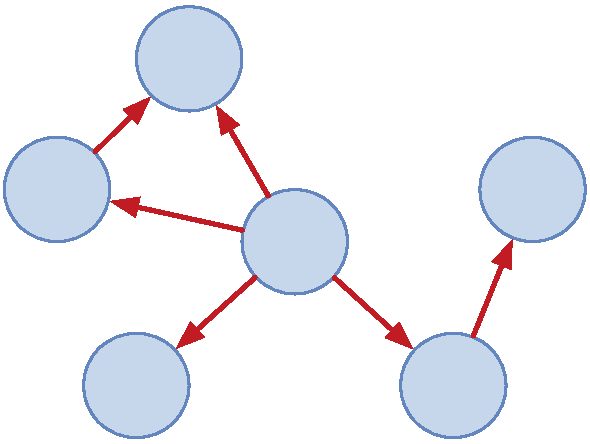
\includegraphics[width=0.5\textwidth]{cover-1.pdf}
    \caption{GRNs~拓扑结构示例图, 其中节点代表生物化合物, 边代表它们之间的关系。
    }
    \label{cover-1}
\end{figure}
\begin{figure}[!htbp]
    \centering
    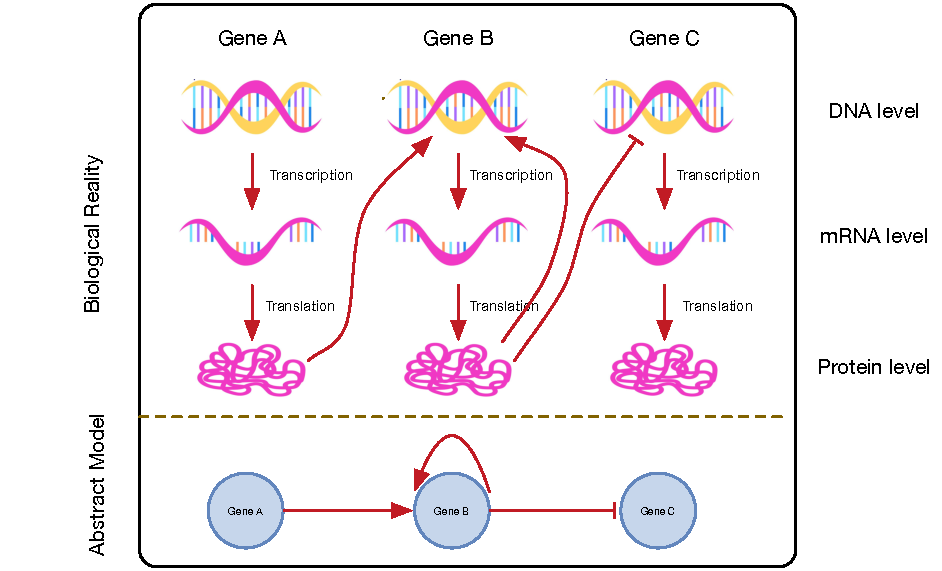
\includegraphics[width=0.95\textwidth]{cover-2.pdf}
    \caption{GRNs~构建的主要目标是为实际生物过程生成抽象模型。
    这些模型试图表示生物过程分子实体之间复杂的相互作用,比如基因激活、抑制或反馈环路。
    }
    \label{cover-2}
\end{figure}

从数据上,微阵列芯片~(microarray)~技术和单细胞~RNA测序~(scRNA-seq)~技术的发展产生的大量基因表达数据,
这些基因表达数据不仅可用于分析基因表达的时空规律,研究基因的功能,而且还可用于基因之间的相互制约关系,
研究基因调控网络模型,为理解生物潜在的调控机制带来了机遇。
另外, 转录组学、蛋白质组学、相互作用组学、代谢组学等高通量的实验室技术可以为模型提供更多的先验信息,
有助于构建更加复杂、更准确地反应生命现象的基因调控动态网络。

% 基因调控网络建模(构建)是当前生物信息学研究的重要领域和关键问题。
% 构建基因调控网络,需要利用基因表达数据来学习和挖掘基因间的调控关系,并借助于可视化技术展现基因调控网络的拓扑结构,进一步可促进基因功能的新发现和疾病相关的潜在基因的预测 \cite{lee2009computational}。

基因调控网络的构建,立足于阐明基因表达调控的作用关系,
有利于从网络的角度去了解复杂而精密的生物网络系统所蕴涵的结构和功能信息,
彻底了解网络的生物学意义,节省大量的实验费用与资源,
也可以利用模拟结果有效地指导进一步的生物实验,更好地了解生物系统的功能,
尤其是在肿瘤等复杂疾病研究中~\cite{boyle2017expanded},
例如癌症细胞的分化、扩散和增生等~\cite{hurley2011gene}。
通过基因调控网络建模,分析细胞代谢通路,在分子水平上理解癌症发生的机理,揭示癌症的内部机制,将进一步增强对癌症的整体认识,
发现诊断、控制和治疗癌症的方法~\cite{kreeger2009cancer,yan2016biological}。
此外,基因调控网络建模还有助于肿瘤药物的筛选和研制,能为攻克癌症等复杂疾病做出贡献。

总之, 基因调控网络建模是一门理论研究与实践应用相结合的学科,它不仅有重要的学术意义,
还有很高的商业价值,以及广阔的发展前景。
随着后基因组时代的到来,基因调控网络不仅可以为生物信息学提供大量的研究线索,
也可为特定生物问题提供强有力的理论依据,还可在疾病诊断、药物筛选等领域发挥更加广泛的作用~\cite{kreeger2009cancer}。

\subsection{国内外研究现状和发展动态}

基因调控网络建模是一种依靠数据挖掘进行的逆向工程研究, 即根据基因表达数据推理基因调控网络中的各类拓扑结构。
它首先通过生物实验获取高通量生物数据, 然后根据生物网络的先验知识, 针对特定生物问题建立数学模型, 
并设计合理的算法构建基因调控网络, 最后通过生物学实验验证逐步逼近和发现真实的基因调控网络~\cite{sima2009inference}。
从计算角度讲,基因调控网络推断依赖于已知的知识数据库发现~(Knowledge Database Discovery,~KDD)~工作流程。
KDD~从输入数据预处理到模型的验证, 通过数据库搜索比较之前的实验数据结果来完成的, 如图~\ref{cover-3}~所示。
\begin{figure}[!htbp]
    \centering
    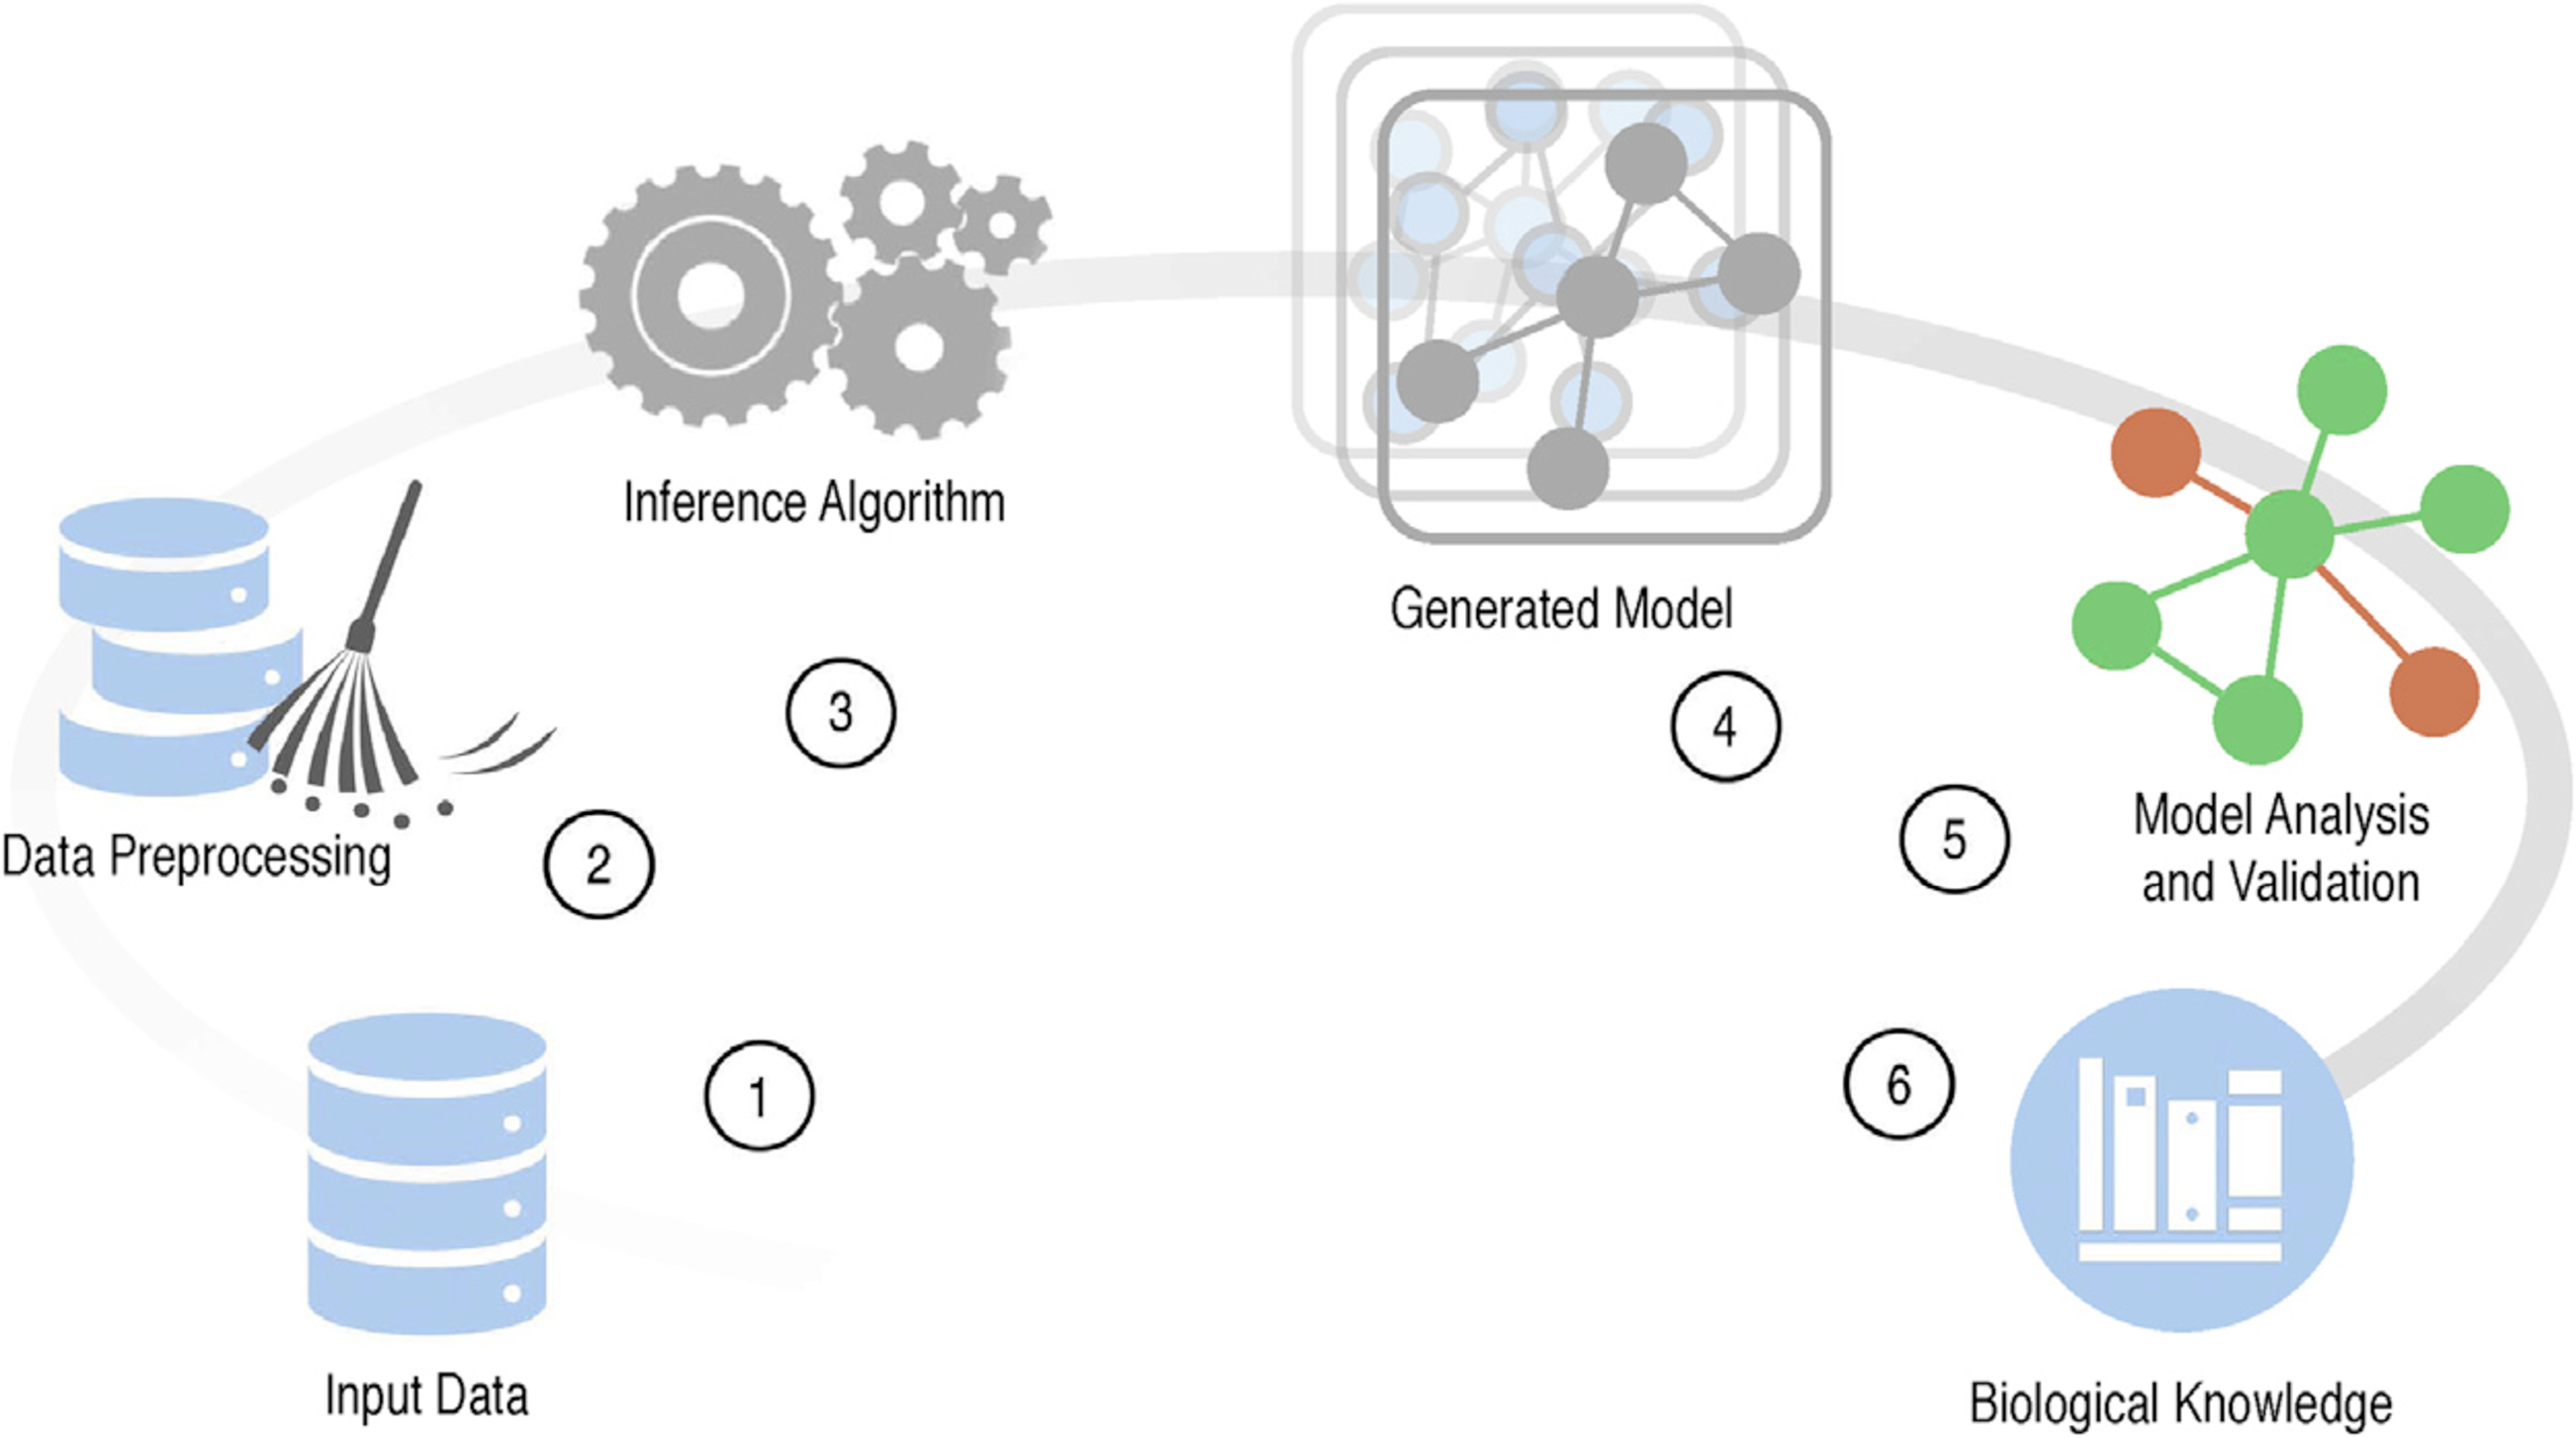
\includegraphics[width=0.95\textwidth]{cover-3.pdf}
    \caption{基于~KDD~工作流程的~GRN~重建步骤。
    \textcircled{\raisebox{-0.9pt}{1}}输入数据。
    \textcircled{\raisebox{-0.9pt}{2}}数据预处理。
    \textcircled{\raisebox{-0.9pt}{3}}网络推断算法。
    \textcircled{\raisebox{-0.9pt}{4}}生成模型。
    \textcircled{\raisebox{-0.9pt}{5}}模型分析和校验。
    \textcircled{\raisebox{-0.9pt}{6}}生物知识。
    }
    \label{cover-3}
\end{figure}

当前的基因调控网络建模牵涉到三方面的研究问题~\cite{schlitt2007current}:
\begin{enumerate}
    \item 根据数据源建立什么样的网络模型;
    \item 如何设计与实现网络建模算法;
    \item 如何评价和甚至是应用构建的网络。
\end{enumerate}

第三个方面属于应用范畴的研究,不是本研究的重点, 因此我们仅从前面两个方面讨论基因调控网络建模的相关研究现状。


\subsubsection{网络模型}

网络模型的建立首先需要我们对现在测序技术产生的数据及其特征有充分的认识。
在过去十几年中,高通量技术提供了巨大的数据,诸如下一代测序技术~(Next Generation Sequencing,~NGS)~\cite{BUERMANS20141932}, 
产生了显著质量、稳健性和低噪声的~DNA~和~RNA~样本数据。
测序已经成为一种标准方法,被认为是研究生命体的基石~\cite{CEREB2015923}。
测序产生的基因表达数据使生物学家能够大规模观察基因的表达水平, 对推断基因调控网络起到了至关重要的作用。
基因表达数据来源包括~DNA~微阵列,~RNA-seq~\cite{morin2008profiling}和~SAGE~(基因表达系列分析)~\cite{velculescu1995serial}。
在基因调控网络构建中我们将主要使用~DNA~微阵列数据~(microarray data)~和单细胞~RNA-seq~数据~(scRNA-seq),
同时也会结合其它比如~PPI~(蛋白质相互作用网络)~数据,~TF~(转录因子)~结合位点数据等作为先验知识。

(1) DNA~微阵列测序数据

% 生物微阵列又被广泛地称为生物芯片,是上个世纪~90~年代以来最为重要的基因测序技术之一,
% 其技术的关键点是将巨大的~DNA~分析缩小到芯片上, 在利用光电技术对信号进行探测, 最后通过计算机加以分析。
% 借助基因芯片技术研究者
% 从而建立基因表达谱以描绘基因组中的基因表达水平。
% 各种微阵列技术中, 用的最多的是基因微阵列芯片。
% DNA~微阵列测序数据最为常见, 使用微阵列测序数据进行基因调控网络构建也历史悠久源远流长。

DNA~微阵列技术(DNA microarray)~是上个世纪~90~年代产生的最为重要的基因测序技术,
是分子生物学在实验领域的重大突破,为探索生命本质和奥秘提供了基础保障。
该技术是在固相支持物表面集成大量的分子探针,与标记好的样品杂交,
来测定细胞内~mRNA~内的表达量也就是基因表达谱~(Gene Expression Profiles),
在不同条件下不同发展阶段和不同组织中的转录水平。
该技术能在同一时间内高效快速地分析大量基因的表达水平。
基因表达谱中蕴含了非常珍贵的信息,可以分析哪些基因的表达发生了更改, 
基因之间的表达有无相关性,基因的变化会对细胞产生怎样的变化,进而能帮助人们深入地认识诸如基因表达调控、发育、
疾病与癌症病理、衰老等生物过程~\cite{chen2005selecting,shen2009new,camargo2008identification}。
基因表达谱数据天生就有小样本、高维度、高噪声、高变异四个分析难点。

(2) 单细胞~RNA-seq~数据

单细胞~RNA-seq~技术在~2009年首先由~Tang等~\cite{tang2009mrna}提出,
但是在~2014~年以后由于新的协议和相对低廉的测序成本使得它在产业界和学术界都颇受欢迎,风靡至今。
单细胞~RNA-seq~技术与~DNA~微阵列测序技术最为显著的不同是,
后者测量的基因表达值是多个细胞基因表达值的平均值,
而前者测量的是单个细胞中的基因表达值。
单细胞~RNA-seq~测序技术也给数据处理带来诸多挑战,
比如大量的细胞异质性~\cite{wagner2016revealing},高度稀疏性导致的表达为零~(dropout\footnote{单细胞领域的~dropout~跟深度学习里面的~dropout~不是一个含义})~\cite{vallejos2017normalizing}, 细胞与细胞之间的测序深度变化, 细胞周期相关的批量效应~(batch effects)~\cite{buettner2015computational}。
在数据预处理阶段, 需要实现的目标不同和数据产生的场景, 对基因的~dropout值进行过滤或者填充~(dropout imputation), 或者需要对数据进行批量校正~(batch effects correction), 以提高后续下游分析的稳定性。
单细胞~RNA-seq~技术可以用来研究在转录组细胞特异性的变化中重要和新的生物学问题,
如鉴定细胞类型, 研究基因表达的随机性, 细胞发育轨迹推断~(trajectory inference),与细胞类型或者周期相关的基因调控网络的推断。
相比于微阵列测序数据而言,大多数情况下单细胞~RNA-seq~数据的计算分析需要开发新的方法。

寻找一个合适的网络模型是构建网络的首要问题。
在基因调控网络的研究中,为刻画和反应复杂生物网络的动态或静态行为,数学模型提供了一个强有力的工具。
不同的数学模型对基因调控网络进行了不同的表达和抽象,然而针对复杂的基因调控网络,
为对其进行全面描述,需要借助多个层次多种类型的模型来反应基因调控网络的不同特性。

从时空特性上区分,基因调控网络模型可分为:
静态模型与动态模型,例如,动态贝叶斯网是动态模型;
从图论角度区分,分为有向图模型和无向图模型;
从网络拓扑特性的角度出发,可构造出复杂网络和差异网络的模型。 
从建模所用的数据区分,模型可分为:
离散模型与连续模型,时序模型与非时序模型。
上面介绍的在基因调控网络构建中使用的两大类数据,~DNA~微阵列测序数据和单细胞~RNA-seq~数据, 
可以划分为时间序列数据~(time series data)~和非时序的扰动实验数据~(perturbation experiments data)~两种。
时间序列表达数据使生物学家能够调查生物网络中的时间模式,适合用来构建时序模型, 比如可采用微分方程模型建模; 
扰动表达数据提供了关于基因间调控方向的信息。
在单细胞数据中,序列的时间也可以是伪时间的, 比如在细胞发育轨迹推断中经常需要依赖伪时间推断算法, 来对细胞的时间先后及间隔进行标注。
非时序的扰动实验分为两类:基因操作~(即基因缺失,过度表达,温度敏感或动力学突变)~\cite{holstege1998dissecting}~或外部处理~(即环境胁迫)~\cite{gasch2000genomic}。

随着数据来源的多样化,模型改进和模型组合是当前网络模型的主要研究方向。
模型改进是针对现有的模型引入新的法则来构造新的模型,
而模型组合则是结合几个不同类型的模型取长补短达到性能最优。

\subsubsection{网络建模算法}
研究者们提出的基因调控网络的各类模型都在不同层次、不同程度上对真实的调控网络进行了抽象,
下文将针对关联网络、布尔网络、微分方程、贝叶斯网络、动态贝叶斯网络、回归方法的主要思想,
各类型方法的优缺点以及对应的研究现状做简要介绍。

(1) 布尔网络

布尔网络与微分方程相比则更为抽象,它对基因的状态做了进一步的简化,
用布尔函数代替了微分和导数来描述基因间的相互作用关系~\cite{shmulevich2002probabilistic,kim2007boolean,bornholdt2008boolean,zhou2016relative}~。
其中,基因的状态定量为两种不同的状态(``开"和``关")。
状态``开"表示一个基因转录表达, 状态``关"则代表一个基因未转录。
如果布尔网络模型进一步推广, 其可转变为时序布尔网络模型~TBN~(temporal Boolean networks), 这有利于处理多于一个单位时间跨度的基因间的依赖性。
图~\ref{fig:pre-bn}~展示了使用布尔模型方法的整体的工作流程。
\begin{figure}[!htbp]
    \centering
    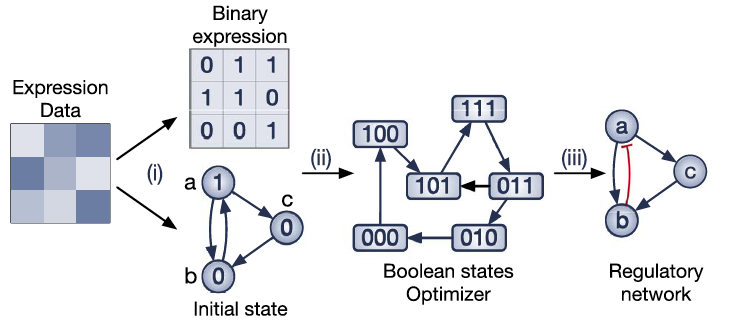
\includegraphics[width=0.9\textwidth]{pre-bn.png}
    \caption{
        使用布尔模型的方法的整体工作流程。
        (i)~这些方法首先对基因表达数据进行二值化,然后生成初始布尔状态。
        (ii)~这些方法针对二值对模型的状态进行优化。
        (iii)~这些方法输出带有激活和抑制边缘的GRN或一组布尔函数。
    }
    \label{fig:pre-bn}
\end{figure}

基于布尔网络模型的主要工作包括:
~Kauffman~\cite{kauffman2003random}~提出布尔网络的分析框架;
Akusu~等~\cite{akutsu1999identification}~证明了布尔网络推理所需要的最少样本数量;
Liang~等~\cite{liang1998reveal}~开发了~REVEAL~算法。
Shmulevich~等~\cite{marshall2007inference}~将马尔可夫链~(Markov Chains)~和布尔网络结合起来,引进了概率布尔网络模型~PBN~(probabilistic boolean networks),
比标准布尔网络模型有了更多的优越性。
在单细胞~RNA-seq~测序数据上,
Chen~等~\cite{chen2014single}~开发了~SingleCellNet,
采用遗传算法从预期的轨迹通过细胞状态构造概率布尔模型, 他们采用的布尔规则直接来源于文献。
Moignard~等~\cite{moignard2015decoding}~提出了~SCNS~算法,通过状态转换图分析轨迹来推断一个异步布尔模型。
连接状态转换图在这个算法中起着至关重要的作用,但是它很难从单细胞表达数据中获取。

布尔网络模型是最简单的网络模型,它通过布尔变量和布尔逻辑实现。
布尔网络建模时, 把基因的表达水平离散化成单一的表达和不表达两个数值,
而在现实的生物系统中,基因的表达过程是连续的,
对基因数据进行离散化时不可避免的会丢失很多重要的表达信息,
布尔网络模型不能完全捕获复杂的系统行为~\cite{lee2009computational};
网络中一个节点更新,会使得所有节点同步更新,而在实际的基因表达过程中,更新是异步进行的。

(2) 微分方程模型

微分方程模型是一种连续的确定模型, 具有强大灵活的优点,
通过抽象基因间的时序调控变化,相比布尔网络来讲, 适合描述更加精细的调控关系,可以较好地建模基因表达数据~\cite{gardner2003inferring,di2005chemogenomic,bansal2006inference, honkela2010model,lu2011high,li2011large}。
另外,通过加入新的变量,微分方程模型可以进一步描述环境变化对于基因表达水平的影响。

Chen~\cite{chen1999modeling}~最早使用微分方程系统作为基因表达调控网络模型。
若采用变量~$e_i$~表示第~$i$~个基因在~$t$~时刻的表达水平, 则~$n$~个基因之间的调控关系可以用微分方程描述如下:
\begin{equation}
\frac{{d_{e_i}}}{{dt}} = f_i (e),1 \le i \le n
\end{equation}

式中~$\frac{{d_{e_i }}}{{dt}}$~代表基因调控网络建模中,
第~$i$~个基因在~$t$~时刻表达水平的变化率,向量~$e=[e_1,e_2,...,e_n]^T$~则描述基因表达水平。
式中~$f_i(e)$~的表现形式表明了基因之间的调控机制和作用方式,也就是调控网络的结构。
调控函数~$f_i(e)$~最简单的形式是线性函数,可以表示为:
\begin{equation}
\frac{{d_{e_i }}}{{dt}} = \sum\nolimits_j {w_{ij} e_j} { + b_i } ,1 \le i \le n
\end{equation}

调控网络系统中各个基因之间的调控关系可采用参数~$w_{ij}$~表示,
激活、抑制和无调控关系分别对其取值为正、负或为零, $b_i$~表示基因的基础活性。
基因之间复杂的非线性作用关系可利用非线性的调控函数~$f_i(e)$~进行刻画和说明。
比如~Sigmoid~函数~(S型函数),来引入必要的非线性,具体表达形式为:

\begin{equation}
\frac{{d_{e_i } }}{{dt}} = AS(\sum\nolimits_j {w_{ij} e_j } + b_i) - D_i e_i ,1 \le i \le n
\end{equation}

图~\ref{fig:pre-df}~展示了使用微分方程模型方法的整体的工作流程。
\begin{figure}[!htbp]
    \centering
    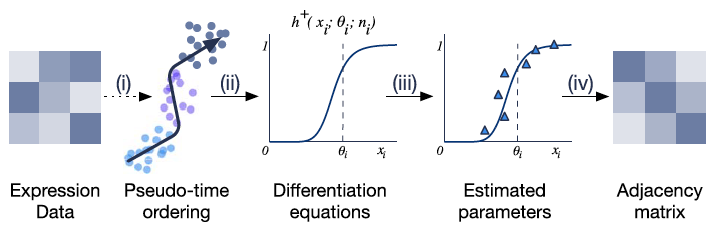
\includegraphics[width=0.9\textwidth]{pre-df.png}
    \caption{
        利用微分方程的方法的整体工作流程。
        (i)~针对单细胞数据集利用外部算法或软件推断细胞间的伪时序, 或者直接采用数据集提供的时间标签特征。
        ~DNA~微阵列测序数据直接采用提供的时间标签特征。
        (ii)~方法利用微分方程描述基因之间跟时间的关系。
        (iii)~使用不同的优化技术进行参数估计。
        (iv)~根据使用优化后的参数结合微分方程推断出基因之间的关系, 输出关联矩阵。
    }
    \label{fig:pre-df}
\end{figure}

在单细胞测序数据集上, 
为了从时间序列数据构建网络,~SCODE~\cite{matsumoto2017scode}~和~SCOUP~\cite{matsumoto2016scoup}~
分别引入~ODEs~和~SDEs~来计算基因之间的相关性。
SCODE~将某一基因在某一时间点的基因表达水平建模为对其他基因表达水平的线性依赖关系,
然后使用线性回归来估计基因之间的相关性矩阵;
SCOUP~则将各基因表达水平随时间的分化建模为一个连续的随机扩散~Ornstein-Uhlenbeck~(OU)~过程,
其中的某一个基因在某一时间点的表达量可以通过当前~OU~过程的正态分布来估计,
然后利用计算出的所有细胞的~z~值得到基因之间的相关性。

微分方程其主要的优点在于强大灵活,有利于描述基因网络中的复杂关系,能够很好的表现出基因之间的连续动态关系;
其缺点是难以适应中大型网络的构建, 计算量较大, 捕捉基因表达数据中包含的随机信息欠佳。

(3) 贝叶斯网络

贝叶斯网络~(Bayesian Networks, BNs)~是一种重要的概率模型~\cite{kim2003inferring,zou2004new,chen2006effective,needham2007primer,lo2015high},
由条件概率分布和网络结构两部分组成。
自从~Friedman~等~\cite{friedman2000using}~将贝叶斯网络应用到基因调控网络的重构中后,
贝叶斯网络在生物学上的应用越来越广泛,成为现今构建细胞调控网络最有效的方法之一。
在贝叶斯网络模型中变量之间的结构用有向无环图~(directed acyclic graph,DAG)~来表示,
变量之间的关系使用联合概率分布来描述。
相对于布尔网络的粗放定性,微分方程的精细定量,贝叶斯网络模型可看做这两者的折衷。

Cooper~等提出的~K2~算法~\cite{cooper1992bayesian}~是一个基于搜索评分的经典算法,
该算法为评价模型与数据的符合程度,
首先在给定先验信息和节点顺序的情况下,通过后验概率作为评分标准并利用贪婪搜索方法找出最佳网络结构。
%Peer~\cite{pe2001inferring}等人将贝叶斯网络技术用来处理调控网络中的扰动。
% 他们首先将数据离散化后根据评分函数挑选出最佳的的基因网络。
Imoto~等~\cite{kim2003inferring}~用非参数回归模型来解决离散化造成的阀值选取与信息丢失问题,
Imoto~等采用这一模型能获得基因之间的线性与非线性结构特征。
Jansen~等~\cite{jansen2003bayesian}~为利用贝叶斯网模型构建调控网络,
分析和计算各类基因表达数据以及蛋白质相互作用数据,并通过生物实验验证了模型的预测结果。
2004年~Friedman~等~\cite{friedman2004inferring}~为构建静态基因调控网络,
首次基于微阵列数据将贝叶斯网络模型用来预测基因调控关系。
Hartemink~等~\cite{hartemink2005reverse}~采用~BDe评分测度作为学习的目标函数,
通过对基因表达数据进行离散化及模拟退火算法来构建基因调控网络。
Werhli~和~Husmeier~\cite{werhli2007reconstructing}~将基因表达数据与来自多种数据源的先验生物学知识结合起来使用贝叶斯网络模型利用马尔科夫链蒙特卡洛~(MCMC)~抽样方案来抽样来自后验分布的超参数,
这种与多数据源的结合降低了基因调控网络参数学习的误差率,提高基因调控网络重建的准确性。
Yavari~等人~\cite{yavari2008gene}~根据基因本体将基因进行聚类,
并使用贝叶斯网络推断共聚簇基因之间的相互作用。
这种方法可以解决由于基因数目增加而导致的结构数量指数增加的问题。 
此外,他们还提出了一种在推理过程中使用共聚基因之间的互相关性的新方法。
共聚簇基因之间的互相关性为贝叶斯网络提供了时间延迟信息。 
由此模型产生的精度和灵敏度均有提高,而且结果表明这种模型适合对大规模基因进行建模。
杨等人~\cite{yang2011bayesian}~建议使用稀疏图搜索~(SGS)~算法减少贝叶斯网络的计算时间。
SGS算法利用迭代统计独立性测试和搜索技术来寻找最佳的网络结构。
最佳的基因调控网络是使用搜索-打分和基于约束两种方法混合产生的。
基于搜索和打分是使用优化技术在所有候选网络上搜索最佳网络结构并打分用来评估网络质。
基于约束的方法通过应用条件独立性检测来取代传统的统计或信息论度量来检测边的存在。
结果表明,他们提出的方法提高了准确性和计算效率。
Tan~和~Mohamad~\cite{kunga2012using}~使用贝叶斯网络结合爬山法和~Efron~的~bootstrap~抽样方法来构建基因调控网络。
他们首先使用最小局部平方~(LLS)~插值算法来处理微阵列数据集中存在的缺失值, 
然后采用贝叶斯网络建立网络模型并采用爬山算法进行学习, 
bootstrap~抽样方法被用来抽取高置信度的边集合。
他们的基因调控网络构建方法获得了较高的真阳性率, 并且揭示了基因之间更新的关系。 
Young~等~\cite{young2014fast}~提出一种基于贝叶斯网络的~ScanBMA~算法,
该方法采取数据变换和新的策略在模型空间搜索时高效快速,
可应用于大规模的基因调控网络推断。

贝叶斯网络模型的优点是灵活性好, 具有从数据中推导模型的能力, 能够自然地融入先验知识并能用专家知识和数据挖掘来改进模型的性能;
可以通过借助问题领域自身结构特征和变量间直接影响的局部性, 同时使用条件独立的数学概念, 将聚合概率分布的计算问题,分解为若干局部条件概率分布的计算问题;
模型结构和参数具有明确的含义可解释性好, 具有良好的学习能力; 能很好地处理隐变量和数据缺失问题。
研究发现与关联网络相比, 贝叶斯网络在识别准确度上常有更优异的表现, 尤其是在网络规模较小时。
其不足之处是:~许多贝叶斯网和动态贝叶斯网常采用离散模型, 对基因表达数据离散化导致损失了部分信息,
同时也降低了网络建模的准确度;
没有时序的概念,特别是对于存在伪时序的单细胞数据集而言,不能明显地表现基因调控网络的动力学特征。

(4) 动态贝叶斯网络

动态贝叶斯网络~(Dynamic Bayesian Network,~DBN)~模型是在静态~BN~网络模型中引入时间因素而形成的动态网络~\cite{dondelinger2010heterogeneous,grzegorczyk2010improvements}。
DBN~可以很好的表示随机系统的动态特性,也使用图模型的方式来表示模型中随机变量之间的概率依赖关系~\cite{hecker2009gene}。
DBN~更好地刻画了基因调控网络的动态特性,善于处理非线性关系和由随机现象引起的不确定性,能够描述基因之间的负反馈调控过程,
相比于静态贝叶斯网它能够克服其有向无环的缺点,具有很好的概率推理能力和知识表达能力,使得模型的预测精度进一步提高。

Friedman~和~Murphy~等~\cite{friedman2004inferring}~考虑到了基因调控存在一定的时延性,
从理论的角度分析了~DBN~从时序基因表达数据构建基因调控网络的问题, 提出用动态贝叶斯网络模型分析时序基因表达数据。
Smith~等~\cite{smith2006computational}~用动态贝叶斯网络模型来分析微阵列数据,
结合了基因调控的负反馈与时延因素, 因此需要采用网络中不同节点来表示同一基因不同时间点的表达向量。
Wu和Liu等~\cite{wu2008dynamic}~改进了动态贝叶斯网络建模方法,使用了~MCMC~和带重启的贪心爬山算法两种不同的模型搜索方法。 
两种方法在时间效率上不相上下,与带重启的贪心爬山算法相比~MCMC~具有更高的预测精度。
Song~\cite{song2009keller}结合微阵列数据与基因关系的先验知识在~DBN~上提出新的数据整合模型,利用并行算法,构建基因调控网络。
Kim~等~\cite{del2010efficient}~也在这方面做了大量的工作,
并结合线性或非线性模型以及相应的生物学知识对动态贝叶斯网络进行了改进。
Norbert~\cite{netrapalli2010greedy}~为从基因扰动型实验数据中学习动态贝叶斯网络,
利用~Husmeier~\cite{werhli2006comparative}~提出的离散化方法来对基因表达数据进行预处理,
并使用~BDe~测度来进行评分搜索,最终构建动态贝叶斯网络, 这种搜索方法实现了减少学习时间,降低计算的时间复杂度的目的~\cite{hurley2011gene}。
Grzegorczyk~和~Husmeier~\cite{grzegorczyk2010improvements}~通过将多变点过程与可逆跳跃马尔可夫链蒙特卡罗方法~(RJMCMC)~结合,改进了基于动态贝叶斯网络推断的方法。 他们通过引入动态编程方案来优化RJMCMC上的收敛性,该方法从正确的条件分布对变化点进行采样。 
此外,引入了贝叶斯聚类的新方法以促进节点之间的信息共享, 使得模型复杂度能够自动调整。
Chai~等~\cite{chai2012inferring}~提出了缺失值插补的动态贝叶斯网络模型,
利用缺失值插补来提高基因调控网络推断中的计算效率,
同时通过限制潜在调控因子的表达变化来缩短计算时间。
Vinh~等~\cite{vinh2012gene}~将动态贝叶斯网络方法与基于时间序列表达数据的基因调控网络构建的全局最优化相结合,
他们在全局优化框架上使用互信息测试来学习高阶带延时的基因相互作用。
他们的方法能够改善动态贝叶斯网络只适合于小规模网络的缺陷,
同时能够避免动态贝叶斯网络结构学习容易陷入局部最优的状况。

(5) 关联网络

关联网络~(relevance network)~主要借助基因表达数据间相关性的计算来构建模型。
相关性分析是构建基因调控网络最常见的方法之一。
计算基因间的相关性常通过互信息、皮尔逊相关系数等测度来进行。
主要思路是:~对于预先设定的阈值,若基因间相关性不在阈值范围内,则在网络中基因间有边相连。
若两基因间具有相同或相近的调控机制,则两个基因相关性较高,
尤其是,对于同一转录因子的靶基因或同一条生物通路上的基因,它们的相似度或相关性较高。

皮尔逊相关系数~(PCC)~是一种线性相关系数, 它反应了两个变量间的线性相关程度。
设~$X$,$Y$~为随机变量,~$pcc(X,Y)$~定义如下:

\begin{equation}
pcc(X,Y) = \frac{{\sum\limits_i {(x_i -\bar x_i )(y_i -\bar y_i )} }}{{\sqrt {\sum\limits_i {(x_i  - \bar x_i )^2 } } \sqrt {\sum\limits_i {(y_i  - \bar y_i )^2 } } }}
\end{equation}

其中,~$\bar x_i$、$\bar y_i$~分别是~X、Y~的均值。
~$pcc(X,Y)$~的取值在~-1到~1之间。
当~$pcc(X,Y)$~为~-1~或者~1~时, 表示两个变量完全相关;
当~$pcc(X,Y)$~为~0~时, 表示两个变量完全无关。

PCC~被广泛用于评估变量之间的线性关系~\cite{stuart2003gene},但在不借助其他信息的情况下无法区分直接关系和间接关系,而偏相关分析法~(PC)~\cite{baba2004partial}~通过考虑附加信息条件来有效区分直接和间接关系。
另外, Barabási~等~\cite{barzel2013network}~提出了一个基于动态关联性的方法,该方法通过消除网络中的间接影响进行直接关联性和间接关联性区分; 
Feizi等~\cite{feizi2013network}~提出了利用网络卷积去除所有关联之间的综合效应区分直接和间接关联性。
这两种方法~\cite{barzel2013network,feizi2013network}~只能测量线性直接关联性,
但无法测量非线性关联性, 而非线性关联性在许多非线性系统比如生物系统中发挥着重要的作用。
基于~PCC~和~PC, 距离相关性~\cite{szekely2007measuring,kosorok2009brownian}~和部分距离相关性~(Pdcor)~\cite{szekely2014partial}~被提出用于度量随机向量间的相关性,这些统计量对于依赖偏离很敏感。
Pdcor~的评估存在假阳性,即当向量~$X$~非条件独立时, Pdcor(X;Y|Z)~也有可能为零~\cite{szekely2014partial}。

互信息~(Mutual Information,~MI)~常用来刻画和描述两个系统间的统计相关性,或通
过熵来反应一个系统中蕴含的另一个系统信息量的大小, 设~$P(x)$~是~$X=x$~的概率,
则随机变量~$X$~的熵定义为~\cite{cover2012elements}:
\begin{equation}
H(X) = - \sum\limits_x {P(x)\log _2 P(x)} 
\end{equation}

设~$P(x,y)$~是~$X=x$,~$Y=y$~时的联合概率,则~$X$,~$Y$~的联合熵定义为:
\begin{equation}
H(X,Y) =  - \sum\limits_x {\sum\limits_y {P(x,y)\log _2 P(x,y)} } 
\end{equation}

随机变量~$X$~和~$Y$~的互信息为:
\begin{equation}
MI(X,Y) = H(X) + H(Y) - H(X,Y) = \sum\limits_{i,j} {P(x_i ,y_i )\log \frac{{p(x_i,y_i )}}{{p(x_i )p(y_i )}}} 
\end{equation}

需要注意的是在基因调控网络推断中由于基因表达数据是连续的,而互信息在计算时需要离散化,
一般使用~B-样条平滑和离散化方法来进行计算~\cite{daub2004estimating}。
由于互信息能够捕获有效捕获变量间的非线性相关性,
因此在复杂的基因调控网络相互作用推断中其应用十分广泛~\cite{brunel2010miss,zhang2011inferring}。

图~\ref{fig:pre-gc}~展示了关联网络模型方法的整体的工作流程。
\begin{figure}[!htbp]
    \centering
    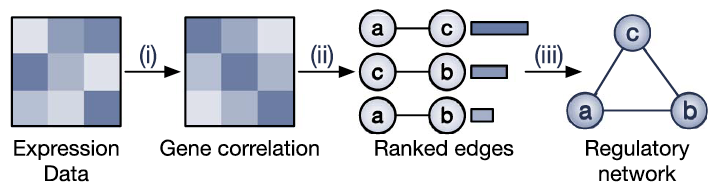
\includegraphics[width=0.9\textwidth]{pre-gc.png}
    \caption{
        利用基因表达相关的方法的整体工作流程。
        (i)~首先通过计算每个基因对的表达相关性来初始化边缘的权重。
        (ii)~进行假设检验,估计每个边缘的显著性,然后使用预定义的显著性阈值去除被认为不显著的边缘。
        (iii)~方法输出最大的连接分量。
    }
    \label{fig:pre-gc}
\end{figure}


Butte~等~\cite{basso2005reverse}~首先利用互信息计算所有基因对之间的相关性,然后设置互信息阈值。
为构建关联基因调控网络, 通常定义高于阈值的基因对之间存在关联并使用边连接起来构成网络。
Margolin~等~\cite{margolin2006aracne}~提出的~ARCANE~采用~Data Processing Inequality~(DPI)~来过滤间接作用边。
Faith~等~\cite{faith2007large}~提出的~CLR~方法使用互信息的经验分布来过滤间接作用边。
Meyer~等~\cite{meyer2007information}~提出的~MRNET~方法使用最小化冗余特征选择算法~\cite{peng2005feature},
在计算后的互信息网络上对每一个目标基因选择一个同目标基因关联最强但与已经候选的基因集合冗余性最低的基因,这个过程不断进行迭代。
Altay~等~\cite{altay2010inferring}~提出的~C3NET~和其扩展算法~BC3NET~\cite{de2012bagging}~结合一个最大化的步骤来估计互信息从而使预测更准确。

MI~被广泛用于评估变量之间的非线性相关性,
它是基于统计独立性进行计算。
需要注意的是,在只有联合概率时无法计算直接变量之间的~MI,
并且~MI~和~PCC~一样有假阳性~\cite{frenzel2007partial,schreiber2000measuring}。
~Zhao~等提出了条件互信息~(Conditional Mutual Information,~CMI)~\cite{zhang2011inferring}~和部分互信息~(Part Mutual Information,~PMI)~\cite{zhao2016part},
这两个测度在互信息上引入了条件计算的机制减少了假阳性边,
能有效检测变量之间非线性的间接或直接的相互作用。
他们将这两个测度与基于贪心策略的路径一致性算法~(Path Consistency Algorithm,~PCA)~结合起来先后提出了~PCA-CMI\cite{zhang2011inferring}~和~PCA-PMI\cite{zhao2016part}。

在单细胞测序数据集上,
Yu~等提出了~NLNET~方法\cite{yu2013hierarchical}, 
两个基因之间的相关性被定义为基于条件有序列表~(Conditional ordered list,~DCOL)~的距离,
其中基因~G1~到基因~G2~的距离取决于通过~G1~中所有样本的表达顺序。
NLNET~使用的这种距离度量没有考虑到的点是,真实生物网络中的一个基因可能与多个基因相互作用。
Thalia~等~\cite{chan2017gene}~提出了高效的~PIDC~算法,
该算法利用偏信息分解~(partial information decomposition,~PID)~测度来衡量基因之间的关系。
Guo~等~\cite{guo2015sincera}~提出了~SINCERA~方法, 该方法利用低阶偏相关性~(low-order partial correlation),可以在测量中涉及两个以上的基因,是一种更符合实际的方式来呈现复杂网络的相互作用。
在~SINCERA~方法中,给定第三个基因~G3,基因~G1~和基因~G2~之间的相关性是~G1~与~G3~的线性回归
所产生的残差与~G2~与~G3~的线性回归所产生的残差之间的相关性。
SINCERA~假设基因之间存在线性依赖关系,并使用最小平方估计来计算目标基因和条件基因的回归系数。

可以看出,虽然关联网络建模操作简单易行,但不管是基于~PCC、MI~还是~PID~等测度构建的网络极其容易引进假阳性边。
虽然各种方法都站在不同的角度来尽量减少假阳性边来提高网络构建的准确性,
但是随着网络规模的扩大这种状况还是在不断恶化,网络构建的准确性急剧下降。

(6) 回归方法

近年来在~DREAM~系列竞赛的推动下,利用机器学习回归模型进行基因调控网络的构建方法大量地涌现出来。
这类方法本质上可以看作是关联网络模型的延伸,
但是与关联网络只关注量化相互作用不同的是,回归方法能够推断出基因之间的相互作用方向。
回归模型将基因调控建模转化为机器学习特征选择的问题,
即是将靶标基因的表达看作是调控基因表达之间的相互线性作用或者非线性作用的结果,
然后采用~bagging~或者~boosting~的做法,推断出最终的基因调控网络。
它们应用在基因调控网络构建上优点是计算效率高,网络构建准确率高;
缺点是一些非线性的模型可解释性较低参数意义不明确,并且缺少对生物结构的支持。
回归模型成功应用于基因调控网络构建中的典型算法包括基于随机森林的~GENIE3~\cite{Huynh-Thu2010},
基于~Lasso~回归的~TIGRESS~\cite{Haury2012}。
在处理时间序列数据上有~GENIE3~的扩展方法~GENIE3-lag~\cite{huynh2012machine},
与扩散模型相结合利用随机森林来学习隐含参数的~Jump3~\cite{Huynh-Thu2014}。

在单细胞~RNA-seq~测序数据集上, 
SCENIC~\cite{aibar2017scenic}~融合了~GENIE3,~RcisTarget~和~AUCell~三个算法来在单细胞测序数据上实现了基因调控网络的构建和基因的聚类。
单细胞~RNA-seq~也能产生基于时间序列的~RNA-seq~数据。
与传统的时间序列数据相比,基于单细胞的时序数据在单个时间片上产生了更多的样本,测序的总体成本也变得十分昂贵。
因此也有很多方法利用原始数据推断出伪时序~(pseudo-time ordering)~后,再利用回归方法构建基因调控网络。
LEAP~\cite{specht2017leap}~简单地使用皮尔逊相关性来计算每个时间窗口的基因之间的相关性。 
然后,它通过收集所有时间窗口内所有基因对的最大相关性来合并所有相关矩阵。
SINCERITIES~\cite{papili2017sincerities}~利用基因在不同时间片上的表达分布之间的距离来构建基因的表达矢量,
然后使用格兰杰因果关系~(Granger causality)~的思想结合线性回归模型来推断基因调控网络。
SINCERITIES~并没有直接来计算在每个时间窗口中基因间的相关性。
SCIMITAR~\cite{cordero2017tracing}~使用连续的多变量高斯混合模型对数据进行建模,
然后使用期望值最大化~(EM)~算法估计参数。
EM~算法估计了每个分布的参数,以及一个细胞属于每个分布的可能性。
SCIMITAR~从混合模型的协方差矩阵中计算出每个伪时间的相关矩阵,
然后该方法通过计算协方差矩阵之间的距离来计算相似度矩阵,
最后使用相似度矩阵的频谱聚类~(Spectral Clustering)~来确定整个时间轨迹的发展阶段。
对于每个发展阶段,该方法通过对该阶段的相关矩阵进行平均,最终输出共识网络。
SINGE~\cite{deshpande2019network}~使用回归模型来确定一个时间窗口内两个基因之间的相关性。
对于每个目标基因,该方法利用基于核函数的格兰杰因果关系~(Granger causality)~回归来计算该基因与所有其它基因的相关性。
然后采用~Borda~计数聚合方法~\cite{van2000variants}~来对调控边打分,
该方法偏重于多次格兰杰检验一致性排名靠前的边,对两个基因之间的连接进行随时间的排序。
上述四种方法中, SCIMITAR~自身能直接从输入的数据中推断出细胞的伪时序, 
而~LEAP、SINCERITIES~和~SINGE~都依赖用户在输入时提供细胞的时间排序。

\subsection{主要研究工作}
本课题的主要研究内容是基因调控网络构建。
从系统生物学的角度出发,通过计算方法研究基于~DNA~微阵列数据以及
单细胞~RNA-seq~测序数据上的基因调控网络的构建、评估及其在复杂细胞类型分析等生物问题中的应用。
我们以复杂网络理论、信息论和机器学习方法为基础,以数据的结构特性和数据本身的特点为研究对象,
构建合适的网络推断模型和调控网络构建方法,
并同已有的方法进行评估和对比。

(1) 基于互信息的网络推断算法研究

通过对基于信息理论互信息的网络推断算法进行研究后发现,
由于原始数据中存在的外部噪声、
网络结构中的拓扑稀疏性和非线性基因之间的依赖等因素,
现如今这类方法在网络推断中会引入冗余的依赖关系。
特别是随着网络规模的增加,这些方法的表现大幅降低。
我们提出了一种新的基于互信息的网络结构推断方法~Loc-PCA-CMI:
首先识别局部重叠基因簇~(local overlapped gene clusters),
然后基于条件互信息~(PCA-CMI)~的路径一致性算法推断每个簇的局部网络结构,
最终通过聚合局部网络结构,也就是基因之间的依赖性网络,来构造最终的~GRN。

(2) 基于数据驱动的网络推断算法研究

最近关于数据驱动的动态网络构建的研究为我们提供了解决回归问题的新视角。
当前基于数据驱动方法无法构建全局网络,
我们提出了一种数据驱动的基因调控网络构建方法~D3GRN。
该方法使用了抽样的策略~(bootstrapping),
将每个目标基因的调控关系转化为函数分解问题并利用揭示网络相互作用的算法解决各个子问题。
为了弥补数据驱动方法无法构建全局网络的缺陷,
我们最后采用了抽样策略和基于面积的评分方法来推断最终的网络。


(3) 基于相似性学习的单细胞聚类算法研究

单细胞数据聚类是单细胞数据上游分析的核心任务, 
在很大程度上是构建与细胞类型相关的基因调控网络的必要步骤。
相似性学习是当前单细胞聚类算法研究的重点。
针对当前单细胞~RNA-seq~数据集上细胞聚类不够准确鲁棒的问题,
我们使用多种相关性度量方法来刻画细胞的特征, 
然后使用随机森林回归模型进一步学习细胞与细胞之间的相似性矩阵,
基于相似性矩阵后采用层次聚类来决定细胞的最终类别。

(4) 基于异常检测的单细胞稀有细胞识别算法研究

现有的寻找稀有细胞的算法大部分依赖单细胞聚类方法,
在处理超大规模~scRNA-seq~数据时候非常耗时或耗费内存。
在这项研究中,我们提出了一种高效准确的基于孤立森林的方法~DoRC。
DoRC~产生的稀有度分数可以帮助生物学家们只关注超大规模~scRNA-seq~数据内一部分的细胞, 也就是稀有细胞,进行后续分析。
为了在随后的下游分析的过程中,我们可以使用细胞聚类方法~RafClust~进一步区分稀有细胞类型。

(5) 基于矩阵分解的单细胞基因调控网络方法研究

识别细胞类型特征和细胞的基因表达活动程序~(如生命周期过程、对环境因素的反应)~对于理解细胞和组织的组成至关重要。
虽然单细胞~RNA-seq~数据可以量化成单个细胞中的转录本,
每个细胞的表达谱可能是这两种类型的程序的混合物,使它们难以分离。
在这里, 我们提出了一个使用矩阵分解的算法~WSSMFA~来解决这个问题。
通过模拟表明, 我们提出的~scGRNHunter~方法可以准确地推断出身份和活动性的子程序, 
并在此基础上构建基因调控网络。

这五个方面的研究工作对应了五种方法,它们之间的在研究思路上的宏观关系如图~\ref{fig:pre-structure}~所示。
涉及到两大类的数据, 无向网络推断的有~Loc-PCA-CMI~方法, 有向网络推断有~D3GRN~和~scGRNHunter~两种方法, 
由于~scGRNHunter~涉及到与单细胞聚类相关的讨论, 我们首先提出了单细胞聚类方法~RafClust。
单细胞稀有细胞的识别方法~DoRC~中利用了~RafClust~来确定稀有细胞的细胞类型,
一定程度上可以认为~DoRC~是~RafClust~方法的一个具体的应用场景。
\begin{figure}[!htbp]
    \centering
    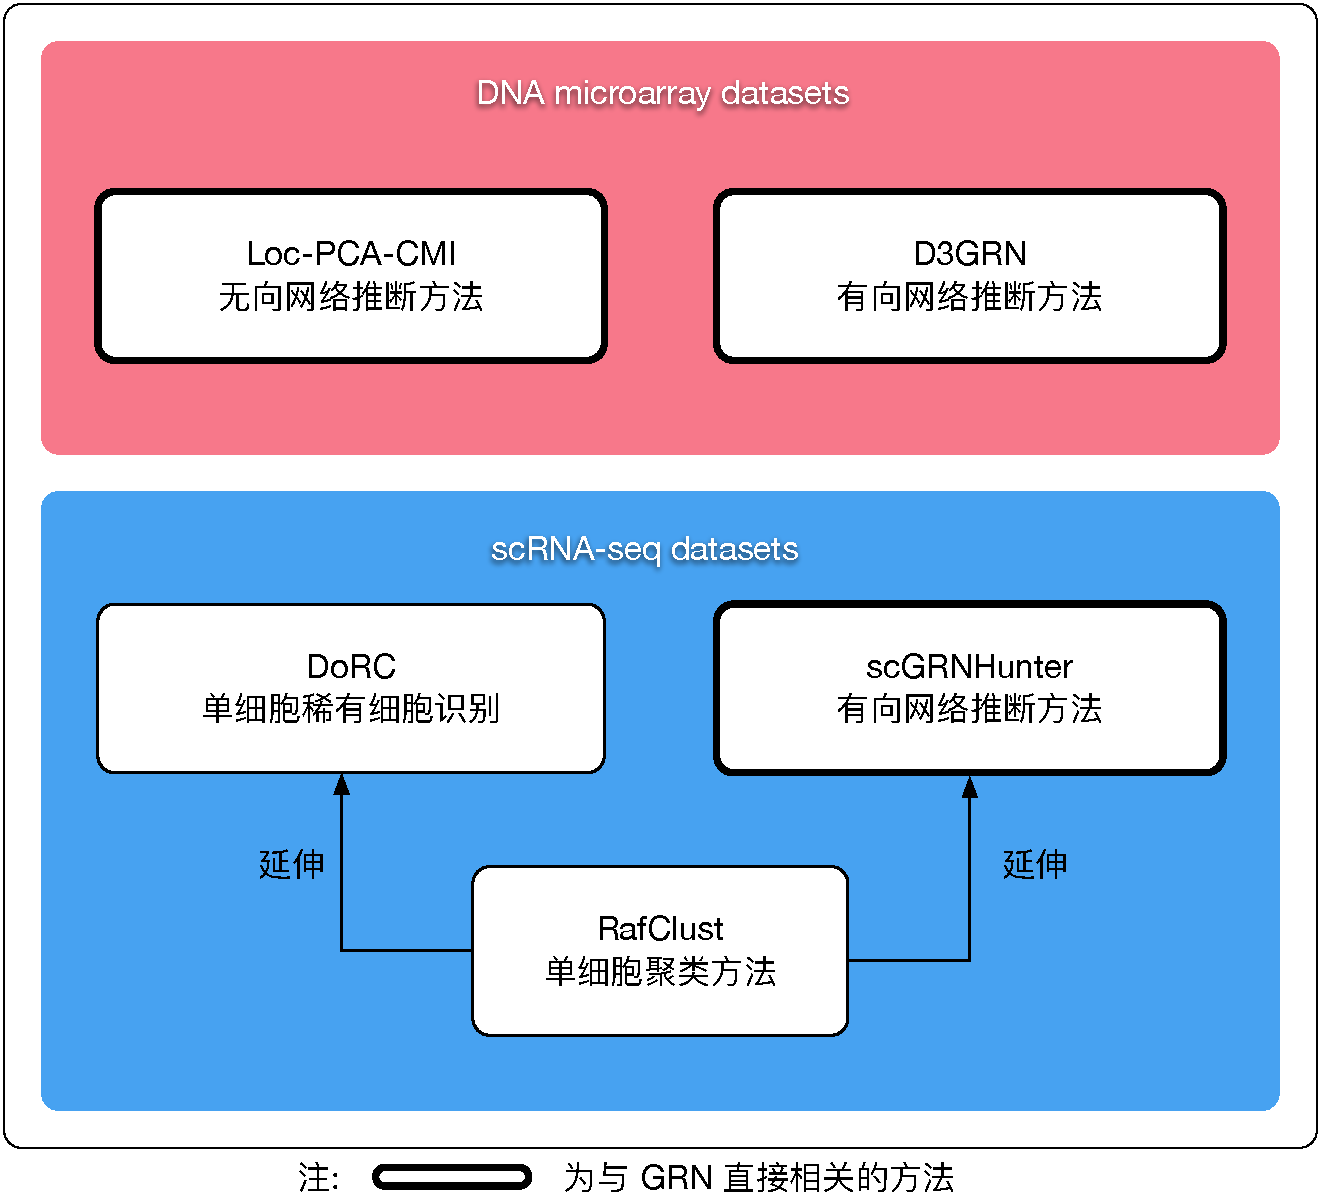
\includegraphics[width=0.8\textwidth]{pre-structure.pdf}
    \caption{主要研究工作宏观关联示意图。
    }
    \label{fig:pre-structure}
\end{figure}

\subsection{论文组织结构}

全文内容共七章,各章内容简述如下:

第一章~绪论。
主要描述了基因调控网络研究在目前的研究背景与意义, 国内外研究现状和发展动态。
最后,介绍本论文的研究工作,并给出全文的结构安排。

第二章~基于互信息和局部结构融合的基因调控网络结构推断方法。
主要介绍了基于互信息网络推断算法相关工作, 为了降低假阳性调控边的引入设计了
Loc-PCA-CMI~算法,介绍了算法细节,并对使用的数据集进行了介绍, 之后对实验结果进行了讨论和总结。

第三章~基于数据驱动的基因调控网络构建方法。
主要回顾了当前最热门的基于回归的基因调控网络构建方法的研究现状,
对比了~D3GRN~与其它几种方法的设计思路,并给出了~D3GRN~的算法细节,并对使用的数据集进行了介绍, 之后对实验结果进行了讨论和总结。

第四章~基于随机森林相似性学习的单细胞聚类方法。
主要回顾了当前单细胞~RNA-seq~数据集上的细胞聚类方法及其优缺点, 
RafClust~的设计思路以及~RafClust~方法详细的流程,并对使用的数据集进行了介绍, 并对实验结果进行了讨论和总结。

第五章~基于孤立森林的单细胞稀有细胞识别方法。
主要回顾了当前稀有细胞识别方向的方法及其优缺点, 
DoRC~的设计思路以及~DoRC~方法详细的流程, 并对使用的数据集进行了介绍, 并对实验结果进行了讨论和总结。

第六章~基于矩阵分解的单细胞基因调控网络构建方法。
主要提出了一种新的单细胞数据上进行身份~GEP~(gene expressin program)~和活动~
GEP~进行构建的思路, 并以此为基础详细介绍了~scGRNHunter~的几个步骤, 其中重点介绍了矩阵分解算法~WSSMFA。
最后我们介绍了数据集, 并对实验结果进行了讨论和总结。

第七章~总结与展望。总结全文并对未来的研究方向进行了展望。

\newpage
\section{一种新的基因调控网络结构推断方法}
\label{sec:locpcacmi}

从基因表达数据推中推断基因调控网络~(GRN)~的结构一直是系统生物学中的十分具有挑战的问题。
鉴定基因之间复杂的调控关系对于理解细胞的调控机制至关重要。
到如今,基于信息理论的各种~GRN~推断方法已经被提出来。
在上面一章里面, 我们回顾了各种网络模型和建模方法。
基于信息理论的~GRN~推断方法就是属于关联网络建模方法的范畴。
然而,在传统的DNA~微阵列测序数据中由于存在的外部噪声、
网络结构中的拓扑稀疏性和基因之间的传递依赖等因素,
这些方法在网络推断中会引入假阳性的依赖关系。
特别是随着网络规模的增加,这些推断方法的表现会大幅降低。
在本章节中我们提出了一种新的网络结构推断方法~Loc-PCA-CMI:
首先识别局部重叠基因簇,
然后基于条件互信息~(PCA-CMI)~的路径一致性算法推断每个簇的局部网络结构,
最终通过聚合局部网络结构,也就是基因之间的依赖性网络,来构造最终的~GRN。
我们在~DREAM3~敲除数据集上对~Loc-PCA-CMI~进行了评估,
将其性能与其它基于信息理论的网络结构推断方法,包括~ARACNE、MRNET、PCA-CMI~和~PCA-PMI,进行了比较。
实验结果证明,~Loc-PCA-CMI~在~DREAM3~数据集上特别是在基因数目为~50~和~100~的网络上表现优于其它四种基准方法。

\subsection{介绍}

推断和理解基因调控网络~(GRN)~是系统生物学中的一个关键问题, 
可以帮助生物医学科学家明确识别基因与基因之间复杂的调控关系、理解细胞中的调控机制~\cite{altay2010inferring, basso2005reverse}。
在过去,~GRN~是从实验干预中推断出来的,其中基因之间的调控相互作用被验证。
显然,这种方法是不可行的~\cite{elnitski2006locating},需要耗费大量时间和相当大的成本。
由于微阵列技术的发展,大量的基因表达数据通过测序被得到,这使得基于计算方法从这些表达数据中推断出~GRN~成为可能~\cite{maetschke2013supervised}。
% 近年来,基于计算方法的网络推断已成为最重要的目标之一~\cite{altay2010inferring, margolin2006reverse}。
% 已经提出了各种用于GRN推断的方法,例如基于回归的方法~\cite{Huynh-Thu2010, Haury2012, Huynh-Thu2014, liu2014group, li2017mgt, zheng2018bixgboost},
% 基于微分方程的方法~\cite{sakamoto2001inferring, chowdhury2015stochastic, li2011large},
% 贝叶斯和动态贝叶斯网络~\cite{murphy1999modelling, zou2004new, vinh2011globalmit, young2014fast, Liu2016, omranian2016gene},
% 以及基于状态空间的方法~\cite{wu2003modeling, quach2007estimating}。
% 不幸的是,
基因表达数据通常具有高维度和相对较小的样本量,存在``维度诅咒”的问题~\cite{wang2006inferring}。
此外,基因表达数据通常涉及大量外部噪声和非线性关系。
所有这些问题使得准确推断基因之间的调控相互作用,
尤其是在后基因组时代处理大规模基因表达数据时,
变得更加复杂和具有挑战性。


研究者基于各种不同的假设和不同的条件提出了从表达数据构建~GRN~精确结构的各种不同的计算方法~\cite{longabaugh2005computational,karlebach2008modelling}。
目前的这些方法可以大致分为基于模型~(model-based)~和无模型~(model-free)~两大类别。

基于模型的方法通常制定系统的计算模型并进一步学习这种模型的参数。
典型的计算模型包括布尔网络~\cite{shmulevich2002probabilistic,kim2007boolean,bornholdt2008boolean,zhou2016relative},
贝叶斯网络~\cite{kim2003inferring,zou2004new,chen2006effective,needham2007primer,lo2015high},
以及微分方程模型~\cite{gardner2003inferring,di2005chemogenomic,bansal2006inference, honkela2010model,lu2011high,li2011large}。
这些基于模型的方法的细节在上一章中有详细介绍,接下来我们重点介绍基于无模型~(model-free)~的方法。
% 布尔网络模型是最简单的网络模型,它通过布尔变量和布尔逻辑实现。
% 因为基因表达的状态被认为只是活动或非活动,布尔网络模型不能完全捕获复杂的系统行为~\cite{lee2009computational}。
% 贝叶斯网络模型是一种流行的概率图形模型,其中基因之间的依赖关系通过有向无环图描述。
% 贝叶斯网络模型在处理噪声和结合先验知识方面优于其它模型,
% 但该模型中的结构学习是计算密集型的,并且已被证明是~NP~难问题~\cite{chickering2004large}。
% 微分方程模型通过函数表征基因在特定时间的表达水平,其涉及与其它基因的调控相互作用。
% 通常,它将一个基因表达的变化率~(导数)~作为其它相关基因表达水平的函数。
% 使用微分方程模型重建~GRN~的一个主要挑战是如何在高维模型中有效识别模型结构和估计参数。
% 关于各种数据驱动建模方案和相关主题的文章评论,可以参考~\cite{hecker2009gene,marbach2012wisdom,wu2007inference,liu2012reverse,li2018control}。

基于无模型~(model-free)~的方法主要通过衡量基因之间的依赖性来识别调控相互作用,
典型的算法包括基于传统相关性和基于信息理论的方法。
在基于相关性的方法中,调控相互作用由两个基因之间的共表达程度决定,
例如~Pearson~相关性,秩相关性,欧几里德距离和一对表达值向量之间的角度~\cite{wang2014review}。
然而,基于相关性的方法无法识别基因之间的复杂依赖性,例如非线性依赖性~\cite{ruyssinck2014nimefi}。
此外,相当多的功能相关基因可能不会共表达,这使得难以准确推断调控相互作用。
基于信息理论的方法也是一种代表性的无模型~(model-free)~方法,其中互信息~(MI)~有利于衡量基因之间的潜在依赖性,
因为它可以有效地捕获非线性依赖关系~\cite{brunel2010miss,zhang2011inferring}。
近年来,已经提出了基于信息论的各种网络推断方法,
其侧重于区分直接调控相互作用与间接关联~\cite{marbach2010revealing}。
为消除间接相互作用,
Margolin~等人~\cite{margolin2006aracne}提出了~ARACNE~方法,使用数据处理不等式~(DPI)来过滤掉来自三重基因的间接相互作用。
Meyer~\cite{meyer2007information}~的最小冗余网络~(MRNET)~使用最小冗余特征选择方法~\cite{peng2005feature},
其中对于网络中的每个候选基因,它选择其高度相关基因的子集,同时最小化所选基因之间基于互信息的标准。
Zhang~等人~\cite{zhang2011inferring}~介绍了一种基于条件互信息~(PCA-CMI)~的路径一致性算法; 
Zhao~等人~\cite{zhao2016part}~引入了基于偏互信息~(PCA-PMI)~的路径一致性算法。
路径一致性算法~(PCA)~是一种穷举算法,广泛用于推断~GRN~\cite{zhang2011inferring}。
~PCA-CMI~和~PCA-PMI~这两个算法通常会在运行时间和准确度之间进行折中权衡。
随着网络规模的增加, 网络噪声本身在增加,
这类~top-down~的算法的复杂度很高, 而且受到经验参数的影响,使得~GRN~的预测精度急剧下降。
为了改善这种情况,我们直接从局部结构入手,辅助以合并的策略,提出了一种新的基因调控网络结构推断方法,命名为~Loc-PCA-CMI。
该方法首先使用~的高度共同表达的基因作为局部聚类的质心,
然后用~PCA-CMI~对每个簇的精确结构进行细化,~GRN~的最终结构是将所有局部网络结构的合并在一起进行推断。
从直觉上也可以看出,~Loc-PCA-CMI~方法可以处理相对较大的数据集,
并且受益于~PCA-CMI~在小尺寸基因子网的相对准确的结构推断。

\subsection{方法}
在本节中,我们将介绍信息理论中的互信息~(MI)~和条件互信息~(CMI)~并简单回顾~PCA-CMI~方法,
然后我们重点介绍提出的~GRN~结构推断方法~Loc-PCA-CMI。

\subsubsection{相关工作}
\label{relatedwork}
利用测量两个变量之间的非线性依赖关系时相对高效的优点,
信息理论越来越多地用于衡量基因间的调控关系强弱, 其中互信息和条件互信息应用极为广泛。
互信息~(MI)~的定义如下:
\begin{align} % requires amsmath; align* for no eq. number
    MI(X,Y)=\int \int p(x,y)log \frac{p(x,y)}{p(x)p(y)}dxdy
 \end{align}
 其中~$p(x,y)$~表示两个变量~$X$~和~$Y$~的联合概率密度函数。
~$X$~是基因表达量数据,其中的元素表示不同条件~(样本)~中相应基因的表达值。
~$p(x)$~(或者~$p(y)$)~表示~$X$~(或者~$Y$~)的边缘概率密度分布。

条件互信息~(CMI) 可以用熵表示为:
\begin{equation}
\begin{split}
CMI(X,Y|Z) &= H(X,Z) + H(Y,Z)\\
               & - H(Z) - H(X,Y,Z)
\end{split}
\end{equation}
其中~$H(X,Z)$,~$H(Y,Z)$,~$H(X,Y,Z)$~表示联合熵。
CMI~值越高,表明给定变量~$Z$~,变量~$X$~和~$Y$~之间越可能存在密切关系。

熵可以用高斯核概率密度来估计~\cite{basso2005reverse},变量~$X$~的熵可以通过如下方式计算, 
其中~$|C|$~是变量~$X$~协方差矩阵的行列式~\cite{zhang2011inferring}:
\begin{equation}
    H(X) = log(2\pi e )^\frac{n}{2} |C| ^ {-\frac{1}{2}}
\end{equation}

进一步地,我们可以得到下面的等式:
\begin{equation}
    MI(X,Y)=\frac{1}{2}log\frac{|C(X)|*|C(Y)|}{|C(X,Y)|}
\end{equation}

PCA-CMI~算法利用~MI~和~CMI,从低阶到高阶递归地移除调控网络中具有独立或条件
独立关系的边,其具体步骤如下:

步骤~0:初始化。输入基因的表达数据~$M$, 设置参数~$\beta$~判断独立条件的阈值。
在全部基因的基础上建立全通网络, 并设置~$L=-1$。

步骤~1:$L=L+1$, 对于非零边, $G(i,j) \neq 0$, 选择同时与基因~$i$~和基因~$j$~相连接的邻近基因, 
假定这些基因~(不包括基因~$i$~和基因~$j$~)~的数量为~T。

步骤~2:如果~$T<L$, 停止。如果~$T>L$, 从这~$T$~个基因中选取~$L$~个基因, 
并把它们表示为~$K=[k_1,\ldots,k_L]$。
对于~$K$, 可选择的数目为~$C_T^L$。
对于所有的~$C_T^L$~种~K~,选择计算出~$L$~阶~$CMI(x,j|K)$,
并选择出最大的一个标注为~$I_{max}(x,j|K)$。
如果~$I_{max}(x,j|K) < \beta$, 设~$G(i,j)=0$, 并返回到步骤~1~中。

可以看出~PCA-CMI~是一种类似于~top-down~的思想, 
从全通图中不断寻找子图, 在子图的结构里面按照~CMI~的阈值来删减边, 这个独立性的阈值~$\beta$~是全局性的, 
而且需要依靠先验知识来获取。

\subsubsection{Loc-PCA-CMI}
众所周知,生物系统中节点之间是很少完全连通的,
大多数节点只直接连接到少量其它节点~\cite{jeong2000large},因此~GRN~也是一种稀疏网络。
识别网络的稀疏结构的关键步骤是识别可能具有相对高的共表达值的有意义的边。
具体来说,我们提出的方法~Loc-PCA-CMI~首先通过~Pearson~相关分析和~$p$~值错误率~(FDR)~校正选择~top~$n$~条高度共表达的边;
然后, 在缩减的边构成的空间中, 用边连接的基因计算局部重叠簇。
然后对于每个局部类, 我们应用~PCA-CMI~算法~\cite{zhang2011inferring},
它可以通过从低到高依赖关联重复去除最可能不相关的边来构建高置信度无向网络~\cite{spirtes2000causation},
直到没有边可以删除,获取每个局部的网络结构~(算法详情如节~\ref{relatedwork}~所示)。
最后, 我们通过对每个推断的局部子网络结构边权重取平均来获得完整调控网络的最终边的权重。
整个方法框架如图~\ref{pca-cmi-fr}~所示,实现细节如算法~\ref{alg}~所示。
由于~PCA-CMI~非常适合相对较小的~GRN~结构推断,我们进行了预处理:如果局部类中基因的数量小于或等于常数~$c$,
则直接应用~PCA-CMI~推断~GRN~的结构。
\begin{figure}[!htbp]
    \centering
    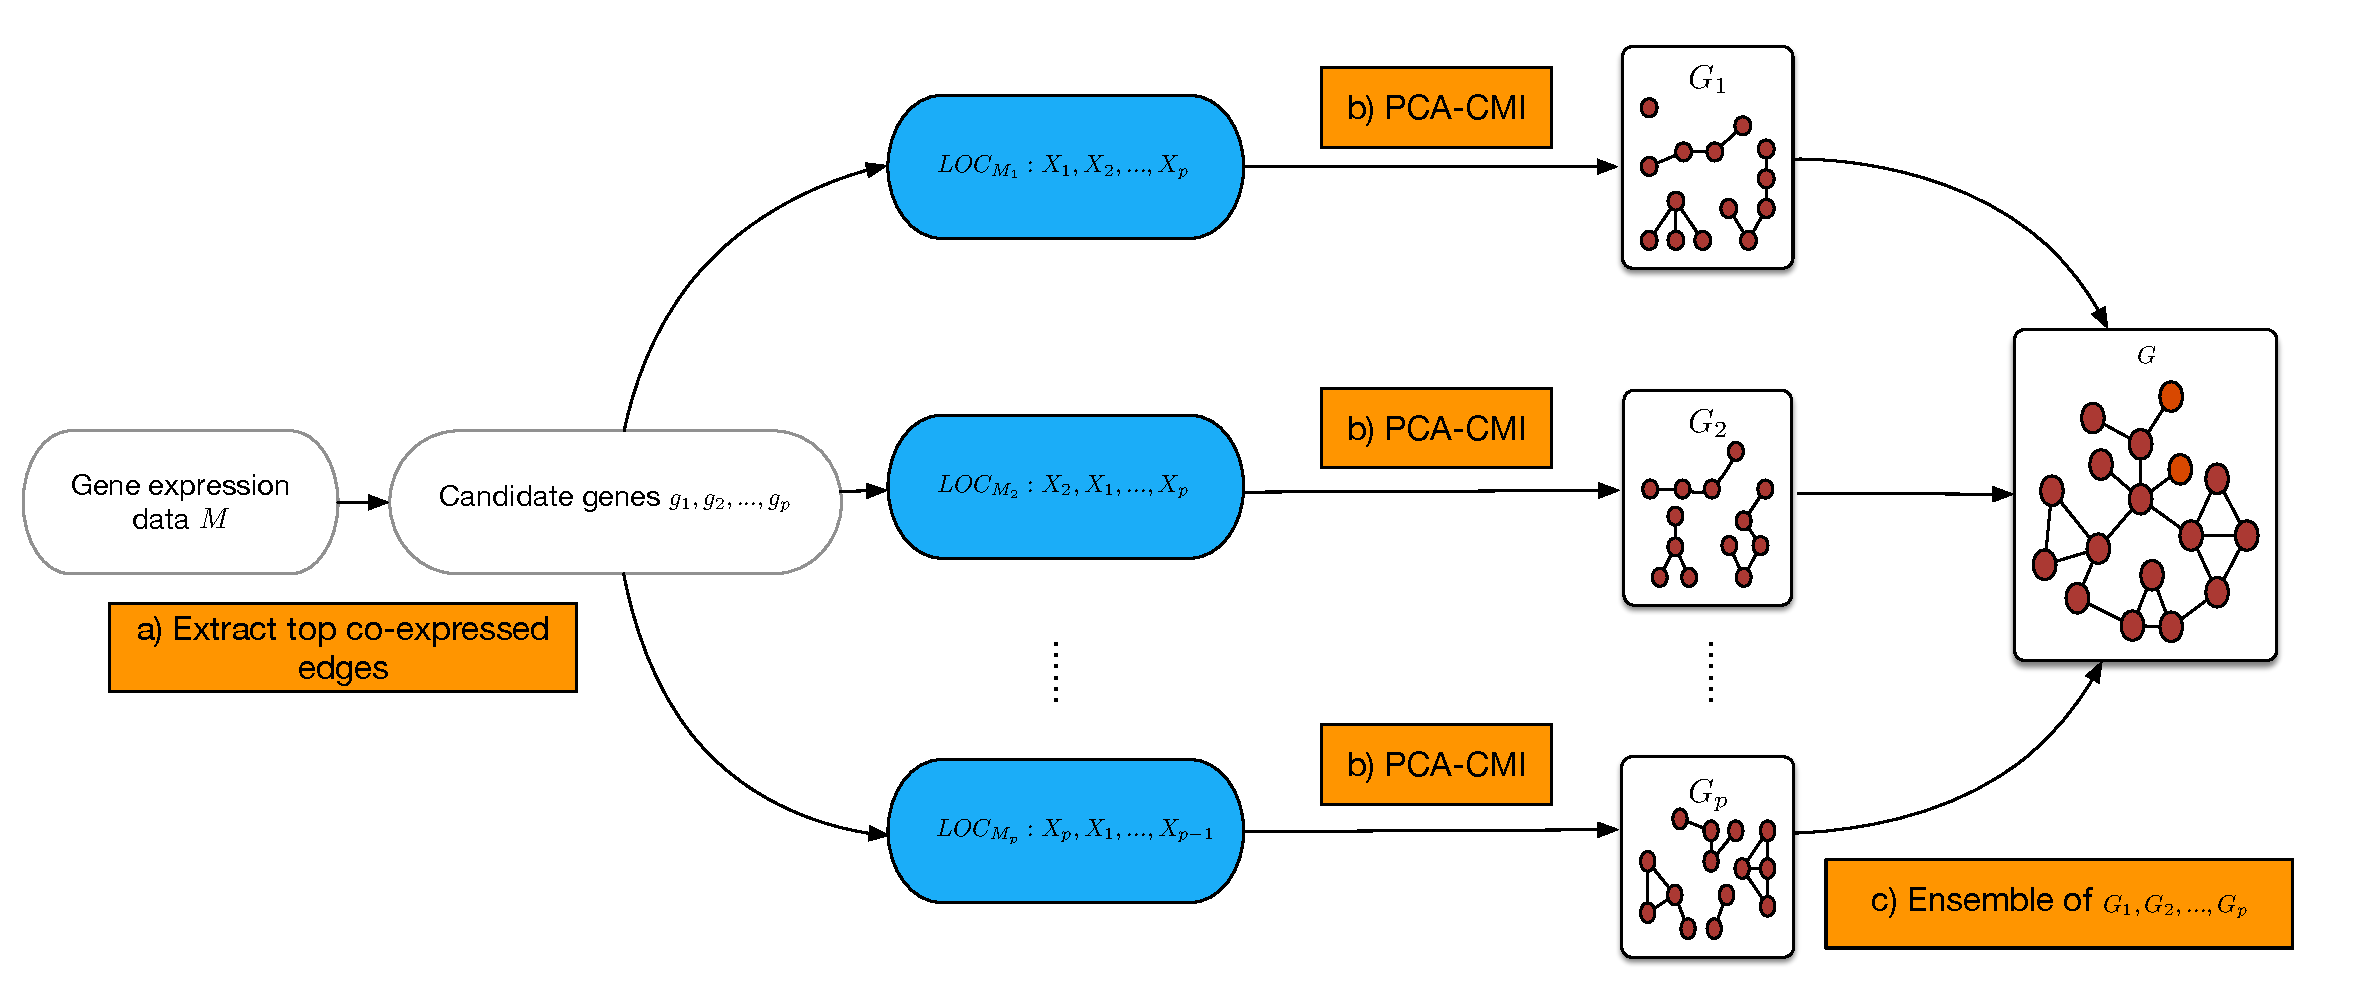
\includegraphics[width=0.95\textwidth]{pca-cmi-framework.pdf}
    \caption{Loc-PCA-CMI~方法框架图.
     a) 从基因表达矩阵~$M$~中抽取~top~$n$~条共表达边,其对应的候选基因为~$g_1,g_2,\ldots,g_{p}~$。
    这些候选基因被分组到局部簇中~$LOC_{M_1},~LOC_{M_2},\ldots,LOC_{M_{p}}$,
    其中~$g_1,g_2,\ldots,g_{p}$~是分别作为每个簇的质心。
    b) 对每一个局部之间有重叠的簇,我们应用~PCA-CMI~算法来得到它准确的结构。
    c) 聚合~$G_1,~G_2,~\ldots,~G_p$~来得到~GRN~的最终结构图~$G$。
    }
    \label{pca-cmi-fr}
\end{figure}

\begin{algorithm}[!htbp]
    \caption{Loc-PCA-CMI~伪代码} %?????
    \label{alg}
    {\bf Input:} %?????? \hspace*{0.02in}??????????? \\ ????
    $M$ (the gene expression data matrix), $m$ (the number of genes), $n$ (the number of top ranked edges), $c$ (constant number); $k$ (CMI order number) and $\beta$ (order threshold) in subroutine PCA-CMI.
    
    {\bf Output:} %???????
    Graph weight matrix $G$ 
    %\begin{spacing}{1.5}
    \begin{algorithmic}[1]
    \If {$m \leq c$} 
    \State $G$ $\leftarrow$ PCA-CMI$(M, k, \beta)$;
    \State \Return $G$
    \Else
    \State Construct pair-wise gene-gene Pearson correlation matrix $\Omega = \rho(M_i, M_j)$;
    \State Select top $n$ edges as $E$ with highest Pearson correlation value in $\Omega$ with FDR correction in p-value, and according to which to get 
    $p$ candidate genes as $g_1,g_2,\ldots,g_{p}$;
    \For{each gene in $g_1,g_2,\ldots,g_{p}$} 
      \State Retrieve its directly connected genes that in edges list $E$ as local cluster $LOC_{M_i}$;
    \EndFor
    \For{each cluster $LOC_{M_i}$  in $LOC$}
      \State $G_{i}$ $\leftarrow$ PCA-CMI$(LOC_{M_i}, k, \beta)$;
    \EndFor
    \State $G$ $\leftarrow$ mean$(G_{1},G_{2},\ldots,G_{p})$;
    \State \Return $G$
    \EndIf
    \end{algorithmic}
    %\end{spacing}
\end{algorithm}

算法~\ref{alg}~的计算复杂度通常由两个因素决定:~第一个是局部重叠簇~$p$~的数量,通常低于基因数~$m$; 第二个是~PCA-CMI~子程序的复杂性。
~PCA-CMI~的计算复杂度由~CMI~阶数~$k$~和~$LOC_{M_i}$~的簇大小~$|C|$~控制,可以粗略估计为~$O(|C|^k)$~。
因此,~PCA-CMI~的最终计算复杂度可以计算为~$O(m *|C|^k)$。
在最坏的情况下, 如果簇大小~$|C|$~等于~$m$, 即每个簇包含其中的所有基因, 因此计算复杂度为~$m*m^k = m^{k+1}$。 
然而, 这种最糟糕的情况在实验中很少发生, 因为~$|C|$~通常低于~$m$。
另外, 在实际运行中, 所有~PCA-CMI~子程序可以并行执行, 以使所提出的算法~Loc-PCA-CMI~更快地结束。

\subsection{数据集}

我们使用来自著名的~DREAM3~竞赛的六个模拟数据~\cite{schaffter2011genenetweaver}~对~Loc-PCA-CMI~的性能进行了基准测试。
~DREAM3~使用~GeneNetWeaver~软件来模拟生成基因网络表达数据。
在来自已知生物模式的调节相互作用系统的子网:~Ecoli~(大肠杆菌)~和~Yeast~(酵母)~的基础上,
得到测试使用的基准网络。 
在我们的实验中评估了~DREAM3~中的总计六个基因敲除表达网络,
其包括三种不同规模的网络节点数:~10,~50,~100, 和两种不同类型的生物:~Ecoli~和~Yeast。

表~\ref{tbl}~展示了这~6~个数据集的详细描述。
\begin{table} [!htbp]
%\caption{Descriptions of the datasets in our experiments}
\caption{实验所使用的数据集描述} 
\label{tbl} 
\begin{center}
\resizebox{\columnwidth}{!}{%
\begin{tabular} {cccccc} 
\toprule
Datasets  & Number of samples & Average(Max) degree & Number of edges & Network density \\ 
\midrule
DREAM3-10 Ecoli &11 & 2.2(5) & 11 & 0.244\\
DREAM3-50 Ecoli & 51 & 2.48(14) & 62 & 0.051\\
DREAM3-100 Ecoli & 101 & 2.5(14) & 125 & 0.025\\
DREAM3-10 Yeast &11 & 2(4) & 10 & 0.222\\
DREAM3-50 Yeast & 51 & 3.08(13) & 77 & 0.063\\
DREAM3-100 Yeast & 101 & 3.32(10) & 166 & 0.034\\
\bottomrule
\end{tabular}
}
\end{center}
\end{table} 

针对每个数据集而言,输入数据文件中的行代表样本~(实验),~列代表基因~(实验变量)。
第一行是野生型表达数据,该样本中的每个基因都保持稳定状态。
第~$l$~($l>1$)~行则表示在对应的样本中第~$l-1$~个基因敲除后其它基因的表达量。

\subsection{结果和讨论}

如算法~\ref{alg}~中所述,三个参数会影响方法~Loc-PCA-CMI~的性能。
第一个参数是选定的~top~边的数目~$n$,
如果~$n$~增加,则考虑更多边,随后局部簇大小将增加。
第二个参数是~$\beta$,它作为~MI~和~CMI~的阈值来决定独立性。
第三个参数是~CMI~阶数~$k$,从理论上讲,通过增加~$k$,如果~CMI~没有达到~$k-1$~阶的阈值~$\beta$,结构会更准确。
第二个和第三这两个参数也是~PCA-CMI~和~PCA-PMI~里面的参数。
$n$~的最佳值可以通过交叉验证获得,通常~$n$~的较大值可以促成更大规模的群集,并且网络中涵盖更多基因;
在我们的实验中,我们将其值均匀地设置为~$n =\binom{m} {2}/5$。
除了上述三个参数外,我们在算法~\ref{alg}~中设置常量~$c = 10$,
即如果基因数小于或等于~10,则~Loc-PCA-CMI~直接称为~PCA-CMI,
并且在这种情况下,~Loc-PCA-CMI~和~PCA-CMI~的性能是相同的。
我们通过评估接收器工作特性曲线下面积~(AUROC)~和准确率召回率曲线下面积~(AUPR)~来评估~Loc-PCA-CMI~的性能。
与稀疏生物网络一样,不存在的边~(负样本)~的数量明显超过现有边~(正样本)~的数量; 
事实上,~AUPR~对~AUROC~\cite{saito2015precision}~提供了更多信息。
我们倾向于使用~AUPR~进行评估,但为了与采用~AUROC~作为评估指标的其它方法进行保守比较,
我们还将~AUROC~作为补充指标。
较高的~AUROC~和~AUPR~值表明更准确的~GRN~预测。
为此,我们通过比较黄金标准网络中的监管边与最高~$q$~边来计算真阳性~(TP)、真阴性~(TN)、假阳性~(FP)和假阴性~(FN)边的数量来自~Loc-PCA-CMI~的排名列表输出。
通过绘制真实阳性率~TPR = TP/(TP + FN)~与假阳性率~FPR = FP/(FP + TN)~来增加~$q$~($q = 1, 2, \ldots, m^2$)来构建~ROC~曲线。
类似地,绘制精度~(TP/(TP+FP))~和召回~(TP/TP+FN)曲线以增加~$q$。
应该注意的是,在算法~\ref{alg}~中,在获得每个局部聚类之后,~PCA-CMI~和~PCA-PMI~都是后续结构精炼化的候选方案。
类似地,如果用~PCA-PMI~替换~PCA-CMI,则会生成一种新方法,我们将其命名为~Loc-PCA-PMI。
然后得到四种基于~PCA~(路径一致性)~的方法,包括~PCA-PMI、PCA-CMI、Loc-PCA-PMI和~Loc-PCA-CMI,
所有这些方法目前都属于无模型~(model-free)~方法。
如表~\ref{tbl}~所示,在六个基准数据集~DREAM3-10~中,~Ecoli~和~Yeast~数据集仅包含~10~个基因,
因此根据算法~\ref{alg}~的原理,
Loc-PCA-CMI~和~PCA-CMI~的表现相同,就像~Loc-PCA-PMI~和~PCA-PMI~的情况一样。
为了对这些基于~PCA~(路径一致性)~的方法进行有意义的比较,
我们选择了其它四个基因数大于~10~的数据集。
阶数在~\cite{zhang2011inferring,zhao2016part}~中有所讨论,
我们在实验中设置~$\beta = 0.03$,~$k = 2$。
同时为了探讨阶数~$k$~的大小是如何影响这些方法的性能,
在固定阈值~$\beta = 0.03$~后,我们把这四种方法中的阶数~$k$~从~1~逐渐变化为~10,
然后分别计算~AUROC~和~AUPR。
图~\ref{fig:k}~总结了基准数据集的结果, 我们可以从此图得到以下两个结论:
\begin{itemize}
    \item 阶数~$k$~会对这四种基于~PCA~的方法的结果产生影响,通常当~$k$~达到~4~时~AUPR~和~AUROC~变得稳定,除了~DREAM3-100 Ecoli数据集上略有不同。
    \item Loc-PCA-CMI~和~Loc-PCA-PMI~分别比~PCA-CMI~和~PCA-PMI~产生更高的~AUPR~和~AUROC,
    因此该算法采用的局部聚类策略有助于提高方法~PCA-CMI~和~PCA-PMI~的表现。
\end{itemize}

  \begin{figure*}[!htbp]
    \centering
    \begin{minipage}[b]{0.45\linewidth}
      \centering
      \centerline{
        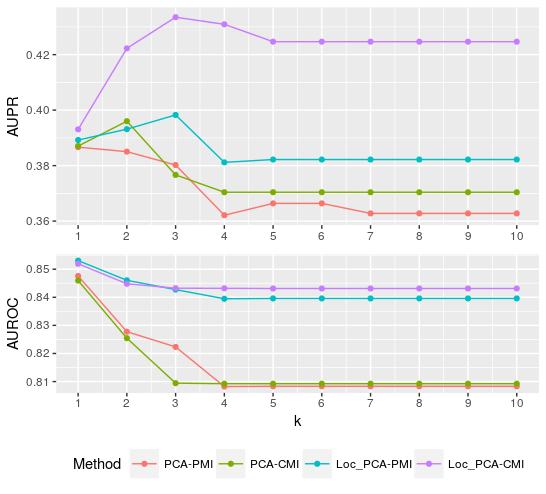
\includegraphics[width = \linewidth]{K_Dream50_Ecoli.png}}
      \centerline{(A) DREAM3-50 Ecoli}
      \medskip  
    \end{minipage}
    \begin{minipage}[b]{0.45\linewidth}
      \centering
      \centerline{
        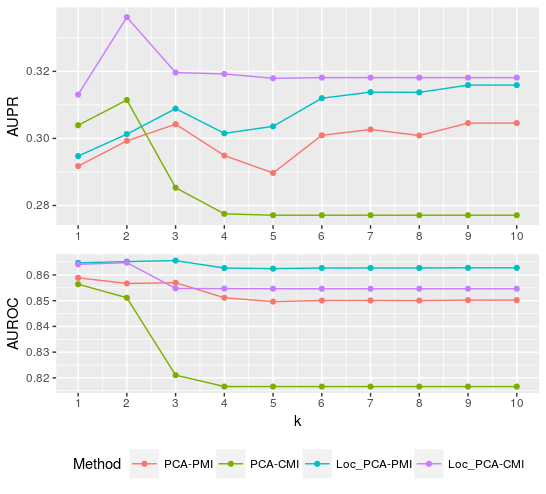
\includegraphics[width =\linewidth]{K_Dream100_Ecoli.png}}
      \centerline{(B) DREAM3-100 Ecoli}
      \medskip  
    \end{minipage}
      \begin{minipage}[b]{0.45\linewidth}
      \centering
      \centerline{
        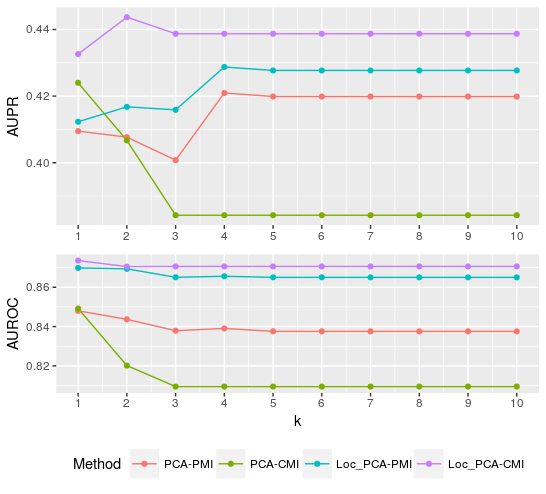
\includegraphics[width = \linewidth]{K_Dream50_Yeast.png}}
      \centerline{(C) DREAM3-50 Yeast}
      \medskip  
    \end{minipage}
    \begin{minipage}[b]{0.45\linewidth}
      \centering
      \centerline{
        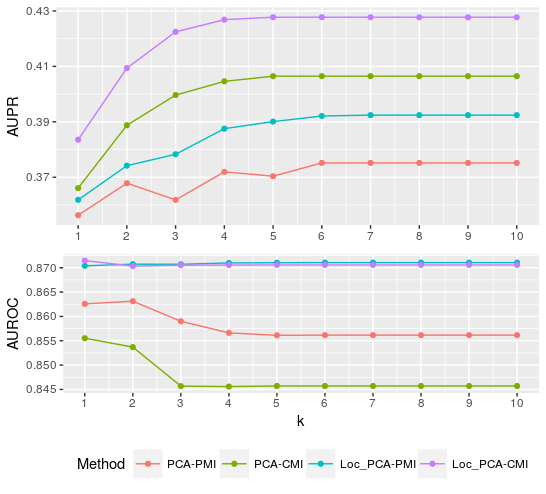
\includegraphics[width =\linewidth]{K_Dream100_Yeast.png}}
      \centerline{(D) DREAM3-100 Yeast}
      \medskip  
    \end{minipage}
    \caption{%AUPR and AUROC  by varying $k$ from 1 to 10 of four PCA based methods on four different datasets: 
    通过在四个不同的数据集上~k~从~1~改变到~10, 基于~PCA~(路径一致性)~的四个算法的~AUPR~和~AUROC~结果示意图。
    (A) DREAM3-50 Ecoli; 
    (B) DREAM3-100 Ecoli; 
    (C) DREAM3-50 Yeast; 
    (D) DREAM3-100 Yeast。}
    \label{fig:k}
    \vspace{-0.5em}
  \end{figure*}

我们在六个基准数据集上使用~Loc-PCA-CMI~和四种基准方法~ARACNE、MRNET、PCA-PMI、PCA-CMI~进行了比较实验。
我们使用~R~包~``minet" 和其默认参数来评估~ARACNE~和~MRNET~\cite{meyer2008minet}。
使用~Pearson~相关系数直接从连续基因敲除表达数据~\cite{olsen2008impact,meyer2010information}~中近似估计方法的~MI~矩阵。
为了实现~PCA-PMI~和~PCA-CMI, 我们根据~\cite{zhang2011inferring,zhao2016part}~中提供的~URL~下载了~MATLAB~代码。
另外,~PCA-PMI~和~PCA-CMI~方法中的参数使用它们推荐的默认值,也就是~$\beta = 0.03$~和~$k = 2$。
对于~Loc-PCA-CMI, 我们还对这两个参数采用了相同的值进行比较。
表~\ref{tab:performance_comparison}~给出了实验结果的~AUROC~和~AUPR。
从表中可以看出,当网络规模增大时, 所有的方法的~AUPR~都会急剧下降。
Loc-PCA-CMI~仅在~DREAM3-10~Yeast~数据集中的~PCA-PMI~(或本文提出的~Loc-PCA-PMI~)之后,
而在其它五个数据集中,就~AUROC~和~AUPR~而言,
Loc-PCA-PMI~表现优于其它四种方法~ARACNE、MRNET、PCA-PMI~和~PCA-CMI。
此外,为了更完整地比较,我们还在表中展示了~Loc-PCA-PMI~的实验结果,
其中~$\beta = 0.03$~和~$k = 2$。
Loc-PCA-CMI~和~Loc-PCA-PMI~在~AUROC~上几乎相同。
然而,在大多数数据集中,~Loc-PCA-CMI~的~AUPR~优于~Loc-PCA-PMI。
我们提供了包括所有方法、基准数据集和测评脚本相关的资料, 
在~\url{https://github.com/chenxofhit/Loc-PCA-CMI.git}~上获取。

\begin{table}[!htbp]
    % \scalebox{0.9}{
    % \begin{minipage}{1.1\linewidth}
    \resizebox{\columnwidth}{!}{%
      \centering  
      \begin{threeparttable}  
      %\caption{AUROC and AUPR for the six datasets using different methods}  
      \caption{使用不同方法在六个数据集上的~AUROC~和~AUPR~结果}  
      \label{tab:performance_comparison} 
        \begin{tabular}{ccccccccccccc}  
        \toprule  
        \multirow{2}{*}{Dataset}&  
        \multicolumn{2}{c}{ARACNE}&\multicolumn{2}{c}{MRNET}&\multicolumn{2}{c}{PCA-PMI}&\multicolumn{2}{c}{Loc-PCA-PMI}&\multicolumn{2}{c}{PCA-CMI}&\multicolumn{2}{c}{Loc-PCA-CMI}\\
        \cmidrule(lr){2-3} \cmidrule(lr){4-5}  \cmidrule(lr){6-7}  \cmidrule(lr){8-9}  \cmidrule(lr){10-11}  \cmidrule(lr){12-13} 
        &AUROC&AUPR &AUROC&AUPR &AUROC&AUPR &AUROC&AUPR &AUROC&AUPR &AUROC&AUPR\\
        \midrule  
        DREAM3-10 Ecoli  & 0.523 &0.255   &0.518&0.258    &0.816&0.483    &0.816&0.483    &{0.825}&{0.499}   &\textbf{0.825}&\textbf{0.499}\\
        DREAM3-50 Ecoli  &0.474 &0.050    &0.529&0.061    &0.828&0.385    &\textbf{0.846}&0.393    &0.825&0.396 &0.845&\textbf{0.422}\\
        DREAM3-100 Ecoli &0.505&0.027     &0.488&0.025    &0.857&0.299    &0.865&0.301    &0.851&0.311       &\textbf{0.865}&\textbf{0.336}\\
    
        DREAM3-10 Yeast  &0.628&0.321     &0.644&0.322    &0.995&0.933    &\textbf{0.995}&\textbf{0.933} &0.993&0.918 &0.993&0.918\\
        DREAM3-50 Yeast  &0.507&0.074     &0.524&0.080    &0.844&0.408    &0.869&0.417 &0.820&0.406   &\textbf{0.871}&\textbf{0.444}\\
        DREAM3-100 Yeast &0.547&0.040     &0.556&0.042    &0.863&0.368    &\textbf{0.871}&0.374 &0.854&0.389   &0.870&\textbf{0.409}\\
        \bottomrule  
        \end{tabular}  
        \end{threeparttable}  
        %   \end{minipage}
        %   }
        }
    \end{table} 

\subsection{结论}
我们基于从局部结构出发然后合并局部构造全局网络的想法,提出了一种命名为~Loc-PCA-CMI~的新的基于无模型~(model-free)~的~GRN~结构推断方法。
与~PCA~类算法~top-down~的思想相反,~Loc-PCA-CMI~采用了类似~bottom-up~的策略。
在~DREAM3~敲除数据集上的实验表明,~Loc-PCA-CMI~受益于局部聚类的策略。
此外,~Loc-PCA-CMI~优于其它方法,
包括~ARACNE、MRNET、PCA-PMI~和~PCA-CMI,特别是在大小为~50~和~100~的网络上表现更佳。

Loc-PCA-CMI~在处理局部网络结构的时候引入了~PCA-CMI,其计算效率的局限性也会受~PCA-CMI~的限制,
特别是在处理大型数据集时。
因为在大型网络的情况下, 局部簇的数量可能会非常大。
但是,如果我们可以控制每个局部簇的大小,我们的方法也将适用于大型数据集。
我们未来的工作之一是改进聚类策略,
例如整合蛋白质复合物~\cite{li2017identification, li2017dynetviewer},
以便更有效地处理大规模样本数据。
另外,值得注意的是,我们主要关注推断~GRN~的结构,并没有考虑网络自身的稳定性问题。
因此,我们未来的研究将尝试从网络稳定性的角度出发推断更鲁棒的基因调控网络结构。

\newpage
\section{基于数据驱动和抽样的 GRN 构建方法}
\label{sec:d3grn}

\subsection{引言}

% 从基因表达数据构建基因调控网络 (GRNs) 是系统生物学中一个具有挑战性的基础问题。
在上一章中, 本文提出了一种基因调控网络的结构构建方法,
Loc-PCA-CMI 输出的是无向网络, 基因和基因之间的权重表示的是调控相互作用关系的强弱。
很多情况下在 GRN 中,除了关注基因之间的相互作用之外,还对基因调控的具体方向十分感兴趣。
为了构建有向网络,现有的一些流行的算法将 GRN 构建表述为回归问题,并以聚合 (ensemble) 策略获得最终的网络。
最近关于数据驱动的动态网络构建的研究,主要是偏微分方程和机器学习相结合的方法, 
为本文利用回归方法研究基因调控网络提供了一个全新的视角。
在本章的研究中,我们提出了一种改进 ARNI 的数据驱动和抽样的动态网络构建方法来构建基因调控网络,命名为 D3GRN。
该方法将每个目标基因的调控关系转化为函数分解问题,
利用改进的揭示网络相互作用的算法 ARNI 来构造以目标基因为中心的局部基因调控网络。
本文采用抽样 (bootstrapping) 和基于面积的评分方法 (area-based scoring) 来构建最终的全局网络,
克服了 ARNI 仅从单个节点构建局部网络的缺陷。
实验结果表明,在 DREAM4 和 DREAM5 基准数据集上, D3GRN 在 AUPR 评价指标上优于其它最先进的算法。

\subsection{相关工作}

在 DREAM 系列挑战赛的推动下,大量研究人员采用机器学习回归模型对基因调控网络进行构建。
这类方法本质上可以看作是关联网络模型的延伸,
不同的是,关联网络只关注量化相互作用,回归方法则能推断出基因之间的相互作用方向。
回归模型将基因调控建模转化为机器学习特征选择的问题,
也就是将目标基因的表达看作是调控基因表达之间的相互线性作用或者非线性作用的结果,
然后结合 bagging 或者 boosting 的思想,构建出最终的基因调控网络。
GENIE3 \upcite{huynh2010inferring} 被认为是在一些基准数据集的最好方法 \upcite{marbach2010revealing},
该方法是基于随机森林训练了一个回归模型,为每个基因挑选出最重要的调控因子。
在 GENIE3 基础上, GRNBoost2 \upcite{moerman2019grnboost2} 做了扩展, 更适合于有成千上万个基因的大规模数据集。
所不同的是,它是通过使用随机梯度增强的机器学习回归方法来进行特征选择, 
并加入正则化和``early stop" 机制来防止模型过拟合。 
TIGRESS \upcite{Haury2012} 使用最小角回归 (LARS) 并结合稳定性选择来解决 GRN 的构建问题。
NIMEFI \upcite{ruyssinck2014nimefi} 研究了合并几种特征选择方法的潜在效果,
例如 GENIE3, 集成支持向量回归 (E-SVR)和 集成弹性网络 (E-EL) \upcite{zou2005regularization},
并在一般框架下结合这些方法对最终的基因调控网络进行预测。
bLARS \upcite{singh2016blars} 可以视为 TIGRESS 的变种方法,
其中调控关系是从预定义的基函数建模取得的,并且通过修改的 LARS 算法构建出最终的 GRN。

最近几年尤其是在物理领域中,数据驱动的动态网络构建是一个非常有吸引力的课题。
SINDy \upcite{brunton2016discovering} 假设只有少数重要变量可以控制动态系统,
因此,偏微分方程在潜在的函数空间中是稀疏的。
然后,它使用稀疏回归来准确确定表示数据所需要的动态控制方程中的少数项。
ARNI \upcite{casadiego2017model} 是一个独立于模型的框架,依赖于它们的非线性聚合动力学, 
来推断网络动态系统中的直接交互作用。
与 SINDy 不同的是, ARNI 在最终实现的时候是通过函数分解和基函数的展开来求解非线性微分方程组。

虽然 bLARS, SINDy 和 ARNI 是在不同的研究领域提出来的,
它们的基本思想十分相似。
本文从三个不同的方面对这三个方法进行比较, 如表 \ref{comparision} 所示。
形式化函数分解 (formal function  decomposition) 意味着该方法是否具有函数分解方程的形式描述;
稀疏组约束 (sparse group  constraints ) 指示该方法是否利用候选项的稀疏组约束,
而基于网络的构造 (network based construction) 表明该方法是否能重建整个网络结构。
 SINDy 和 ARNI 都没有解决从网络层面发现物理机制的问题,它们仅侧重于以某一个特定节点为目标节点然后构建局部的网络。
由于目前还没有一种方法能覆盖​​这三个方面,
所以本文第一次综合考虑这三个方面,提出了一种改进的数据驱动的动态网络构建方法。
 D3GRN 将每个目标基因的调控关系转化为函数分解问题并通过采用改进的 ARNI 算法,
来构造每个目标基因相互作用的候选基因及其局部 GRN 结构。
最后,本文采用基于面积的评分方法聚合经过抽样之后得到的 GRN 网络,来构建最后的 GRN 有向网络。
在 DREAM4 和 DREAM5 基因调控网络重建挑战赛数据集上, 本文将 D3GRN 与其它几种当今表现最好的有向基因调控网络构建方法进行了比较,
结果表明 D3GRN 在 AUPR 上具有优势。

\begin{table}[!htbp]
    %\caption{Comparison of the related methods}
    \caption{相关方法比较}
    \centering
%    \begin{adjustbox}{max width=0.5\textwidth}
    \label{comparision}  
    \begin{tabular}{lccccc}
    \toprule
    &bLARS &SINDy&ARNI&D3GRN\\
    \midrule
    形式化函数分解 &$\times$ &\checkmark &\checkmark&\checkmark\\ 
    稀疏组约束 &\checkmark &$\times$ &\checkmark&\checkmark\\
    基于网络的构造&\checkmark&$\times$ &$\times$&\checkmark\\
    \bottomrule                   
    \end{tabular}
  %  \end{adjustbox}
\end{table}

\subsection{GRN 构建方法 D3GRN}
% \subsubsection{问题定义}

如果不考虑基因之间的上游或下游调节关系并且忽略自我调节机制,则可以将 GRN 视为有向无环图 (directed acyclic graph, DAG)。
在 DAG 中,每个节点对应于基因,每条边代表基因之间的调节关系。
和许多其它聚合方法一样 (例如 \upcite{huynh2010inferring,Haury2012,slawek2013ennet,ruyssinck2014nimefi,guo2016gene,zheng2019ensemble}),
它不利用不同实验条件的信息 (例如基因敲除,扰动甚至重复),
我们仅基于基因表达数据使用 GRN 推理问题的通用框架。
作为输入基因表达数据,本文考虑在 $M$ 实验条件下测量 $N$ 基因的表达量。
因此,基因表达数据 $A$ 定义如下:
\begin{equation}
\label{eq:definion}
A = [x_1,x_2,\ldots,x_N] \in \mathbb{R} ^ {M \times N}
\end{equation}
其中 $x_i$ 是所有 $M$ 实验条件中第 $i$ 个基因的表达值的列向量。

GRN 构建方法预测基因表达数据基因之间的调节关系 $A$。
大多数方法提供了从最高到较低置信度 (confidence) 的潜在调控关系,
也就是 (source gene $i$, target gene $j$, confidence) 的排序列表。
随后可以通过在该排序列表上使用变化的 confidence 阈值来获得不同的 DAG。
因为最终用户可以自由探索各个阈值所对应的网络 \upcite{slawek2013ennet},
本研究中我们只关注列表里面具体的排序先后问题。
事实上,排序是 DREAM \upcite{stolovitzky2007dialogue} 挑战赛的标准预测格式,
各种 GRN 构建方法最终都是通过提交其输出的排序列表文件到 DREAM 联盟进行评比。
此外,跟上一章我们提出的 Loc-PCA-CMI 方法类似,我们也不考虑排序列表表示的网络的稳定性。
为了从表达数据 $A$ 构建出调控网络,
本文计算一个权重分数 $S_{ij}$, 也就是列表每一个元素中的 confidence,
表示基于基因表达水平值上基因 $i$ 调控基因 $j$的强度 (包括上调和下调)。

% \subsubsection{基于集成回归方法的网络推理}

受基于特征选择的集成方法,例如 GENIE3 \upcite{huynh2010inferring} 和 TIGRESS \upcite{Haury2012} 成功被应用的启发,
$n$ 个基因的 GRN 构建问题可以分解为 $n$ 个子问题,
其中每个子问题都可以看作是机器学习中的特征选择问题 \upcite{nasrabadi2007pattern}。
更具体地说,对于每个目标基因,本文希望从基因表达水平上确定直接影响它的基因子集。
设 $A$ 是等式 (\ref{eq:definion}) 中定义的基因表达数据,
第 $i$ 个基因为目标基因,本文在 $M$ 个实验条件 (即样本) 下定义了其它候选表达调控因子:
\begin{equation}
  \label{eq:x}
  x^{-i} = [x_1,\ldots,x_{i-1},x_{i+1},\ldots,x_N]
  \end{equation}

特征选择问题可以表示为:
\begin{equation}
\label{eq:fs}
x_i =  F(x^{-i}) + \epsilon , \forall i \in \{1,2,\ldots,N\}
\end{equation}
其中, $F$ 是任意一个平滑, 典型的如 $x^{-i}$ 个基因 (也就是跟基因 $i$ 相关的基因) 表达值的非线性函数; $\epsilon$ 是噪声项 \upcite{huynh2010inferring,Haury2012}。
% Generally, the function $F$ is unknown which can be defined indirectly as:
% \begin{equation}
% \label{eq:ffunction}
% F(x^{-i}) = \sum_{1}^{n} w_{ji}x_j , \forall j \in \{1,\ldots,i-1,i+1,\ldots,n\}
% \end{equation}
% where $w_{ji}\geqslant 0$ represents the strength (or confidence) that gene $i$ associates (i.e., regulates) gene $j$. 
% The rankings of the regulatory links of gene $i$ is obtained by computing the $w_{ji}$.
把 $N$ 个独立的基因排序聚合起来,我们能得到一个全局的 GRN 的调控关系的排序。

% \subsubsection{使用 D3GRN 进行 GRN 推断}

整个方法流程如图 \ref{d3grn} 所示,实现细节如算法 \ref{alg:D3GRN} 所示。
其中, $A_j$ 指的是矩阵 $A$的第 $j$ 列, $A_I$ 是 $A$ 中包含索引列集合 $I$ 的子矩阵。
假定,输入的基因表达矩阵 $A \in \mathbb{R}^{M \times N}$, 
并且转录因子的索引 $I \subset \{1,\ldots,N\}$, 
同时抽样次数和 ARNI 算法的步数 $L$ 已经知道。
在 $A$ 中放回重复抽样,针对第 $i$ 次抽样,对于每一个目标基因 $j$, 
对应的目标基因 $j$ 的表达值为 $y$, 
其它的转录因子 $X$ 的表达值也被获取到。
ARNI 算法调用后,返回的是被选中的调控因子 $SM_j$ 的一个有序列表 (ordered list)。
最后,在所有的 $b$ 轮抽样结束后,
矩阵 $SM$ 作为输入变量,通过基于面积的评分方法,
本文赋予一个候选的转录因子和目标基因之间的边 0 和 1 之间的得分。
抽样和基于面积的评分方法的细节,以及计算复杂度分析,
本文在后续的章节中会详细介绍。
 
\begin{figure}[!htbp]
  \centering
  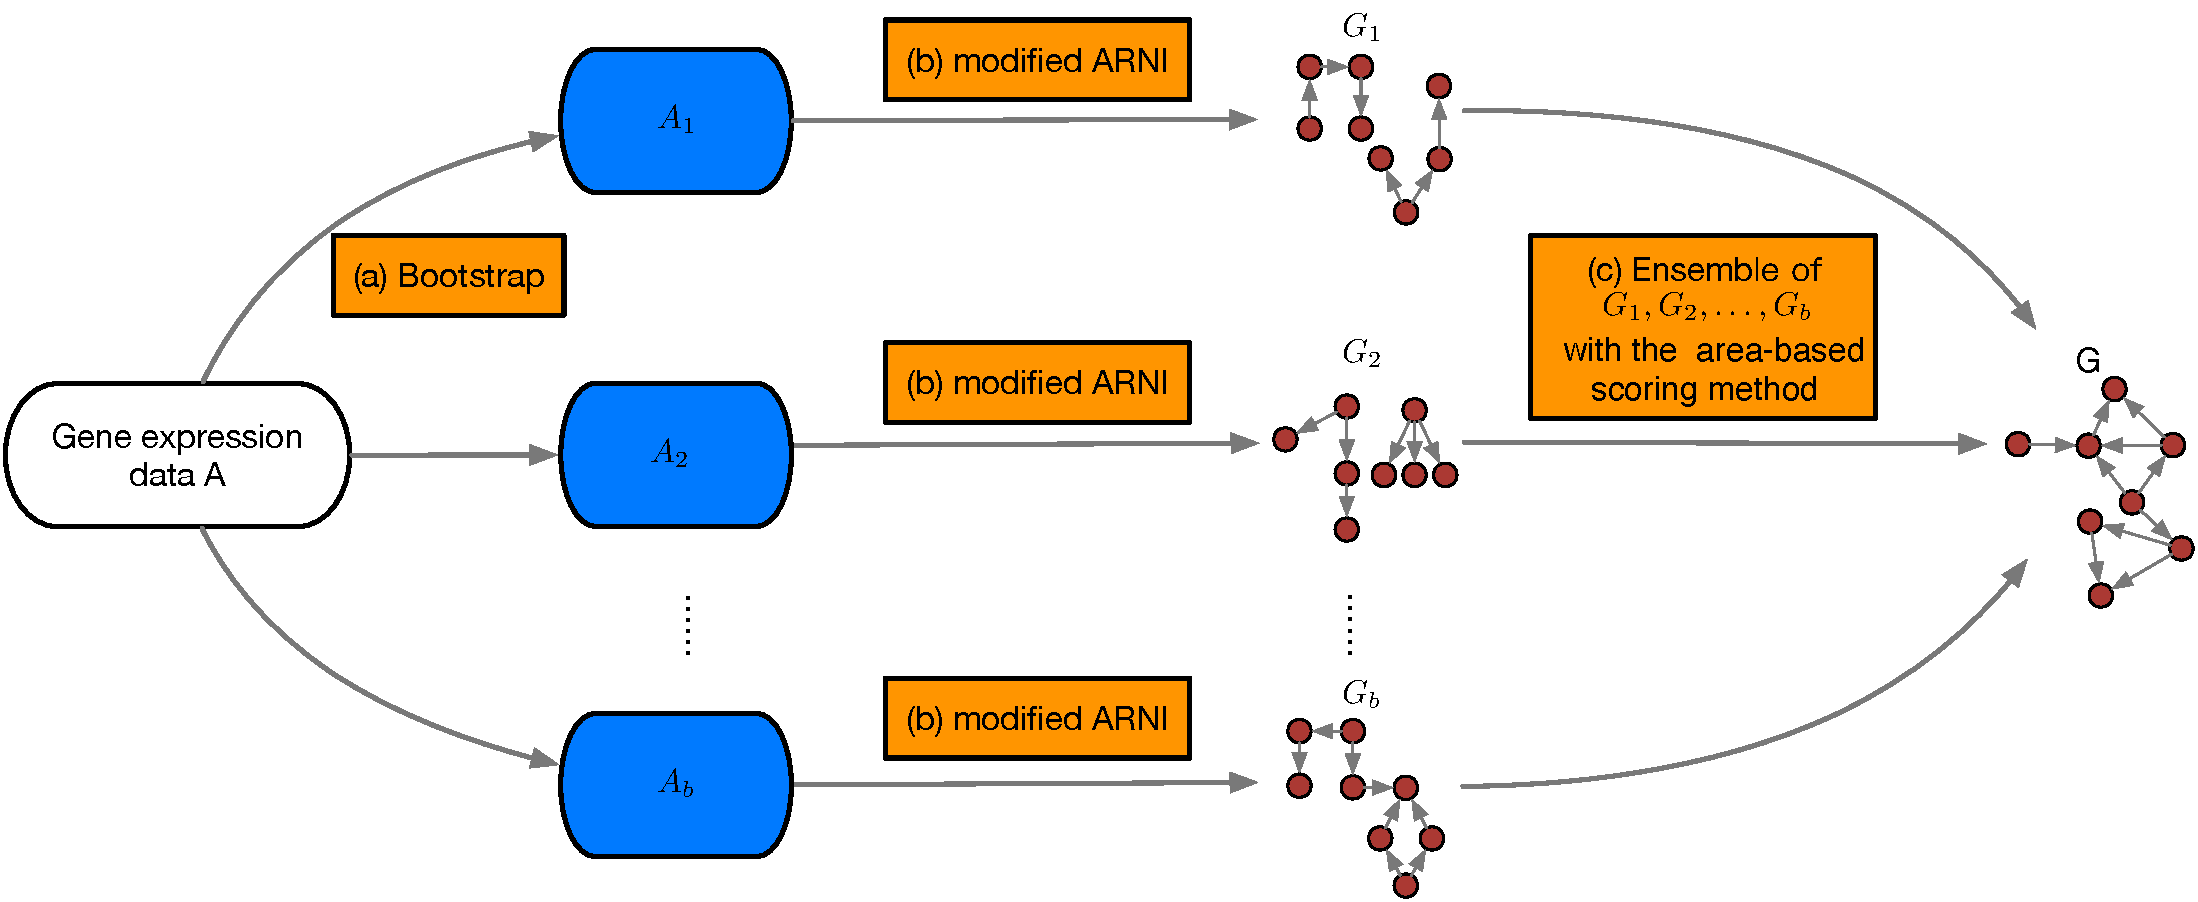
\includegraphics[width=0.95\textwidth]{d3grn-framework.pdf}
  \caption{D3GRN 方法框架图。
  (a) 从基因表达矩阵 $A$ 中抽取 $b$ 轮放回重复抽样,分别得到 $A_1,A_2,\ldots,A_{b}$ 基因表达矩阵。
  (b) 对每一个抽样之后的表达样本,本文利用改进后的 ARNI 算法来得到它对应的 GRN。
  (c) 按照基于面积的评分策略聚合 $G_1, G_2, \ldots, G_b$ 来得到 GRN 的最终结构 $G$。
  }
  \label{d3grn}
\end{figure}

\begin{algorithm}
  %\caption{D3GRN Pseudo Code}
  \renewcommand{\thealgorithm}{3-1}
  \caption{D3GRN 方法伪代码}
  \label{alg:D3GRN}
  \begin{algorithmic}[1]
  \Require  $A \in \mathbb{R}^{M \times N}$, $I \subset \{1,\ldots,N\}$, 
            $|I| = n$,
            $b$ (the number of bootstrapping runs), $L$ (ARNI steps) %\Comment{Number of bootstrapping runs and ARNI steps}
  \Comment{$M$ samples, $N$ genes, I index set of $n$ regulators}
  
  \Ensure The score matrix $S$ 
  \State Initialize $S \in \mathbb{R}^{N \times n}$     \Comment{Initialize adjacency matrix of the GRN}
  \State Initialize $SM \in \mathbb{R}^{n \times b}$     \Comment{Initialize the selection matrix}
  \For{$i = 1 \to b$}                                   \Comment{For each bootstrapping run}
        \State $A^{*}$ = resample$(A)$                  \Comment{Resampling with replacement}
        \For{$j = 1 \to n$}                             \Comment{For each target gene}         
        \State $y = A^{*}_j, X = A^{*}_{I\setminus j}$
        \State $SM_{ji}$ = ARNI$(y,X,L)$                    \Comment{Returns selected tx-factors with the ARNI algorithm}
        \EndFor
  \EndFor           
  \State $S$ = area-score$(SM,L,b)$                      \Comment{Get the weight score matrix with the area-score metric}
  \State \Return $S$                                    \Comment{Output the score matrix}
\end{algorithmic}
\end{algorithm}

\subsubsection{局部 GRN 构建方法}

对于给定节点 $i$ 及其对应的微分方程, 
ARNI 转向获得网络中哪些节点 $j$ 之间有直接的物理相互作用,并出现在微分方程等式的右侧, 
而不是探索方程中这些节点之间的交互函数的细节。
具体地来说, 对于 $N$ 个节点的动态系统, 
ARNI 首先将节点 $i$ 的动态性分解为与网络中其它节点的交互项 \upcite{casadiego2017model}:
\begin{equation}
\label{eq:xi}
\begin{split}
% \dot{x_i}= & f_i(\Lambda ^i x)\\
%          = &\sum_{j=1}^{N} \Lambda^i_{jj} g^i_j(x_j) + 
%                              \sum_{j=1}^{N} \sum_{s=1}^{N}\Lambda^i_{jj}\Lambda^i_{ss}g^i_{js}(x_j,x_s)\\
%          + &\sum_{j=1}^{N} \sum_{s=1}^{N} \sum_{w=1}^{N}\Lambda^i_{jj}\Lambda^i_{ss}\Lambda^i_{ww}g^i_{jsw}(x_j,x_s,x_w)+ \ldots + \epsilon_{i}
% \end{split}
\dot{x_i}= & f_i(\Lambda ^i x)\\
         = &\sum_{j=1}^{N} \Lambda^i_{j} g^i_j(x_j) + 
                             \sum_{j=1}^{N} \sum_{s=1}^{N}\Lambda^i_{j}\Lambda^i_{s}g^i_{js}(x_j,x_s)\\
         + &\sum_{j=1}^{N} \sum_{s=1}^{N} \sum_{w=1}^{N}\Lambda^i_{j}\Lambda^i_{s}\Lambda^i_{w}g^i_{jsw}(x_j,x_s,x_w)+ \ldots + \epsilon_{i}
\end{split}
\end{equation}

其中 $\dot{x}_i :=[\dot{x}_{i,1}, \dot{x}_{i,2},\ldots,\dot{x}_{i,M}]\in \mathbb{R}^M$,
$f:\mathbb{R}^N \to \mathbb{R}$ 是一个平滑函数, 
对角矩阵 $\Lambda^i \in \{0,1\}^{N \times N}$ 中 $\Lambda^i_{j}=1$ 如果 $j$ 直接作用于 $i$, 
否则 $\Lambda^i_{j}=0$, $g^i_j:\mathbb{R} \to \mathbb{R}$, $g^i_{js}:\mathbb{R}^2 \to \mathbb{R}$, $g^i_{jsw}:\mathbb{R}^3 \to \mathbb{R}$,
并且一般 $g^i_{j_{1}j_{2}\ldots\\j_{K}}:\mathbb{R}^K \to \mathbb{R}$ 表示(未知)节点 $j_k$ ($k \in \{1,2,\ldots,K\}$) 和节点 $i$ 的第 $K$ 阶相互作用, 
最后一项 $\epsilon_{i}$ 代表于作用于 $i$ 的额外噪声。

函数 $g^i_{j_{1}j_{2}\ldots\\j_{K}}$ 无法显式访问 \upcite{casadiego2017model},可以将其分解为基函数 $h$,
本文可以将等式 (\ref{eq:xi}) 重写为:
\begin{equation}
\label{eq:xi_with_h}
\begin{split}
% \dot{x_i} =  &\sum_{j=1}^{N} \Lambda^i_{jj} \sum_{p=1}^{P_1} c^i_{j,p}h_{j,p}(x_j) \\
% + &  \sum_{j=1}^{N} \sum_{s=1}^{N}\Lambda^i_{jj}\Lambda^i_{ss} \sum_{p=1}^{P_2} c^i_{js,p}h_{js,p}(x_j,x_s) \\
%                              + &\sum_{j=1}^{N} \sum_{s=1}^{N} \sum_{w=1}^{N}\Lambda^i_{jj}\Lambda^i_{ss}\Lambda^i_{ww} \sum_{p=1}^{P_3} c^i_{jsw,p}h_{jsw,p}(x_j,x_s,x_w)\\
%                              + &\ldots + \epsilon_{i} 
% \end{split}
\dot{x_i} =  &\sum_{j=1}^{N} \Lambda^i_{j} \sum_{p=1}^{P_1} c^i_{j,p}h_{j,p}(x_j) \\
+ &  \sum_{j=1}^{N} \sum_{s=1}^{N}\Lambda^i_{j}\Lambda^i_{s} \sum_{p=1}^{P_2} c^i_{js,p}h_{js,p}(x_j,x_s) \\
                             + &\sum_{j=1}^{N} \sum_{s=1}^{N} \sum_{w=1}^{N}\Lambda^i_{j}\Lambda^i_{s}\Lambda^i_{w} \sum_{p=1}^{P_3} c^i_{jsw,p}h_{jsw,p}(x_j,x_s,x_w)\\
                             + &\ldots + \epsilon_{i} 
\end{split}
\end{equation}
其中, $P_k$ 表示扩展函数中采用的基函数数目 \upcite{friedman2001elements}。
$c^i_{j,p}$, $c^i_{js,p}$, $c^i_{jsw,p}$ 为未知系数。
适当的基函数 $h$ 有利于形成相关的函数空间。
例如,对偶基函数类 $g^i_{ij}(x_i,x_j)$ 可以是 $h^i_{ij,p}(x_i,x_j)=(x_j-x_i)^p$ 或 $h^i_{ij,p}(x_i,x_j)=x^{p_{1}}_i x^{p_{2}}_j$ 等形式。

需要注意的是,该框架旨在揭示动态系统中各单位的直接交互作用,尤其是时间序列数据。
对于 GRN 推理问题,尤其是来自非时间序列数据的推理,
可以对等式 (\ref{eq:xi_with_h}) 做一个修改。
更特别的是,将等式 (\ref{eq:xi_with_h}) 中左边的时变项 $\dot{x_i}$ 替换为一个非时间变化的项 $x_i$, 注意这是一个矢量。
忽略掉基因自身对自己的作用 (自我作用),修改后的方程等式为:
\begin{equation}
\label{eq:x_i_fs}
% \begin{split}
% x_i = &\sum_{j=1}^{N} \Lambda^i_{jj} \sum_{p=1}^{P_1} c^i_{j,p}h_{j,p}(x_j)\\  
%     + &\sum_{j=1}^{N} \sum_{s=1}^{N} \sum_{w=1}^{N}\Lambda^i_{jj}\Lambda^i_{ss}\Lambda^i_{ww} \sum_{p=1}^{P_3} c^i_{jsw,p}h_{jsw,p}(x_j,x_s,x_w)\\
%     +&\ldots + \epsilon_{i}, \forall jj,ss,ww \in \{1,\ldots,i-1,i+1,\ldots,N\}
% \end{split}
\begin{split}
   x_i = &\sum_{j=1}^{N} \Lambda^i_{j} \sum_{p=1}^{P_1} c^i_{j,p}h_{j,p}(x_j)\\ 
       + &\sum_{j=1}^{N} \sum_{s=1}^{N}\Lambda^i_{j}\Lambda^i_{s} \sum_{p=1}^{P_2} c^i_{js,p}h_{js,p}(x_j,x_s) \\ 
       + &\sum_{j=1}^{N} \sum_{s=1}^{N} \sum_{w=1}^{N}\Lambda^i_{j}\Lambda^i_{s}\Lambda^i_{w} \sum_{p=1}^{P_3} c^i_{jsw,p}h_{jsw,p}(x_j,x_s,x_w)\\
       +&\ldots + \epsilon_{i}
   \end{split}
\end{equation}

等式 (\ref{eq:x_i_fs}) 是对原始等式 (\ref{eq:xi_with_h}) 的改进。
在这种情况下,等式 (\ref{eq:x_i_fs}) 就是等式 (\ref{eq:fs}) 的详细实现。
重构问题就变成了寻找等式 (\ref{eq:x_i_fs}) 中的非零相互作用项。
系数向量 $c^i_{j,p}$, $c^i_{js,p}$, $c^i_{jsw,p}$ 是未知的,
阻碍了 $\Lambda^i$ 的计算。
在等式 (\ref{eq:x_i_fs}) 中加上一个由零和非零系数组成的块状结构约束即可,
分别代表不存在和现有的相互作用。
这些结构化的解是由沿 $c^i$ 分布的非零条目 (代表作用于单位 $i$ 的非零交互作用) 的块 $c^i_s$ 构成的。
为了解决这个数学分组变量的回归问题,本文使用一种基于块正交最小二乘 (BOLS) 算法的贪心方法 (greedy method) \upcite{majumdar2009fast}。
该算法的细节在文献 \upcite{casadiego2017model} 的补充文档中有很详细的陈述。

ARNI 虽然是在动态网络构建领域中被提出来,在本质上可以看作是一种机器学习领域里的特征选择方法,
与知名的 Sparse Group Lasso \upcite{friedman2010note} 有异曲同工之处。
本文对 ARNI 做了修改,使其在非时间序列数据一样适用。
针对于目的基因, 本文使用改进的 ARNI 就能获取其调控因子以及对应的调控关系 (边) 的权重。

\subsubsection{抽样方法}

D3GRN 算法采用抽样方法,用来获取可靠的目标基因的调控候选因子。
一般来说,抽样 \upcite{efron1994introduction} 是用于从经验分布的中估计参数。
具体来说是从经验分布中产生多组样本,也就是通过从观察样本中重采样, 
然后计算每个重采样样本里面的未知参数。
最后,通过对所有重新采样的集合进行平均,就可以得到有关参数的估计值。
在重采样中, 从观察样本中均匀随机,有替换地抽取样本。
重采样技术经常被应用于在欠确定问题的情况下得到稳定的结果 \upcite{wang2011random}。
%在当前的 D3GRN 实现中,抽样次数 $b$=200。
在每次抽样过程中, $y$ 和 $X$ 是从给定的基因表达数据中均匀随机选择重新采样与替换。
随后, ARNI 算法被用来选择每次抽样后与目的基因有关的调控因子。
最后,所有抽样的结果使用基于面积的评分技术进行汇总。
需要注意的是, D3GRN 算法只应用抽样方法来获得每个目标基因的高置信度调控因子,
并不是同 TIGRESS \upcite{Haury2012} 那样在许多抽样网络上进行汇总。

\subsubsection{基于面积的评分}
基于面积的评分法 (area-based scoring}) 是根据候选调控因子在所有的抽样中的出现的频率,
给该调控因子进行评分。在每次抽样中, ARNI 提供的目标基因的调控因子的有序列表是相互独立的。
为了充分利用被选择到的调控因子的整体排序信息,我们采用通过基于面积的评分方法来实现这个目的。

设 $\phi_{ijl}$ 为目标基因 $i$ 的调控因子 $j$ 在 ARNI 的第 $l$ 步中的累积选择频率。
$l={1,\ldots,L}$,显然 $\phi_{ijl}$ 在 $[0,1]$。
平均值取所有抽样的平均值, 
基因 $i$ 的调控因子 $j$ 在总 $L$ 步数中的得分 $S_{ij}$ 定义为:
\begin{equation}
\label{eq:scoring}
S_{ij} = \frac{1}{L} \sum_{l=1}^{L} \phi_{ijl}
\end{equation}

如图 \ref{area-scoring} 所示, 
针对目标基因 $i$,调控因子为 $q$,  $\phi_{q1}=0.6$, $\phi_{q2}=0.9$, $L=5$。
也就是在 ARNI 的这 5 个步骤中,调控因子 $q$ 在第一个 ARNI 步骤中 60\% 的次数被选择,
在第二个 ARNI 步骤中 30\% 的次数被选择,后面三步都没有被选择,
最后也就是第五步的累计选择频率 $\phi_{q}$ 为 90\%。
针对目标基因 $i$,另外一个调控因子为 $p$,
它在第一个 ARNI 步骤中 40\% 的次数被选择,
在第二个 ARNI 步骤中 10\% 的次数被选择,
在第三个 ARNI 步骤中 10\% 的次数被选择,
在第四个 ARNI 步骤中 30\% 的次数被选择,
第五步没有被选择到,最后的累计选择频率 $\phi_{p}$ 也同样为 90\%。
虽然 $p$ 和 $q$ 这两个调控因子最后的累计选择频率相同,但是由上面的计算等式 \ref{eq:scoring} 可知,$S_{iq} > S_{ip}$。
分数 $S_{ij}$ 有一个自然的解释,即由总面积 L 归一化的累积选择频率曲线下的面积。
%在 GRN中,得分 $s_j$代表调节器 $j$和目标基因 $i$的调控边的大小 $w_{ji}$,这在等式 (\ref{eq:function})中有所描述。
显然,这个分数不仅考虑了转录因子的总体选择频率,而且还倾向于奖励在每个 ARNI 步骤中较早被选择出来的调控因子。
与基于整体选择频率 $\phi_{ij}$ 的简单排序相比,这种方法对 ARNI 步骤的敏感性较低。
\begin{figure}[!htbp]
  \centering
  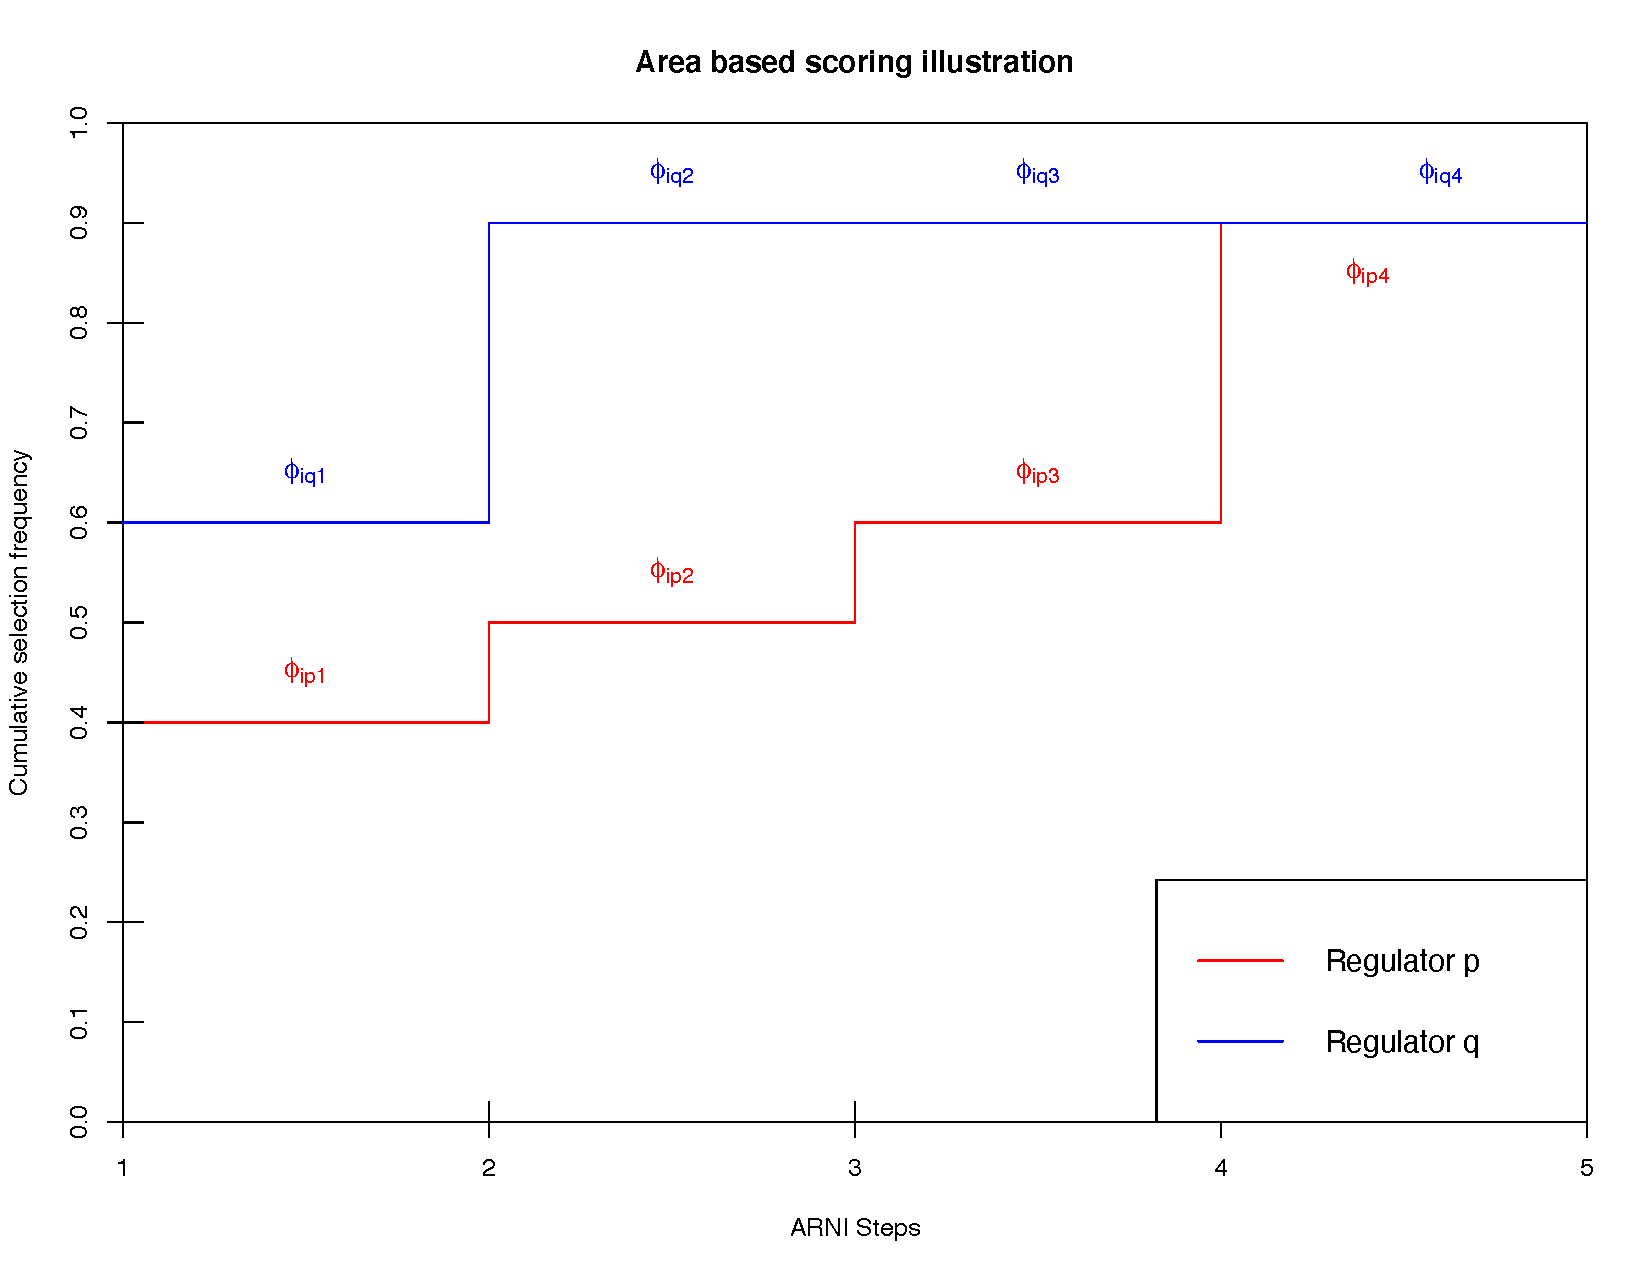
\includegraphics[width=0.8\textwidth]{area-scoring.pdf}
  \caption{基于面积的评分法示意图。针对目标基因 $i$ 的两个调控因子 $p$ 和 $q$,最后的得分 $S_{iq} > S_{ip}$。}
  \label{area-scoring}
\end{figure}


\subsubsection{计算复杂度}

基于改进数据驱动的基因调控网络构建方法 D3GRN 的计算复杂度主要取决于 ARNI,针对于每个目标基因复杂度为 $O(t^2*(tp)^3)$。
其中, $t$ 为转录因子的数目, $p$ 为基函数的数目 (即等式 (\ref{eq:xi_with_h})中的 $P_k$)。
$O((tp)^3)$ 是 BOLS 算法的 Moore-Penrose 伪逆计算时候的复杂度。
因此,针对 $n$ 个目标基因和 $b$ 轮抽样, D3GRN 的总体计算复杂度为 $O(t^5p^3nb)$。
由于 $t$ 通常比 $n$ 小得多,因此 D3GRN 的时间复杂度的上界是 $O(n^6p^3b)$。
具体运行的过程中,算法 \ref{alg:D3GRN} 中的``for"循环是完全可以并行的,可以在多核甚至分布式集群机器上同时进行。

\subsection{实验结果}

\subsubsection{数据集}

在实验中, 与上一章中使用的 DREAM3 数据集不同,
本文使用的是来自 DREAM4 和 DREAM5 挑战赛中的 6 个模拟数据集 \upcite{marbach2012wisdom}。
关于 DREAM 挑战赛的介绍, 在本文的第 \ref{subsubsec:loc-dataset} 章节中有详细介绍, 在此不再赘述。
本章实验所采用的 DREAM 数据集详情如表 \ref{datasets} 所示,其中 Network 表示数据集名称,
\#Genes 表示基因的数量, \#Regulators 表示调控因子的数量, \#Samples 表示样本的数量, 
\#Verified interactions 表示网络中的有向调控边数。
如果一个数据集用矩阵表示,那么行表示样本,列表示基因。
本文采用 DREAM4 挑战赛中的 5 个多因素数据集,
每个包含 100 个基因和 100 个样本。
这 5 个数据集中的样本是通过从原始数据中同时微扰动所有的基因, 借助于使用开源的 GeneNetWeaver 软件 \upcite{marbach2009generating} 辅助生成的。
因此,这 5 个数据集中的每个样本都代表了一个多因素扰动实验。
调控因子可以被看作是这些基因本身,因为挑战赛官方针对这 5 个网络没有指定哪些基因是调控因子。
%此外,我们从 DREAM5 数据集中选用了三个不同的和大小变化的网络。
本文还使用了一个 DREAM5 数据集 1,这也是一个由 GeneNetWeaver 模拟生成的网络。
这个模拟网络的拓扑结构是基于的已知的生物模型 GRNs 进行修正的。
与 DREAM4 中的网络不同的是,
DREAM5 数据集中的转录因子 (TFs) 集合是被挑战赛举办方显式提供的,它们是提供的所有基因的一个子集。

% while the other two expression datasets are real expression data collected 
% for E. coli (Network 3) and S. cerevisiae (Network 4). 
% It is observed that the performance of previous studies imply that Network 3 and Network 4 
% tend to be almost in a random manner.
% Accordingly, we only employ Network 1 dataset from DREAM5 datasets.
%as Network 3 and Network 4 in DREAM5 are more sparser than Network 1,
% Network 2 of DREAM5 is neglected in our experiments, 
% because there are no verified interactions provided for this dataset. 
% Network 3 and Network 4 in DREAM5 are more sparser than Network 1, 
% as they own more genes and regulators but less interactions.

\begin{table}[!htbp]
\centering
%\caption{Detail of the datasets}
\caption{实验数据集详情}

\label{datasets}
\resizebox{\columnwidth}{!}{%
\begin{tabular}{lccccc}
\toprule
Network           & \#Genes & \#Regulators & \#Samples & \#Verified interactions \\
\midrule
DREAM4  Network 1  & 100     & 100                & 100       & 176                      \\
DREAM4  Network 2  & 100     & 100                & 100       & 249                      \\
DREAM4  Network 3  & 100     & 100                & 100       & 195                      \\
DREAM4  Network 4  & 100     & 100                & 100       & 211                      \\
DREAM4  Network 5  & 100     & 100                & 100       & 193                      \\
%\hline
DREAM5 Network 1   & 1643    & 195                & 805       & 4012                   \\
%DREAM5 Network 3 (E. coli)       & 4511    & 334                & 805       & 2066                     \\
%DREAM5 Network 4 (S. cerevisiae) & 5950    & 333                & 536       & 3940                     \\
\bottomrule                   
\end{tabular}
}
\end{table}

\subsubsection{评价指标}

为了评估 GRN 推理算法的效果, 本文使用精确率-召回率曲线下的面积 (AUPR) 作为评价指标。
除了 AUPR 之外,接收者操作特征曲线下的面积 (AUROC) 也被广泛用于评估效果。
一般来说, AUROC 和 AUPR 值越高,说明 GRN 预测得越准确。
需要注意的是,在稀疏的生物网络中,不存在的边数目 (阴性边) 大大超过现有边的数量 (阳性边),
因而 AUPR 比 AUROC 更有参考价值 \upcite{saito2015precision} 。

本文首先通过比较金标准网络中的调节边和 D3GRN 的排序列表输出前 $q$ 条边,
计算出真阳性 (TP)、真阴性 (TN)、假阳性 (FP) 和假阴性 (FN) 边的数量。
随着 $q$ 不断增加, $q = 1,2,\ldots,N\times(N-1)$,其中 $N$ 为基因数,
通过绘制真阳性率 (The true positive rates, TPR) 与假阳性率 (The false positive rates, FPR) ,
便得到了接收者操作特征 (Receiver Operating Characteristic, ROC) 曲线; 
同样地,
%The ROC curve is constructed by plotting the true positive rates (TPR = TP/(TP + FN)) versus the false positive rates (FPR = FP/(FP + TN)) for increasing $q$ ($q = 1,2,\ldots,m^2$).
精确率-召回率 (Precision-Recall, PR) 曲线是通过绘制精确率 Precision 与召回率 Recall 而得到。
其中, TPR、FPR、Precision、Recall 的计算如第 \ref{sec:locpcacmi} 章的公式 \ref{eq:tpr}、\ref{eq:fpr}、\ref{eq:precision}、\ref{eq:recall} 所示。
本文再通过计算曲线下的面积便得到了 AUROC 和 AUPR。
%Similarly, the precision (TP/(TP + FP)) and recall (TP/(TP + FN)) curve is plotted for increasing $q$.

\subsubsection{实验结果分析}

等式 (\ref{eq:xi_with_h}) 中基函数的类型、阶数 $K$ 和基函数的数量 $P_k$ 在 ARNI 中的模型分解中起着至关重要的作用。
对于一大类动态系统,使用多项式非线性是充分的 \upcite{mangan2016inferring}。
作为参考,在本文基因调控网络的构建中,也采用了多项式基函数,
形式为 $h_{j,p}(x_j)=x_j^p$,基函数的数目表示为: 
\begin{equation}
P_k=\left\{\begin{matrix}
5,  k=1\\ 
0,  k>1
\end{matrix}\right. 
\end{equation}
这隐含表达了本文不考虑一个目标基因的 2 阶及以上的阶的交互作用。
事实上, bLARS \upcite{singh2016blars} 只考虑了一阶交互作用。
我们在本研究中也遵循这种简化的方式。
换句话说,其它基因对目标基因的调控是基于多项式非线性函数的混合。

D3GRN 中涉及到两个可变参数,
包括抽样次数 $b$ 和 ARNI 步数 $L$。
DREAM4 数据集中我们选用 DREAM4 网络 4 作为一个代表,
图 \ref{fig:performance_dr4_4} 展示了通过改变 ARNI 步数和抽样次数这两个参数后的 AUPR 值变化结果;
同样地, DREAM5 网络 1 的 ARNI 步数和抽样次数这两个参数对 AUPR 值的变化结果的影响如图 \ref{fig:performance_dr5} 所示。
一般来说,较大的抽样次数 $b$ 运行时间越长,但是它的性能会越趋于稳定和优异。
然而, D3GRN 的性能对抽样次数相当稳定,只要它大于某一阈值,通常是 200 次左右。
对于 ARNI 的步数 $L$,一个直觉是如果 $L$ 接近网络中先验的平均调控因子的数量,
那么结果将是最佳的,可以用 $\frac{\#\text{Verified interactions}}{\#\text{Genes}}$ 近似估计到。

\begin{figure}[!htbp]
  \centering
  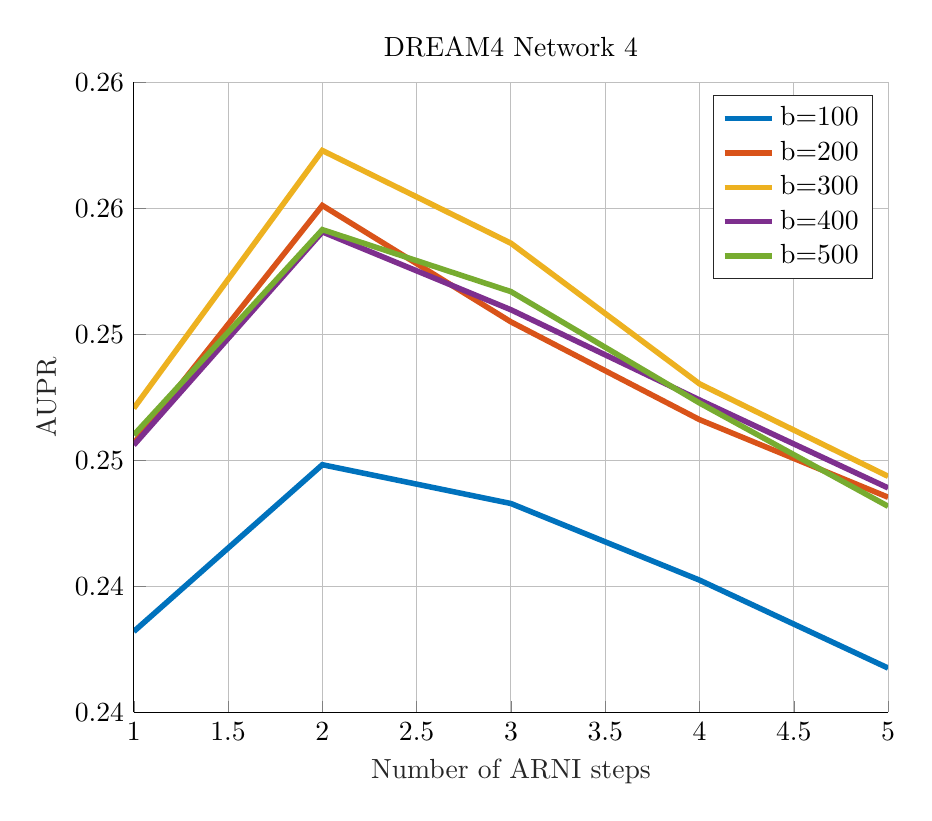
\begin{tikzpicture}

\definecolor{mycolor1}{rgb}{0.00000,0.44700,0.74100}%
\definecolor{mycolor2}{rgb}{0.85000,0.32500,0.09800}%
\definecolor{mycolor3}{rgb}{0.92900,0.69400,0.12500}%
\definecolor{mycolor4}{rgb}{0.49400,0.18400,0.55600}%
\definecolor{mycolor5}{rgb}{0.46600,0.67400,0.18800}%


\newlength{\fheight}
\newlength{\fwidth}
\setlength{\fheight}{8cm}
\setlength{\fwidth}{10cm}

\begin{axis}[%
width=0.958\fwidth,
height=\fheight,
at={(0\fwidth,0\fheight)},
scale only axis,
xmin=1,
xmax=5,
xlabel style={font=\color{white!15!black}},
xlabel={Number of ARNI steps},
ymin=0.235,
ymax=0.26,
ylabel style={font=\color{white!15!black}},
ylabel={AUPR},
axis background/.style={fill=white},
%title style={font=\bfseries},
title={DREAM4 Network 4},
axis x line*=bottom,
axis y line*=left,
xmajorgrids,
ymajorgrids,
legend style={legend cell align=left, align=left, draw=white!15!black}
]
\addplot [color=mycolor1, line width=2.0pt]
  table[row sep=crcr]{%
1	0.23821\\
2	0.24483\\
3	0.24329\\
4	0.24025\\
5	0.23676\\
};
\addlegendentry{b=100}

\addplot [color=mycolor2, line width=2.0pt]
  table[row sep=crcr]{%
1	0.24568\\
2	0.25512\\
3	0.2505\\
4	0.24662\\
5	0.24354\\
};
\addlegendentry{b=200}

\addplot [color=mycolor3, line width=2.0pt]
  table[row sep=crcr]{%
1	0.24707\\
2	0.2573\\
3	0.25362\\
4	0.24804\\
5	0.24437\\
};
\addlegendentry{b=300}

\addplot [color=mycolor4, line width=2.0pt]
  table[row sep=crcr]{%
1	0.24561\\
2	0.25407\\
3	0.25098\\
4	0.2474\\
5	0.24391\\
};
\addlegendentry{b=400}

\addplot [color=mycolor5, line width=2.0pt]
  table[row sep=crcr]{%
1	0.24601\\
2	0.25416\\
3	0.2517\\
4	0.24728\\
5	0.24318\\
};
\addlegendentry{b=500}

\end{axis}
\end{tikzpicture}%
  \caption{在 DREAM4 网络4 上不同的 ARNI 步骤数 $L$ 和抽样次数 $b$ 取得的 AUPR 值示意图。}
  \label{fig:performance_dr4_4}
\end{figure}

\begin{figure}[!htbp]
  \centering
  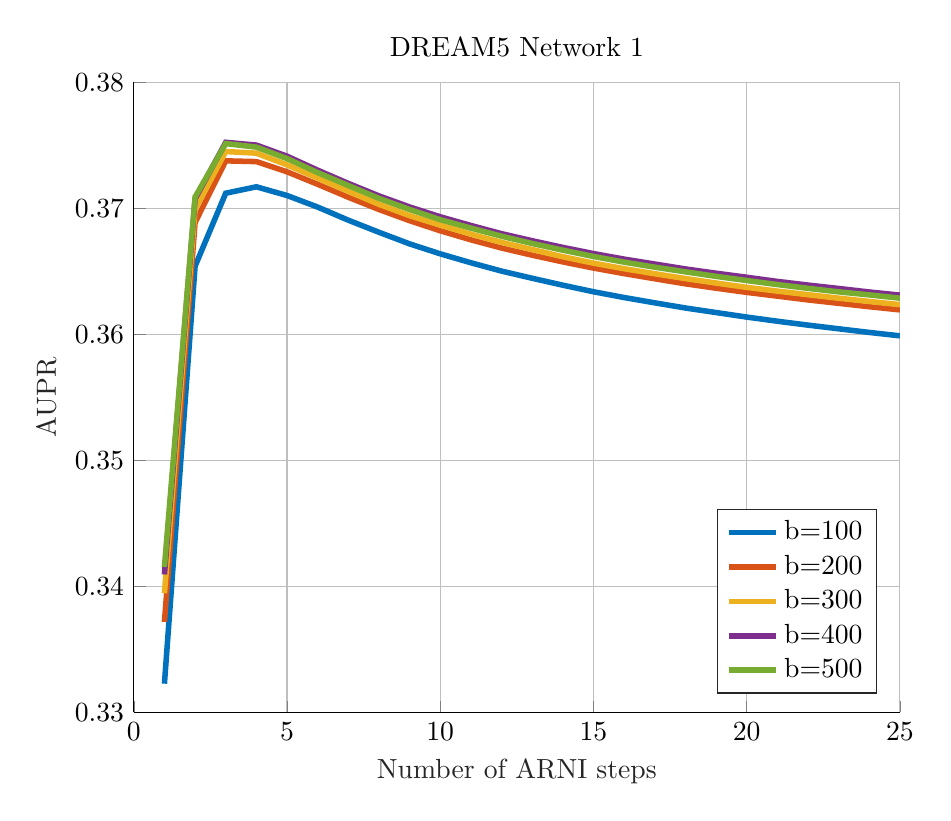
\begin{tikzpicture}

\definecolor{mycolor1}{rgb}{0.00000,0.44700,0.74100}%
\definecolor{mycolor2}{rgb}{0.85000,0.32500,0.09800}%
\definecolor{mycolor3}{rgb}{0.92900,0.69400,0.12500}%
\definecolor{mycolor4}{rgb}{0.49400,0.18400,0.55600}%
\definecolor{mycolor5}{rgb}{0.46600,0.67400,0.18800}%

\newlength{\fheight}
\newlength{\fwidth}
\setlength{\fheight}{8cm}
\setlength{\fwidth}{10cm}

\begin{axis}[%
width=0.973\fwidth,
height=\fheight,
at={(0\fwidth,0\fheight)},
scale only axis,
xmin=0,
xmax=25,
xlabel style={font=\color{white!15!black}},
xlabel={Number of ARNI steps},
ymin=0.33,
ymax=0.38,
ylabel style={font=\color{white!15!black}},
ylabel={AUPR},
axis background/.style={fill=white},
%title style={font=\bfseries},
title={DREAM5 Network 1},
axis x line*=bottom,
axis y line*=left,
xmajorgrids,
ymajorgrids,
legend style={at={(0.97,0.03)}, anchor=south east, legend cell align=left, align=left, draw=white!15!black}
]
\addplot [color=mycolor1, line width=2.0pt]
  table[row sep=crcr]{%
1	0.33228\\
2	0.36542\\
3	0.37121\\
4	0.37172\\
5	0.37103\\
6	0.37011\\
7	0.36907\\
8	0.36811\\
9	0.36719\\
10	0.3664\\
11	0.36569\\
12	0.36503\\
13	0.36446\\
14	0.36391\\
15	0.36339\\
16	0.36293\\
17	0.36251\\
18	0.3621\\
19	0.36174\\
20	0.36138\\
21	0.36105\\
22	0.36074\\
23	0.36045\\
24	0.36016\\
25	0.35989\\
};
\addlegendentry{b=100}

\addplot [color=mycolor2, line width=2.0pt]
  table[row sep=crcr]{%
1	0.33718\\
2	0.36889\\
3	0.37378\\
4	0.37372\\
5	0.37291\\
6	0.37192\\
7	0.37089\\
8	0.36992\\
9	0.36903\\
10	0.36823\\
11	0.36751\\
12	0.36686\\
13	0.36629\\
14	0.36576\\
15	0.36527\\
16	0.36483\\
17	0.36442\\
18	0.36402\\
19	0.36367\\
20	0.36334\\
21	0.36304\\
22	0.36274\\
23	0.36247\\
24	0.3622\\
25	0.36195\\
};
\addlegendentry{b=200}

\addplot [color=mycolor3, line width=2.0pt]
  table[row sep=crcr]{%
1	0.33946\\
2	0.36992\\
3	0.37452\\
4	0.37439\\
5	0.37346\\
6	0.37241\\
7	0.37136\\
8	0.37033\\
9	0.36943\\
10	0.36868\\
11	0.36796\\
12	0.36731\\
13	0.36674\\
14	0.36617\\
15	0.36566\\
16	0.36522\\
17	0.36482\\
18	0.36444\\
19	0.36408\\
20	0.36374\\
21	0.36344\\
22	0.36316\\
23	0.36288\\
24	0.36262\\
25	0.36237\\
};
\addlegendentry{b=300}

\addplot [color=mycolor4, line width=2.0pt]
  table[row sep=crcr]{%
1	0.34095\\
2	0.37077\\
3	0.37525\\
4	0.37503\\
5	0.37415\\
6	0.37304\\
7	0.37199\\
8	0.371\\
9	0.37012\\
10	0.36934\\
11	0.36865\\
12	0.368\\
13	0.36744\\
14	0.36691\\
15	0.36642\\
16	0.36598\\
17	0.36559\\
18	0.3652\\
19	0.36486\\
20	0.36454\\
21	0.36421\\
22	0.36392\\
23	0.36365\\
24	0.36337\\
25	0.36312\\
};
\addlegendentry{b=400}

\addplot [color=mycolor5, line width=2.0pt]
  table[row sep=crcr]{%
1	0.34154\\
2	0.37091\\
3	0.37515\\
4	0.37487\\
5	0.37396\\
6	0.37285\\
7	0.37182\\
8	0.3708\\
9	0.36992\\
10	0.36911\\
11	0.36844\\
12	0.3678\\
13	0.36722\\
14	0.36669\\
15	0.36619\\
16	0.36574\\
17	0.36534\\
18	0.36497\\
19	0.36461\\
20	0.36428\\
21	0.36396\\
22	0.36366\\
23	0.36338\\
24	0.36314\\
25	0.36288\\
};
\addlegendentry{b=500}

\end{axis}
\end{tikzpicture}

  \caption{在 DREAM5 网络1 上不同的 ARNI 步骤数 $L$ 和抽样次数 $b$ 取得的 AUPR 值示意图。}
  \label{fig:performance_dr5}
\end{figure}

本文分别在 DREAM4 和 DREAM5 网络进行了对比实验,来评测本文提出的方法 D3GRN。
NIMEFI 用 R 实现,而 GENIE3、TIGRESS 是用 MATLAB 实现。
这些方法的代码从对应论文提供的 URL 进行下载,在实验中各方法中的参数使用它们代码中推荐的默认值。
本文提出的方法 D3GRN 也是利用 MATLAB 实现的,使用的数据集及代码公开在 GitHub 仓库 \url{https://github.com/chenxofhit/D3GRN} 上。

表 \ref{tab:performance_dr4} 列出了 D3GRN 与其它 GRN 推理方法在五个 DREAM4 网络上比较的结果。
其中, D3GRN 的参数是在抽样次数 $b=200$, ARNI 步数 $L=2$ 下得到的。
如表所示,除了在 DREAM4网络 2 上, D3GRN 跟其它方法相比 AUPR 值最高。

表 \ref{tab:performance_dr5} 总结了 D3GRN 与其它 GRN 构建方法在 DREAM5 数据集上的比较结果。
D3GRN 的参数设置为抽样次数 $b=200$, ARNI步数 $L=5$。
D3GRN 在网络 1 上跟其它方法相比 AUPR 值最高。

% \begin{table*}[!htbp]
%   %\resizebox{\columnwidth}{!}{%
%   \centering
%   \begin{threeparttable}  
%   \caption{Performance comparisons of different GRN inference methods on the DREAM4 networks, challenge size 100 Multifactorial}  
%   \label{tab:performance_dr4} 
%     \begin{tabular}{ccccccccccc}  
%     \toprule  
%     \multirow{2}{*}{Method}&  
%     \multicolumn{2}{c}{Network 1}&\multicolumn{2}{c}{Network 2}&\multicolumn{2}{c}{Network 3}&\multicolumn{2}{c}{Network 4}&\multicolumn{2}{c}{Network 5}\\
%     \cmidrule(lr){2-3} \cmidrule(lr){4-5}  \cmidrule(lr){6-7}  \cmidrule(lr){8-9} \cmidrule(lr){10-11}
%     &AUPR&AUROC &AUPR&AUROC &AUPR&AUROC &AUPR&AUROC &AUPR&AUROC\\
%     \midrule  
%     GENIE3  &0.161 &0.750        &0.154&0.734         &0.234&0.776          &0.211&0.800         &0.200&0.795    \\
%     TIGRESS &0.158 &0.747        &0.161&0.703         &0.233&0.761          &0.225&0.774         &0.233&0.754     \\
%     NIMEFI  &0.157 &\textbf{0.758}        &0.157&0.731         &0.248&0.776          &0.225&0.806         &0.241&\textbf{0.801}     \\
%     PLSNET  &0.118 &0.713        &\textbf{0.290}&\textbf{0.828}         &0.202&\textbf{0.794}          &0.228&\textbf{0.819}         &0.206&0.786     \\
%     \textbf{D3GRN}    &\textbf{0.175} &0.704        &0.136&0.683         &\textbf{0.253}&0.734          &\textbf{0.255}&0.778         &\textbf{0.247}&0.732     \\
%     \bottomrule  
%     \end{tabular}  
%    \end{threeparttable}
%  %   }
% \end{table*} 

\begin{table}[!htbp]
  %\resizebox{\width}{0.8}{%
  %\resizebox{\textwidth}{20mm}{
  \centering
  \begin{threeparttable}  
%  \caption{Performance comparisons of different GRN inference methods on the DREAM4 networks in terms of AUPR}
  \caption{不同 GRN 构建方法在 DREAM4 网络上的 AUPR 结果}

  \label{tab:performance_dr4} 
    \begin{tabular}{cccccc}  
    \toprule  
    Method
     & Network 1&  Network 2&  Network 3&  Network 4 & Network 5\\
    \midrule  
    GENIE3  &0.161   &0.154           &0.234      &0.211          &0.200                 \\
    TIGRESS &0.158   &\textbf{0.161}           &0.233      &0.225          &0.233                \\
    NIMEFI  &0.157   &0.157           &0.248      &0.225          &0.241                \\
    % PLSNET  &0.118   &\textbf{0.290}  &0.202      &0.228          &0.206                \\
    \textbf{D3GRN}   &\textbf{0.175}  &0.136      &\textbf{0.253} &\textbf{0.255}       &\textbf{0.247}  \\
    \bottomrule  
    \end{tabular}  
   \end{threeparttable}
  %}
\end{table} 

\begin{table}[!htbp]
% \scalebox{0.6}{
% \begin{minipage}{2\linewidth}  
  \centering  
  %\fontsize{6.5}{8}\selectfont  
   % \resizebox{\columnwidth}{!}{%
  \begin{threeparttable}  
%  \caption{Performance comparisons of different GRN inference methods on the DREAM5 Network 1 in terms of AUPR}  
  \caption{不同 GRN 构建方法在 DREAM5 网络 1 上的 AUPR 结果}

  \label{tab:performance_dr5} 
    \begin{tabular}{ccccccc}  
    \toprule  
    Network&GENIE3 &TIGRESS &NIMEFI  &\textbf{D3GRN}\\
    \midrule  
    Network 1&0.291 &0.302 &0.298 &\textbf{0.373}\\
    \bottomrule  
    \end{tabular}  
    \end{threeparttable}
    %}
\end{table} 


\subsection{小结}

在 GRN 构建中, 基因与基因的调控作用所形成的网络存在稀疏的结构这一假设是合理的,
特别是在``小 $n$ 大 $p$"的情况下, 即可用的测序基因表达样本数量少,基因数量多。
在 GRN 中,稀疏性假设意味着每个基因只有少量的调控因子,这个假设也很合理,
本文提出的 D3GRN 方法也遵循同样的假设,并且我们还认为,其它基因对目标基因的调控是基多项式非线性函数的混合作用。
本文在 DREAM4 和 DREAM5 数据集上评估了我们的方法。
本文方法的实验结果也验证了这一假设,至于这个假设的理论和生物实验分析需要后续的工作来支持。

另一个重要问题是关于 D3GRN 的计算复杂度。
客观地讲, ARNI 适合于构建节点级的小型物理动态网络。
ARNI 采用的 BOLS 算法的 Moore-Penrose 伪逆运算,对于大型生物网络来说是很耗时的。
D3GRN 中采用的抽样策略使其在处理大规模 GRNs 推理时,
针对单个的子网络而言由于对样本抽样后的数据样本规模减小,
在一定程度上提升了单次运行的性能。
关于 ARNI 的改进空间, D3GRN 中抽样策略中的``for" 循环是完全可以并行的,
可以在多核甚至集群中的分布式机器上同时进行。
这也值得其它方法尝试,比如用 BOMP \upcite{majumdar2009fast}来替代 BOLS 算法,这是留给未来的工作。
目前最先进的算法性能的差异性表明,
没有一种算法在所有数据集上都表现得同样出色。
然而,所有这些算法都可以应用于为元算法 (meta algorithm) 提供输入,
利用``群体智慧" (Wisdom of crowds) 来创建一个共识和可靠的社区网络 \upcite{Marbach2012a,zheng2008gene}。
另外,从小网络到大网络,所有算法的性能都在下降,这或许反应了不同规模的底层调控网络的复杂性在增加。
本文提出的方法推进了当前的技术水平, 但要把这个难题完全攻克下来, 还需要有很长的路要走。

从基因表达数据中构建 GRNs 是一项重要的任务,
可以促进我们对系统生物学中疾病和癌症等基本机制的理解。
最近数据驱动的动态网络构建方法为本文构建 GRNs 提供了新的视角。
在本研究中,本文提出了一种数据驱动的动态网络构建方法来构建基因调控网络,
该方法将每个目标基因的调控关系转化为函数分解问题,并利用揭示网络相互作用的算法 ARNI 来构造局部 GRN。
然而,传统的数据驱动的动态网络恢复方法,如 SINDy 和 ARNI 不具备构建全局网络的能力。
本文采用抽样和基于面积的评分策略克服了这一缺陷,从而构建出最终的全局 GRN。
在 DREAM4 和 DREAM5 基准数据集上的实验结果表明, D3GRN 在 AUPR 方面的表现具有竞争力。


\newpage
\section{单细胞 RNA-seq 数据下的细胞类型识别方法}
\label{sec:rafclust}

\subsection{引言}

基因调控与细胞类型密切相关 \cite{Hocker2020.09.11.291724,kang2020learning},
细胞聚类也是单细胞 RNA-seq 数据分析的热门和重要的问题, 
因此构建基因调控网络的一个不可或缺的前置任务是在单细胞数据集上对细胞的异质性进行聚类分析。
由于单细胞 RNA-seq 对于每个细胞测得的读数有限,细胞在测序过程中也会发生粘连,
因此导致每个细胞很多的基因表达量为 0,
这种现象被称之为单细胞的 dropout \cite{vallejos2017normalizing}。
同时,单细胞 RNA-seq 测序中将基因作为特征,常见的人和老鼠两种物种都有 20000 多个基因,
这种高维特征也给单细胞 RNA-seq 数据上的聚类带来挑战 \cite{stegle2015computational}。

在单细胞数据上的细胞类型识别上,除了聚类之外,还有一个十分具有挑战性的问题,即是如何从超大规模的 scRNA-seq 数据中识别稀有细胞。
稀有细胞代表了生物体内的次要细胞类型,当测序细胞的数量在数百个规模时,一个孤立的离群点 (singleton) 也很值得关注。
然而,随着吞吐能力的提高,研究重点转换到次要细胞类型的发现,再也不仅仅是单纯的单个细胞。
稀有细胞类型包括循环肿瘤细胞、癌症干细胞、循环内皮细胞、内皮祖细胞、抗原特异性 T 细胞、不变性自然杀伤性 T 细胞等。
尽管丰度较低,但稀有细胞群在决定癌症的发病机制、介导免疫反应、癌症和其它疾病的血管生成等方面起着核心作用。
抗原特异性 T 细胞对免疫学记忆的形成至关重要 \cite{slansky2003antigen,altman1996phenotypic,manzo2015antigen}。
内皮祖细胞,来源于骨髓,已被证明是肿瘤血管生成的可靠生物标志物 \cite{kuo2012dynamics,cima2016tumor}。
干细胞可以替代受损细胞,并用于治疗帕金森氏症、糖尿病、心脏病等疾病 \cite{jang2005stem}。
循环肿瘤细胞提供了前所未有的视角,为临床管理提供了实时的线索和根据 \cite{krebs2010circulating}。
现有的寻找稀有细胞的算法大部分依赖单细胞聚类方法,
在处理超大规模 scRNA-seq 数据时候非常耗时或者耗费内存。

本章中,我们提出了一种高效准确的单细胞聚类方法 RafClust。
针对当前单细胞 RNA-seq 数据集上细胞聚类不够准确鲁棒的问题,
我们使用多种相关性度量方法来刻画细胞的特征, 
然后使用随机森林回归模型进一步学习细胞与细胞之间的相似性矩阵,
基于相似性矩阵后采用层次聚类来决定细胞的最终类别。
实验结果表明,在十个单细胞数据集上, RafClust 在 ARI 上表现优于其它六种方法。

针对超大规模的 scRNA-seq 数据, 本文在 RafClust 方法的基础上进一步提出了一种高效准确的单细胞稀有细胞识别方法 DoRC (Discovery of Rare Cells)。
DoRC 产生的稀有度分数可以帮助生物学家们着重于下游分析,只对超大规模内的部分表达细胞 scRNA-seq 数据进行分析。
借助于单细胞聚类方法 RafClust,DoRC 可以进一步划分出准确的稀有细胞类型。
在超大规模的 scRNA-seq 数据 ${\sim}68$k 人血细胞的单细胞表达谱上,
 DoRC 在划分人类血液树突状细胞亚型方面有突出的效果, 执行效率高。
另外, DoRC 可以识别仿真数据集里面的稀有细胞,并且对细胞类型特征也很敏感。

\subsection{相关工作}

基于单细胞 RNA-seq 的细胞异质性研究主要是根据每个细胞的基因表达量来计算细胞之间的相似性,
结合聚类方法来确定细胞的类别。国内外研究者针对单细胞 RNA-seq 数据上的异质性研究已取得不少成果。
一类方法是最传统的聚类方法,比如使用 t-SNE 对数据进行降维然后使用 K-means 对数据进行聚类。
显然这种方法对噪声十分敏感。
Gr{\"u}n 等人 \cite{grun2016novo} 提出的 RaceID2 
使用 K-medoids 方法聚类,依据类内散布饱和临界值为依据确定分类个数。
另一类方法的研究思路是通过对原始数据进行插值处理 (imputation),减轻 scRNA-seq 数据中的 dropout 的影响。
典型的方法比如 Lin 等人提出的 CIDR 方法 \cite{lin2017cidr}。
CIDR 对 dropout 与基因表达值的关系进行了建模, 通过隐式插值处理后获取细胞与细胞之间的非相似性矩阵,
然后使用层次聚类获得最终的结果。
还有一类最流行的方法的研究思路是通过提高细胞与细胞之间的相似性计算的准确度和鲁棒性。
Kiselev 等人 \cite{kiselev2017sc3} 提出了一种共识聚类方法 SC3。
SC3 基于计算细胞与细胞间的 Pearson、Spearman 和欧氏距离三种不同相似性和主成分分析、拉普拉斯转换分别获得多个聚类结果,
然后通过计算这些聚类结果中两个细胞被聚为一类的数目来构建共识矩阵,
最后利用层次聚类获得最终的结果。
Wang 等人 \cite{wang2018simlr} 提出了无监督的 SIMLR 聚类方法。
SIMLR 构建不同粒度的高斯核矩阵来学习细胞与细胞之间的距离 (相似性) 矩阵,
并使用已有的比如 K-means 来获得每个细胞的类型。
Yang 等人 \cite{yang2018safe} 提出了聚合聚类方法 SAFE。
SAFE 选用了 SC3、CIDR、Seurat 和 t-SNE + K-means 四种聚类方法,
基于超图划分算法聚合四种聚类方法的结果。
Pouyan 等人 \cite{pouyan2018random} 提出了一种基于随机森林的计算细胞相似性的方法 RAFSIL。
RAFSIL 首先对基因过滤和聚类,接着对每个基因模块使用主成分降维,合并后作为随机森林的输入,
根据两个细胞落入同一颗决策树叶子上的数目计算细胞的相似性,然后使用层次聚类或者 K-means 获取每个细胞的类型。
相比于 SIMLR, RAFSIL 在聚类效果上有一定的提高,
但由于对基因聚类以及使用多颗决策树回归时,细胞数目一旦增加,计算效率显著降低。

scRNA-seq 技术的另外一个非常迫切和具有挑战性的应用,是从组织中的一堆细胞中捕获稀有细胞。
最近基于液滴 (Drop) 的单细胞转录组测序技术的发展,使得数以万计的单细胞的并行测序成为可能。
单个细胞的测序成本显著降低的情况下,稀有细胞的鉴别也变为可行。
迄今为止,已经有许多研究发表了可公开使用的转录组,细胞数量范围在 ${\sim} 20$k 和 ${\sim} 70$k 之间。
大规模的转录组样本通过削弱由于扩增阶段的失败所带来的影响,可以更好地捕捉到组织中的微小细胞亚群。
事实上,稀有细胞检测已经成为目前下游分析流程中的不可缺少的一环。
到目前为止,聚焦于研究怎样去检测稀有细胞转录组的算法还很少,
其中代表性的方法有 RaceID \cite{grun2015single}, GiniClust \cite{jiang2016giniclust} 和 FiRE \cite{jindal2018discovery}。
RaceID 涉及到计算成本十分高昂的参数模型,并用于检测离群的表达谱值。
它使用了 \textit{k}-means 聚类这种典型的基于距离的方法和间隙统计计算,
来作为识别大量细胞类型的中间步骤。
 GiniClust 使用了双管齐下的方法,
它首先使用 Gini 系数选择信息量大的基因,
然后它使用基于密度的空间聚类应用与噪声 (DBSCAN) \cite{ester1996density} 来发现离群细胞。
值得注意的是, RaceID 和 GiniClust 都使用聚类步骤来区分主要和次要细胞类型。
对于超大的 scRNA-seq 数据来说,速度非常慢,而且内存使用效率低。
相比之下, FiRE 为研究中的每一个细胞表达谱计算出一个稀有度分数。
它使用 Sketching 技术 \cite{wang2007sizing}来估计每个细胞的密度,
对于大规模细胞的低维编码来说, FiRE 运行速度非常快。

\subsection{基于随机森林相似性学习的单细胞聚类方法 RafClust}
\label{sec:method}

RafClust 方法对 scRNA-seq 数据进行细胞聚类,包括几个子步骤,如图 \ref{fig:rafclust} 所示, 这些步骤的细节将在下文中详述。
\begin{figure}[!htbp]
    \centering
    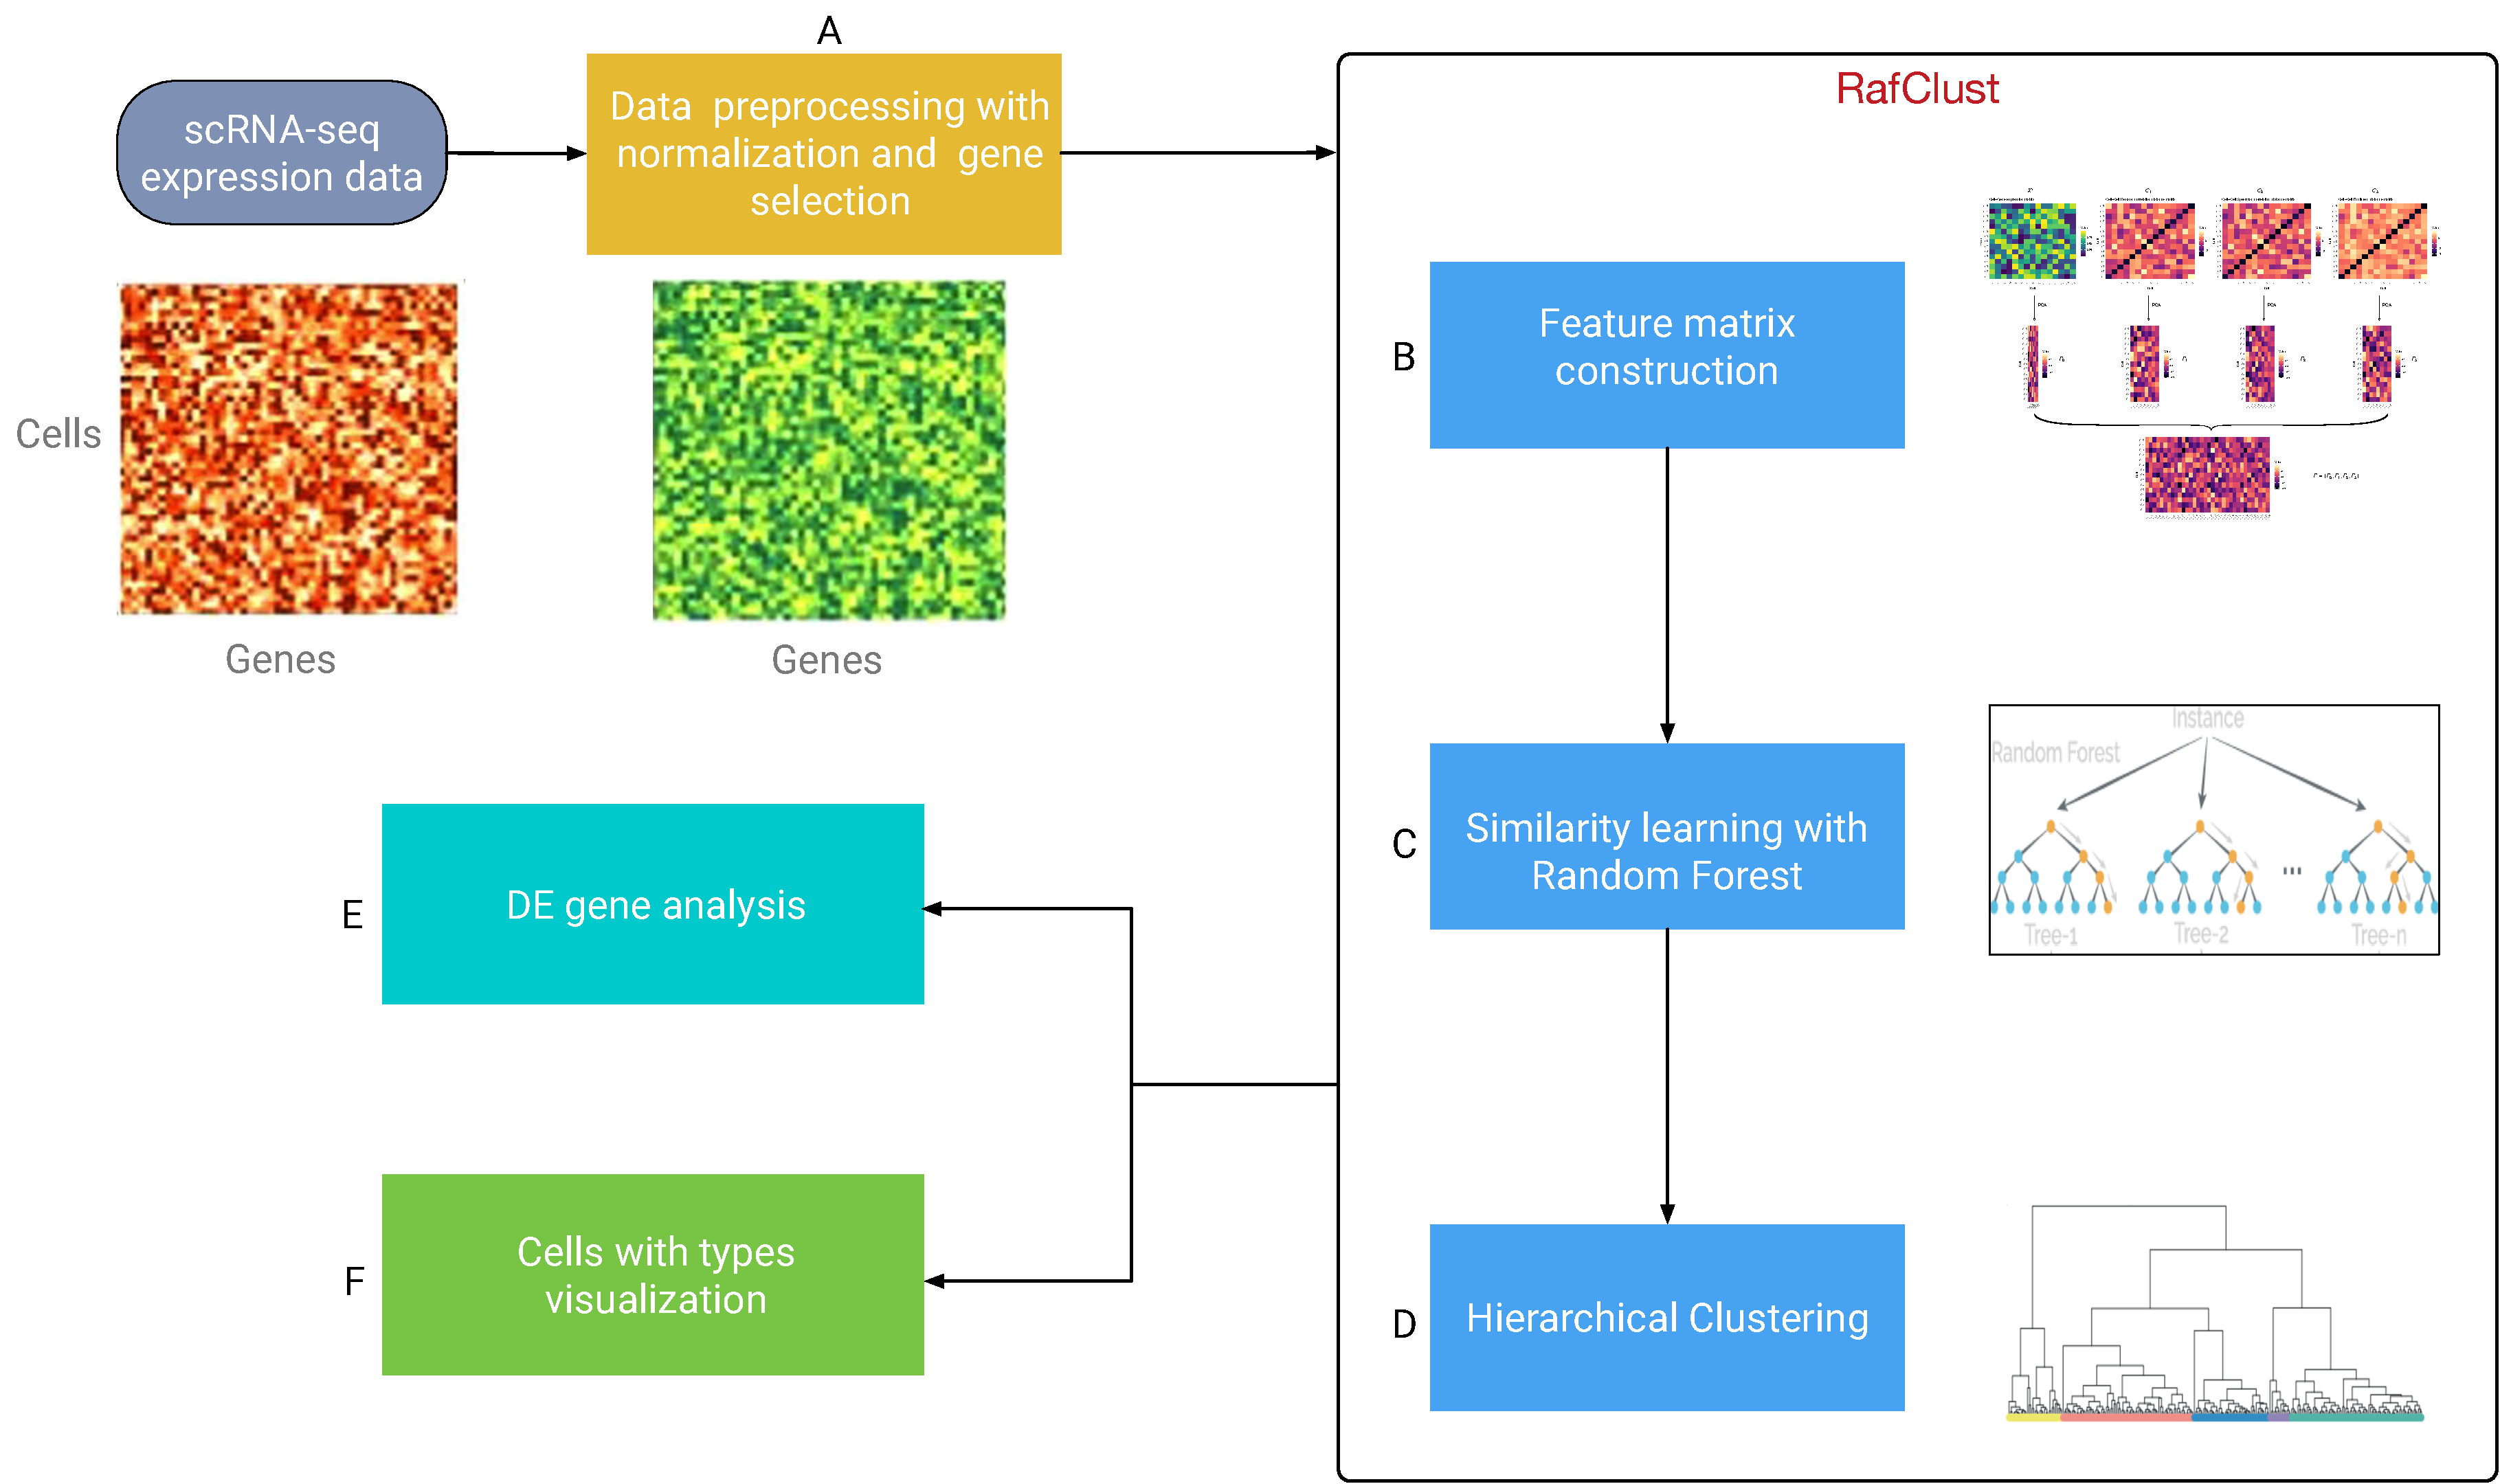
\includegraphics[width=0.95\textwidth]{flowchart-rafclust.pdf}
    \caption{RafClust 流程图。
    本图中的每个注释图代表了相应过程的输入或输出可视化。输入的是 scRNA-seq 表达数据二维矩阵,其中行代表细胞,列代表基因。
    (A) 用输入的表达数据进行数据预处理,输出的是一个归一化和列的维度缩减的矩阵。
    (B-D) RafClust 的核心程序。
    (B) 利用表达数据构造特征矩阵。
    (C) 利用随机森林算法来学习细胞与细胞的相似性矩阵。
    (D) 利用层次聚类来对细胞进行聚类。
    (E) 对不同类型的细胞进行不同的差异基因分析,从而得到细胞类型的特异基因。
    (F) 细胞表达数据与其类型可视化,在基于 t-SNE 的二维图中不同的颜色代表不同的细胞类型。
    }
    \label{fig:rafclust}
\end{figure}

\subsubsection{数据规范化和基因选择}
\label{subsec:datapreprocessing} 

我们假设归一化的 $n$ 个细胞的基因表达数据 (观测值), 每个细胞含有 $p$ 个基因(特征),
组成一个 $n \times p$ 的表达式矩阵 $X=\left(x_{1}, x_{2}, \ldots, x_{n} \right)^ T$。
其中 $x_{i}$ 表示 $p$ 基因在细胞 $i$ 中的表达值。
$x_{i}=\left(x_{i1}, x_{i2},\ldots, x_{ip} \right)$。
矩阵 $X$ 在加上 1 的伪数 (pseudo-count) 后进行对数变换,即 $X^{\prime} = log_2 (X + 1)$。
然后,如果基因在细胞总数中的表达低于一个预定频率 $\beta$,则该基因会被过滤掉。
默认情况下, $\beta$ 设置为 0.06 \cite{kiselev2017sc3}。 
基因过滤的动机是,除了保守的基因外,其它一些很普通的甚至是低表达的基因往往对细胞的聚类没有贡献。

\subsubsection{细胞类型识别}
\label{subsec:rafclust} 
为了从稀有细胞集合中确认不同的细胞类型,我们提出了一种无监督的基于随机森林的相似性学习算法,命名为 RafClust。
类似于其它的许多方法 \cite{kiselev2017sc3,pouyan2018random,mohammadi2018geometric,sinha2018dropclust,Srinivasan511626,Li530378,zheng2019sinnlrr},
RafClust 也是两个步骤的方法,
第一个步骤是我们使用随机森林进行相似度学习 (相似性学习步骤, similarity learning),
第二个步骤中我们使用层次聚类 (聚类步骤, clustering)。
在相似度学习步骤中,一个非常关键的预处理程序是特征矩阵的构建。
稀有细胞 (rare cells) 与丰富细胞 (abundant cells) 不同,我们将使用细胞和细胞的尽量多的不同类型的相似性,来充分刻画稀有细胞的本性特征。
因此,在基于基因过滤后的表达矩阵 $X^{\prime}$ 上,
我们利用欧几里德 (Euclidean)、皮尔逊 (Pearson) 和斯皮尔曼 (Spearman) 指标分别计算出三种不同的细胞-细胞距离矩阵 $\{C_1, C_2, C_3\}$。
然后将主成分分析 PCA 应用于每个距离矩阵,也应用于 $X^{\prime}$ 上,来减少数据维度的同时也去除其本能噪声。
每个矩阵中信息量最大的成分由``elbow 法" \cite{thorndike1953belongs} 保留,
这样就共计产生了 $\left\{ {F}_{i} \in \mathbb {R} ^ {n \times m_{i}} \right\}_{i = 0}^{3}$ 四个矩阵。
最终的特征矩阵 $F$ 由这些矩阵按行拼接组成, 行代表细胞, 列代表手工特征 (handcrafted features)\footnote{区分于现在比较流行的深度学习里的 auto-learned features}。
\begin{equation}
\label{lab:f}
{F} = ({F}_{0}, {F}_{1}, {F}_{2}, {F}_{3})
\end{equation}

$F$ 中的列数 (维度) (即特征总数 $\tilde {p} = \sum_{i = 1}^{k} m_{i}$) 与数据有关。
和细胞 $j$ 现在用特征向量 $f_{i} \in \mathbb {R} ^ {\tilde{p}}$ 表示。
显然,$F$ 既反应了细胞的自身表达值,也包含了细胞与其它细胞的相似性关系特征。
接着,我们利用特征矩阵 $F$ 来进行基于随机森林 (RF) 的相似性学习。
图 \ref{fig:rafsim} 是一个示例,在大小为 $15 \times 15$ 基因表达矩阵的数据集上来说明整个特征矩阵的构建步骤。

% \begin{figure}[!htbp]
%   \begin{adjustbox}{addcode={
%     \begin{minipage}{\width}}{
%         \caption{一个有 15 个细胞和每个细胞 15 个基因的示例数据集中手动制作的特征矩阵构造。
%         最终的特征矩阵 $F$ 在这个示例中是 $15\times34$ 维度大小的。}
%         \label{fig:rafsim}
%     \end{minipage}},rotate=90,center}
%     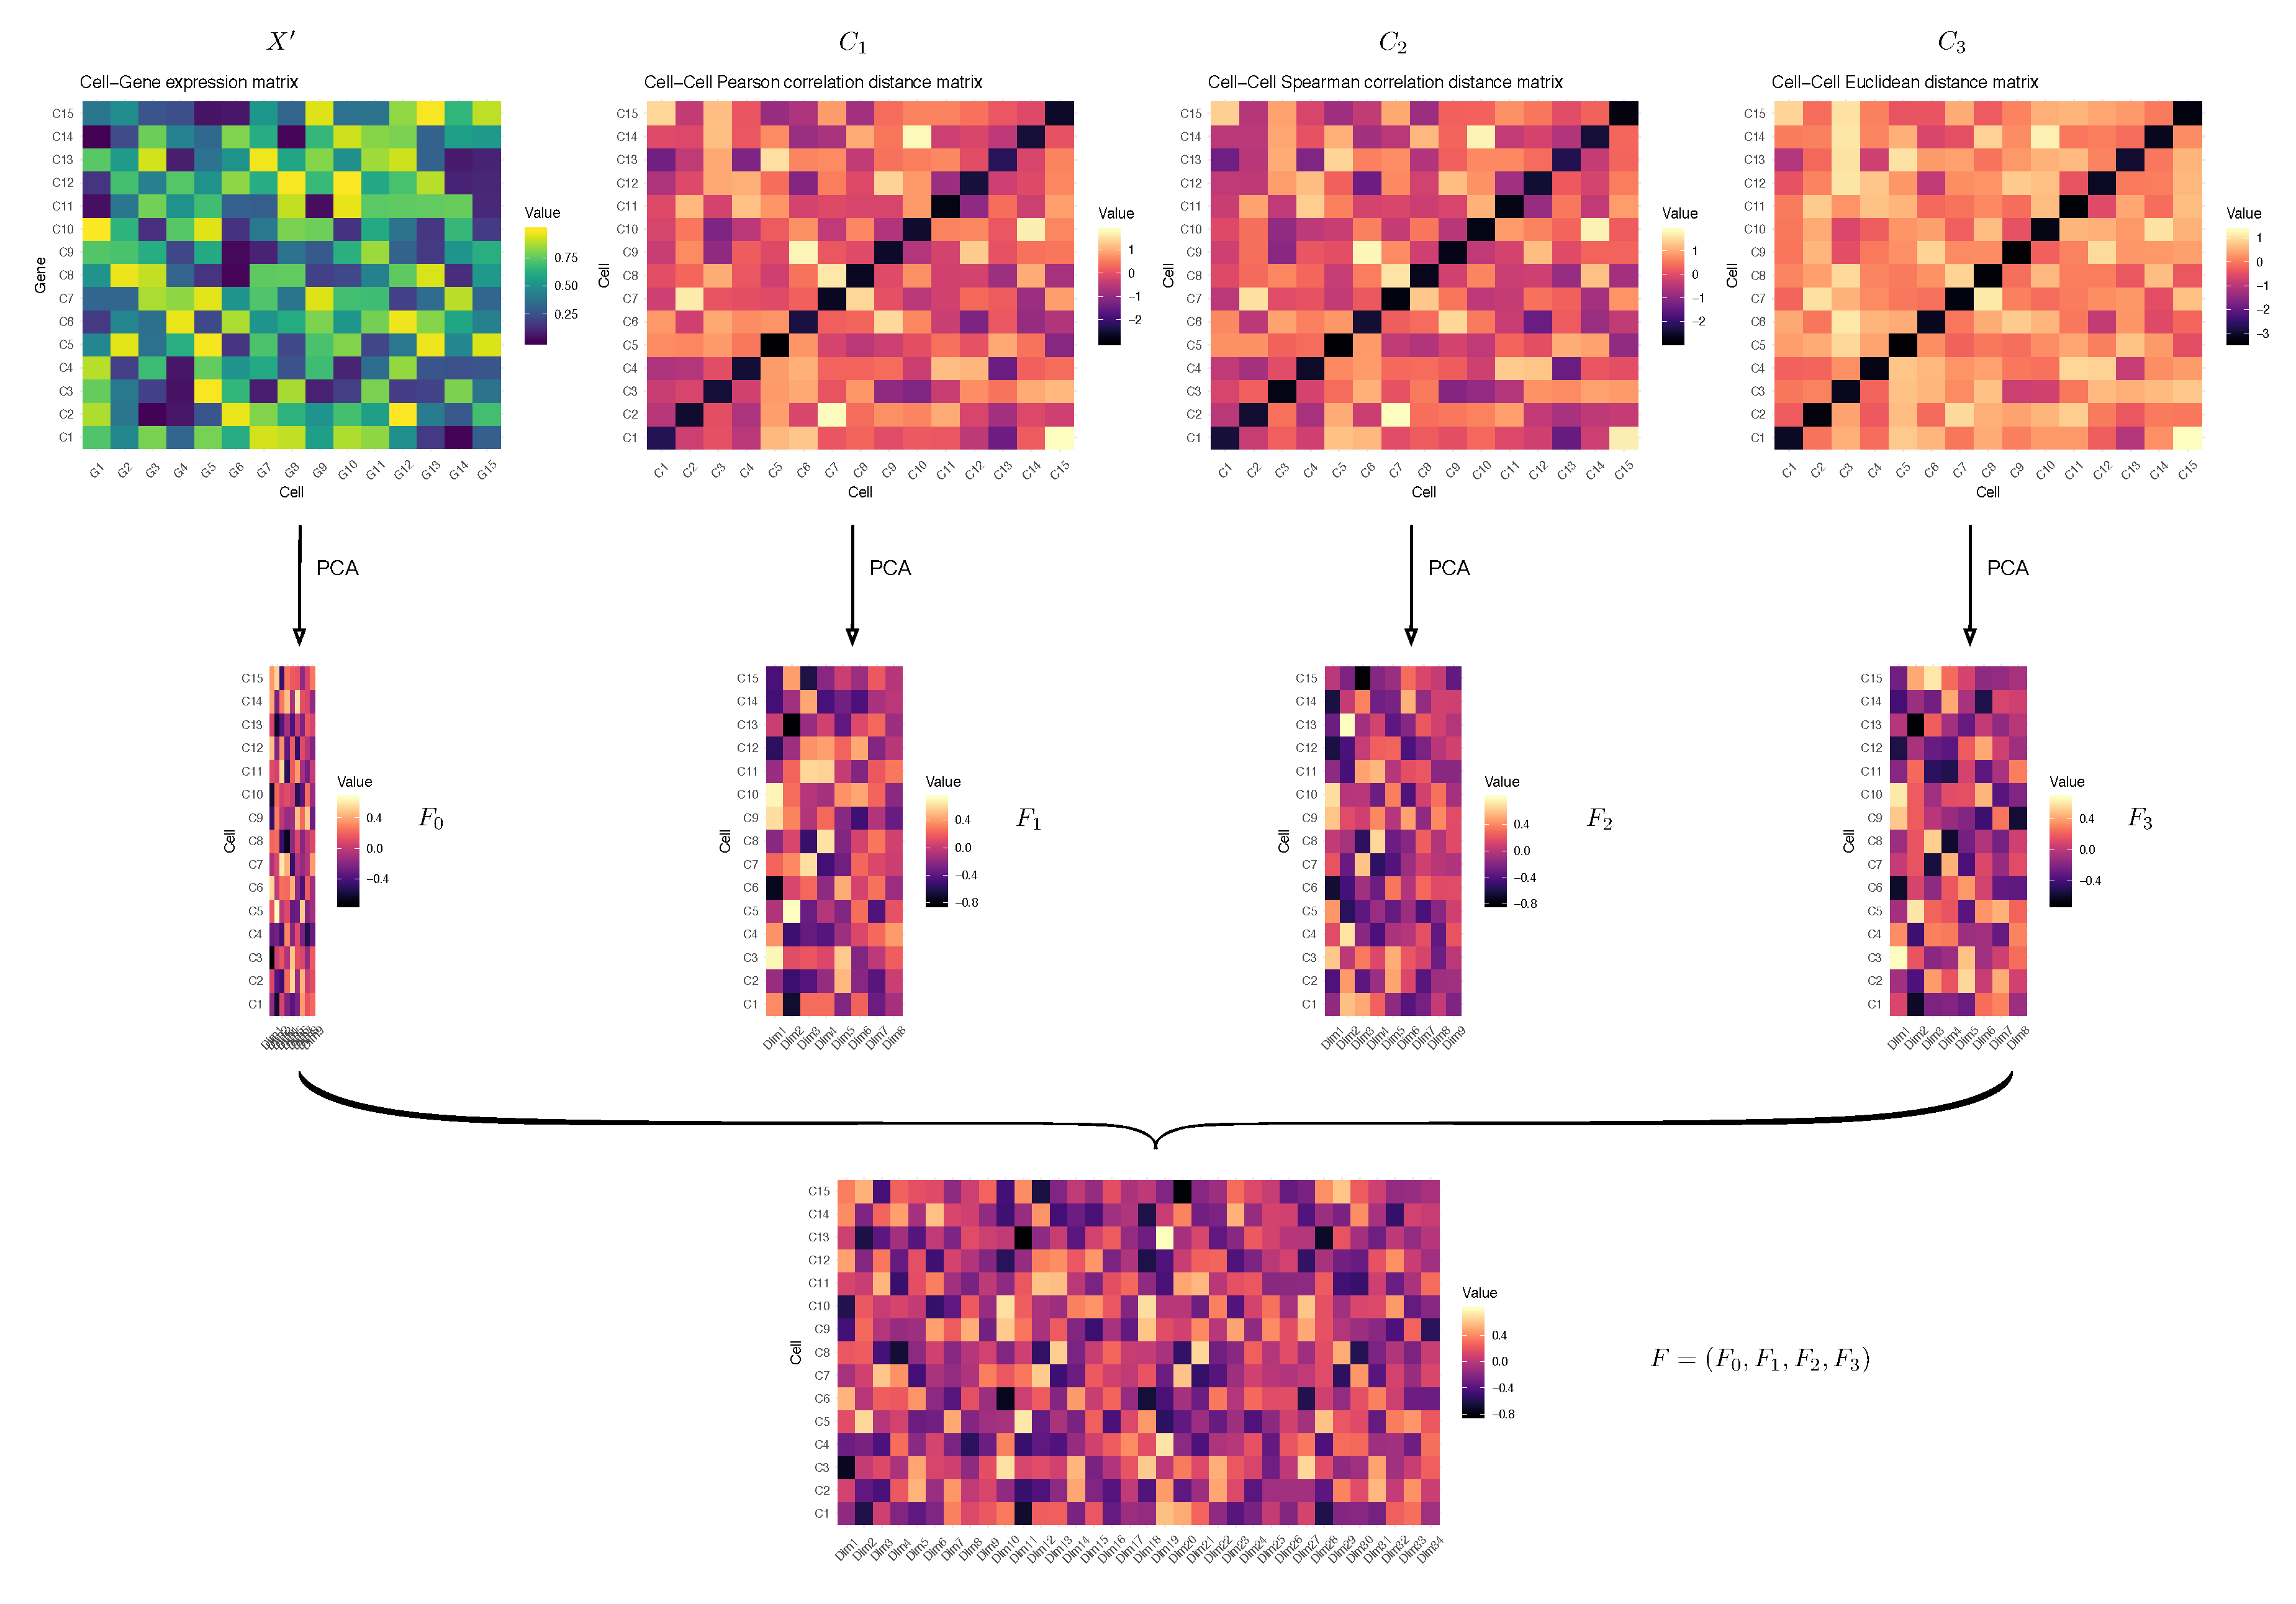
\includegraphics[scale=.42]{rafsim.pdf}%
%   \end{adjustbox}
% \end{figure}
\begin{figure}[!htbp]
    \centering
    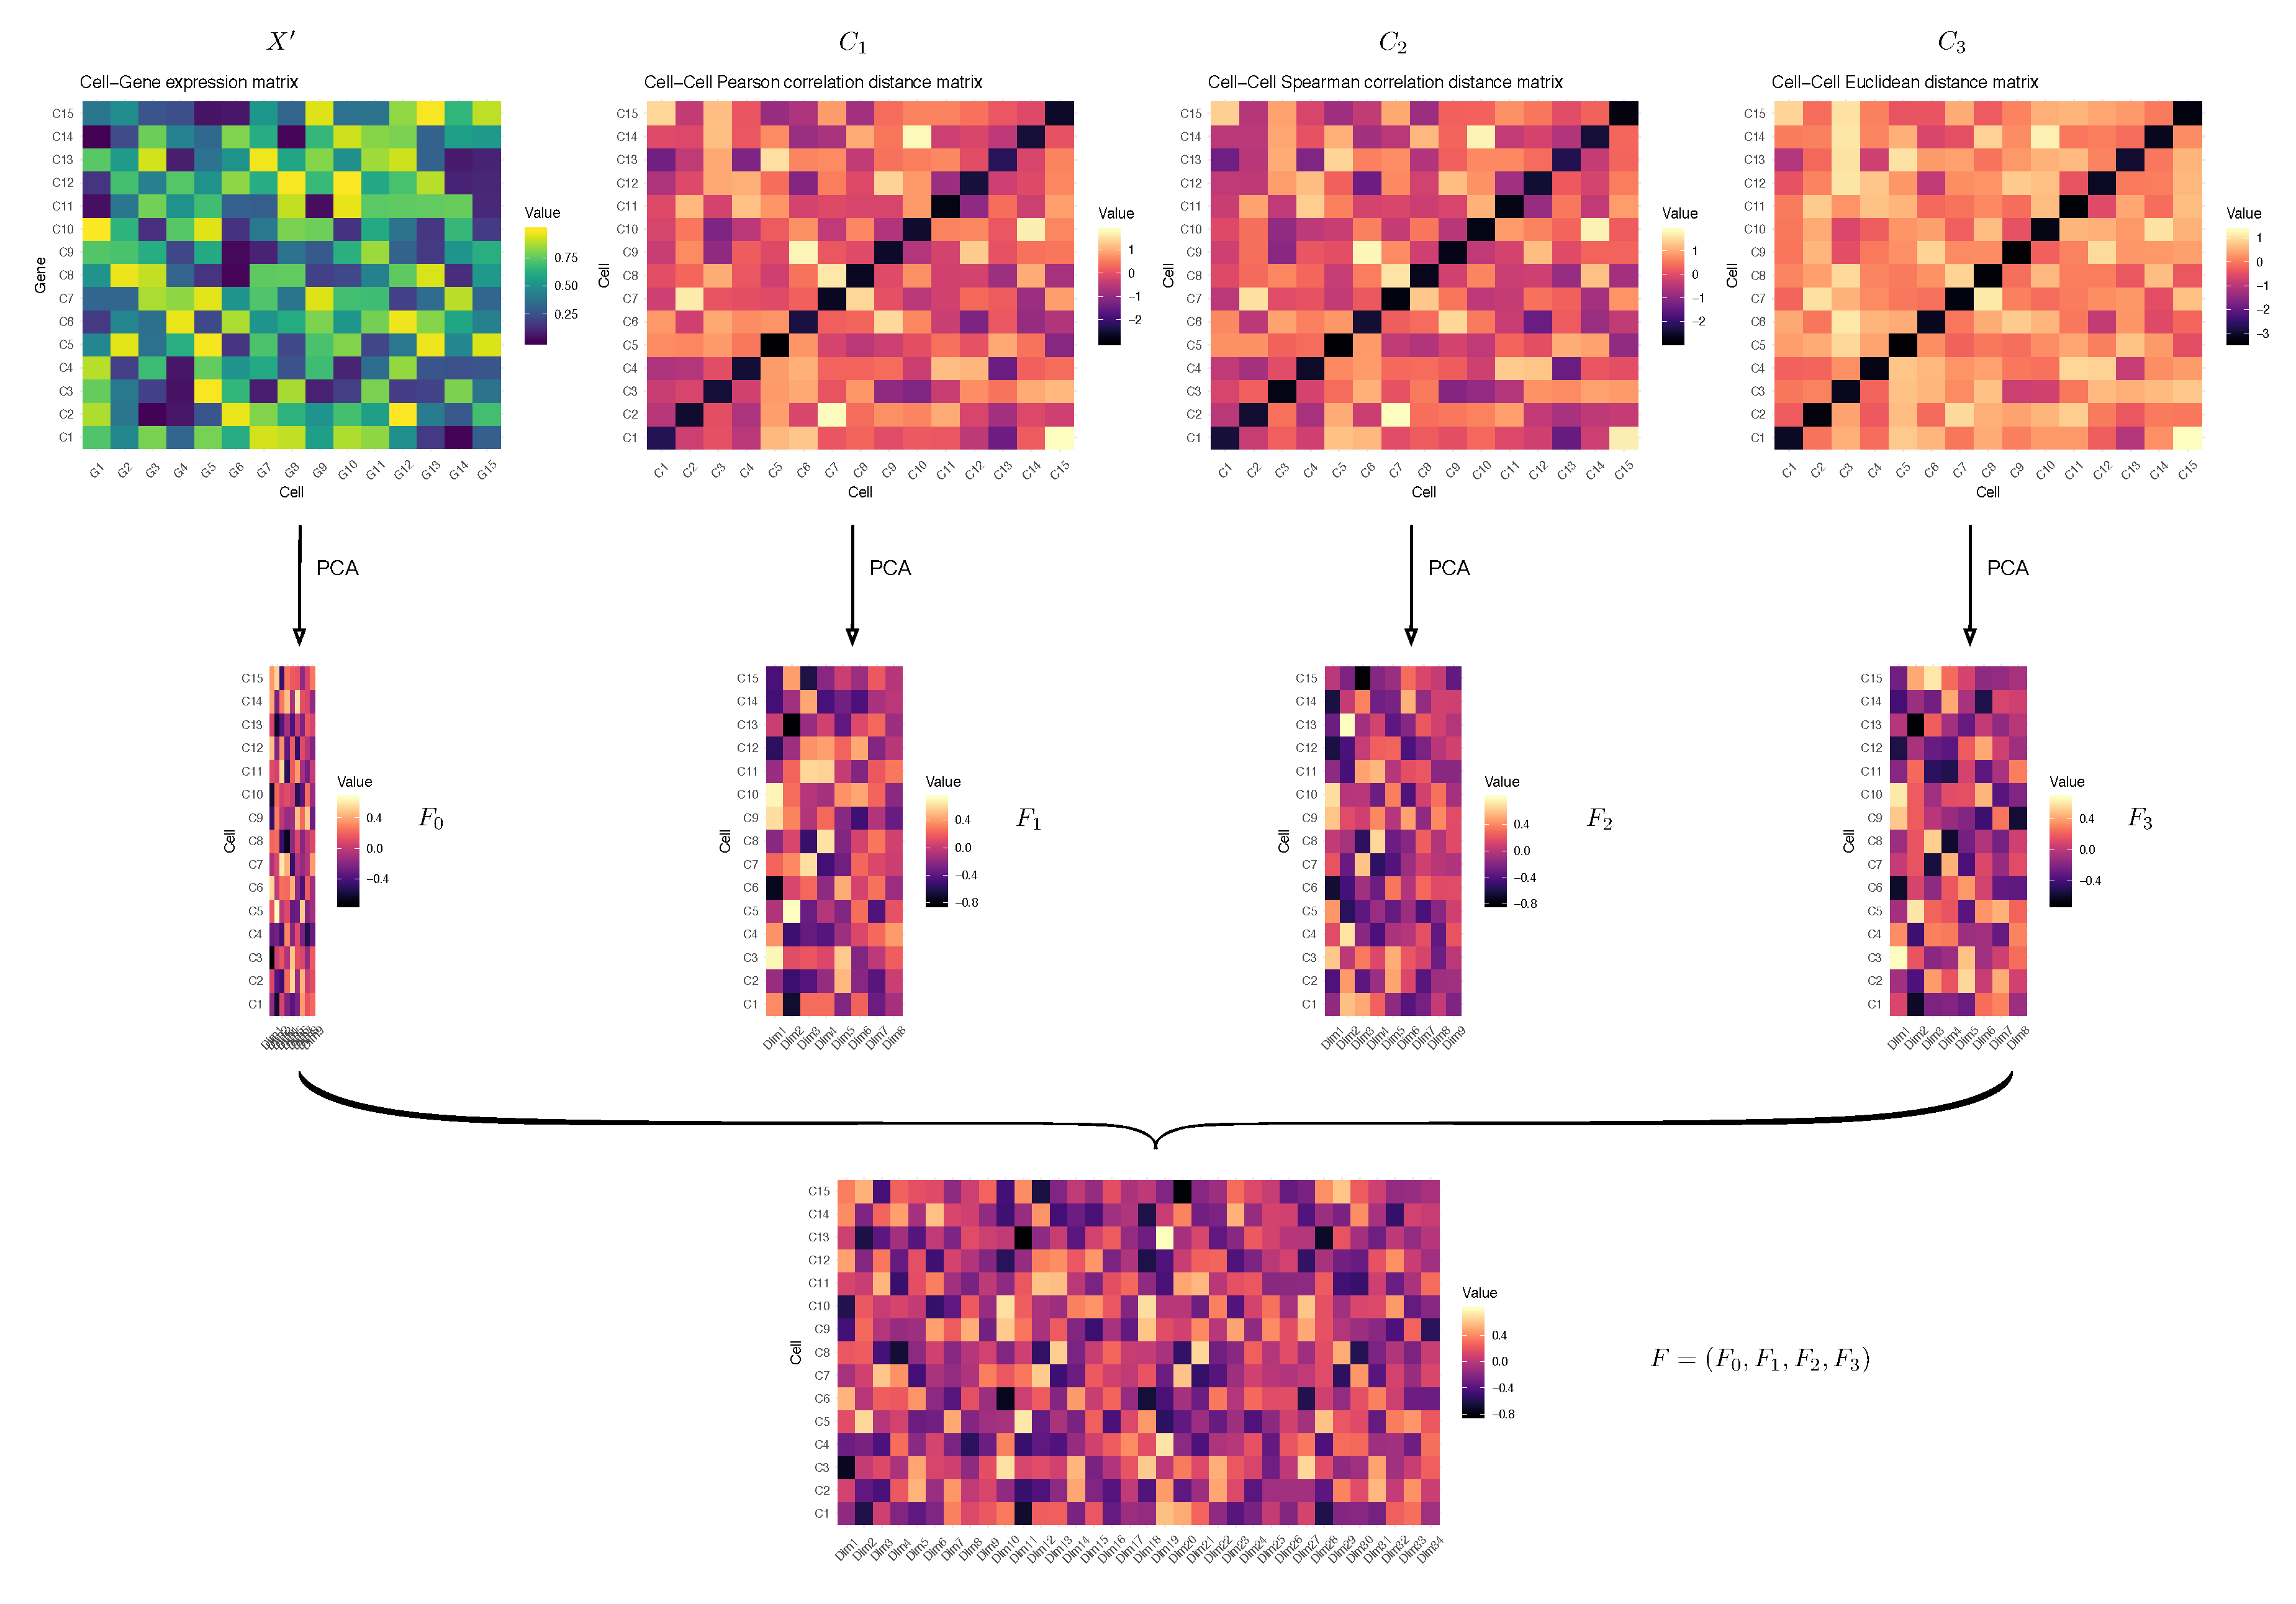
\includegraphics[width=0.9\textwidth]{rafsim.pdf}
    % \caption{Illustration of the hand-crafted feature matrix construction in a toy dataset with 15 cells and 15 genes. 
    % The final feature matrix $F$ is in a $15 \times 34$ shape in this case}
    \caption{
        一个有 15 个细胞和每个细胞 15 个基因的示例数据集中手动制作的特征矩阵构造。
        最终的特征矩阵 $F$ 在这个示例中是 $15\times34$ 维度大小的。
    }
    \label{fig:rafsim}
\end{figure}

RF (随机森林, Random Forest) 是一种应用非常广泛的基于决策树的分类和回归方法 \cite{breiman2001random}。
它也可以用无监督的方式来推断对象之间的相似性 \cite{shi2006unsupervised,breiman2011manual,pouyan2018random}。
基于 RF 的相似性学习方法很容易适应于并行计算,
对离群值具有鲁棒性,内在具有特征选择的特性,这三个特点特别适合用来分析高维和噪声数据,
特别是类似于单细胞 RNA 测序图谱数据。
我们按照以下步骤来学习细胞-细胞的相似性。
在选择一个单一的特征 $j$ (特征矩阵 $F$ 中的第 $j$ 列) 后, 
我们使用围绕质心点进行划分的算法 PAM (partitioning around medoids),估计类别的数量并得到对应于类别的伪标签。
与 K-means 聚类算法相比, PAM 对孤立点不敏感。
%我们直接使用 R 包 fpc \cite{package-fpc}中的 \textit{pamk} 函数来获取该特征 $j$ 的向量中的类标签。
然后,我们从 $F$ 中去掉第 $j$ 列,并且使用 RF 对缩减后的数据集 $F_{-j}$ 进行对伪标签的回归学习。
让 $f_p$ 表示 $F_{-j}$ 的第 $p$ 行,
如果 RF 包含 $N$ 颗树,并定义 $nt(f_p,f_q)$, 作为通过同一片叶子对细胞 $f_p$ 和 $f_q$ 进行归类的树的数量。
基于 RF 的 $n \times n$ 相似度矩阵 $S_j$ 是通过以下方式定义:
$S_{j_{pq}} = nt(f_p,f_q) / N, 1 \le p,q \le n$。
%我们使用 R 包 randomforest \cite{package-randomforest},其默认森林大小为 500 棵,即 $N=500$。
对所有的 $\tilde{p}$ 特征重复这个过程,得到 $\tilde{p}$ 相似度矩阵 $S_j$,$j=1,2,\ldots,\tilde{p}$。
通过对所有 $S_j$ 进行平均,得到最终的细胞-细胞相似度矩阵 $S$,
并通过 $D=1-S$ 得到距离矩阵 $D$。

接下来,对距离矩阵 $D$,使用层次聚类中的平均连锁聚类方法 (average linkage clustering) 来对细胞进行聚类,
使用了来自 R 包 dynamicTreeCut \cite{langfelder2007defining,package-dynamicTreeCut} 的 \textit{cutreeDynamic} 函数自动确定细胞的类别,
并为每个细胞分配正确的类标签。
另外,我们还提供了使用 R 包 dynamicTreeCut 中的 \textit{cutree} 函数来支持用户自定义细胞的类别数。

\subsubsection{差异基因分析}
\label{subsec:de}

使用 RafClust 得到了细胞的类别标签后,
我们采用 NODES \cite{Sengupta049734} 这一快速的非参数化、差异化表达 (DE) 分析工具进行差异基因分析。
NODES 被证明比传统的基于批量细胞测序的差异分析方法 DESeq2 \cite{love2014moderated}、edgeR \cite{robinson2010edger},
以及针对单细胞的差异表达分析方法 scde \cite{kharchenko2014bayesian} 和 Wilcoxon 秩和检验 (Wilcoxon rank sum test) 都有效 \cite{Sengupta049734}。
以 0.05 作为 FDR (False Discovery Rate) 的阈值, FC (fold change) 变化(也就是两个组间表达量的比值) 阈值默认为 log2(5)。
在 DE 基因中,在特定类中相对于其余各类显著上调的基因被命名为细胞类型特异基因。


\subsection{基于孤立森林的单细胞稀有细胞识别方法 DoRC}
\label{sec:method}

RaceID 和 GiniClust 都依靠无监督聚类来检测稀有细胞。
RaceID 中的 \textit{k}-means 聚类是基于距离的,
而 GiniClust 中的 DBSCAN 聚类是基于密度的。
它们都属于基于近邻的方法进行离群点检测。
基于近邻的方法假设一个离群样本与其最近邻的接近程度与该样本与数据集中大多数其它样本的接近程度有很大的差异。
聚类性能通常取决于一些参数敏感性且工作效率低下,因为不同分布的数据点之间的近似度不同。
另一个主要问题是,样本聚类的分辨率 (resolution) 问题。
一般来说,多级聚类变得至关重要,因为次要的类经常在首次筛选就被过滤掉了 \cite{campbell2017molecular}。
其它主要细胞类型会影响数据集中的表达差异,
特别是在处理大型 scRNA-seq 数据集时,情况变得更加糟糕。

为了解决上述问题,我们提出了一种从超大规模 scRNA-seq 数据中快速准确检测稀有细胞的方法,
命名为 DoRC。
DoRC 的灵感来自于我们观察到,稀有细胞在单细胞数据集里往往是``少而不同", 这跟机器学习里的样本孤立性十分契合。
孤立森林可以充分捕捉稀有细胞的特征,
其中,每个细胞的稀有性是以树枝的聚合长度为特征的。
一个细胞的聚合长度越长,该细胞与其它细胞区分的因素就越多,它成为稀有细胞的可能性就越大。
从数量上看,孤立森林中的聚合异常分数在本质上反应了稀有特性,
这为我们调查和进一步决定细胞的稀有性提供了基础。

DoRC 方法是用于从超大型 scRNA-seq 数据中发现稀有细胞,包括若干个子步骤,如图 \ref{fig:flowchart} 所示。
% \subsubsection{}
% \label{subsec:datapreprocessing} 
其中,预处理部分包括数据规范化和基因选择。
每个数据集上,在至少 3 个细胞中读数超过 2 的基因被保留用于下游分析,
然后使用中位数归一化。
除 \textit{Splatter\_500} 之外的其它数据集,
我们基于基于它们的相对分散度 (dispersion,即方差/均值) 与具有相似平均表达量的基因之间的预期分散度 \cite{zheng2017massively,macosko2015highly}选出 1000个变化最大的基因。
最后,将处理后的伪计数矩阵 (pseudo-count) 加 1 后进行对数变换。
对所有的数据集进行了预处理之后,后续的关键的处理步骤在下文中将详细讲述。

\begin{figure}[!htbp]
    \centering
    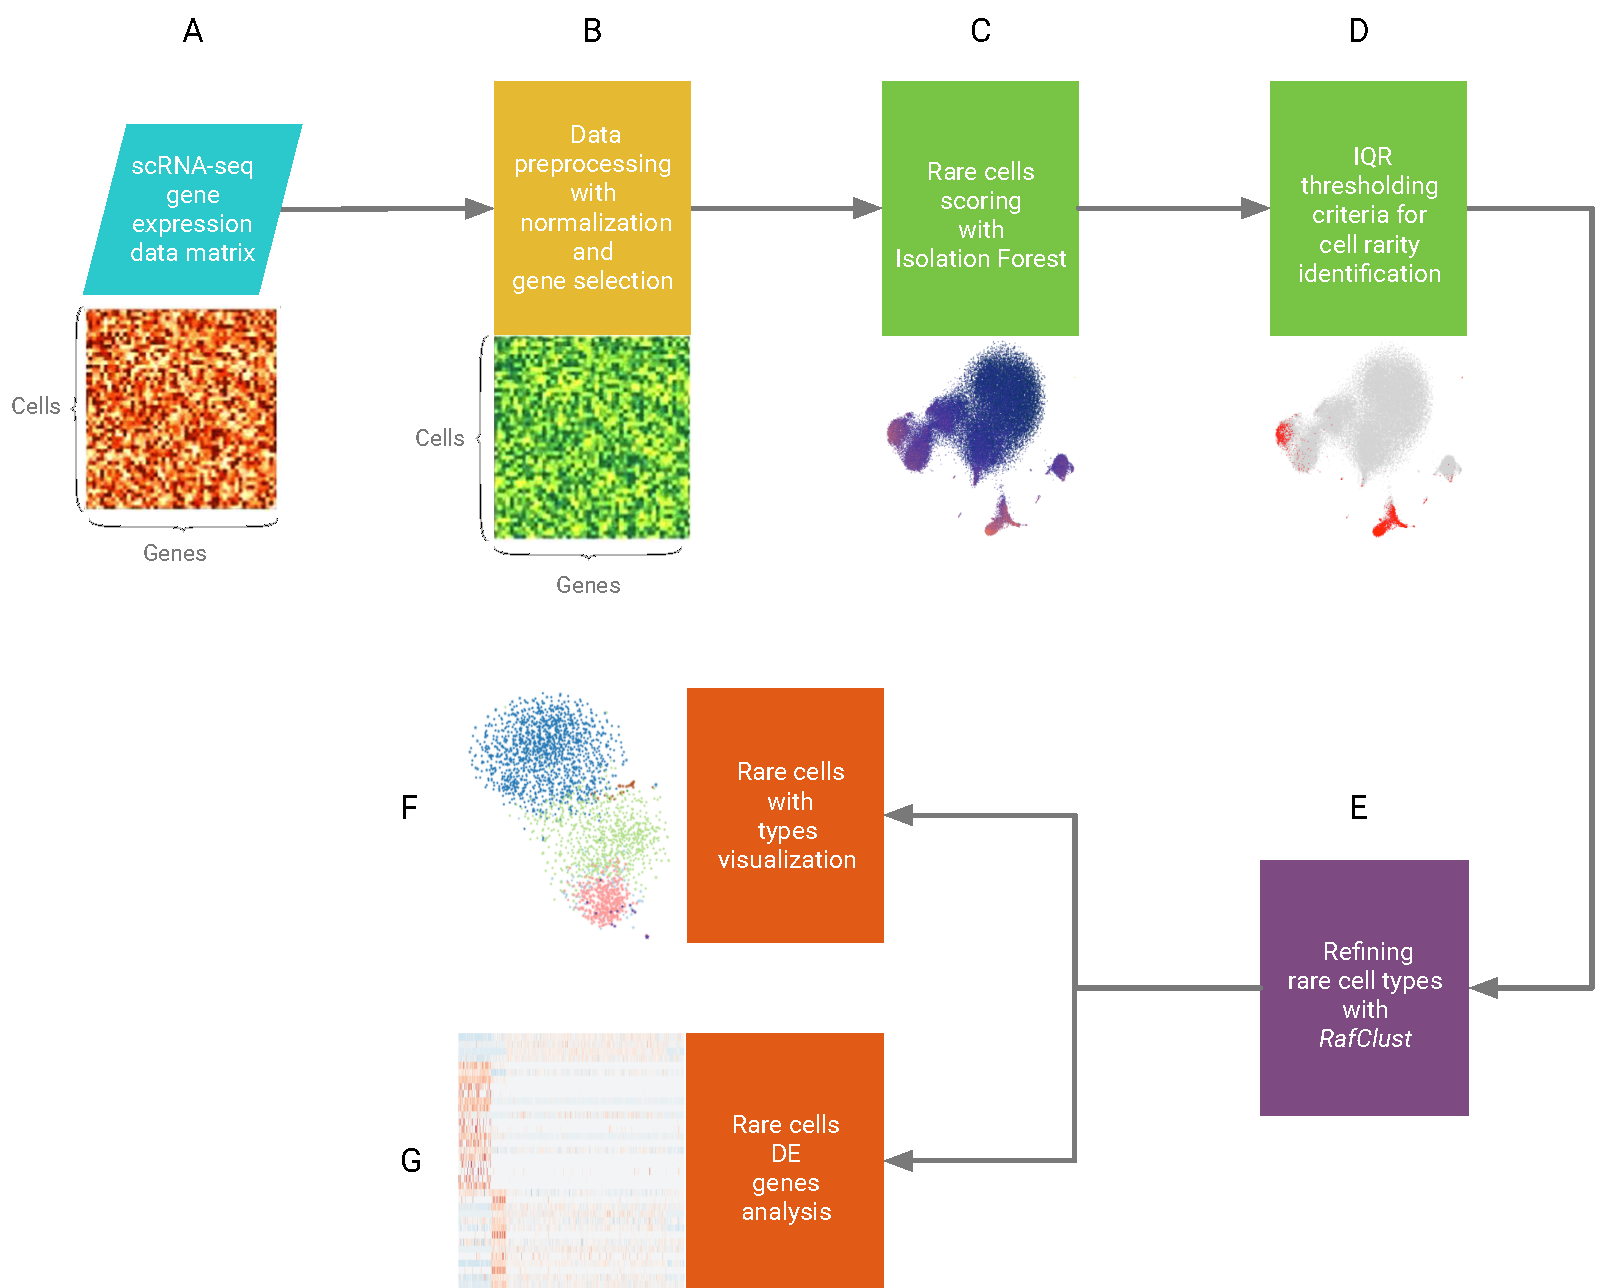
\includegraphics[width=\linewidth]{flowchartv4.pdf}
    % \caption{DoRC flowchart. The flowchart illustrates the processes of our proposed DoRC method for rare cells detection from ultra-large scRNA-seq data. 
    % Each annotated vignette in this figure represents the input or output visualization for the corresponding procedure. 
    % (A) The input is the scRNA-seq expression data 2D-matrix, whose row stands for cells, column for genes, respectively.
    % (B) Data preprocessing with the input expression data, the output is  a normalized and the column dimension reduced matrix. 
    % (C-D) Rare cells discovery with Isolation Forest, which are the workhorse procedures of DoRC. 
    % (C) Rare cells scoring with Isolation Forest, the output is a list of continuous anomaly scores for all the cells.
    % The scores can be visualized in the t-SNE-based 2D plot of the dataset; 
    % (D) IQR thresholding criteria for cell rarity identification, the binary annotations are also visualized in the t-SNE-based 2D plot.
    % (E) Refining rare cell types with RafClust. Notably, this sub-procedure is optional if we do not care about the types of rare cells.
    % (F) Rare cells with types visualization, different colors represent different rare cell types in the t-SNE-based 2D plot of the rare cells.
    % (G) Different expression genes analysis with different types of rare cells, the cell type specific genes are consequently obtained. 
    % }
    \caption{DoRC 流程图。该流程图展示了我们提出的从超大规模 scRNA-seq 数据中检测稀有细胞的过程。
    本图中的每个注释图代表了相应过程的输入或输出可视化。
    (A) 输入的是 scRNA-seq 表达数据二维矩阵,其中行代表细胞,列代表基因。
    (B) 用输入的表达数据进行数据预处理,输出的是一个归一化和列的维度缩减的矩阵。
    (C-D) 用 Isolation Forest 发现稀有细胞,这是 DoRC 的核心程序。
    (C) 用 Isolation Forest 进行稀有细胞评分,输出的是所有细胞的连续的异常得分向量。
    分数可以在基于 t-SNE 的数据集二维图中可视化。
    (D) 细胞稀有度识别的 IQR 阈值标准,二元标注也可以在基于 t-SNE 的二维图中可视化。
    (E) 用 RafClust 确定稀有细胞类型。值得注意的是,如果我们不关心稀有细胞的类型,这个步骤就不需要。
    (F) 稀有细胞与类型可视化,在基于 t-SNE 的稀有细胞二维图中不同的颜色代表不同的稀有细胞类型。
    (G) 对不同类型的稀有细胞进行不同的差异基因分析,从而得到细胞类型的特异基因。
    }
    \label{fig:flowchart}
\end{figure}

\subsubsection{使用孤立森林识别稀有细胞}
\label{subsec:if} 

孤立森林是一种无模型算法,它的计算效率很高,非常适合并行计算方法的使用 \cite{hariri2018batch}。
事实证明,它在检测异常方面也是非常有效的 \cite{susto2017anomaly}。
该算法的主要优越性在于,它并不依赖于为数据设置复杂的参数配置。
相反,它利用了异常数据``少而不同"的特点。
其它大多数异常检测算法 (anomaly detection algorithms) 都是通过了解异常数据的属性分布,并将其从其它正常数据样本中分离出来,从而找到异常数据 \cite{noto2010anomaly,chen2011ordinal,das2016incorporating}。
在孤立森林中结合树结构,从数据中抽取子样本,
并根据数据集中随机选取的特征值进行随机切割。
树枝路径越长,那么该样本为异常样本的可能性越低;
相反,路径越短的树枝越有可能是异常的。
因此,每个树枝的总长度可以被看作是对指定点的异常性衡量的``异常得分"。

孤立森林 \cite{liu2008isolation,liu2012isolation} 的算法思想同任何基于树结构的聚合 (ensemble) 方法一样,
也是在基于决策树结构之上的。
在训练时,给定一个维度为 $N$ 的数据集,
该算法选择一个随机的数据子样本来构建一棵二叉树。
树的分支过程通过选择一个随机维度 $x_i$,也就是一个单一的变量或特征来进行,其中 $i \in {1,2,\ldots,N}$。
如果一个给定的数据点在维度 $x_i$ 的值小于 $v$ ($v$ 是该维度中在最小值和最大值之间的随机值),
那么这个点就会被送到左分支;否则,就会走到右分支。
通过这种方式,树节点当前的数据被分割成两个子数据集。
这个分支过程在数据集上递归执行,直到一个点被隔离,或者达到预定的深度限制。
这个过程再次开始,用一个新的随机子样本来建立另一棵随机化树。
在建立大量的树的集合后,也就是一片森林,训练的过程就完成了。
在评分时,可以使用新的候选数据点或用于创建树的现有数据点。
根据指定点在每棵树中达到的深度,聚合的异常得分的计算等式是:
\begin{equation}
    \label{as}
    s(x,n) = 2^{-E(h(x))/c(n)}
\end{equation}
其中, $E(h(x))$ 是单个数据点 $x$ 在所有树中达到的深度的平均值, $h(x)$ 代表 $x$ 在树中的深度 (高度)。 
$c(n)$ 是归一化因子,定义为二叉搜索树 (BST) 中搜索失败的平均深度。
\begin{equation}
    \label{lab:as}
    c(n) = 2H(n - 1) - (2(n - 1)/n)
\end{equation}
其中 $H(i)$ 为谐波数,
可由 $ln(i) + 0.5772156649$ (欧拉常数) \cite{liu2012isolation}估计,$n$ 为建树时所用的数据点数。
$s(x,n)$ 的值接近 1 表示异常,远小于 0.5 表示正常观测值。
我们在这里使用的参数默认值与文献 \cite{liu2008isolation,liu2012isolation}一样,
即在所有实验中子样本数据为 256,树的集合数目为 100。

虽然用连续值来表示异常得分十分有意义,但有时关于细胞稀有度的二元标注可以极大地简化分析流程 (pipeline)。
因此,如果一个细胞的 DoRC 得分,即聚合异常得分,大于 $q_3 + 1.5 \times IQR$,则 DoRC 将其标记为罕见,
其中 $q_3$和 $IQR$ 分别表示所有细胞中 DoRC 分数的第三分位数和四分位数范围(第 75 百分位数$-$第 25 百分位数)。

\subsubsection{差异基因分析}
\label{subsec:de}

使用上一节中介绍的单细胞聚类方法 RafClust 得到了细胞的类别标签后,
我们采用 NODES \cite{Sengupta049734} 这一快速的非参数化、差异化表达 (DE) 分析工具进行差异基因分析。
NODES 被证明比传统的基于批量细胞测序的差异分析方法 DESeq2 \cite{love2014moderated}、edgeR \cite{robinson2010edger},
以及针对单细胞的差异表达分析方法 scde \cite{kharchenko2014bayesian} 和 Wilcoxon 秩和检验 (Wilcoxon rank sum test) 都有效 \cite{Sengupta049734}。
以 0.05 作为 FDR (False Discovery Rate) 的阈值, FC (fold change) 变化(也就是两个组间表达量的比值) 阈值默认为 log2(5)。
在 DE 基因中,在特定类中相对于其余各类显著上调的基因被命名为细胞类型特异基因。

\subsection{实验结果}

\subsubsection{聚类效果分析}
% \subsubsection{数据集}
% \label{subsec:datasets} 

为了测试 RafClust 在单细胞聚类场景下的性能,
我们使用了十个知名的 scRNA-seq 数据集上,细胞数目从小规模到中等规模不等。
每个数据集以第一作者的姓氏命名如下: 
Biase \cite{biase2014cell},
Treutlein \cite{treutlein2014reconstructing}, 
Pollen \cite{pollen2014low}, 
Kolod \cite{kolodziejczyk2015single}, 
Usoskin \cite{usoskin2015unbiased}, 
Darmanis \cite{darmanis2015survey}, 
Goolam \cite{goolam2016heterogeneity}, 
Li \cite{li2017reference},
Tasic \cite{tasic2016adult}, 
Zeisel \cite{zeisel2015cell}。
这十个数据集可以在 \url{https://hemberg-lab.github.io/scRNA.seq.datasets} 上获取, 
每个数据集的详情介绍如表 \ref{tbl:clusteringdatasets} 所示。

\begin{table}[!htbp]
  \centering
  \caption{
      %Overview of the  benchmark  datasets for the clustering performance comparison of RafClust with the other competing methods
      RafClust 与其它方法的聚类性能比较所使用的基准数据集概述
      }
  \label{tbl:clusteringdatasets}
  \resizebox{\columnwidth}{!}{%
  \begin{tabular}{llllrrrr}
  \toprule
  Dataset   &Accession 	&Sequencing protocol &Units &\#Cells &\#Genes	&\#Populations  & References \\
  \midrule
  Biase     &GSE57249     &SMARTer    &FPKM   &56	     &25 734     &5         &\cite{biase2014cell}\\
  Treutlein &GSE52583  	&SMARTer   	&FPKM  	&80      &23 271     &5 		&\cite{treutlein2014reconstructing}\\
  Pollen    &SRP041736 	&SMARTer   	&TPM   	&301     &23 730     &11 		&\cite{pollen2014low} \\
  %Patel     &GSE57872     &Smart-Seq 	&TPM   	&430     &5 948      &5			&\cite{patel2014single}\\
  Kolod     &E-MTAB-2600  &SMARTer    &CPM    &704     &38 616     &3         &\cite{kolodziejczyk2015single}\\
  Usoskin   &GSE59739  	&STRT-Seq  	&RPM   	&622     &25 334     &11 		&\cite{usoskin2015unbiased}\\
  Darmanis  &GSE67835  	&SMARTer    &CPM    &466     &22 088     &9         &\cite{darmanis2015survey}\\
  Goolam    &E-MTAB-3321  &Smart-Seq2	&CPM  	&124     &41 480     &5			&\cite{goolam2016heterogeneity}\\
  Li     	  &GSE81861  	&SMARTer    &CPM   &561     &55 186      &9         &\cite{li2017reference}\\
  Tasic     &GSE71585     &SMARTer    &RPKM   &1 679   &24 057     &18        &\cite{tasic2016adult}\\
  Zeisel    &GSE60361     &STRT-Seq  	&UMI   	&3 005   &19 972     &9			&\cite{zeisel2015cell}\\
  \bottomrule                   
  \end{tabular}
  }
\end{table}


% \subsubsection{评价指标}
聚类的效果是使用真实的类别标签 $L_T$ 和估计的类别标签 $L_E$ 之间的相似性来衡量,
使用的是调整后的 Rand 指数 (Adjusted Rand index, ARI) \cite{hubert1985comparing,wu2005dynamic}:
\begin{equation}
\label{eq:ARI}
\resizebox{0.8\textwidth}{!}{$
    ARI(L_E,L_T)=\frac{\sum_{}{}_{e,t} \begin{pmatrix}n_{et}\\ 2\end{pmatrix} - \begin{bmatrix}  \sum_{}{}_{e} \begin{pmatrix}n_{e}\\ 2\end{pmatrix}\sum_{}{}_{t} \begin{pmatrix}n_{t}\\ 2\end{pmatrix}  \end{bmatrix} / \begin{pmatrix}n\\ 2\end{pmatrix} 
    }{\frac{1}{2}\begin{bmatrix}
    \sum{}{}_e\begin{pmatrix}n_{e}\\ 2\end{pmatrix} + \sum{}{}_t\begin{pmatrix}n_{t}\\ 2\end{pmatrix}
    \end{bmatrix} - \begin{bmatrix}
    \sum{}{}_e\begin{pmatrix}n_{e}\\ 2\end{pmatrix} \sum{}{}_t\begin{pmatrix}n_{t}\\ 2\end{pmatrix} 
    \end{bmatrix}/\begin{pmatrix}n\\ 2\end{pmatrix}}    
$}
\end{equation}
其中 $n$ 是单细胞的总个数, 
$n_e$ 和 $n_t$ 分别是估计的类别 $e$ 和真实的类别 $t$ 中的单细胞数目; 
并且 $n_{et}$ 是估计的类别 $e$ 和真实的类别 $t$ 共有的单细胞的数目。
ARI 的范围是 -1 到 1 ,其中 1 表示估计的聚类与真实的聚类完全相同。
如果一个算法的 ARI 值越高,那么该方法的聚类效果就越好。

% \subsubsection{实验结果分析}

为了测试 RafClust 的性能,
我们将其应用在十个知名的 scRNA-seq 数据集上 (数据详情见表 \ref{tbl:clusteringdatasets}),
将其 ARI 值与其它六种方法进行比较,
包括 RaceID2 \cite{grun2016novo}, CIDR \cite{lin2017cidr}, SIMLR \cite{wang2018simlr}, SAFE \cite{yang2018safe}, RtsneKmeans \cite{hartigan1979algorithm,maaten2008visualizing,van2014accelerating}, RAFSIL \cite{pouyan2018random}。
这六种聚类方法均以 R 包的形式实现并公开了代码,它们的概述如表 \ref{supp-tbl:clustereringmethods} 所示。
通过将每种方法的聚类结果与每个基准数据集的细胞类型注释进行比较,计算出对应的 ARI 值。 
由于个别方法在代码中引入了随机函数和随机种子,使得运行结果有一定的随机性。
因此我们在每个数据集上对每个方法重复运行 5 次,结果中位数的 ARI 值如图 \ref{fig:rafari} 所示。
由图 \ref{fig:rafari} 可知, RafClust 在 ARI 上优于其它六种方法。
我们还记录了这个对比实验每个方法在每个数据集上的执行时间 (图 \ref{fig:running-detail}),并将平均执行时间与其它基准方法进行比较,结果如图 \ref{fig:running-summary} 所示。
该实验是在运行 GNU Linux/Ubuntu 16.04 操作系统与 4.15.0-46-generic 内核的工作站上进行的,
硬件配置如下: Intel(R) Xeon(R) CPU E5-2630 v4 @ 2.20GHz, 40 个核心, 256GB 内存。
由图 \ref{fig:running-summary} 可知, RafClust 针对细胞规模从小型到中型的 scRNA-seq 数据集在计算效率上是可以接受的。
RafClust 的 R 包可在 GitHub 仓库 \url{https://github.com/chenxofhit/RafClust} 上下载和使用,
本节相关的实验代码和相关数据集可以根据读者的要求提供。


\begin{table}[!htbp]
  \centering
  \caption{
  %Overview of the benchmark clustering methods
  使用的聚类方法概览
  }
  \label{supp-tbl:clustereringmethods}
  \resizebox{\columnwidth}{!}{%
      \begin{tabular}{lll}
      \toprule
      Method                                                                     & Description                                                                                                                                                        & Reference \\
      \midrule
      CIDR (v0.1.5)                                                              & PCA dimension reduction based on zero-imputed similarities, followed by hierarchical clustering                                                                    & \cite{lin2017cidr}         \\
      \begin{tabular}[c]{@{}l@{}}RaceID2 (March 3, \\ 2017 version)\end{tabular} & K-medoids clustering based on Pearson correlation dissimilarities                                                                                                  & \cite{grun2016novo}        \\
      RtsneKmeans                                                                & \begin{tabular}[c]{@{}l@{}}t-SNE dimension reduction (initial PCA dim=50, t-SNE dim=3, perplexity=30) and K-means \\ clustering with 25 random starts\end{tabular} & \cite{hartigan1979algorithm, maaten2008visualizing,van2014accelerating}        \\
      SAFE (v2.1.0)                                                              & Ensemble clustering using SC3, CIDR, Seurat and t-SNE + K-means                                                                                                     & \cite{yang2018safe}         \\
      SIMLR                                                                      & An appropriate cell to cell distance metric by multi-kernel learning, followed by spectral clustering                                                                                                                                                          & \cite{wang2018simlr}         \\
      RAFSIL                                                                     & Random forest based cell to cell similary learning, followed by K-means or hierarchical clustering                                                                                                                                                              & \cite{pouyan2018random}        \\
      \bottomrule
  \end{tabular}
  }
\end{table}

\begin{figure*}[!htbp]
    \centering
    \begin{minipage}[b]{0.45\linewidth}
      \centering
      \centerline{
        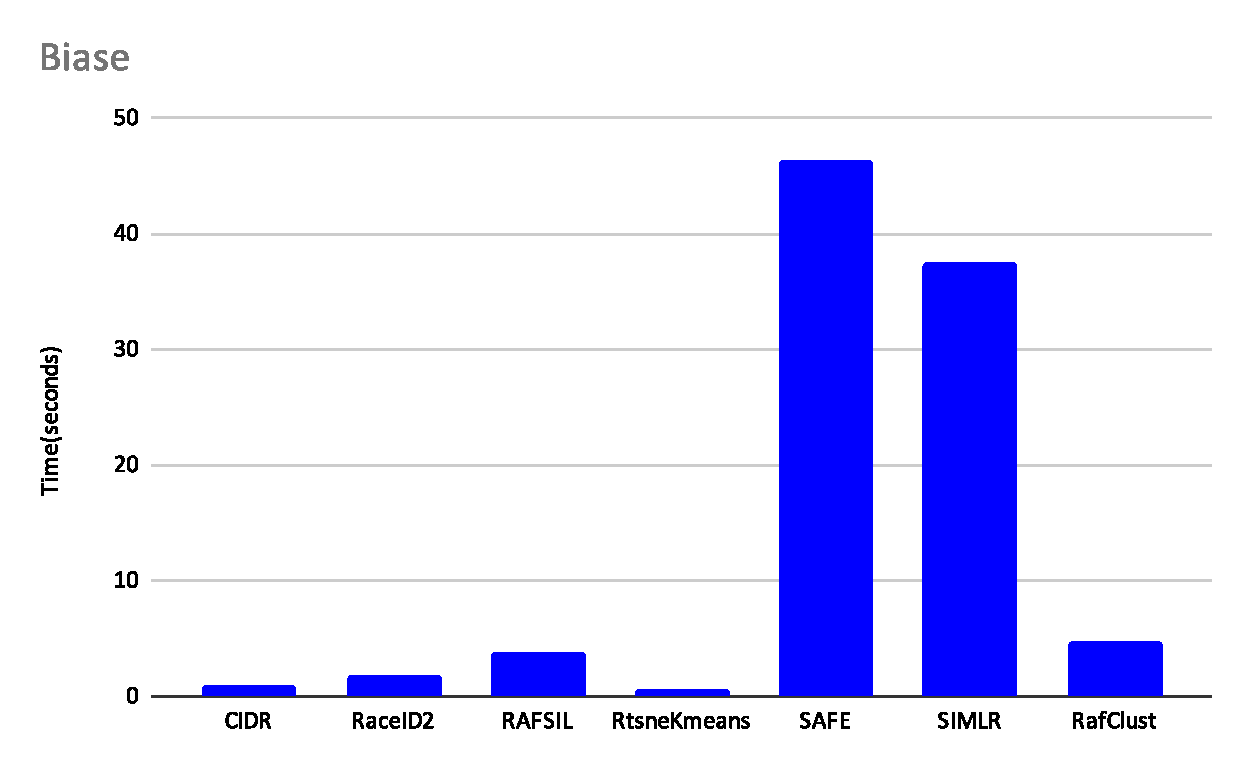
\includegraphics[width = \linewidth]{Biase.pdf}}
      \medskip  
    \end{minipage}
    \begin{minipage}[b]{0.45\linewidth}
      \centering
      \centerline{
        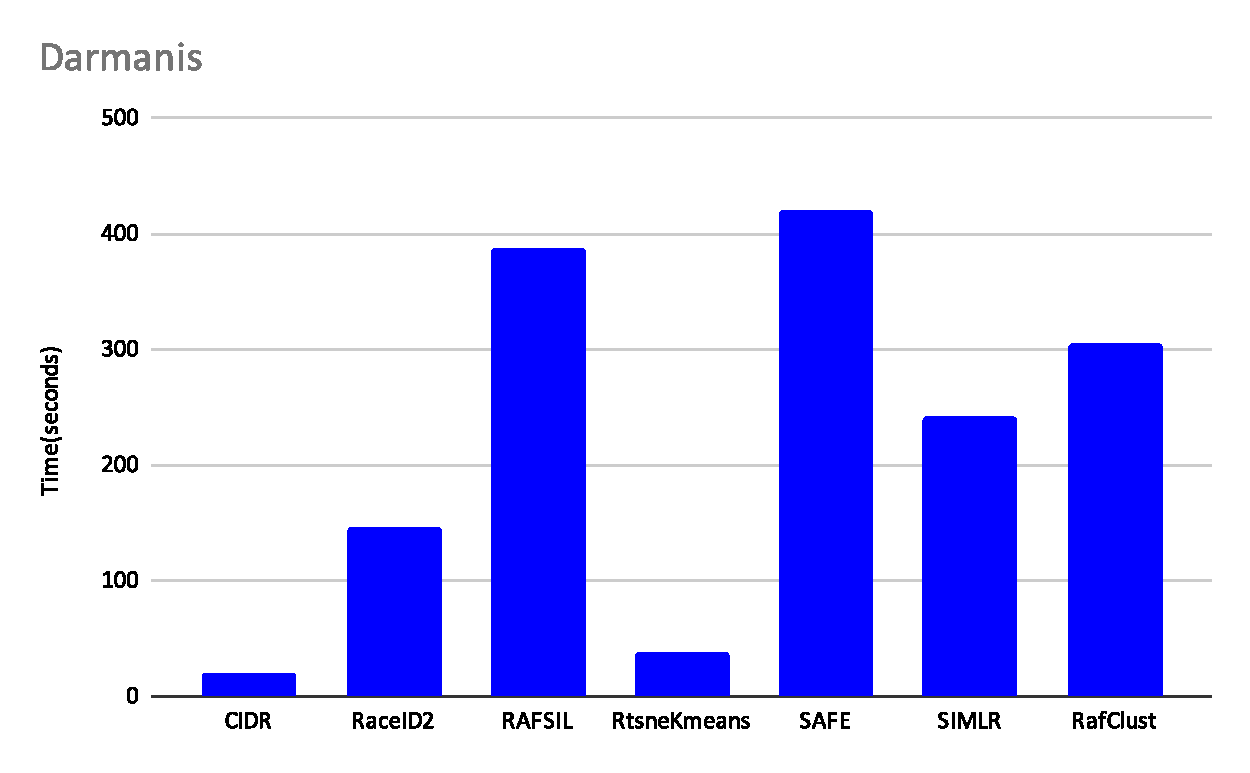
\includegraphics[width =\linewidth]{Darmanis.pdf}}
      \medskip  
    \end{minipage}
      \begin{minipage}[b]{0.45\linewidth}
      \centering
      \centerline{
        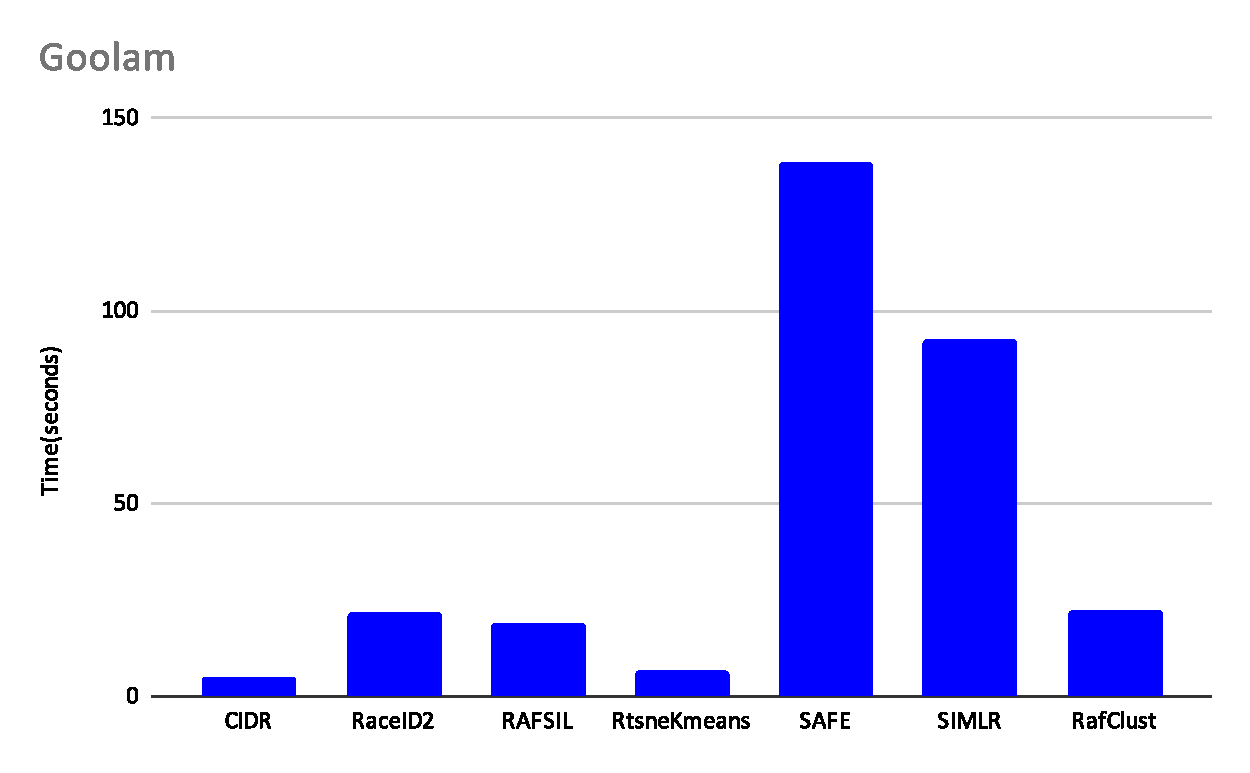
\includegraphics[width = \linewidth]{Goolam.pdf}}
      \medskip  
    \end{minipage}
    \begin{minipage}[b]{0.45\linewidth}
      \centering
      \centerline{
        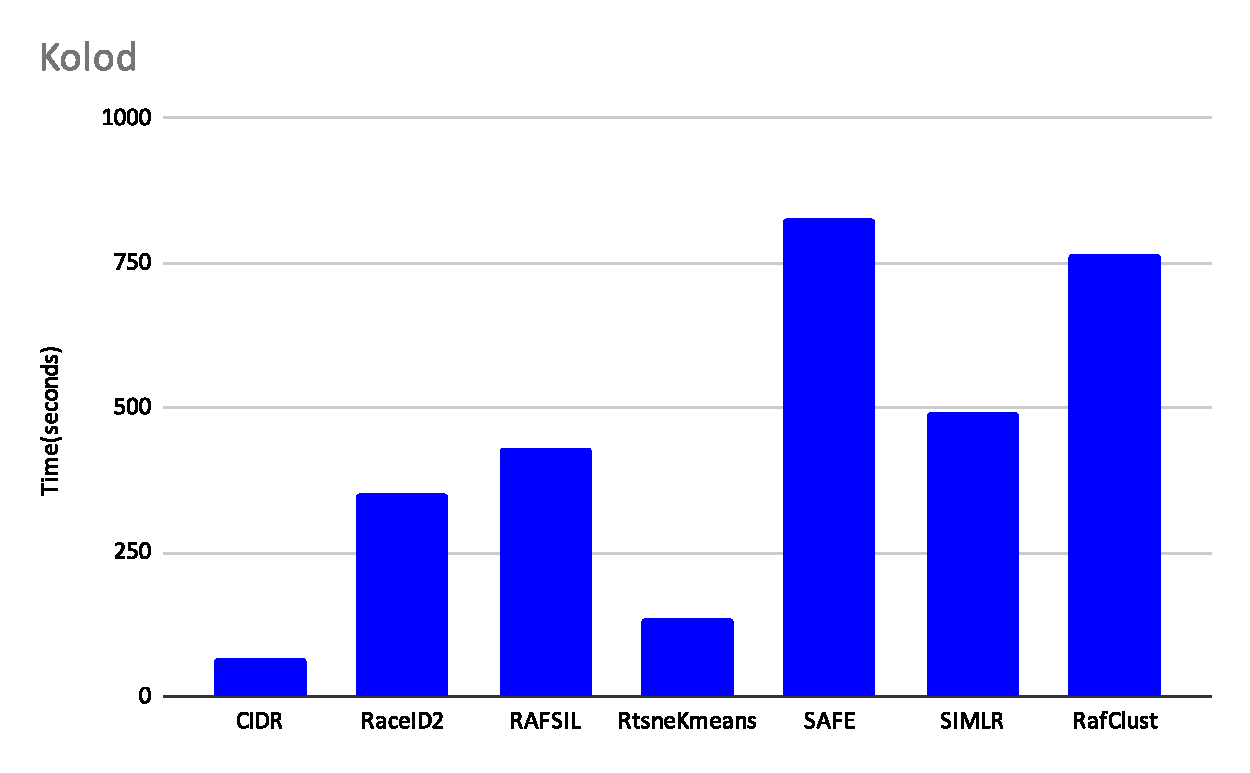
\includegraphics[width =\linewidth]{Kolod.pdf}}
      \medskip  
    \end{minipage}
    \begin{minipage}[b]{0.45\linewidth}
        \centering
        \centerline{
          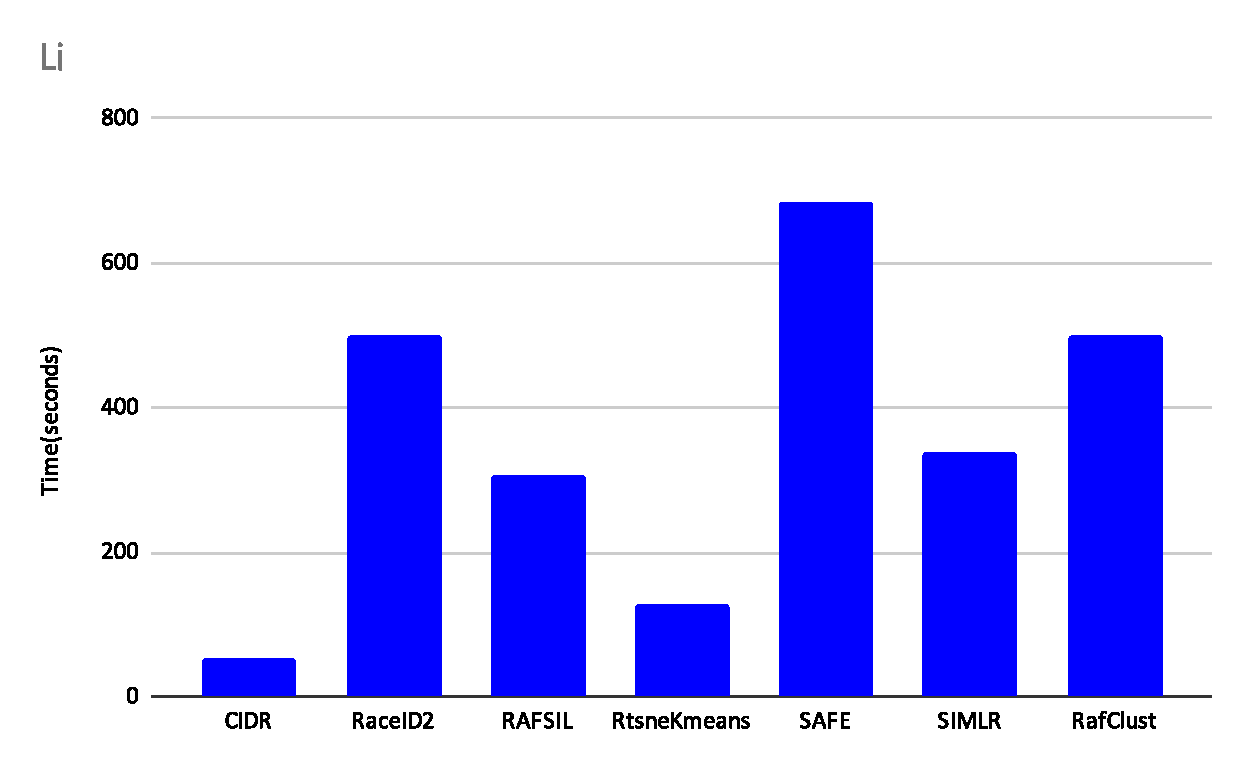
\includegraphics[width =\linewidth]{Li.pdf}}
        \medskip  
      \end{minipage}
      \begin{minipage}[b]{0.45\linewidth}
        \centering
        \centerline{
          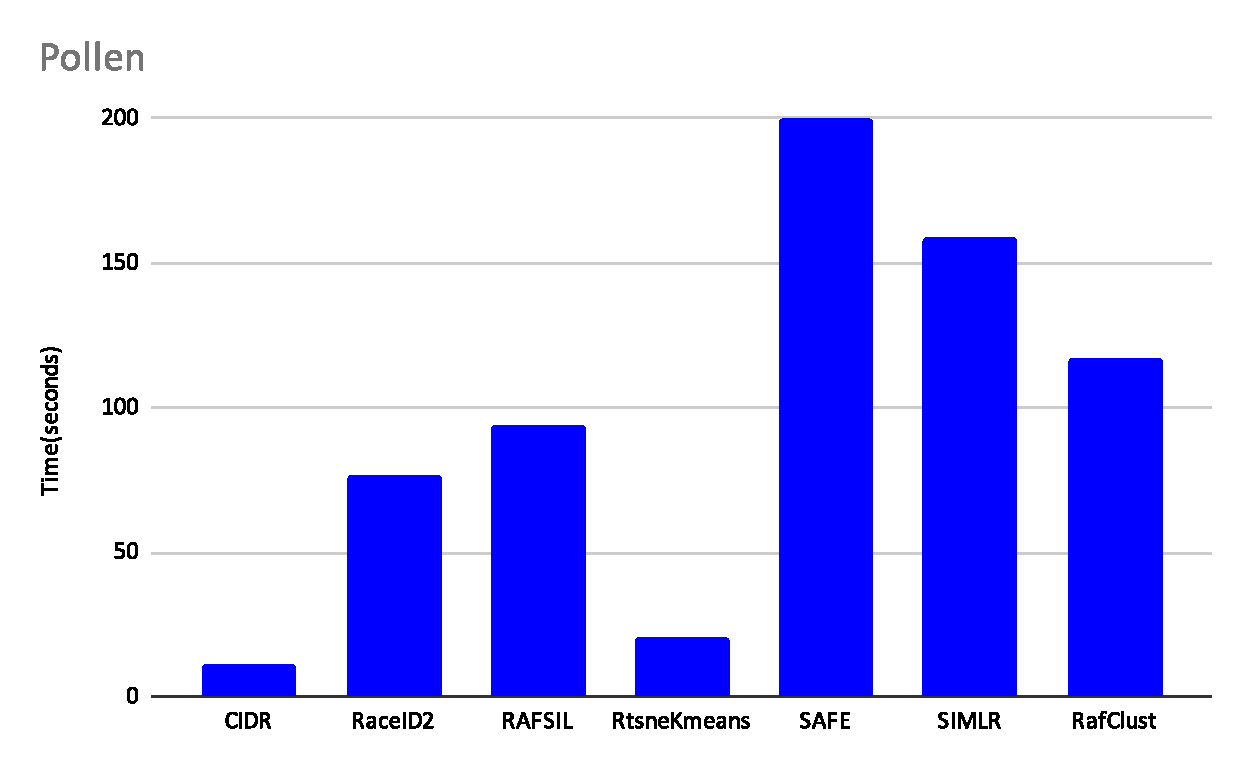
\includegraphics[width =\linewidth]{Pollen.pdf}}
        \medskip  
      \end{minipage}
      \begin{minipage}[b]{0.45\linewidth}
        \centering
        \centerline{
          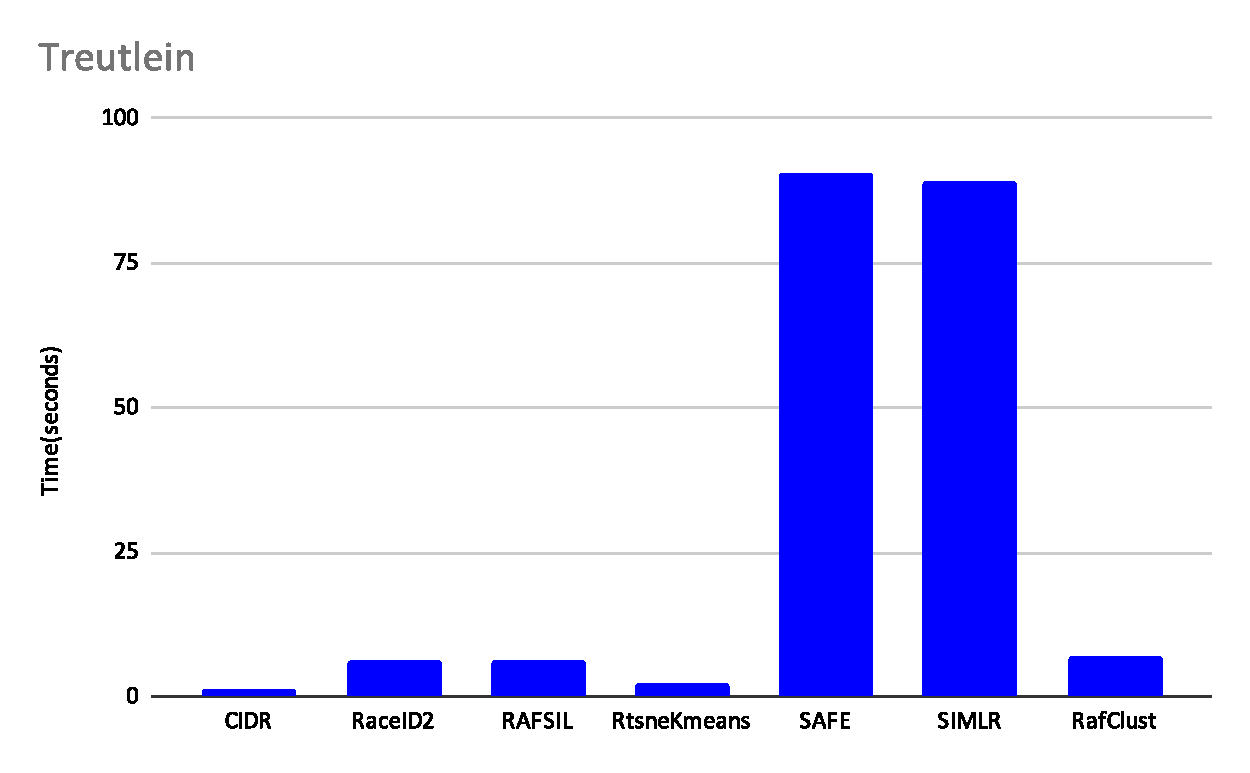
\includegraphics[width =\linewidth]{Treutlein.pdf}}
        \medskip  
      \end{minipage}
      \begin{minipage}[b]{0.45\linewidth}
        \centering
        \centerline{
          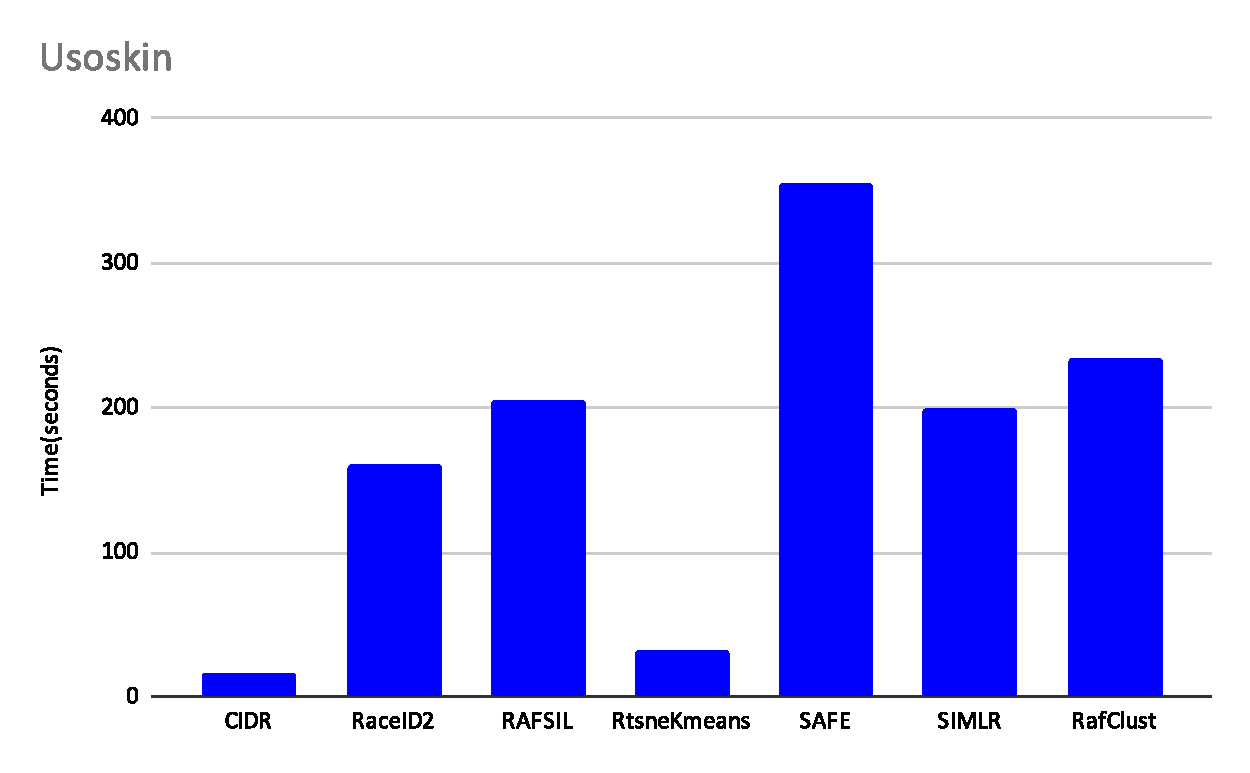
\includegraphics[width =\linewidth]{Usoskin.pdf}}
        \medskip  
      \end{minipage}
      \begin{minipage}[b]{0.45\linewidth}
        \centering
        \centerline{
          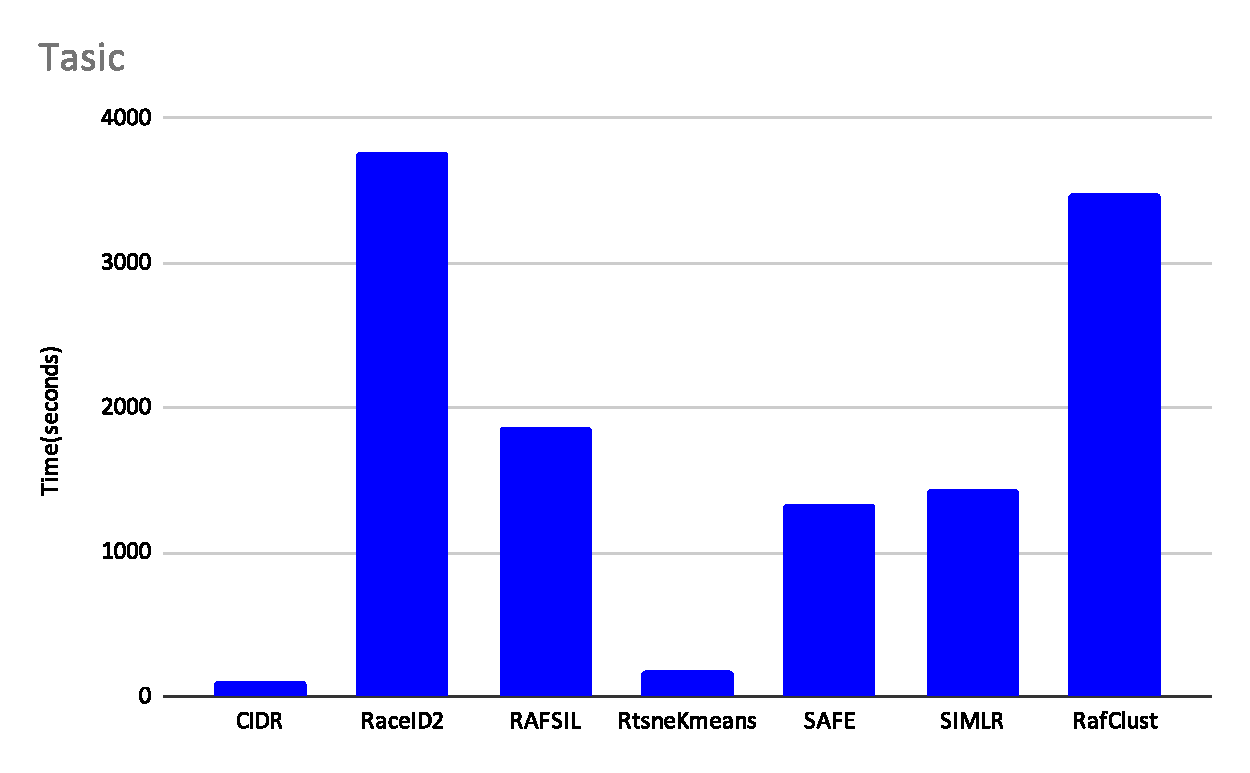
\includegraphics[width =\linewidth]{Tasic.pdf}}
        \medskip  
      \end{minipage}
      \begin{minipage}[b]{0.45\linewidth}
        \centering
        \centerline{
          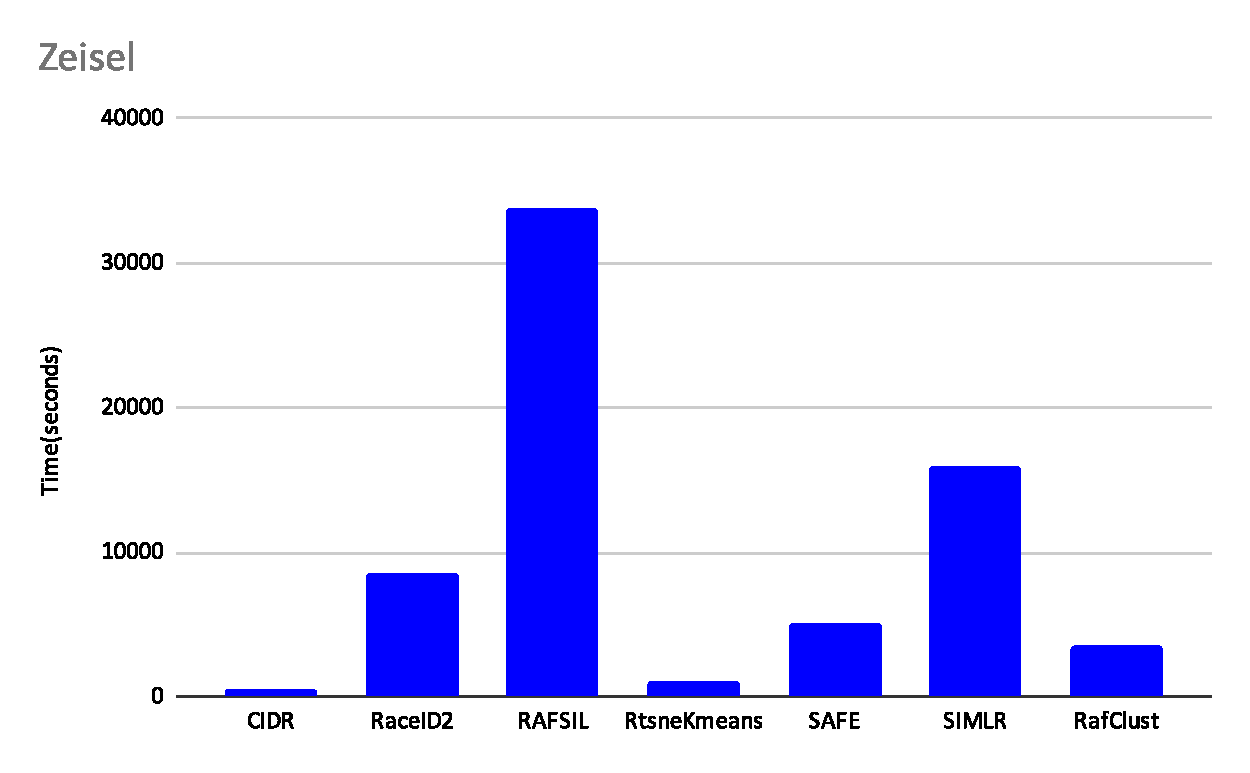
\includegraphics[width =\linewidth]{Zeisel.pdf}}
        \medskip  
      \end{minipage}
    \caption{
    RafClust 与其它六种方法在 10 个数据集上的中位数运行时间示意图。
    }
    \label{fig:running-detail}
    \vspace{-0.5em}
  \end{figure*}
 
  \begin{figure}[!htbp]
    \centering
    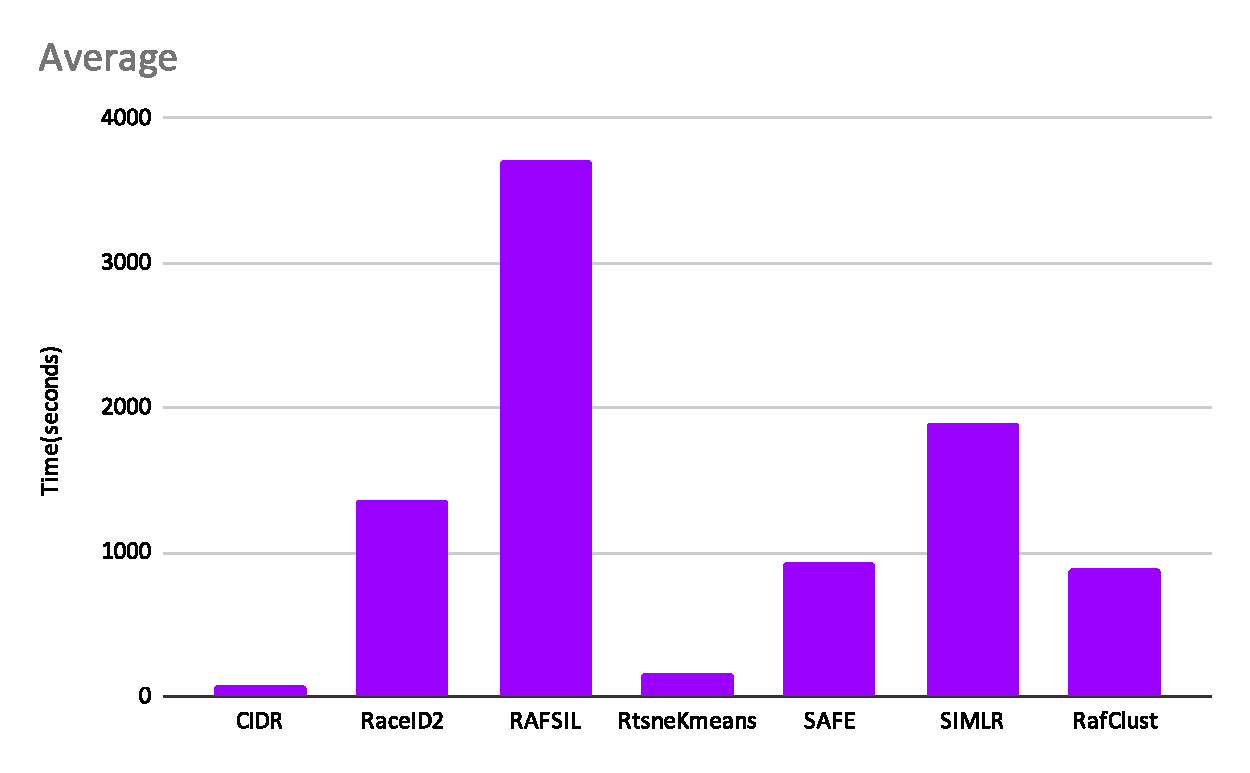
\includegraphics[width=0.9\textwidth]{Average.pdf}
    \caption{
    RafClust 与其它六种方法在 10 个数据集上的中位数运行时间示意图。
    }
    \label{fig:running-summary}
\end{figure}

\begin{figure}[!htbp]
    \centering
    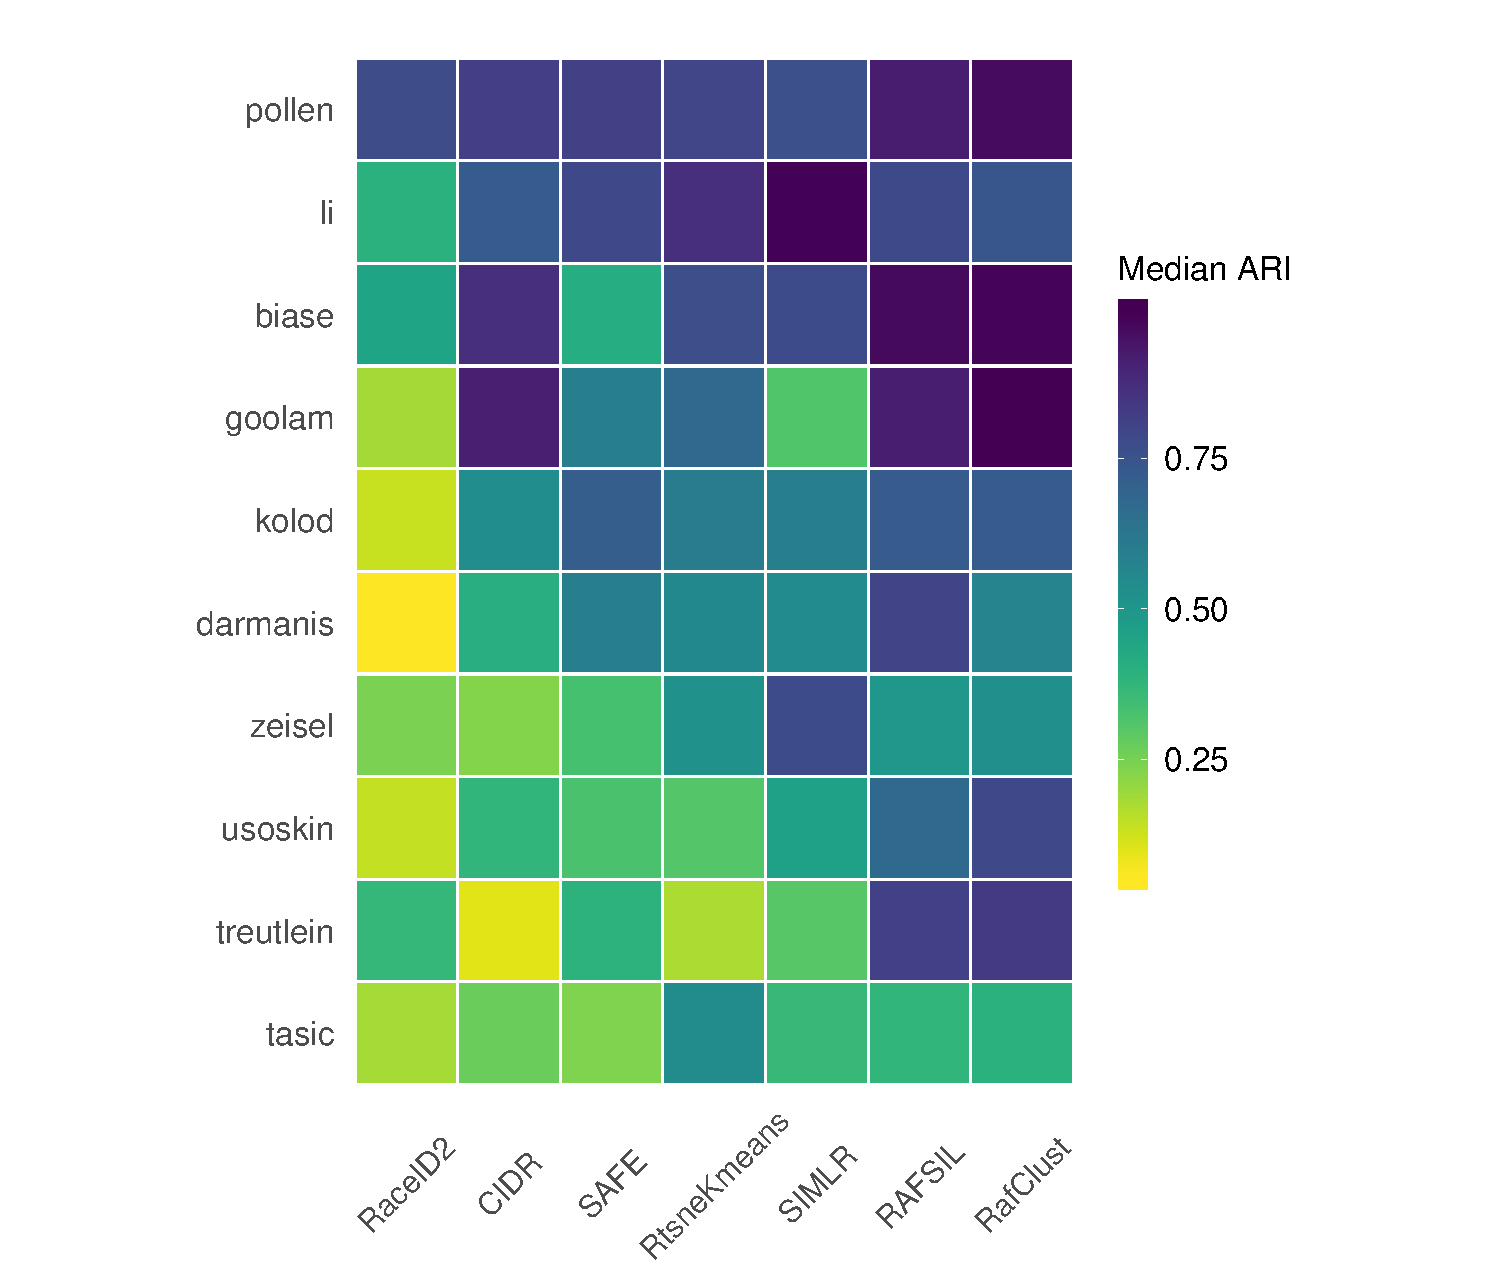
\includegraphics[width=0.9\textwidth]{Figure_ari_summary.pdf}
    \caption{
    % Median ARI across different runs on the same dataset for the methods
    不同数据集上不同方法的 ARI 中位数结果,颜色越深表示 ARI 中位数值越高。
    }
    \label{fig:rafari}
\end{figure}

在这十个数据集上,我们选择了 Goolam 和 Usoskin 两个数据集进行了数据集和聚类结果可视化。
从图 \ref{fig:rafari} 可知 SIMLR、RAFSIL 这两种方法的 ARI 仅次于方法 RafClust,
因此我们选用它们跟 RafClust 对比,在这两个数据集上对聚类结果进行了可视化, 
如图 \ref{fig:goolam-tsne} 和 \ref{fig:usoskin-tsne} 所示。
总体上来看, SIMLR 和 RAFSIL 均比原始数据上直接进行 t-SNE 结果要好,
但是 RafClust 表现比 SIMLR、RAFSIL 这两种方法结果要好。

\begin{figure}[!htbp]
  \centering
  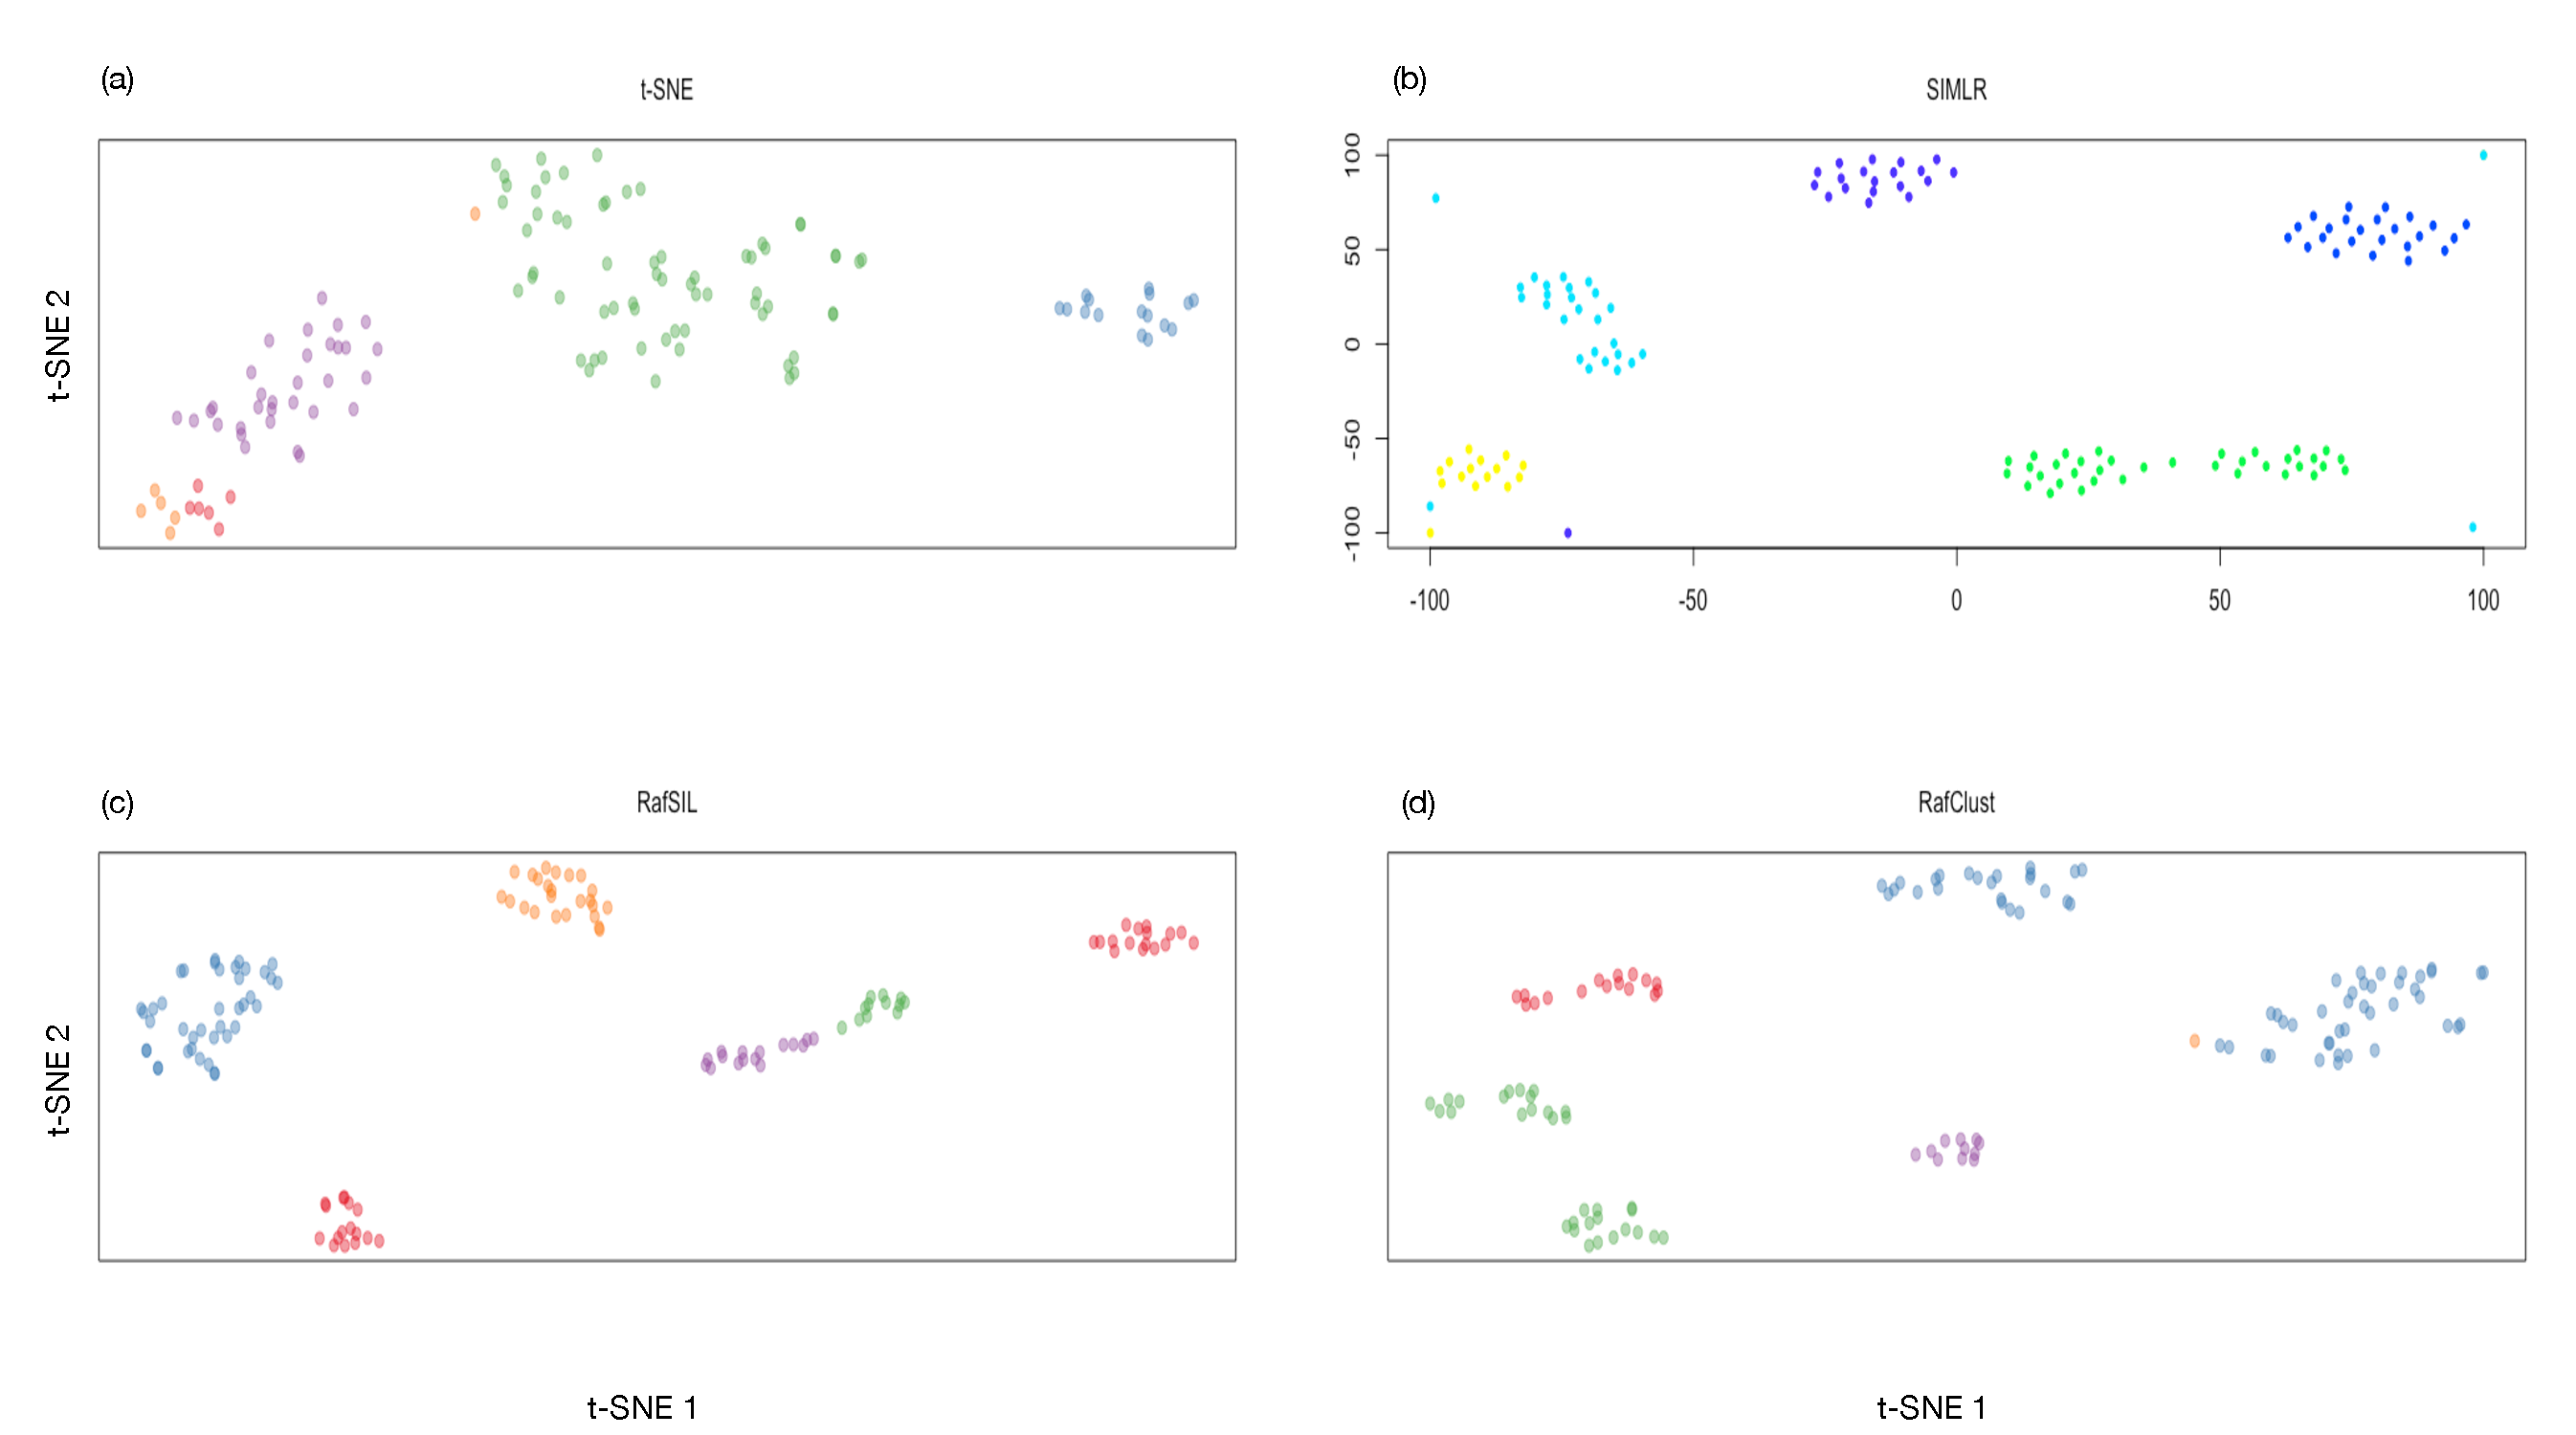
\includegraphics[width=\linewidth]{goolam-tsne.pdf}
  \caption{
  Goolam 数据集上的可视化。
  (a) 原始数据集使用 t-SNE 可视化,使用了真实的细胞类别标签进行着色,参数 perplexity 设置为 20。
  (b)  SIMLR 方法聚类结果可视化。
  (c)  RAFSIL 方法聚类结果可视化,参数 perplexity 设置为 20。
  (d)  RafClust 方法聚类结果可视化,对距离矩阵使用 t-SNE 进行可视化,参数 perplexity 设置为 20。
  }
  \label{fig:goolam-tsne}
\end{figure}


\begin{figure}[!htbp]
  \centering
  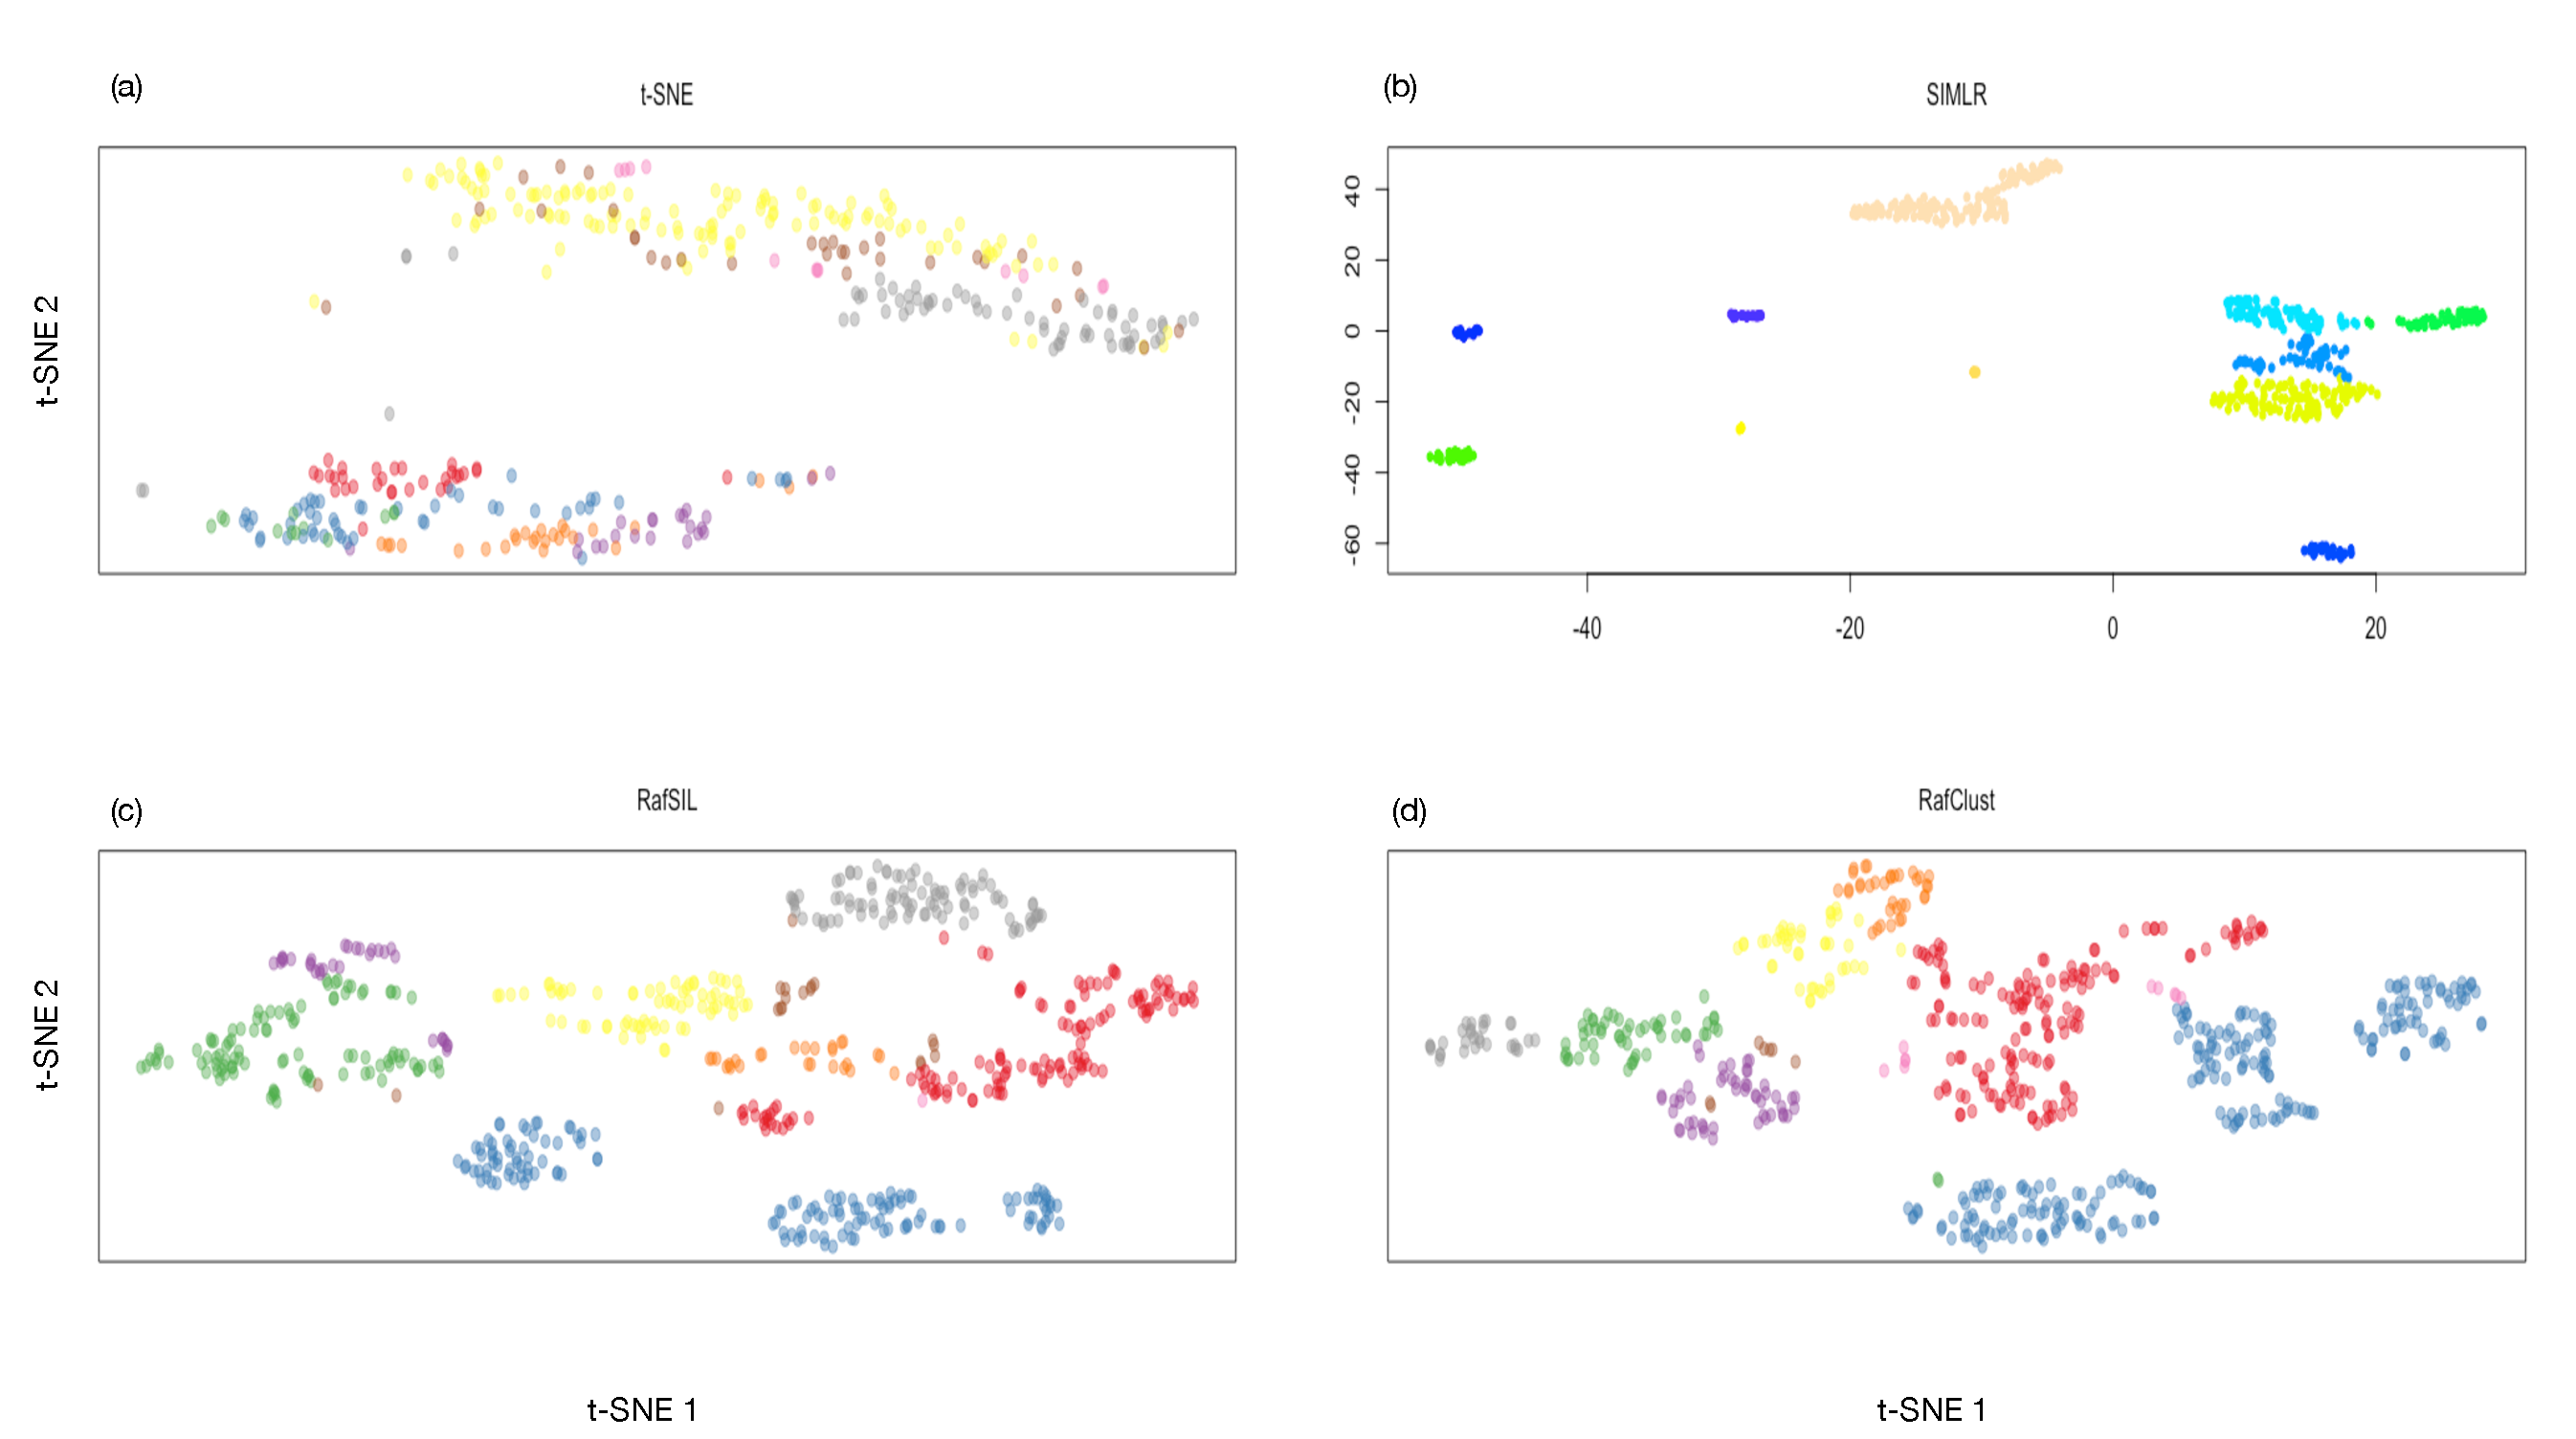
\includegraphics[width=\linewidth]{usoskin-tsne.pdf}
  \caption{
  Usoskin 数据集上的可视化。
  (a) 原始数据集使用 t-SNE 可视化,使用了真实的细胞类别标签进行着色,参数 perplexity 设置为 20。
  (b)  SIMLR 方法聚类结果可视化。
  (c)  RAFSIL 方法聚类结果可视化,参数 perplexity 设置为 20。
  (d)  RafClust 方法聚类结果可视化,对距离矩阵使用 t-SNE 进行可视化,参数 perplexity 设置为 20。
  }
  \label{fig:usoskin-tsne}
\end{figure}


% \subsection{DoRC 方法的实验结果}

% \subsubsection{数据集}
% \label{subsec:datasets} 

% 第一个数据集 \textit{PBMCs\_68k}由 68579 个从健康供体收集的 PBMCs 组成 \cite{zheng2017massively}。
% 11 个纯化的 PBMCs 亚群的单细胞表达谱被用作细胞类型标签的参考。
% 该数据集可在 \url{www.10xgenomics.com} 下载。

%第二个数据集textit{MSE/20k}包含了来自小鼠大脑Arc-ME区域周围的 ${sim} 20$k scRNA-seq图谱 \cite{campbell2017molecular}。
%作者将神经元细胞分为34个簇。
%和非神经元细胞通过二传聚类方法分为30个聚类。
%我们只关注30个非神经元集群,其中包括8092个非神经元细胞。
%数据集 (GSE93374) 是从\url{https://hemberg-lab.github.io/scRNA.seq.datasets/mouse/brain/}下载的。

% 第二个数据集 \textit{Jurkat\_293T} 是由 Jurkat 和 293T 的两个表达谱构建的,同样来自同一研究 \cite{zheng2017massively}。
% Jurkat 数据集由 3258 个细胞组成,而 293T 数据集由 2885 个细胞组成。
% 首先,从 293T 数据集中不放回抽样 1500 个细胞。
% 然后,通过从 Jurkat 数据集中取样不同数量的细胞,
% 产生 8 个数据集,其中 Jurkat 细胞数占比分别为 0.5\%、1\%、1.5\%、2\%、2.5\%、5\%、10\%、15\%。
% 这两个数据集的表达矩阵也可以从 \url{www.10xgenomics.com} 下载。

% 最后一个数据集 \textit{Splatter\_500} 是一个人工仿真 scRNA-seq 数据,
% 通过使用 R 包 Splatter \cite{zappia2017splatter},由 500 个细胞组成。
% 与两种细胞类型: 25 个细胞是罕见的 (也就是 rare cells),其它 475 个细胞是丰富的 (也就是 abundant cells)。
% 在这个数据集中,每个细胞有 5000 个基因。
% 在 R 中我们使用下面的命令来生成这个数据集:

% \texttt{splatSimulate(group.prob = c(0.95, 0.05), method = groups, 
% verbose = F, batchCells = 500, de.prob = c(0.4, 0.4), out.prob = 0, 
% de.facLoc = 0.4, de.facScale = 0.8, nGenes = 5000)}

% \subsubsection{评价指标}

% 在两类实验中,直接构建一个混淆矩阵 (confusion matrix),其数字为真阳性 (TP)、假阳性 (FP)、真阴性 (TP)、假阴性 (FN)。
% 混淆矩阵上的精确率 Precision、召回率 Recall 和综合评价指标 F1-score 可以很容易地计算,如等式 \ref{eq:precision}、\ref{eq:recall}、\ref{eq:f1score} 所示。
% % \begin{equation}
% %     \label{eq:precision}
% %     \text{Precision} = \frac{\text{TP}}{\text{TP} + \text{FP}}
% % \end{equation}
% % \begin{equation}
% %     \label{eq:recall}
% %     \text{Recall} = \frac{\text{TP}}{\text{TP} + \text{FN}}
% % \end{equation}
% \begin{equation}
% \label{eq:f1score}
% \text{F1-score} = 2 \times \frac{\text{Precision} \times \text{Recall}}{ \text{Precision} + \text{Recall}}
% \end{equation}
% 在模拟实验中,对于其 DoRC 分数满足 IQR 阈值的标准的被认定为是稀有细胞。
% 对于实验中采用的 \textit{Jurkat\_293T} 数据集,计算出 Jurkat 细胞的 F1 分数。

% \subsubsection{实验结果分析}
%\subsubsection{DoRC 概览}
%\label{subsec:dorc}


\subsubsection{树突状细胞的异质性分析}

我们将 DoRC 应用于包含 ${\sim}68$k 外周血单核细胞的 scRNA-seq 数据集 (PBMCs) 的标注进行比对。
 \textit{PBMCs\_68k}数据集是知名的包含有 11个 纯化的免疫细胞亚型的数据集,由 68579 个从健康供体收集的 PBMCs 组成 \cite{zheng2017massively},
可在 \url{www.10xgenomics.com} 下载。
研究者首先对细胞进行了无监督聚类,
然后根据之前已知的标记对类进行注释 (图 \ref{supp-fig:dorcsummary} A)。
我们将 DoRC 的分数叠加在这一个二维图上 (图 \ref{supp-fig:dorcsummary} B)。
最高 0.1\% 的 DoRC 分数对应的是最小的, 
清晰地标注了含有巨核细胞的 CD34+ 类别 (图 \ref{fig:dorcsummary} A)。
据报道,巨核细胞只含有整个细胞集的 0.3\% \cite{zheng2017massively}。
然后,我们将这一比例从 0.1\% 增加到 1.0\%,随后又增加到 3.0\%,
然后下一批次的细胞亚型被选入扩展的稀有细胞集合中。
这些细胞包括单核细胞和树突状细胞亚型的亚类 (图 \ref{fig:dorcsummary} B-C)。
这个案例研究展示了 DoRC 在检测不同比例的稀有细胞方面的表现。

\begin{figure*}[!htbp]
    \centering
    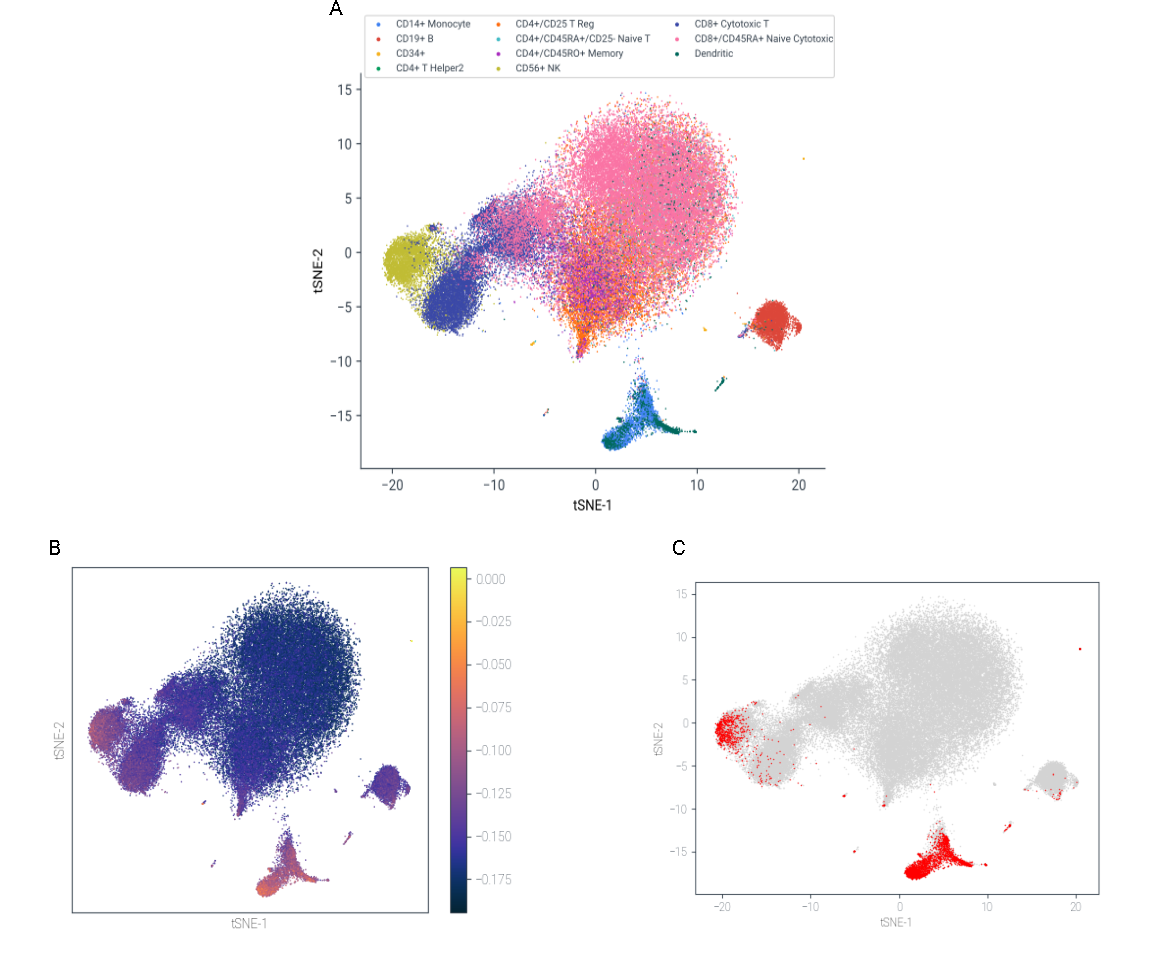
\includegraphics[width=0.9\textwidth]{DoRCSummarySI.pdf}
    \caption{
    % Performance evaluation of DoRC on PBMCs\_68k. 
    % (A) t-SNE based 2D embedding of the data with color-marked cluster identities as reported by Zheng et al. \cite{zheng2017massively}. 
    % (B) Heat map of DoRC scores for the cells on PBMCs\_68k. 
    % The cluster of megakaryocytes (0.3\%), the rarest of all the cell types are assigned the
    % highest DoRC scores.
    % (C) Rare cells identified by DoRC using IQR-thresholding-criteria
    DoRC 在 PBMCs\_68k 上的性能评估。
    (A) 基于 t-SNE 的二维嵌入数据集可视化图,按 Zheng 等所报道的鉴定的不同类别用不同的颜色标记。
    (B) PBMCs\_68k 上细胞的 DoRC 得分热图。巨核细胞群 (0.3\%),是所有细胞类型中最稀有的细胞,获得了最高的 DoRC 分数。
    (C) 使用 IQR 阈值标准后 DoRC 识别的稀有细胞。
    }
    \label{supp-fig:dorcsummary}
\end{figure*}

\begin{figure*}[!htbp]
    \centering
    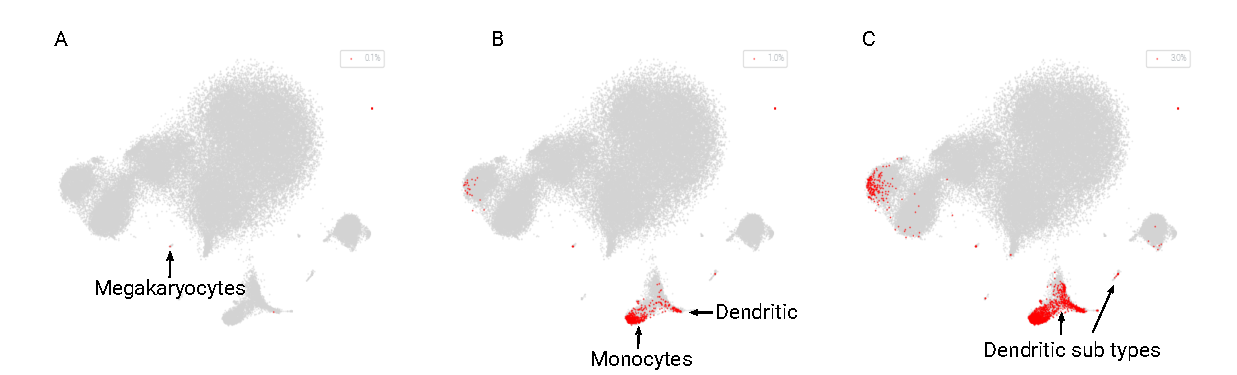
\includegraphics[width=0.9\textwidth]{DoRCSummary.pdf}
    \caption{
    % DoRC discovers cells with varying degrees of rarity. In the ${\sim}68$k PBMC data \cite{zheng2017massively}, minor cell populations with different grades of rarity show up with an
    % increase in the number of selected rare cells. (A-C) The top 0.1, 1.0 and 3.0\% cells, respectively, selected on the basis of DoRC scores are highlighted
    DoRC 发现了不同稀有度的细胞。在 ${\sim}68$k PBMC 数据 \cite{zheng2017massively} 中,不同级别的稀有度对应了一个数量不断增加的稀有细胞群。
    (A-C) 根据 DoRC 得分选出的前 0.1\%、1.0\% 和 3.0\% 的细胞分别以高亮显示。    
    }
    \label{fig:dorcsummary}
\end{figure*}

虽然连续的分数是有意义的,
如果能对细胞稀有性给出二元标注 (binary annotations),则有助于简化后续分析。
为了解决这个问题,我们引入了一个基于得分分布特性的阈值方法。
图 \ref{supp-fig:dorcsummary} C 显示了 ${\sim}68$k PBMC 数据中检测到的细胞。
我们利用基于阈值的二分法来标注稀有细胞,
如预期的那样,
大部分检测到的稀有细胞来源于已知的次要细胞类型,包括巨核细胞、树状细胞和单核细胞,
如图 \ref{supp-fig:dorcsummary} A 上所示的分别对应于 CD34+、树枝状和 CD14+ 单核细胞。



树突状细胞 (DC) 在感知、吞噬和和抗原监视 \cite{villani2017single} 方面起着至关重要的作用。
DCs 是最罕见的免疫细胞类型之一,在 PBMCs \cite{zheng2017massively} 数据集上占比约 0.5\%。
Villani \cite{villani2017single} 的研究划分了六种不同的树突状细胞的亚型。
他们通过荧光激活细胞分选 (FACS) 来分析了树突状细胞、分型 DCs 和单核细胞的表达。
他们在研究中报告的 DC 亚型如下:
$\text{CD141}^+$ DCs (DC1), 
$\text{CD1C}^+${\_}A 常规 DCs (DC2),
$\text{CD1C}^+${\_}B 常规 DCs (DC3),
$\text{CD1C}^-\text{CD141}^-$(DC4), DC5 和浆细胞 DCs (DC6,pDCs)。

我们很好奇树突状细胞亚型是否可以在 PBMCs 数据中被准确识别。
首先,我们在 ${\sim}68$k PBMCs 数据集上应用 DoRC。
DoRC 通过使用基于 IQR 的二分法,共发现了 3844 个稀有细胞。
然后通过 RafClust 对稀有细胞进行聚类 (见 \ref{subsec:rafclust}),得到 12 个子类别。
在这 12 个可区分的聚类中 (C0-C11),
C4、C5、C9 和 C11 完全由树枝状细胞组成,根据 Zheng 等人提供 \cite{zheng2017massively}的标注,
如图 \ref{fig:dorc_dendritic} A-C 所示。
对于这 4 个 DC 类别,我们进行差异表达分析,找出细胞类型特异性基因 (见 \ref{subsec:de})。
共有 21 个基因被检测为细胞类型特异性基因,使用阈值为 log2(1.5) 的 FC (fold change)。
通过将我们的差异基因与 Villani \cite{villani2017single} 报道的基因进行叠加。
我们可以有信心地解析 6 个亚型中的 5 个 (DC1、DC2、DC4、DC6) (图 \ref{fig:dorc_dendritic} D、表 \ref{supp-tbl:dendritic})。
从 \cite{villani2017single} 可以看出, DC5 是未识别的 (unresolved) 的,因为该类型是新分离出来的罕见类型。
在 t-SNE 二维嵌入图中, DC3 与 DC2 属于同一类 \cite{maaten2008visualizing}。
在 DoRC 检测到的稀有细胞上使用 RafClust 进行聚类,不能完全划分出树突状细胞亚型正确的数量。
然而,在最初 \cite{zheng2017massively}的研究中, DC1 和 DC4 也没有被聚类算法识别到。
事实上,在原始文献 \cite{zheng2017massively} 实验结果的 t-SNE 图上,
这些细胞类型在视觉上共同聚集在自身或单核细胞内。
\begin{figure}[!htbp]
    \centering
    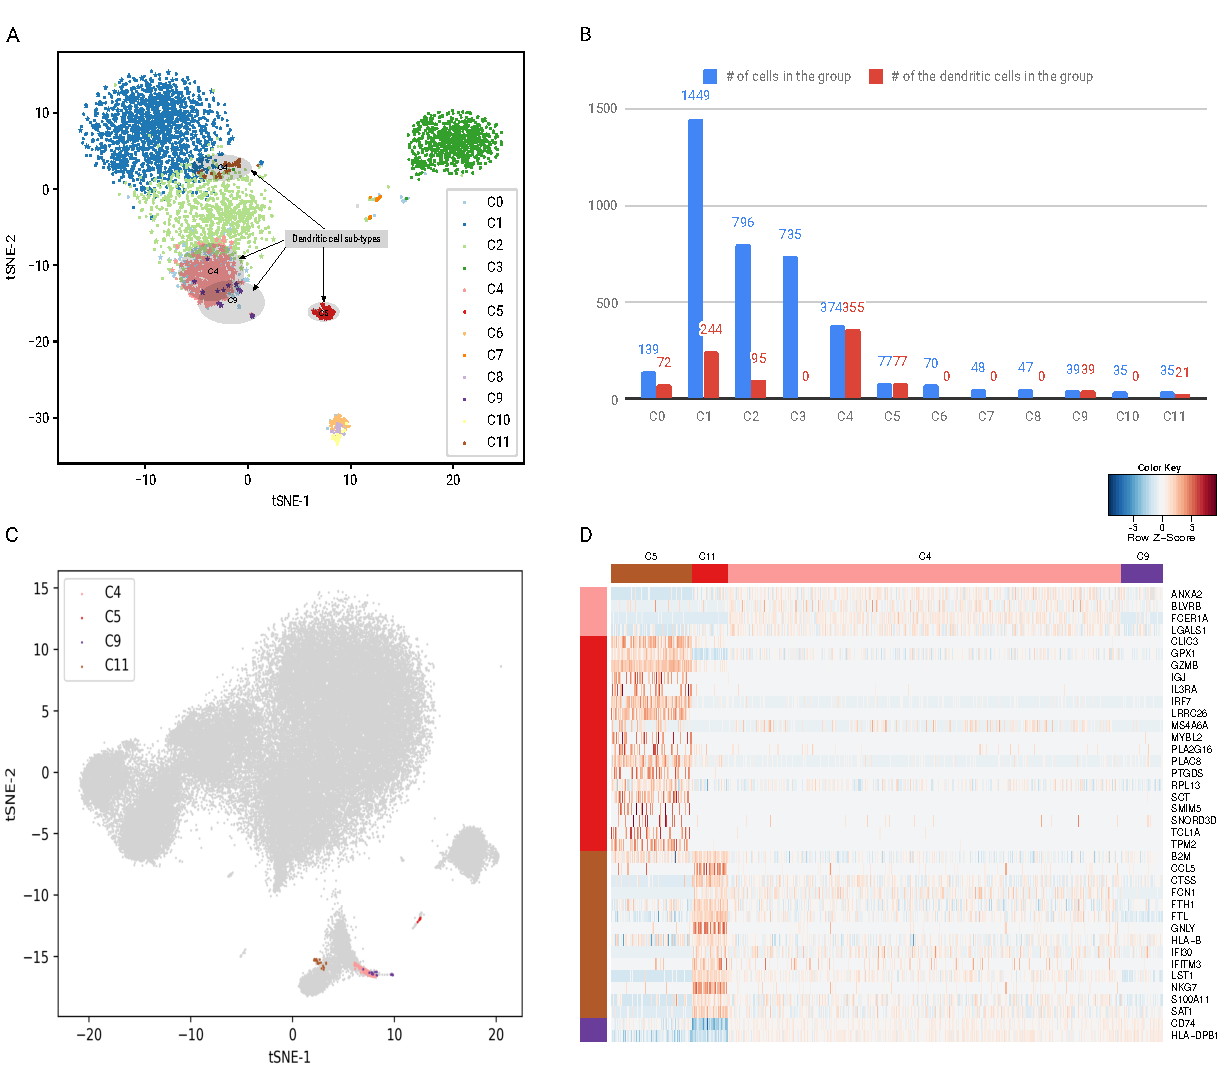
\includegraphics[width=0.9\textwidth]{plot_tsne_dorc_rare_summary.pdf}
    \caption{
    % Human blood dendritic cell heterogeneity delineated by DoRC. 
    % (A) DoRC detected rare cells are clustering into 12 sub types with RafClust, 
    % i.e. C0 (a singleton class), C1, $\ldots$, C11.
    % With the annotation given by \cite{zheng2017massively}, C4, C5, C9, C11 are mostly dendritic cells sub types.
    % Dots with the same color represent one subpopulation by clustering the rare cells with RafClust.
    % For each subpopulation, the cells annotated with asterisks marking are also dendrotic cells according to the annotation given by \cite{zheng2017massively}. 
    % (B) The cells number for each subpopulation and the number of dendrotic cells in this group. 
    % Apparently, dendritic cells hold the majority of the subpopulation in C4, C5, C9, C11.
    % (C) These four dendritic sub-types cells are highlighted on the \textit{PBMCs\_68k} dataset t-SNE-based 2D plot.
    % (D) Characterization of dendritic cell sub-types utilizing markers obtained from DE analysis (See \ref{subsec:de})
    DoRC 检测到人类血液树突状稀有细胞的异质性。
    % (A) DoRC 检测到的稀有细胞在 RafClust 中被聚成 12 个亚型,即 C0,C1,$\ldots$,C11。
    % 通过 \cite{zheng2017massively} 给出的标注, C4、C5、C9、C11 多为树枝状细胞亚型。
    % 用 RafClust 聚类稀有细胞,同种颜色的点代表一个亚群。
    % 对于每个亚群,根据 \cite{zheng2017massively} 给出的注释,
    % 用星号标记的细胞也是树突状细胞。
    % (B) 每个亚群的细胞数和本组中树突状细胞的数量。
    % 显然,树枝状细胞在 C4、C5、C9、C11 的亚群中占有多数。
    % (C) 这四种树枝状亚型细胞在 \textit{PBMCs\_68k} 数据集的 t-SNE 二维图上突出显示。
    % (D) 利用从 DE 分析中获得的标记来描述树突状细胞亚型的特征 (见节 \ref{subsec:de})
    }
    \label{fig:dorc_dendritic}
\end{figure}

\begin{table}[!htbp]
    \centering
    \caption{
        %The dendritic cell types correspond to class types reported by Villani \cite{villani2017single}
        树枝状细胞类型对应于 Villani 报告的细胞类别 \cite{villani2017single}
        }
    \label{supp-tbl:dendritic}
    \resizebox{\columnwidth}{!}{
    \begin{tabular}{clc}
    \hline
    Class type & \multicolumn{1}{c}{Marker gene(s)}                                                                                                                                   & Corresponding class type \\ \hline
    C4         & ANXA2, BLVRB, \textbf{FCER1A}, LGALS1	                                                                                                                                         & DC2                      \\ \hline
    C5         & \begin{tabular}[c]{@{}l@{}}CLIC3, GPX1, \textbf{GZMB}, \textbf{IGJ}, \textbf{IL3RA}, \textbf{IRF7}, LRRC26, MS4A6A, MYBL2,\\ PLA2G16, PLAC8, PTGDS, RPL13, SCT, SMIM5, SNORD3D, TCL1A, TPM2\end{tabular} & DC6                      \\ \hline
    C9         & \begin{tabular}[c]{@{}l@{}}B2M, CCL5, CTSS, FCN1, FTH1, \textbf{FTL}, GNLY, HLA-B, IFI30, \textbf{IFITM3}, \textbf{LST1},\\ NKG7, S100A11, SAT1\end{tabular}                                    & DC4                      \\ \hline
    C11        & CD74, \textbf{HLA-DPB1}                                                                                                                                                       & DC1                      \\ \hline
    \end{tabular}
    }

    \begin{tablenotes}
        \small
        %\item Note: Those genes marked in bold are acting as  marker genes in the corresponding class type.
        \item 注: 用粗体标记的基因在相应的类型中起着标志 (Marker) 基因的作用。
      \end{tablenotes}

\end{table}

\subsubsection{人工伪造的稀有细胞识别}
\label{subsec:recplanted} 


我们设计了一个在模拟数据集 Jurkat\_293T 上的实验来评估 DoRC 在细胞类型识别上的性能表现。
 \textit{Jurkat\_293T} 是由 Jurkat 和 293T 的两个表达谱构建的,同样来自同一研究 \cite{zheng2017massively}。
Jurkat 数据集由 3258 个细胞组成,而 293T 数据集由 2885 个细胞组成。
首先,从 293T 数据集中不放回抽样 1500 个细胞。
然后,通过从 Jurkat 数据集中取样不同数量的细胞,
产生 8 个数据集,其中 Jurkat 细胞数占比分别为 0.5\%、1\%、1.5\%、2\%、2.5\%、5\%、10\%、15\%。
这两个数据集的表达矩阵也可以从 \url{www.10xgenomics.com} 下载。
作者利用每个细胞的单核苷酸变异 (SNV) 谱来确定其系谱。
我们认为这种基于基因型的标注接近真实的细胞标签。

对于每个数据集, F1-score 是用通过 DoRC 评分和 IQR 阈值标准确定预测标签,然后与两个类的真实标签进行计算。
重复这个过程 100 次,可以得到该数据集的 F1 分数的标准差。
标准差反应了该方法识别人工伪造的稀有细胞的稳定性 (图 \ref{fig:jurkat} A)。 
F1-score 反应了精度和灵敏度之间的平衡。
当稀有率处于低水平时,即 0.5\% 和 1\% 时, DoRC 无法匹配 FiRE。
但是,当稀有率从 1.5\% 增加到 15\% 时, DoRC 的性能优于 FiRE。
此外, FiRE 的性能在 15\% 的稀有率下急剧下降,但是 DoRC 更保守,性能损失较小。

特别地,在上述 8 个数据集中,我们选取了稀有细胞占比为 2.5\% 时的对应的数据集作为基准数据集。
%从 100 个生成的数据集中随机选取了一个有 1539 个细胞的混合数据集,作为基准数据集。
从 t-SNE 图 \ref{fig:jurkat} B 上可知,该数据集上 39 个稀有细胞和 1500 个丰富细胞非常清晰地聚成两组。
在 FiRE 和 DoRC 这两种方法中,稀有细胞的得分都清晰地高于丰富细胞类型 (图 \ref{fig:jurkat} C-D)。
每种方法都得到了二元标签 (图 \ref{fig:jurkat} E-F), DoRC 的表现优于 FiRE,
因为它有更好的能力来检测更多的稀有细胞 (图 \ref{fig:jurkat} G-H)。

\begin{figure}[!htbp]
    \centering
    \includegraphics[width=0.9\textwidth]{plot_venn_dorcfire_39summary_compressed.pdf}
    \caption{
    % Detectability of minor cell types in a simulated dataset consisting of Jurkat and 293T cells. 
    % (A) The F1-scores are calculated w.r.t. the rare (Jurkat) population for DoRC and FiRE, 
    % while bioinformatically varying the proportion of artificially planted rare cells.
    % (B) The t-SNE-based 2D embedding of the cells with color-coded identities of the benchmark dataset.
    % (C-D) DoRC and FiRE score intensities plotted on the t-SNE-based 2D map, respectively. 
    % (E-F) The rare cells detected by DoRC and FiRE, respectively, are highlighted.
    % (G) DoRC, FiRE detected rare cells and true rare cells overlap with each other, shown in this Venn diagram. 
    % (H) Detail of the confusion matrices with TP, FP, FN, TN prediction metrics for DoRC and FiRE.
    在由 Jurkat 和 293T 细胞组成的模拟数据集中,次要细胞类型的可检测性示意图。
    % (A) 按照生物信息上逐渐改变人工植入的稀有细胞的比例,计算关于稀有类别 (也就是 Jurkat) 的 DoRC 和 FiRE 的 F1 分数。
    % (B) 基准数据集上细胞的基于 t-SNE 的二维嵌入可视化图,不同颜色代表不同的细胞类别。
    % (C-D) DoRC 和 FiRE 得分分别绘制在基于 t-SNE 的二维嵌入可视化图上。
    % (E-F) DoRC 和 FiRE 分别检测到的稀有细胞,用高亮来显示。
    % (G) DoRC 和 FiRE 检测到的稀有细胞和真正的稀有细胞相互重叠,在该维恩图中显示出来。
    % (H) DoRC 和 FiRE 的混淆矩阵与 TP、FP、FN、TN 指标的计算细节。
    }
    \label{fig:jurkat}
\end{figure}

\subsubsection{细胞类型敏感性与可扩展性分析}


我们设计了一项模拟研究,来分析 DoRC 评分的鲁棒性和敏感性与差异表达基因 DE 数量之间的关系。
我们生成一个由 500 个两种细胞类型组成的人工仿真的 scRNA-seq 数据 \textit{Splatter\_500}。
通过使用 R 包 Splatter \cite{zappia2017splatter},由 500 个细胞组成。
与两种细胞类型: 25 个细胞是罕见的 (也就是 rare cells),其它 475 个细胞是丰富的 (也就是 abundant cells),因此稀有细胞占总体细胞个数的 5\% 。
在这个数据集中,每个细胞有 5000 个基因。
在 R 中我们使用下面的命令来生成这个数据集:

\texttt{splatSimulate(group.prob = c(0.95, 0.05), method = groups, 
verbose = F, batchCells = 500, de.prob = c(0.4, 0.4), out.prob = 0, 
de.facLoc = 0.4, de.facScale = 0.8, nGenes = 5000)}

我们将通过严格的标准选择的差异表达基因保留在一边。
对于每次实验的迭代,我们将预先确定的 DE 基因附加到固定数量的非 DE 基因上。
我们在 1 和 150 之间改变差异表达基因的数目,来跟踪 DoRC 在检测规模小的类别细胞的敏感性。
随着给定的 DE 基因集合,计算细胞的 DoRC 分数,并对小类别细胞进行计算接收者操作特征曲线 (ROC) 下面积 (AUC)。
对于每一种数量的 DE 基因,上述过程重复 1000 次。
汇总后计算平均 AUC,以及所有的 AUC 的标准差,如图 \ref{fig:simulate:roc} 所示。
从图中可以看出,随着 DE 基因不断减少, DoRC 难以检测到次要细胞群。
然而,当引入 20 个或更多的 DE 基因时, DoRC 的预测率急剧提升。
同时,随着偏差变小,预测变得更加稳定。
另外从 t-SNE 图上可以看到,由于 DE 基因的增加,两类细胞能够更加直观地区分出来。
这个实验反应了 DoRC 对噪声具有一定的鲁棒性。

\begin{figure}[!htbp]
    \centering
    \includegraphics[width=0.9\textwidth]{simulate_panorama.pdf}
    \caption{
    % The sensitivity of DoRC to cell-type identities. 
    % On the scRNA-seq dataset \textit{Splatter\_500}, 
    % DoRC starts with recognizing the minor cell type correctly, 
    % as soon as the number of differentially expressed genes becomes adequate to give rise to a tiny cluster representing the minor cell
    % subpopulation. 
    % The top-left corner figure serves as a legend for the subsequent AUC plots. 
    % Each t-SNE and ROC plot pair serves as a representative of the 1000 repetitions of the experiment concerning a
    % specific number of differentially expressed genes. 
    % The AUC analysis is performed using cell-type annotations, 
    % and DoRC scores are assigned to individual cells.
    DoRC 对细胞类型特征敏感。
    % 在 scRNA-seq 数据集 \textit{Splatter\_500}上,
    % DoRC 从正确识别比例小的细胞类型开始,
    % 只要差异表达基因的数量变得足以产生一个代表小细胞亚群的微小簇。
    % 左上角图作为后续AUC图的图例。
    % 每个 t-SNE 和 ROC 图对对应为为 1000 次重复实验的一个代表结果,
    % 对应于一种特定数量的差异表达基因。
    % AUC 是使用各个细胞的类型标签和 DoRC 得分来计算到的。
    }
    \label{fig:simulate:roc}
\end{figure}

此外,由于 DoRC 和 FiRE 都可以给细胞做二元标注,
我们对其性能差异感到好奇。
在这个数据集中,我们考虑了 DoRC 和 FiRE 之间的 AUC、召回率、精度和 F1-score。
由于 F1-score 取决于召回率和精度,我们也包括这两个指标作为参考。
把细胞类型标注为真实标签, AUC 是用 DoRC 评分计算的。
而 F1-score是用 DoRC 评分产生的稀有度标注与 IQR 阈值标准获得的。
在两类实验中,直接构建一个混淆矩阵 (confusion matrix),其中的数值为真阳性 (TP)、假阳性 (FP)、真阴性 (TP)、假阴性 (FN)。
混淆矩阵上的精确率 Precision、召回率 Recall 计算如第 \ref{sec:locpcacmi} 章的公式 \ref{eq:precision}、\ref{eq:recall} 所示,
综合评价指标 F1-score 的计算如下面的公式 \ref{eq:f1score} 所示。
\begin{equation}
\label{eq:f1score}
\text{F1-score} = 2 \times \frac{\text{Precision} \times \text{Recall}}{ \text{Precision} + \text{Recall}}
\end{equation}

在总共 25 个稀有细胞中, DoRC 和 FiRE 都能正确检测出 23 个相同的稀有细胞。
DoRC 可以检测到其它 2 个稀有细胞和 1 个假阳性稀有细胞,
而 FiRE 未能识别出左边 2 个稀有细胞 (图 \ref{fig:simulate:venn_auc_f1} A)。
在这个数据集中, 阳性样品 (丰富细胞) 和阴性样品 (稀有细胞) 的数量是不平衡的。
这两种方法的 AUC 和精度基本没有变化,
但 DoRC 的召回率和 F1-score 均高于 FiRE (图 \ref{fig:simulate:venn_auc_f1} B)。
\begin{figure}[!htbp]
    \centering
    \includegraphics[width=0.9\textwidth]{plot_venn_dorcfire.pdf}
    \caption{
    % Comparison of DoRC and FiRE for rare cells detection in the dataset \textit{Splatter\_500}.
    % (A) Among all the 25 rare cells,  23 rare cells are all detected by DoRC and FiRE. 
    % DoRC could detect other 2 rare cells and 1 false positive rare cells, 
    % while FiRE failed to identify the left 2 rare cells.
    % (B) The AUC and precision of DoRC and FiRE are almost the same, while the Recall and  F1-score of DoRC is higher than FiRE.
    在 \textit{Splatter\_500}数据集上, DoRC 和 FiRE 对数据集中稀有细胞检测的比较。
    % (A) 在所有 25 个稀有细胞中, 23 个稀有细胞全部被 DoRC 和 FiRE 检测出来。
    % DoRC 可以检测到另外 2 个稀有细胞和 1 个假阳性稀有细胞,而 FiRE 则未能识别出剩下的 2 个稀有细胞。
    % (B) DoRC 和 FiRE 的 AUC 和精度几乎相同,而 DoRC 的 Recall 和 F1-score 高于 FiRE。
    }
    \label{fig:simulate:venn_auc_f1}
\end{figure}

DoRC 的核心算法孤立森林 (Isolation Forest) 的时间复杂度为 $O(ntlog\psi)$ \cite{liu2008isolation}。
其中 $n$、$t$ 和 $\psi$ 分别代表样本数、树的数目和每棵树的子样本数。
值得注意的是, DoRC 中的 Isolation Forest 在这种情况下没有训练的阶段。
该方法的参数我们使用默认值, t 设置为 100, $\psi$ 设置为 256。
因此, DoRC 的时间复杂度为 $O(n)$。
这个复杂度没有包括使用 RafClust 来确认稀有细胞的具体类型,
因为 FiRE 和 LOF 这两种方法也没有包含稀有细胞的类型细化这个步骤。

我们不断变化输入单细胞数据规模的大小,
分别统计出 DoRC、FiRE、GiniClust、LOF \cite{breunig2000lof} 和 RaceID 所消耗的时间,
如图 \ref{fig:timecomplexity} 所示。
测试机器为一台运行 GNU Linux/Ubuntu 16.04 操作系统 4.15.0-47-generic 内核的工作站上,
硬件配置如下: Intel(R) Xeon(R) Silver 4116 CPU @ 2.10GHz, 48 核, 64GB 内存。
DoRC 由 Python 实现,使用 scikit-learn包 (版本 0.20.2) \cite{pedregosa2011scikit}和 pyod包 (版本0.6.7)  \cite{zhao2019pyod}。
由于其它方法不能区分稀有细胞类型,在 DoRC 中我们也因此省略 RafClust 的稀有细胞类型细化的程序。
FiRE 从 \url{https://github.com/princethewinner/FiRE} 下载 (分支:master,最新提交的 abcba5b)。
因为 FiRE 的内核算法是用 C++ 编写的,我们在实验中使用的是其 Python 扩展分支。
GiniClust从 \url{https://github.com/lanjiangboston/GiniClust} 下载 (分支:master,最新提交 a442d45)。
我们在命令行界面直接使用 R 脚本,
额外的步骤包括 t-SNE 可视化和 DE 分析不计入时间对比评测中。
RaceID从 \url{https://github.com/dgrun/RaceID} 下载 (分支:master,最新提交 0a1e21c)。
LOF (local outlier factor) 是数据挖掘领域应用广泛的算法。
我们也直接使用 Pyod 包 (0.6.7版本) \cite{zhao2019pyod} 的 Python 实现 LOF。
值得注意的是, RaceID 和 GiniClust 仅输出了稀有细胞的二分标签预测,
而 DoRC、FiRE 和 LOF 则同时提供连续得分和二分标签预测。
\begin{figure}[!htbp]
    \centering
    \includegraphics[width=0.9\textwidth]{Rplot_timecomplexity.pdf}
    \caption{
    % DoRC is fast. Execution time is recorded for DoRC, FiRE, GiniClust, LOF and RaceID, while varying the number of cells from 1k to ${\sim} 68$k
    DoRC的执行速度仅次于 FiRE。我们从 1k 到 ${\sim} 68$k 逐渐改变细胞的数目, 同时记录下 DoRC、FiRE、GiniClust、LOF 和 RaceID 的执行时间。    
    }
    \label{fig:timecomplexity}
\end{figure}
图 \ref{fig:timecomplexity} 展示了从 ${\sim}68$k scRNA-seq 数据中发现稀有细胞不同方法在不同细胞输入规模时所消耗的时间。 
GiniClust 和 RaceID 要么耗时,要么耗内存;
LOF 对输入数据规模非常敏感;
然而, DoRC 和 FiRE 都是非常快的,因为它们只需要不到 2 分钟就可以完成任务。
与 DoRC 相比, FiRE 的速度明显更快。
DoRC 的实现代码可在 GitHub 仓库 \url{https://github.com/chenxofhit/DoRC} 上获取,
本节相关的实验代码和相关数据集可以根据读者的要求提供。

\subsection{小结}

RafClust 是一种纯粹的无模型 (model free) 和数据驱动 (data driven) 的方法,
不需要其它的先验信息,如细胞或基因的群体结构、通路信息等。
我们使用多种相似性度量方法刻画细胞的特征,
使用随机森林回归模型来学习细胞与细胞之间的相似性矩阵,基于相似性矩阵后采用层次聚类来决定细胞的最终类别。
该方法既支持按照指定的细胞类别数聚类, 也可以让方法自主决定细胞的类别数,
还支持聚类结果的可视化和差异基因分析。
实验结果表明, 在十个单细胞数据集上, RafClust 在 ARI 上表现优于其它六种方法。

% 近来,单细胞转录组学大大改善了我们对细胞表型性质的理解,
% 并且,还加速了新细胞类型的发现。
% 这些新的细胞类型大多是罕见的,因为显然一种丰富的细胞类型如果在很长一段时间内不被我们观察到是很不可能的。
% 一个真正稀有的细胞类型只有通过分析成千上万的细胞才能被发现。
% 虽然过去几年的技术进步使我们能够进行超高通量的单细胞测序,
% 可扩展性的稀有细胞检测方法几乎不存在。
% DoRC 避免了使用聚类作为中间步骤,
% 因为聚类方法不仅耗时,但也不可能一次性完全绘制复杂组织中的细胞类型。

进一步地在 RafClust 方法的基础上, 我们提出了一种单细胞稀有细胞识别方法 DoRC。
该方法首先给每一个细胞表达图谱都单独给出了一个细胞稀有度分数。
然后通过 IQR 阈值, DoRC 也可以像 RaceID 和 GiniClust 一样提供二元标签预测。
DoRC 使用了 Isolation Forest 作为核心算法来实现这个功能。
Isolation Forest 是机器学习中被广泛研究、应用得很广的一种无监督的异常点 (离群值) 检测方法。
每个细胞的稀有度用其在相应的高维空间中的``异常点得分"来表示。
这种做法避免了直接使用聚类作为中间步骤,高效率地直接过滤出了稀有细胞。
DoRC 在 ${\sim}68$k 人血细胞单细胞表达谱上结合 RafClust 聚类方法,能准确识别出人血树突状细胞亚型。
此外,在其它两个模拟数据集上的实验表明, DoRC 可识别人工伪造的稀有细胞并且对细胞类型特征也很敏感。
实验还表明, DoRC 是可扩展的,而且速度很快。

单细胞测序从最初在转录组、基因组中的成功应用, 逐渐席卷到包括基因组、转录组、蛋白质组、表观组等各个组学。
单细胞 RNA-seq (scRNA-seq)、单细胞 ATAC-seq (scATAC-seq)、单细胞 Hi-C (scHi-c) 等已成为最重要的数据类型。
这些数据主要从 mRNA 表达量、染色质的三维结构、染色质可达性等不同方面反应了细胞的信息。
细胞异质性研究中可以结合这三种异构数据进行融合, RafClust 中构造细胞表达的特征矩阵是后续利用随机森林算法的基础,
这个步骤十分适合结合这三种异构数据直接构造细胞的特征矩阵。
后续,我们将关注融合单细胞多元组学的数据进行细胞的异质性研究, 以及在此基础上进一步发掘稀有细胞及其类型。

% 本章中,我们提出了一种高效准确的单细胞聚类方法 RafClust。
% 我们使用多种相似性度量方法刻画细胞的特征,
% 使用随机森林回归模型来学习细胞与细胞之间的相似性矩阵,基于相似性矩阵后采用层次聚类来决定细胞的最终类别。
% 实验结果表明, 在十个单细胞数据集上, RafClust 在 ARI 上表现优于其它六种方法。

\newpage
\section{基于矩阵分解的单细胞 GRN 构建方法}
\label{sec:scgrnhunter}

\subsection{引言}

在第 \ref{sec:locpcacmi} 章和第 \ref{sec:d3grn} 章, 本文分别介绍了无向网络构建的 Loc-PCA-CMI 方法和有向网络构建的 D3GRN 方法, 
它们都是针对 DNA 微阵列测序技术下的基因表达数据集的特点提出来的方法。
当使用的数据转向了单细胞 RNA-seq 数据集的时候, 由于单细胞数据本身独有的特点, 基因调控网络的推断过程变得复杂起来。

单细胞 RNA-seq (scRNA-seq) 技术提供了单细胞水平的转录组测量。
使不同组织中细胞类型的鉴定和表示成为可能。
相比之下,传统的批量 RNA 测序的表达值是数千或数百万细胞的平均值,因此存在局限性。
单细胞 RNA-seq 技术的出现提供了一个从细胞水平研究生物机制的前所未有的视角,
能够从基因、调控、表达等多方面解释细胞变化的原因,
使得研究人员更严格地处理一些生物问题,比如组织的细胞组成、转录组的异质性,
以及细胞在发育过程中或在疾病和癌症中类型是如何的变化 \cite{kumar2017understanding,patel2014single}。

单细胞 RNA-seq (scRNA-seq) 测序技术下的数据集与 DNA 微阵列测序基因表达数据集有很大区别, 
表现在 scRNA-seq 数据集本身具有大量的细胞异质性 \cite{wagner2016revealing},
高度稀疏性导致的很多基因表达值为零 \cite{vallejos2017normalizing},
细胞与细胞之间的测序深度变化, 细胞周期相关带来的批量效应 (batch effects) \cite{buettner2015computational}。
在这种截然不同特点的数据集上如果直接应用 DNA 微阵列测序数据下的基因调控网络构建方法,
基因调控网络构建的准确性会大大降低。
%  scRNA-seq 数据集最突出的特点是细胞具有异质性,
% 在计算建模时候我们可以从表达谱数据中针对细胞进行聚类。
% 细胞聚类是 scRNA-seq 数据分析上游流程里面最基础的问题,为下游分析流程包括单细胞基因调控网络构建奠定了基础。
% 我们针对细胞异质性问题展开了研究,
% 在第 \ref{sec:rafclust} 和第 \ref{sec:dorc} 章中分别提出了一种从 scRNA-seq (单细胞 RNA-seq ) 数据进行细胞聚类的方法 RafClust 
% 和从超大规模的 scRNA-seq 数据中识别稀有细胞的方法 DoRC。
% 显然, 对应于每种细胞类型的差异表达基因跟该细胞类型的基因调控网络的构建密切相关。
% 但是,仅仅停留在构建跟细胞身份类别特征相关的基因调控网络不太完整。
%
% 上面两个章节分别介绍了无向网络构建的 Loc-PCA-CMI 方法和有向网络构建的 D3GRN 方法, 
% 它们都是针对 DNA 微阵列测序技术下的基因表达数据集的特点提出来的方法。
% 单细胞 RNA-seq (scRNA-seq) 测序技术下的数据集与基因芯片数据特点有很大区别, 
% 表现在 scRNA-seq 数据集本身具有大量的细胞异质性 \cite{wagner2016revealing},
% 高度稀疏性导致的很多基因表达值为零 \cite{vallejos2017normalizing},
% 细胞与细胞之间的测序深度变化, 细胞周期相关带来的批量效应 (batch effects) \cite{buettner2015computational}。
% 在这种截然不同特点的数据集上如果直接应用 DNA 微阵列测序数据下的基因调控网络构建方法,
% 基因调控网络构建的准确性会大大降低。
因此,针对 scRNA-seq 数据集,我们需要充分结合数据的特性,
在此基础上提出合适的基因调控网络的构建方法。

进一步地,我们认为,识别细胞的基因表达身份程序和细胞的基因表达活动程序 (如生命周期过程、对环境因素的反应) 
对于理解细胞和组织的组成至关重要。
虽然 scRNA-seq 数据可以量化成个体细胞中的转录本,
每个细胞的表达谱可能是这两种类型的程序的混合物,使它们难以分离。
在本文中,我们提出了一种基于矩阵分解的算法 WSSMFA 来解决这个问题。
在公开的大脑类器官 scRNA-seq 数据集上的实验表明,
本文提出的 scGRNHunter 方法可以准确地构建出身份和活动性的子程序, 
并在此基础之上构建基于细胞类别身份的基因调控网络和基于细胞活动的基因调控网络。

\subsection{相关工作}
在基因调控网络中,基因的协同作用,维持细胞作为特定细胞类型的身份,对外界信号作出反应,并进行复杂的如复制和代谢等细胞活动。
协调这些功能所需的基因通常是通过转录共同调控来实现的,
即基因作为一个基因表达程序 (GEP) 一起被诱导,
来响应适量的内部或外部信号 \cite{eisen1998cluster,segal2003module}。
通过对整个转录组的无偏测量, RNA-seq 等测序技术正在为系统地发现 GEPs 并揭示其支配的生物机制铺平了道路 \cite{liberzon2015molecular}。

scRNA-seq 可以让我们观察到许多的单个细胞的基因表达变化,
极大地提高了我们解析 GEPs 的能力。
即使如此, GEPs 的构建仍然具有挑战性,
因为 scRNA-seq 数据是高噪声和高维度的,因此我们需要使用合适的计算方法来挖掘潜在的模式。
此外,技术上的人为因素,如双胞 (doublets,两个或两个以上不同的细胞被错误地折叠成一个细胞) 和高度表达值缺失 (dropout) 为我们的分析增加了难度。
最近在降维、聚类、系谱轨迹追踪和差异表达分析方面的进展 \cite{amir2013visne,kharchenko2014bayesian,satija2015spatial,trapnell2014dynamics},
有助于我们解决其中的一些问题。

在本文中,我们认为从 scRNA-seq 数据中构建基因调控网络的关键是,准确构建出基因表达程序。
事实上,单个细胞可能表达多个 GEPs,但是单细胞表达谱本身只反应了它们的组合,而不是直接表达 GEPs 本身。
一个细胞的基因表达是由许多因素形成的,
包括其细胞类型,其在时间依赖性过程中的状态,如细胞周期,以及其对不同环境刺激的反应 \cite{wagner2016revealing}。
我们可以在 scRNA-seq 数据中检测到的表达程序可以归为两个大类:
\begin{enumerate}[label=(\arabic*),itemindent=2em]
    \item 对应于特定细胞类型身份,如肝细胞或黑色素细胞的 GEPs (identity program);
    \item 独立于细胞类型表达,在任何正在进行特定活动的细胞中,如细胞分裂或免疫细胞激活中表达的 GEPs (activity program)。
\end{enumerate}
在这种表述中,身份程序在特定细胞类型的细胞中唯一表达,
而活动程序在一种或多种类型的细胞中可能动态变化,并且可能是连续的或离散的。

如果由 scRNA-seq 剖析的细胞子集表达一个给定的活动 GEP,
有可能直接从数据推断程序,而不需要控制实验。
活动程序总是表达一个或常常伴随着许多细胞类型的身份程序,比确定身份 GEPs 更具有挑战性。
因此,虽然寻找相似细胞群的平均表达量往往足以找到合理准确的身份 GEPs,
但对于活动 GEPs 来说,这种做法往往会失败。

从 scRNA-seq 数据共同构建身份和活动 GEPs, 本文主要出于以下三个动机。
首先,系统地发现 GEPs 可以揭示在原生生物组织背景下意想不到的或新颖的活动程序,
反应重要的生物过程 (如免疫激活或缺氧)。
其次,它可以描述每个活动 GEP 在组织中各个细胞类型间普遍性的特征。
最后,活动程序的鉴别可以通过避免活动程序基因被错误地包含在身份程序中, 从而来改进身份程序的构建。
众所周知,对应于细胞周期不同阶段的 GEP 是广泛存在活动程序的,
并且会混淆 scRNA-seq 数据中的身份 (细胞类型) 程序构建 \cite{scialdone2015computational,chen2017controlling}。
在这项研究中, 我们提出了一个带约束的矩阵分解模型, 称为加权半非负稀疏矩阵分解的方法,
在 scRNA-seq 数据共同构建身份和活动 GEPs,然后在此基础上结合 TRRUST 这个 TF-TG (调控子-靶标基因) 数据库构建基因调控网络。
据我们所知,目前还没有文献利用类似的思路在 scRNA-seq 数据集上构建基因调控网络。

\subsection{单细胞 GRN 构建方法 scGRNHunter}

scGRNHunter 方法的流程图如图 \ref{fig:gep-flowchart} 所示, 下文我们将详细介绍流程图里的步骤。
\begin{figure}[!htbp]
    \centering
    \includegraphics[width=0.8\textwidth]{flowchart-gep.pdf}
    \caption{
        % scGRNHunter flowchart. The input is the scRNA-seq expression data 2D-matrix, whose row stands for cells, column for genes, respectively.
        % (A) Data preprocessing with the input expression data, the output is  a normalized and the column dimension reduced matrix. 
        % Highly expressed genes with a fixed number are chosen for downstream analysis.
        % (B) Cell sampling with a user-defined ratio or a fixed number of cells  from the reduced expression data. 
        % (C) GEP detection with the algorithm WSSMFA. 
        % (D) Gene regulatory network construction with TRRUST.
        scGRNHunter 流程图。输入的是 scRNA-seq 表达数据,用二维矩阵表示,其行代表细胞,列代表基因。
        (A) 用输入的表达数据进行数据预处理,输出的是经过归一化处理且列维度缩小的矩阵。
        选择固定数量的高表达基因进行下游分析。
        (B) 用用户定义的比例或固定数量的细胞从减少的表达数据中进行细胞采样。
        (C) 用 WSSMFA 算法进行 GEP 检测。
        (D) 用 TRRUST 构建基因调控网络。
    }
    \label{fig:gep-flowchart}
\end{figure}

\subsubsection{数据预处理}
由于测序技术中的噪声以及基因表达高度稀疏, 因此一般需要对单细胞数据进行预处理来控制数据质量。
通常假定输入的 scRNA-seq 数据是二维矩阵, 行代表细胞, 列代表基因, 矩阵中元素值代表细胞中对应基因的表达量。
对于每个数据集, 我们首先剔除少于 1000 个统一分子标识符 (UMIs) 检测的细胞,
然后过滤掉平均 500 个细胞中累加低于 1 个 count 的基因。
这个过滤后的计数矩阵我们表示为 $X_{ij}$ ($i=1,\ldots,C$ 个细胞, $j=1,\ldots,G$ 个基因)。
然后我们选择由 v-score \cite{klein2015droplet} 确定的 H 个分散度 (dispersion) 最高的基因作为后续输入。
对于本章中分析的所有数据集上, H 被设置为 500。

在归一化之前选择一个高分散的基因集合是至关重要的, 
因为如果噪声导致的 lower-variance 基因的信号与生物学上有意义的基因信号处在同一个量级上, 那么会对计算不利。 
H 被设置为 500, 主要考虑的是尽量包含足够多的基因保证能检测到微弱的生物信号,同时也要避免包括太多无关的基因使得计算性能欠佳。

\subsubsection{细胞抽样}
类似于 Drop-seq 等技术使得细胞测序规模比较大, 并且我们首先考虑的对象是基因 (即表达矩阵中的列), 
为了加速计算, 可以约定如果待处理的 scRNA-seq 数据上细胞规模大于一个预定的个数, 比如 5000,
我们就可以对矩阵的行 (也就是细胞) 采用行采样。
如果细胞规模个数小于该预定的数值, 直接忽略掉采样这一步, 
直接把所有的细胞纳入到后续计算之中。
 scRNA-seq 数据集下细胞采样的方法除了常见的随机采样外,还有按照细胞类型占比等比例采样 \cite{sinha2018dropclust},
考虑稀有细胞类型的影响而采用的基于几何学的采样 \cite{hie2019geometric} 等。

\subsubsection{加权半非负稀疏矩阵分解算法 WSSMFA}

\begin{figure}[!htbp]
    \centering
    \includegraphics[width=0.9\textwidth]{gep_mf.pdf}
    \caption{
        % Illustration of the algorithm WSSMFA.
        % A.Matrix factorization with the scRNA-seq data 2D-matrix. 
        % B.The objective function, where $W$ is the mask matrix, $\alpha$ and $\lambda$ are sparsity penalty parameters, and C is
        % the number of cells.
        算法 WSSMFA 的示意图。
        A. 对 scRNA-seq 数据进行矩阵因子化。
        B. WSSMFA 优化的目标函数,其中 W 为掩码矩阵, $\alpha$ 和 $\lambda$ 为稀疏度惩罚参数, C 为细胞数。
    }
    \label{fig:gep-mf}
\end{figure}

经过上述步骤处理后的 scRNA-seq 数据可以表示为一个矩阵 $X_{C \times G}$, $C$ 为细胞的数目, $G$ 为基因的数目, 
矩阵中的每个值表示该基因在对应的细胞中的表达量。
对于矩阵 $X$, 可以表示为一个因子矩阵 (factor matrix) $F_{G \times K}$ 和一个负荷矩阵 (loading matrix) $L_{C \times K}$,
并且满足 $X=LF^T$, 如图 \ref{fig:gep-mf} A 所示。 

本文设计了一个具有以下三个特征的矩阵分解目标函数:
\begin{enumerate}[label=(\arabic*),itemindent=2em]
    \item 对残差加权和的惩罚: 为了考虑基因表达值本身的不确定性,也就是 dropout 效应带来的影响,具有 dropout 值的对应位置处的残差被赋予零权重。
          通过这种方式,基因具有更确定的表达值的对最优参数估计有更大的影响。
    \item 稀疏性: 为了减少过拟合,对分解后的矩阵进行了 $l_1$ 惩罚。
    \item 分解矩阵的半非负性: 因子矩阵捕捉组织间的影响模式,因此,使因子矩阵非负易于解释是一个自然约束。
          同时,由于输入矩阵中数值可能有正有负,因此对负荷矩阵没有这样的约束。
\end{enumerate}
基于此,最终的目标函数定义如下 (如图 \ref{fig:gep-mf} B 所示):
\begin{equation}
    \label{eq:obj}
    \min _{F, L} \frac{1}{2 C}\left\|\left(X-L F^{T}\right) \odot W\right\|_{F}^{2}+\alpha\|L\|_{1}+\lambda\|F\|_{1}
\end{equation}
其中, $F$ 是非负的, $W$ 是 binary 掩码矩阵 (mask matrix), $C$ 是细胞个数,
 $\alpha$ 和 $\lambda$ 是惩罚系数。
$W$ 跟 $X$ 的维度相同,并且有:
\begin{equation}
    W_{i j}=\left\{\begin{array}{ll}1 & \text { if } x_{i j}>0 \\ 0 & \text { otherwise }\end{array}\right.
\end{equation}

这个目标函数是双凸 (biconvex) 的, 也就是说, 只在 $F$ 中凸, 或者只在给定的 $L$ 中凸, 但在两者共同变化时不是凸的。
我们使用交替最小二乘法 (Alternating Least Squares, ALS) 与梯度下降 (gradient descent) 法来优化目标函数 (算法 \ref{alg:wssmfa}, 
在 R 版本 3.5.1 中实现 \cite{goeman2012penalized,goeman2010l1})。
在每一次迭代中我们固定 F 并更新 L, 然后固定 L 并更新 F, 当两次迭代之间 F 的差值的 Frobenius 范数 < 0.01 时, 更新结束。
在每一步更新中, 优化问题都是有约束条件的线性回归。
由于线性回归的解保证了均方误差与惩罚之和最小,所以代价函数单调下降。
\begin{algorithm}
    \caption{Weighted semi-nonnegative sparse matrix factorization algorithm (WSSMFA)}
    \label{alg:wssmfa}
    \begin{algorithmic}[1]
    \Require  $X_{G \times C}$                                   \Comment{$G$ genes, $C$ cells}
    \Ensure $L_{G \times K}$, $F_{C \times K}$                \Comment{Loading matrix and factor matrix}
        \While{not converged}
            \For{$i = 1 \to G$}                                           
                \State $l_{i} \leftarrow \min _{l_{i}}\left\|\left(x_{i}-l_{i} F^{T}\right) \odot w_{i}\right\|_{F}^{2}+\alpha\left\|l_{i}\right\|_{1}$
                \State which is equivalent to 
                \State $l_{i} \leftarrow \min _{l_{i}}\left\|x_{i} \odot w_{i}-l_{i}\left(F^{T} \operatorname{diag}\left(w_{i}\right)\right)\right\|_{F}^{2}+\alpha\left\|l_{i}\right\|_{1}$
            \EndFor
            \For{$j = 1 \to C$}
                \State $f_{j} \leftarrow \min _{f_{j}}\left\|\left(x_{j}-f_{j} L^{T}\right) \odot w_{j}\right\|_{F}^{2}+\lambda \mid f_{j}\left\|_{1},\right\| f_{j} \| \geq 0$
                \State which is equivalent to 
                \State $f_{j} \leftarrow \min _{f_{j}}\left\|\left(x_{j} \odot w_{j}-f_{j}\left(L^{T} \operatorname{diag}\left(w_{j}\right)\right)\right)\right\|_{F}^{2}+\lambda\left\|f_{j}\right\|_{1},\left\|f_{j}\right\| \geq 0$
            \EndFor
        \EndWhile  
        \State \Return $L$, $F$        
  \end{algorithmic}
\end{algorithm}

\subsubsection{构建单细胞 GRN}
TRRUST (version 2, \cite{han2018trrust}) 是一个采用数据挖掘辅助建立的人类和小鼠转录调控网络数据库,并提供了网页版本的服务。
当前版本的 TRRUST 分别包含 800 个人类 TFs (调控因子) 和 828 个小鼠 TFs 的 8,444 和 6,552 个 TF-target 调控关系。
TRRUST 数据库还提供了调控模式的信息 (激活或抑制)。
目前已知调控模式的调控关系有 8972 个 (59.8\%)。

针对因子矩阵 (factor matrix) $F_{G \times K}$, 每一个因子代表了一个 GEP, 
身份 GEPs 里面的基因没有交集, 活动 GEPs 跟各个身份 GEP 之间一般存在相交的基因, 
针对身份 GEP 和活动 GEP 我们根据基因列表可以在 TRRUST 线上服务上查询关键的调控因子,然后构建基因调控网络。
%根据 GEP 结合 TRRUST 数据库找到 TF, 然后构建得到整个的基因调控网络。

\subsection{实验结果}
\subsubsection{数据集}
本章中使用的数据集如表 \ref{tab:dataset} 所示。
需要注意的是, 聚类的结果和原始的 count 矩阵在 GEO 中无法获取到,
因而本文转向从作者那里获得了聚类的标签和非规范化的原始数据。
原始的 scRNA-seq 数据中一共包含 66889 个细胞, 每个细胞包含 25984 个基因。
这些细胞总计包含 10 个类别标签。

\begin{table}[!htbp]
    \caption{\label{tab:dataset}使用的公开数据集} 
    \resizebox{\columnwidth}{!}{%  
    \begin{tabular}{lllll}
    \hline
    Author(s)                           & Year & Dataset title                                                                                                              & Dataset URL                                                                                               & Database and Identifier                                                                          \\ \hline
    \multicolumn{1}{c}{Quadrato G, et.} & 2017 & \begin{tabular}[c]{@{}l@{}}Cell diversity and network \\ dynamics in photosensitive \\ human brain organoids.\end{tabular} & \begin{tabular}[c]{@{}l@{}}https://www.ncbi.nlm.nih.gov\\ /geo/query/acc.cgi?\\ acc=GSE86153\end{tabular} & \multicolumn{1}{c}{\begin{tabular}[c]{@{}c@{}}Gene Expression Omnibus, \\ GSE86153\end{tabular}} \\
    \hline    
    \end{tabular}
    }
\end{table}

\subsubsection{模型选择}
我们需要设置 WSSMFA 算法的超参数,包括因子个数 ($K$) 和稀疏惩罚参数 ($\alpha$,$\lambda$)。
我们在 [20,25,30,35,40] 范围内评估 $K$, 在 [4.9,24.5,49,245,490] 范围内评估 $\alpha$ 和 $\lambda$。
这些范围的选择是通过考虑单细胞中的一些已知的先验知识比如类别数来定义 $K$ 的可信值,
并通过手动检查 $\alpha$ 和 $\lambda$ 变化很大的范围,
以避免对这些超参数的范围进行高分辨率搜索,导致明显不合理的解,
如因子缺乏稀疏性或者大量为空,或者与原始数据间没有关联性。

在指定的搜索空间内,我们利用之前定义的矩阵分解稳定性标准和学习因子的独立性,即代表足够的稀疏性,
对所有 $K$、$\alpha$ 和 $\lambda$ 组合的模型进行了评估。
考虑到矩阵因子化的随机性, Brunet 等人提出了一种寻找最稳定的因子化结果的方法,
这种方法已经在各种研究中得到应用 \cite{brunet2004metagenes,wu2016stability}。
我们对每个模型进行随机初始化,运行 30 次后得到共识矩阵 $C$。
$C$ 中的值在 $0$ 和 $1$ 之间,代表一对细胞被分配到同一个因子的比例。
利用 $C$ 矩阵,我们计算了共识相关性,用于衡量 $C$ 矩阵的离散程度。
共识相关度越高,说明因子矩阵越稳定。

对于每一个观察到的学习到的非空因子 $K^\textup{'}$ 的平均数 (可能小于输入的 $K$),
我们对 $\lambda$ 和 $\alpha$ 的不同取值进行了汇总,
并计算了中位共线性相关性 (cophenetic correlation,\cite{brunet2004metagenes})。
我们从考虑中剔除了任何对应于 K 的中位共时相关性 $< 0.9$ 的 $K^\textup{'}$。
接下来,在剩下的单个设置中,我们排除任何一个共线性相关性 $< 0.9$ 的参数取值。
最后,在这些明显稳定的设置中,我们根据因子对之间的最小皮尔逊相关性选择最终的超参数,
使得独立的因子和与数据中独立信号的稀疏程度相匹配。
在这里,我们计算了每对因子的皮尔逊相关性,计算一对相关矩阵的 Frobenius 范数, 
并在 30 次相同设置的随机初始化运行中取平均值。

\subsubsection{实验结果分析}
%\subsubsection{WSSMFA 揭示了基因表达程序的存在}

在大脑类器官数据集上,我们在数据预处理之后保留了 500 个分散度最高的基因 ($H = 500$),
按照 0.05\% 的比例随机采样,抽取了 2623 个细胞,按照模型选择的步骤操作后,
最终确定参数设置为: $K = 15$, $\alpha = 50$, $\lambda = 5$, 
即 15 个因子 (f1, f2, $\ldots$, f15),也就是对应 15 个 GEP。
负荷矩阵 $L$ 揭示了各细胞的表达量与因子之间的组合线性关系,我们按照细胞类别对负荷矩阵进行统计,
针对每个 GEP 我们可以画出对应类别的负荷的箱形图 (boxplot),如图 \ref{fig:gep-gep} 所示。
另外,在这个 scRNA-seq 数据使用基于 t 分布的随机邻域嵌入 (t-SNE) 方法并结合已知的细胞的类别标注信息进行二维可视化,
t-SNE 图反应了 scRNA-seq 数据中细胞分布的宏观结构,也就是可以看出 scRNA-seq 数据是否有不同的类别,即细胞是否存在异质性。
结合该数据集提供的细胞类别标签,我们对抽样之后的数据进行可视化,如图 \ref{fig:gep-tsne} 所示。

\begin{figure}[!htbp]
    \centering
    \includegraphics[width=0.9\textwidth]{GEP_Usage_Vs_Published_Clusters_QuadratoEtAI.pdf}
    \caption{
    % GEPs detected with WSSMFA.
    % GEP1, GEP2, $\ldots$, GEP15 are the 15 GEPs derived with WSSMFA algorithm.
    % For each GEP, the loading values based on the 10 different clusters,i.e. C1, C2, $\ldots$, C10,  are visualized with boxplot.
    用 WSSMFA 检测的 GEPs。
    GEP1, GEP2,$\ldots$, GEP15 是用 WSSMFA 算法计算得到的 15 个 GEP。
    对于每个 GEP,根据 10 个不同的类别,
    即 C1, C2,$\ldots$, C10,用箱形图直观地显示出其负载值。 
    }
    \label{fig:gep-gep}
\end{figure}

\begin{figure}[!htbp]
    \centering
    \includegraphics[width=0.9\textwidth]{tsne_Clusters_QuadratoEtAI.pdf}
    \caption{
    %The sampled brain organisms data visualized with t-SNE.
    采样后的大脑器官数据使用 t-SNE 可视化
    }
    \label{fig:gep-tsne}
\end{figure}


如果一个 GEP 仅仅在一个细胞类别中表达,那么它就是一个身份 GEP;
如果在两个或者多个细胞类别中表达,那么它就属于活动 GEP。
结合图 \ref{fig:gep-gep} 和图 \ref{fig:gep-tsne} 可以看出, 
GEP6 和 GEP8 是典型的身份 GEPs (分别对应到类别 C3 和 C1), GEP1、GEP9 和 GEP14 是典型的活动 GEPs。
GEP1 牵涉到类别 C2、C4、C6 和 C10; GEP14 牵涉到类别 C3、C4 和 C5。

%\subsubsection{身份调控网络与活动调控网络的构建}

结合因子矩阵 $F$,每一列中系数不为零的基因即是该因子 (也就是 GEP ) 中所包含的基因,
针对每个 GEP,我们可以结合 TRRUST (version 2) 提供的 web service 获取这些基因的 TF 从而构建其调控网络。

由 GEP6 构建的基因调控网络如图 \ref{fig:gep-grn-gep6} 所示,
该网络总共包含 30 个节点 (\textcolor{blue}{TF} 用蓝色节点表示, \textcolor{red}{TG} 用红色节点表示,下同), 41 条调控边\footnote{默认的调控方向都是 TF 调控 TG, 因此在可视化图中不显式突出边的方向。
}。
\begin{figure}[!htbp]
    \centering
    \includegraphics[width=1\textwidth]{GEP6.pdf}
    \caption{由 GEP6 构建的基因调控网络。}
    \label{fig:gep-grn-gep6}
\end{figure}

由 GEP8 构建的基因调控网络如图 \ref{fig:gep-grn-gep8} 所示。
该网络总共包含 74 个节点, 127 条调控边。
\begin{figure}[!htbp]
    \centering
    \includegraphics[width=1\textwidth]{GEP8.pdf}
    \caption{由 GEP8 构建的基因调控网络。}
    \label{fig:gep-grn-gep8}
\end{figure}

由 GEP14 构建的基因调控网络如图 \ref{fig:gep-grn-gep14} 所示。
该网络总共包含 122 个节点, 195 条调控边。
\begin{figure}[!htbp]
    \centering
    \includegraphics[width=1\textwidth]{GEP14.pdf}
    \caption{由 GEP14 构建的基因调控网络。}
    \label{fig:gep-grn-gep14}
\end{figure}

% \begin{figure}[!htbp]
%     \begin{adjustbox}{addcode={
%       \begin{minipage}{\width}}{
%           \caption{由 GEP14 构建的基因调控网络。
%           }
%           \label{fig:gep-grn-gep14}
%       \end{minipage}},rotate=90,center}
%       \includegraphics[scale=1]{GEP14.key_regulators.tsv.cs.pdf}%
%     \end{adjustbox}
%   \end{figure}

\subsection{小结}
scGRNHunter 的核心算法依赖 WSSMFA 这个矩阵分解方法,
该方法的前提假设是细胞的表达可以被建模为 GEPs 的线性组合,
这也是该方法的一个限制。
值得注意的是, 这排除了转录抑制的建模, 也就是说其中一个或多个基因将被一个 GEP 诱导,
当第二个抑制 GEP 在同一细胞中活跃时, 其表达量会显著降低。
据我们所知, 这种关系还没有在矩阵因子化框架中表示, 但它们可能更容易纳入新的潜变量模型类别,
如变分自动编码器 (Variational Auto-encoders, VAEs) \cite{ding2018interpretable,gronbech2018scvae}。
VAEs 代表了一个高度灵活的隐式空间中的建模, 可以捕捉隐式变量之间的非线性和相互作用。
然而, 虽然隐变量的设计是为了促进输入基因表达数据的准确重建, 
但它们是否可以直接或间接地解释为不同的 GEPs 相互作用, 还有待证明。
在可预见的未来, 调控关系的建模需要综合权衡考虑模型本身的灵活性与训练和解释它们的输出的难度这两个方面。

随着 RNA 捕获效率和高通量的技术不断地进步, scRNA-seq 数据可能会变得更加丰富和精准,
这将使得检测越来越细微的 GEPs, 从而捕捉细胞类型、细胞状态和活动的生物变异性,而不需要进行实验操作成为了可能。
本文提出了一个计算方法框架 scGRNHunter,
该方法使用了基于矩阵分解的算法 WSSMFA 直接从 scRNA-seq 中构建出这样的 GEPs。 
通过在公开的大脑类器官 scRNA-seq 数据集上的实验表明,
本文提出的 scGRNHunter 方法可以准确地构建出身份和活动性的子程序, 
并在此基础上构建成基于细胞类别身份的基因调控网络和基于细胞活动的基因调控网络。
scGRNHunter 为细胞和组织行为提供了至关重要的解释角度,
为基于 scRNA-seq 数据的基因调控网络的构建提供了一个全新的思路。
后续我们将结合该计算方法, 进一步寻找生物上的实验结果支撑。

% \newpage
% \section{基于孤立森林的单细胞稀有细胞识别方法}
\label{sec:dorc}

\subsection{引言}
在上一章我们提出了一种高效准确的单细胞聚类方法。
在单细胞数据上,除了聚类之外,还有一个十分具有挑战性的问题,即是如何从超大规模的~scRNA-seq~数据中识别稀有细胞。
现有的寻找稀有细胞的算法大部分依赖单细胞聚类方法,
在处理超大规模~scRNA-seq~数据时候因而变得非常耗时或者耗费内存。
本章中,我们提出了一种高效准确的方法~DoRC~(Discovery of Rare Cells)。
DoRC~产生的稀有度分数可以帮助生物学家们着重于下游分析,只对超大规模内的部分表达细胞~scRNA-seq~数据进行分析。
在超大规模的~scRNA-seq~数据~${\sim}68$k~人血细胞的单细胞表达谱上,
~DoRC~在划分人类血液树突状细胞亚型方面有突出的效果, 执行效率高。
另外,~DoRC~可以识别仿真数据集里面的稀有细胞,并且对细胞类型特征也很敏感。

\subsection{相关工作}
单细胞~RNA-seq~(scRNA-seq)~技术提供了单细胞水平的转录组测量。
使不同组织中细胞类型的鉴定和表示成为可能。
相比之下,传统的批量~RNA~测序的表达值是数千或数百万细胞的平均值,因此存在局限性。
scRNA-seq~技术的出现给研究人员提供了一个前所未有的视角,
从细胞水平上更严格地研究生物机制和处理生物问题,比如组织的细胞组成、转录组的异质性,
以及细胞在发育过程中或在疾病和癌症中类型是如何的变化~\cite{kumar2017understanding,patel2014single}。

scRNA-seq~技术的一个非常迫切和具有挑战性的应用,是从组织中的一堆细胞中捕获稀有细胞。
稀有细胞代表了生物体内的次要细胞类型,当测序细胞的数量在数百个规模时,一个孤立的离群点~(singleton)~也很值得关注。
然而,随着吞吐能力的提高,研究重点转换到次要细胞类型的发现,再也不仅仅是单纯的单个细胞。
稀有细胞类型包括循环肿瘤细胞、癌症干细胞、循环内皮细胞、内皮祖细胞、抗原特异性T细胞、不变性自然杀伤性T细胞等。
尽管丰度较低,但稀有细胞群在决定癌症的发病机制、介导免疫反应、癌症和其它疾病的血管生成等方面起着核心作用。
抗原特异性T细胞对免疫学记忆的形成至关重要~\cite{slansky2003antigen,altman1996phenotypic,manzo2015antigen}。
内皮祖细胞,来源于骨髓,已被证明是肿瘤血管生成的可靠生物标志物~\cite{kuo2012dynamics,cima2016tumor}。
干细胞可以替代受损细胞,并用于治疗帕金森氏症、糖尿病、心脏病等疾病~\cite{jang2005stem}。
循环肿瘤细胞提供了前所未有的视角,为临床管理提供了实时的线索和根据~\cite{krebs2010circulating}。

最近基于液滴~(Drop)~的单细胞转录组测序技术的发展,使得数以万计的单细胞的并行测序成为可能。
单个细胞的测序成本显著降低的情况下,稀有细胞的鉴别也变为可行。
迄今为止,已经有许多研究发表了可公开使用的转录组,细胞数量范围在~${\sim} 20$k~和~${\sim} 70$k~之间。
大规模的转录组样本通过削弱由于扩增阶段的失败所带来的影响,可以更好地捕捉到组织中的微小细胞亚群。
事实上,稀有细胞检测已经成为目前下游分析流程中的不可缺少的一环。

到目前为止,聚焦于研究怎样去检测稀有细胞转录组的算法还很少,
其中代表性的方法有~RaceID~\cite{grun2015single},~GiniClust~\cite{jiang2016giniclust}~和~FiRE~\cite{jindal2018discovery}。
RaceID~涉及到计算成本十分高昂的参数模型,并用于检测离群的表达谱值。
它使用了~\textit{k}-means~聚类这种典型的基于距离的方法和间隙统计计算,
来作为识别大量细胞类型的中间步骤。
~GiniClust~使用了双管齐下的方法,
它首先使用~Gini~系数选择信息量大的基因,
然后它使用基于密度的空间聚类应用与噪声~(DBSCAN)~\cite{ester1996density}~来发现离群细胞。
值得注意的是,~RaceID~和~GiniClust~都使用聚类步骤来区分主要和次要细胞类型。
对于超大的~scRNA-seq~数据来说,速度非常慢,而且内存使用效率低。
相比之下,~FiRE~为研究中的每一个细胞表达谱计算出一个稀有度分数。
它使用~Sketching~技术~\cite{wang2007sizing}来估计每个细胞的密度,
对于大规模细胞的低维编码来说,~FiRE~运行速度非常快。

我们提出了一种从超大规模~scRNA-seq~数据中快速检测稀有细胞的方法,命名为~DoRC。
DoRC~方法的设计灵感来自于对细胞稀有度估计的观察。
在多维空间中某一特定异常点,可以看作是机器学习中的异常检测问题。
据我们所知,~DoRC~是第一个从超大规模~scRNA-seq~数据中发现稀有细胞的异常检测方法。
在~DoRC~中,每个细胞的稀有度用每个给定点的``异常得分"来表示。
这是通过使用孤立森林~\cite{liu2008isolation}~实现的。
我们在多个真实和模拟数据集上对~DoRC~的性能进行了评估。
~DoRC~在~${\sim}68$k~这个人血细胞的单细胞表达谱数据集上能划分出人血树枝状细胞亚型。
此外,在其它两个模拟数据集上的实验表明,~DoRC~可以识别仿真数据集中的稀有细胞,
并且对细胞类型特征也很敏感。
我们的性能测试实验还表明,~DoRC~是快速可扩展的。

\subsection{基于孤立森林的单细胞稀有细胞识别方法~DoRC}
\label{sec:method}

DoRC~方法是用于从超大型~scRNA-seq~数据中发现稀有细胞,包括几个子步骤,如图~\ref{fig:flowchart}~所示, 每个步骤的细节将在下文中详述。
\begin{figure}[!htbp]
    \centering
    \includegraphics[width=\linewidth]{flowchartv4.pdf}
    % \caption{DoRC flowchart. The flowchart illustrates the processes of our proposed DoRC method for rare cells detection from ultra-large scRNA-seq data. 
    % Each annotated vignette in this figure represents the input or output visualization for the corresponding procedure. 
    % (A) The input is the scRNA-seq expression data 2D-matrix, whose row stands for cells, column for genes, respectively.
    % (B) Data preprocessing with the input expression data, the output is  a normalized and the column dimension reduced matrix. 
    % (C-D) Rare cells discovery with Isolation Forest, which are the workhorse procedures of DoRC. 
    % (C) Rare cells scoring with Isolation Forest, the output is a list of continuous anomaly scores for all the cells.
    % The scores can be visualized in the t-SNE-based 2D plot of the dataset; 
    % (D) IQR thresholding criteria for cell rarity identification, the binary annotations are also visualized in the t-SNE-based 2D plot.
    % (E) Refining rare cell types with RafClust. Notably, this sub-procedure is optional if we do not care about the types of rare cells.
    % (F) Rare cells with types visualization, different colors represent different rare cell types in the t-SNE-based 2D plot of the rare cells.
    % (G) Different expression genes analysis with different types of rare cells, the cell type specific genes are consequently obtained. 
    % }
    \caption{DoRC~流程图。该流程图展示了我们提出的从超大规模~scRNA-seq~数据中检测稀有细胞的过程。
    本图中的每个注释图代表了相应过程的输入或输出可视化。
    (A)~输入的是~scRNA-seq~表达数据二维矩阵,其中行代表细胞,列代表基因。
    (B)~用输入的表达数据进行数据预处理,输出的是一个归一化和列的维度缩减的矩阵。
    (C-D)~用~Isolation Forest~发现稀有细胞,这是~DoRC~的核心程序。
    (C)~用~Isolation Forest~进行稀有细胞评分,输出的是所有细胞的连续的异常得分向量。
    分数可以在基于~t-SNE~的数据集二维图中可视化。
    (D)~细胞稀有度识别的~IQR~阈值标准,二元标注也可以在基于~t-SNE~的二维图中可视化。
    (E)~用~RafClust~确定稀有细胞类型。值得注意的是,如果我们不关心稀有细胞的类型,这个步骤就不需要。
    (F)~稀有细胞与类型可视化,在基于~t-SNE~的稀有细胞二维图中不同的颜色代表不同的稀有细胞类型。
    (G)~对不同类型的稀有细胞进行不同的差异基因分析,从而得到细胞类型的特异基因。
    }
    \label{fig:flowchart}
\end{figure}

\subsubsection{数据规范化和基因选择}
\label{subsec:datapreprocessing} 
每个数据集上,在至少~3~个细胞中读数超过~2~的基因被保留用于下游分析,
然后使用中位数归一化。
除~\textit{Splatter\_500}~之外的其它数据集,
我们基于基于它们的相对分散度~(dispersion,即方差/均值)~与具有相似平均表达量的基因之间的预期分散度~\cite{zheng2017massively,macosko2015highly}选出~1000个变化最大的基因。
最后,将处理后的伪计数矩阵~(pseudo-count)~加~1~后进行对数变换。

\subsubsection{使用孤立森林识别稀有细胞}
\label{subsec:if} 

孤立森林是一种无模型算法,它的计算效率很高,非常适合并行计算方法的使用~\cite{hariri2018batch}。
事实证明,它在检测异常方面也是非常有效的~\cite{susto2017anomaly}。
该算法的主要优越性在于,它并不依赖于为数据设置复杂的参数配置。
相反,它利用了异常数据``少而不同"的特点。
其它大多数异常检测算法~(anomaly detection algorithms)~都是通过了解异常数据的属性分布,并将其从其它正常数据样本中分离出来,从而找到异常数据~\cite{noto2010anomaly,chen2011ordinal,das2016incorporating}。
在孤立森林中结合树结构,从数据中抽取子样本,
并根据数据集中随机选取的特征值进行随机切割。
树枝路径越长,那么该样本为异常样本的可能性越低;
相反,路径越短的树枝越有可能是异常的。
因此,每个树枝的总长度可以被看作是对指定点的异常性衡量的``异常得分"。

孤立森林~\cite{liu2008isolation,liu2012isolation}~的算法思想同任何基于树结构的聚合~(ensemble)~方法一样,
也是在基于决策树结构之上的。
在训练时,给定一个维度为~$N$~的数据集,
该算法选择一个随机的数据子样本来构建一棵二叉树。
树的分支过程通过选择一个随机维度~$x_i$,也就是一个单一的变量或特征来进行,其中~$i \in {1,2,\ldots,N}$。
如果一个给定的数据点在维度~$x_i$~的值小于~$v$,~$v$~是该维度中在最小值和最大值之间的随机值,
那么这个点就会被送到左分支;否则,就会走到右分支。
通过这种方式,树节点当前的数据被分割成两个子数据集。
这个分支过程在数据集上递归执行,直到一个点被隔离,或者达到预定的深度限制。
这个过程再次开始,用一个新的随机子样本来建立另一棵随机化树。
在建立大量的树的集合后,也就是一片森林,训练的过程就完成了。
在评分时,可以使用新的候选数据点或用于创建树的现有数据点。
根据指定点在每棵树中达到的深度,聚合的异常得分的计算式是:
\begin{equation}
    \label{as}
    s(x,n) = 2^{-E(h(x))/c(n)}
\end{equation}
其中, $E(h(x))$~是单个数据点~$x$~在所有树中达到的深度的平均值, $h(x)$~代表~$x$~在树中的深度~(高度)。 
$c(n)$~是归一化因子,定义为二叉搜索树~(BST)~中搜索失败的平均深度。
\begin{equation}
    \label{lab:as}
    c(n) = 2H(n - 1) - (2(n - 1)/n)
\end{equation}
其中~$H(i)$~为谐波数,
可由~$ln(i)~+~0.5772156649$~(欧拉常数)~\cite{liu2012isolation}估计,$n$~为建树时所用的数据点数。
$s(x,n)$~的值接近~1~表示异常,远小于~0.5~表示正常观测值。
我们在这里使用的参数默认值与文献~\cite{liu2008isolation,liu2012isolation}一样,
即在所有实验中子样本数据为~256,树的集合数目为~100。

虽然用连续值来表示异常得分十分有意义,但有时关于细胞稀有度的二元标注可以极大地简化分析流程~(pipeline)。
因此,如果一个细胞的~DoRC~得分,即聚合异常得分,大于~$q_3 + 1.5 \times IQR$,则~DoRC~将其标记为罕见,
其中~$q_3$和~$IQR$~分别表示所有细胞中~DoRC~分数的第三分位数和四分位数范围(第~75~百分位数$-$第~25~百分位数)。

\subsubsection{差异基因分析}
\label{subsec:de}

使用上一章中介绍的单细胞聚类方法~RafClust~得到了细胞的类别标签后,
我们采用~NODES~\cite{Sengupta049734}~这一快速的非参数化、差异化表达~(DE)~分析工具进行差异基因分析。
NODES~被证明比传统的基于批量细胞测序的差异分析方法~DESeq2~\cite{love2014moderated}、edgeR~\cite{robinson2010edger},
以及针对单细胞的差异表达分析方法~scde~\cite{kharchenko2014bayesian}~和~Wilcoxon~秩和检验~(Wilcoxon rank sum test)~都有效~\cite{Sengupta049734}。
以~0.05~作为~FDR~(False Discovery Rate)~的阈值,~FC~(fold change)~变化(也就是两个组间表达量的比值)~阈值默认为~log2(5)。
在~DE~基因中,在特定类中相对于其余各类显著上调的基因被命名为细胞类型特异基因。


\subsection{实验结果}

\subsubsection{数据集}
\label{subsec:datasets} 

第一个数据集~\textit{PBMCs\_68k}由~68579~个从健康供体收集的~PBMCs~组成~\cite{zheng2017massively}。
11~个纯化的~PBMCs~亚群的单细胞表达谱被用作细胞类型标签的参考。
该数据集可在~\url{www.10xgenomics.com}~下载。

%第二个数据集textit{MSE/20k}包含了来自小鼠大脑Arc-ME区域周围的~${sim} 20$k scRNA-seq图谱~\cite{campbell2017molecular}。
%作者将神经元细胞分为34个簇。
%和非神经元细胞通过二传聚类方法分为30个聚类。
%我们只关注30个非神经元集群,其中包括8092个非神经元细胞。
%数据集~(GSE93374)~是从\url{https://hemberg-lab.github.io/scRNA.seq.datasets/mouse/brain/}下载的。

第二个数据集~\textit{Jurkat\_293T}~是由~Jurkat~和~293T~的两个表达谱构建的,同样来自同一研究~\cite{zheng2017massively}。
Jurkat~数据集由~3258~个细胞组成,而~293T~数据集由~2885~个细胞组成。
首先,从~293T~数据集中不放回抽样~1500~个细胞。
然后,通过从~Jurkat~数据集中取样不同数量的细胞,
产生~8~个数据集,其中~Jurkat~细胞数占比分别为~0.5\%、1\%、1.5\%、2\%、2.5\%、5\%、10\%、15\%。
这两个数据集的表达矩阵也可以从~\url{www.10xgenomics.com}~下载。

最后一个数据集~\textit{Splatter\_500}~是一个人工仿真~scRNA-seq~数据,
通过使用~R~包~Splatter~\cite{zappia2017splatter},由~500~个细胞组成。
与两种细胞类型:~25~个细胞是罕见的~(也就是~rare cells),其它~475~个细胞是丰富的~(也就是~abundant cells)。
在这个数据集中,每个细胞有~5000~个基因。
在~R~中我们使用下面的命令来生成这个数据集:

\texttt{splatSimulate(group.prob = c(0.95, 0.05), method = groups, 
verbose = F, batchCells = 500, de.prob = c(0.4, 0.4), out.prob = 0, 
de.facLoc = 0.4, de.facScale = 0.8, nGenes = 5000)}

\subsubsection{评价指标}

在两类实验中,直接构建一个混淆矩阵~(confusion matrix),其数字为真阳性~(TP)、假阳性~(FP)、真阴性~(TP)、假阴性~(FN)。
混淆矩阵上的精确率~Precision、召回率~Recall~和综合评价指标~F1-score~可以很容易地计算,如等式~\ref{eq:precision}、\ref{eq:recall}、\ref{eq:f1score}~所示。
% \begin{equation}
%     \label{eq:precision}
%     \text{Precision} = \frac{\text{TP}}{\text{TP} + \text{FP}}
% \end{equation}
% \begin{equation}
%     \label{eq:recall}
%     \text{Recall} = \frac{\text{TP}}{\text{TP} + \text{FN}}
% \end{equation}
\begin{equation}
\label{eq:f1score}
\text{F1-score} = 2 \times \frac{\text{Precision} \times \text{Recall}}{ \text{Precision} + \text{Recall}}
\end{equation}
在模拟实验中,对于其~DoRC~分数满足~IQR~阈值的标准的被认定为是稀有细胞。
对于实验中采用的~\textit{Jurkat\_293T}~数据集,计算出~Jurkat~细胞的~F1~分数。

\subsubsection{实验结果分析}

%\subsubsection{DoRC~概览}
\label{subsec:dorc}
RaceID~和~GiniClust~都依靠无监督聚类来检测稀有细胞。
RaceID~中的~\textit{k}-means~聚类是基于距离的,
而~GiniClust~中的~DBSCAN~聚类是基于密度的。
它们都属于基于近邻的方法进行离群点检测。
基于近邻的方法假设一个离群样本与其最近邻的接近程度与该样本与数据集中大多数其它样本的接近程度有很大的差异。
聚类性能通常取决于一些参数敏感性且工作效率低下,因为不同分布的数据点之间的近似度不同。
另一个主要问题是,样本聚类的分辨率~(resolution)~问题。
一般来说,多级聚类变得至关重要,因为次要的类经常在首次筛选就被过滤掉了~\cite{campbell2017molecular}。
其它主要细胞类型会影响数据集中的表达差异,
特别是在处理大型~scRNA-seq~数据集时,情况变得更加糟糕。

为了解决上述问题,我们提出了一种从超大规模~scRNA-seq~数据中快速准确检测稀有细胞的方法,
命名为~DoRC。
DoRC~的灵感来自于我们观察到,稀有细胞在单细胞数据集里往往是``少而不同", 这跟机器学习里的样本孤立性十分契合。
孤立森林可以充分捕捉稀有细胞的特征,
其中,每个细胞的稀有性是以树枝的聚合长度为特征的。
一个细胞的聚合长度越长,该细胞与其它细胞区分的因素就越多,它成为稀有细胞的可能性就越大。
从数量上看,孤立森林中的聚合异常分数在本质上反应了稀有特性,
这为我们调查和进一步决定细胞的稀有性提供了基础。
为了说明这一点,我们将~DoRC~应用于包含~${\sim}68$k~外周血单核细胞的~scRNA-seq~数据集~(PBMCs)~的标注进行比对,
这个数据集是知名的纯化的免疫细胞亚型数据集~\cite{zheng2017massively}。
研究者首先对细胞进行了无监督聚类,
然后根据之前已知的标记对类进行注释~(图~\ref{supp-fig:dorcsummary} A)。
我们将~DoRC~的分数叠加在这一个二维图上~(图~\ref{supp-fig:dorcsummary} B)。
最高~0.1\%~的~DoRC~分数对应的是最小的, 
清晰地标注了含有巨核细胞的~CD34+~类别~(图~\ref{fig:dorcsummary} A)。
据报道,巨核细胞只含有整个细胞集的~0.3\%~\cite{zheng2017massively}。
然后,我们将这一比例从~0.1\%~增加到~1.0\%,随后又增加到~3.0\%,
然后下一批次的细胞亚型被选入扩展的稀有细胞集合中。
这些细胞包括单核细胞和树突状细胞亚型的亚类~(图~\ref{fig:dorcsummary} B-C)。
这个案例研究展示了~DoRC~在检测不同比例的稀有细胞方面的表现。

\begin{figure*}[!htbp]
    \centering
    \includegraphics[width=0.9\textwidth]{DoRCSummarySI.pdf}
    \caption{
    % Performance evaluation of DoRC on PBMCs\_68k. 
    % (A) t-SNE based 2D embedding of the data with color-marked cluster identities as reported by Zheng et al.~\cite{zheng2017massively}. 
    % (B) Heat map of DoRC scores for the cells on PBMCs\_68k. 
    % The cluster of megakaryocytes (0.3\%), the rarest of all the cell types are assigned the
    % highest DoRC scores.
    % (C) Rare cells identified by DoRC using IQR-thresholding-criteria
    DoRC~在~PBMCs\_68k~上的性能评估。
    (A)~基于~t-SNE~的二维嵌入数据集可视化图,按~Zheng~等所报道的鉴定的不同类别用不同的颜色标记。
    (B)~PBMCs\_68k~上细胞的~DoRC~得分热图。巨核细胞群~(0.3\%),是所有细胞类型中最稀有的细胞,获得了最高的~DoRC~分数。
    (C)~使用~IQR~阈值标准后~DoRC~识别的稀有细胞。
    }
    \label{supp-fig:dorcsummary}
\end{figure*}

\begin{figure*}[!htbp]
    \centering
    \includegraphics[width=0.9\textwidth]{DoRCSummary.pdf}
    \caption{
    % DoRC discovers cells with varying degrees of rarity. In the ${\sim}68$k PBMC data~\cite{zheng2017massively}, minor cell populations with different grades of rarity show up with an
    % increase in the number of selected rare cells. (A-C) The top 0.1, 1.0 and 3.0\% cells, respectively, selected on the basis of DoRC scores are highlighted
    DoRC~发现了不同稀有度的细胞。在~${\sim}68$k~PBMC~数据~\cite{zheng2017massively}~中,不同级别的稀有度对应了一个数量不断增加的稀有细胞群。
    (A-C)~根据~DoRC~得分选出的前~0.1\%、1.0\%~和~3.0\%~的细胞分别以高亮显示。    
    }
    \label{fig:dorcsummary}
\end{figure*}

虽然连续的分数是有意义的,
如果能对细胞稀有性给出二元标注~(binary annotations),则有助于简化后续分析。
为了解决这个问题,我们引入了一个基于得分分布特性的阈值方法。
图~\ref{supp-fig:dorcsummary} C~显示了~${\sim}68$k~PBMC~数据中检测到的细胞。
我们利用基于阈值的二分法来标注稀有细胞,
如预期的那样,
大部分检测到的稀有细胞来源于已知的次要细胞类型,包括巨核细胞、树状细胞和单核细胞,
如图~\ref{supp-fig:dorcsummary} A~上所示的分别对应于~CD34+、树枝状和~CD14+~单核细胞。


%\subsubsection{DoRC~揭示了树突状细胞之间的异质性}

树突状细胞~(DC)~在感知、吞噬和和抗原监视~\cite{villani2017single}~方面起着至关重要的作用。
DCs~是最罕见的免疫细胞类型之一,在~PBMCs~\cite{zheng2017massively}~数据集上占比约~0.5\%。
Villani~\cite{villani2017single}~的研究划分了六种不同的树突状细胞的亚型。
他们通过荧光激活细胞分选~(FACS)~来分析了树突状细胞、分型~DCs~和单核细胞的表达。
他们在研究中报告的~DC~亚型如下:
$\text{CD141}^+$~DCs~(DC1), 
$\text{CD1C}^+${\_}A~常规~DCs~(DC2),
$\text{CD1C}^+${\_}B~常规~DCs~(DC3),
$\text{CD1C}^-\text{CD141}^-$(DC4),~DC5~和浆细胞~DCs~(DC6,pDCs)。

我们很好奇树突状细胞亚型是否可以在~PBMCs~数据中被准确识别。
首先,我们在~${\sim}68$k PBMCs~数据集上应用~DoRC。
DoRC~通过使用基于~IQR~的二分法,共发现了~3844~个稀有细胞。
然后通过~RafClust~对稀有细胞进行聚类~(见~\ref{subsec:rafclust}),得到~12~个子类别。
在这~12~个可区分的聚类中~(C0-C11),
C4、C5、C9~和~C11~完全由树枝状细胞组成,根据~Zheng~等人提供~\cite{zheng2017massively}的标注,
如图~\ref{fig:dorc_dendritic} A-C~所示。
对于这~4~个~DC~类别,我们进行差异表达分析,找出细胞类型特异性基因~(见~\ref{subsec:de})。
共有~21~个基因被检测为细胞类型特异性基因,使用阈值为~log2(1.5)~的~FC~(fold change)。
通过将我们的差异基因与~Villani~\cite{villani2017single}~报道的基因进行叠加。
我们可以有信心地解析~6~个亚型中的~5~个~(DC1、DC2、DC4、DC6)~(图~\ref{fig:dorc_dendritic} D、表~\ref{supp-tbl:dendritic})。
从~\cite{villani2017single}~可以看出,~DC5~是未识别的~(unresolved)~的,因为该类型是新分离出来的罕见类型。
在~t-SNE~二维嵌入图中,~DC3~与~DC2~属于同一类~\cite{maaten2008visualizing}。
在~DoRC~检测到的稀有细胞上使用~RafClust~进行聚类,不能完全划分出树突状细胞亚型正确的数量。
然而,在最初~\cite{zheng2017massively}的研究中,~DC1~和~DC4~也没有被聚类算法识别到。
事实上,在原始文献~\cite{zheng2017massively}~实验结果的~t-SNE~图上,
这些细胞类型在视觉上共同聚集在自身或单核细胞内。
\begin{figure}[!htbp]
    \centering
    \includegraphics[width=0.9\textwidth]{plot_tsne_dorc_rare_summary.pdf}
    \caption{
    % Human blood dendritic cell heterogeneity delineated by DoRC. 
    % (A) DoRC detected rare cells are clustering into 12 sub types with RafClust, 
    % i.e.~C0 (a singleton class), C1, $\ldots$, C11.
    % With the annotation given by~\cite{zheng2017massively}, C4, C5, C9, C11 are mostly dendritic cells sub types.
    % Dots with the same color represent one subpopulation by clustering the rare cells with RafClust.
    % For each subpopulation, the cells annotated with asterisks marking are also dendrotic cells according to the annotation given by~\cite{zheng2017massively}. 
    % (B) The cells number for each subpopulation and the number of dendrotic cells in this group. 
    % Apparently, dendritic cells hold the majority of the subpopulation in C4, C5, C9, C11.
    % (C) These four dendritic sub-types cells are highlighted on the~\textit{PBMCs\_68k} dataset t-SNE-based 2D plot.
    % (D) Characterization of dendritic cell sub-types utilizing markers obtained from DE analysis (See~\ref{subsec:de})
    DoRC~检测到人类血液树突状稀有细胞的异质性。
    % (A)~DoRC~检测到的稀有细胞在~RafClust~中被聚成~12~个亚型,即~C0,C1,$\ldots$,C11。
    % 通过~\cite{zheng2017massively}~给出的标注,~C4、C5、C9、C11~多为树枝状细胞亚型。
    % 用~RafClust~聚类稀有细胞,同种颜色的点代表一个亚群。
    % 对于每个亚群,根据~\cite{zheng2017massively}~给出的注释,
    % 用星号标记的细胞也是树突状细胞。
    % (B)~每个亚群的细胞数和本组中树突状细胞的数量。
    % 显然,树枝状细胞在~C4、C5、C9、C11~的亚群中占有多数。
    % (C)~这四种树枝状亚型细胞在~\textit{PBMCs\_68k}~数据集的~t-SNE~二维图上突出显示。
    % (D)~利用从~DE~分析中获得的标记来描述树突状细胞亚型的特征~(见节~\ref{subsec:de})
    }
    \label{fig:dorc_dendritic}
\end{figure}

\begin{table}[!htbp]
    \centering
    \caption{
        %The dendritic cell types correspond to class types reported by Villani~\cite{villani2017single}
        树枝状细胞类型对应于~Villani~报告的细胞类别~\cite{villani2017single}
        }
    \label{supp-tbl:dendritic}
    \resizebox{\columnwidth}{!}{
    \begin{tabular}{clc}
    \hline
    Class type & \multicolumn{1}{c}{Marker gene(s)}                                                                                                                                   & Corresponding class type \\ \hline
    C4         & ANXA2, BLVRB, \textbf{FCER1A}, LGALS1	                                                                                                                                         & DC2                      \\ \hline
    C5         & \begin{tabular}[c]{@{}l@{}}CLIC3, GPX1, \textbf{GZMB}, \textbf{IGJ}, \textbf{IL3RA}, \textbf{IRF7}, LRRC26, MS4A6A, MYBL2,\\ PLA2G16, PLAC8, PTGDS, RPL13, SCT, SMIM5, SNORD3D, TCL1A, TPM2\end{tabular} & DC6                      \\ \hline
    C9         & \begin{tabular}[c]{@{}l@{}}B2M, CCL5, CTSS, FCN1, FTH1, \textbf{FTL}, GNLY, HLA-B, IFI30, \textbf{IFITM3}, \textbf{LST1},\\ NKG7, S100A11, SAT1\end{tabular}                                    & DC4                      \\ \hline
    C11        & CD74, \textbf{HLA-DPB1}                                                                                                                                                       & DC1                      \\ \hline
    \end{tabular}
    }

    \begin{tablenotes}
        \small
        %\item Note: Those genes marked in bold are acting as  marker genes in the corresponding class type.
        \item 注:~用粗体标记的基因在相应的类型中起着标志~(Marker)~基因的作用。
      \end{tablenotes}

\end{table}

% \subsubsection{DoRC~能够识别人工伪造的稀有细胞}
\label{subsec:recplanted} 
我们设计了一个模拟实验来评估~DoRC~在细胞类型识别上的性能表现。
我们使用了一个~scRNA-seq~数据集~Jurkat\_293T,由~293T~和~Jurkat~细胞在体外以不同比例混合组成~(见节~\ref{subsec:datasets})。
作者利用每个细胞的单核苷酸变异~(SNV)~谱来确定其系谱。
我们认为这种基于基因型的标注接近真实的细胞标签。

随着~Jurkat~(稀有)~细胞在所有细胞中的占比从~0.5\%~变化到~15\%,
我们得到~8~个数据集。
对于每个数据集,~F1-score~是用通过~DoRC~评分和~IQR~阈值标准确定预测标签,然后与两个类的真实标签进行计算。
重复这个过程~100~次,可以得到该数据集的~F1~分数的标准差。
标准差反应了该方法识别人工伪造的稀有细胞的稳定性~(图~\ref{fig:jurkat} A)。 
F1-score~反应了精度和灵敏度之间的平衡。
当稀有率处于低水平时,即~0.5\%~和~1\%~时,~DoRC~无法匹配~FiRE。
但是,当稀有率从~1.5\%~增加到~15\%~时,~DoRC~的性能优于~FiRE。
此外,~FiRE~的性能在~15\%~的稀有率下急剧下降,但是~DoRC~更保守,性能损失较小。

特别地,在上述~8~个数据集中,我们选取了稀有细胞占比为~2.5\%~时的对应的数据集作为基准数据集。
%从~100~个生成的数据集中随机选取了一个有~1539~个细胞的混合数据集,作为基准数据集。
从~t-SNE~图~\ref{fig:jurkat} B~上可知,该数据集上~39~个稀有细胞和~1500~个丰富细胞非常清晰地聚成两组。
在~FiRE~和~DoRC~这两种方法中,稀有细胞的得分都清晰地高于丰富细胞类型~(图~\ref{fig:jurkat} C-D)。
每种方法都得到了二元标签~(图~\ref{fig:jurkat} E-F),~DoRC~的表现优于~FiRE,
因为它有更好的能力来检测更多的稀有细胞~(图~\ref{fig:jurkat} G-H)。

\begin{figure}[!htbp]
    \centering
    \includegraphics[width=0.9\textwidth]{plot_venn_dorcfire_39summary_compressed.pdf}
    \caption{
    % Detectability of minor cell types in a simulated dataset consisting of Jurkat and 293T cells. 
    % (A) The F1-scores are calculated w.r.t. the rare (Jurkat) population for DoRC and FiRE, 
    % while bioinformatically varying the proportion of artificially planted rare cells.
    % (B) The t-SNE-based 2D embedding of the cells with color-coded identities of the benchmark dataset.
    % (C-D) DoRC and FiRE score intensities plotted on the t-SNE-based 2D map, respectively. 
    % (E-F) The rare cells detected by DoRC and FiRE, respectively, are highlighted.
    % (G) DoRC, FiRE detected rare cells and true rare cells overlap with each other, shown in this Venn diagram. 
    % (H) Detail of the confusion matrices with TP, FP, FN, TN prediction metrics for DoRC and FiRE.
    在由~Jurkat~和~293T~细胞组成的模拟数据集中,次要细胞类型的可检测性示意图。
    % (A)~按照生物信息上逐渐改变人工植入的稀有细胞的比例,计算关于稀有类别~(也就是~Jurkat)~的~DoRC~和~FiRE~的~F1~分数。
    % (B)~基准数据集上细胞的基于~t-SNE~的二维嵌入可视化图,不同颜色代表不同的细胞类别。
    % (C-D)~DoRC~和~FiRE~得分分别绘制在基于~t-SNE~的二维嵌入可视化图上。
    % (E-F)~DoRC~和~FiRE~分别检测到的稀有细胞,用高亮来显示。
    % (G)~DoRC~和~FiRE~检测到的稀有细胞和真正的稀有细胞相互重叠,在该维恩图中显示出来。
    % (H)~DoRC~和~FiRE~的混淆矩阵与~TP、FP、FN、TN~指标的计算细节。
    }
    \label{fig:jurkat}
\end{figure}

%\subsubsection{DoRC~对细胞类型敏感}

我们设计了一项模拟研究,来分析~DoRC~评分的鲁棒性和敏感性与差异表达基因~DE~数量之间的关系。
我们首先生成一个由~500~个两种细胞类型组成的人工仿真的~scRNA-seq~数据。
数量小的细胞类型约占细胞的~5\%~(见节~\ref{subsec:datasets})~。
我们将通过严格的标准选择的差异表达基因保留在一边。
对于每次实验的迭代,我们将预先确定的~DE~基因附加到固定数量的非~DE~基因上。
我们在~1~和~150~之间改变差异表达基因的数目,来跟踪~DoRC~在检测规模小的类别细胞的敏感性。
随着给定的~DE~基因集合,计算细胞的~DoRC~分数,并对小类别细胞进行计算接收者操作特征曲线~(ROC)~下面积~(AUC)。
对于每一种数量的~DE~基因,上述过程重复~1000~次。
汇总后计算平均~AUC,以及所有的~AUC~的标准差,如图~\ref{fig:simulate:roc}~所示。
从图中可以看出,随着~DE~基因不断减少,~DoRC~难以检测到次要细胞群。
然而,当引入~20~个或更多的~DE~基因时,~DoRC~的预测率急剧提升。
同时,随着偏差变小,预测变得更加稳定。
另外从~t-SNE~图上可以看到,由于~DE~基因的增加,两类细胞能够更加直观地区分出来。
这个实验反应了~DoRC~对噪声具有一定的鲁棒性。

\begin{figure}[!htbp]
    \centering
    \includegraphics[width=0.9\textwidth]{simulate_panorama.pdf}
    \caption{
    % The sensitivity of DoRC to cell-type identities. 
    % On the scRNA-seq dataset \textit{Splatter\_500}, 
    % DoRC starts with recognizing the minor cell type correctly, 
    % as soon as the number of differentially expressed genes becomes adequate to give rise to a tiny cluster representing the minor cell
    % subpopulation. 
    % The top-left corner figure serves as a legend for the subsequent AUC plots. 
    % Each t-SNE and ROC plot pair serves as a representative of the 1000 repetitions of the experiment concerning a
    % specific number of differentially expressed genes. 
    % The AUC analysis is performed using cell-type annotations, 
    % and DoRC scores are assigned to individual cells.
    DoRC~对细胞类型特征敏感。
    % 在~scRNA-seq~数据集~\textit{Splatter\_500}上,
    % DoRC~从正确识别比例小的细胞类型开始,
    % 只要差异表达基因的数量变得足以产生一个代表小细胞亚群的微小簇。
    % 左上角图作为后续AUC图的图例。
    % 每个~t-SNE~和~ROC~图对对应为为~1000~次重复实验的一个代表结果,
    % 对应于一种特定数量的差异表达基因。
    % AUC~是使用各个细胞的类型标签和~DoRC~得分来计算到的。
    }
    \label{fig:simulate:roc}
\end{figure}

此外,由于~DoRC~和~FiRE~都可以给细胞做二元标注,
我们对其性能差异感到好奇。
在这个数据集中,我们考虑了~DoRC~和~FiRE~之间的~AUC、召回率、精度和~F1-score。
由于~F1-score~取决于召回率和精度,我们也包括这两个指标作为参考。
把细胞类型标注为真实标签,~AUC~是用~DoRC~评分计算的。
而~F1-score是用~DoRC~评分产生的稀有度标注与~IQR~阈值标准获得的。
在总共~25~个稀有细胞中,~DoRC~和~FiRE~都能正确检测出~23~个相同的稀有细胞。
DoRC~可以检测到其它~2~个稀有细胞和~1~个假阳性稀有细胞,
而~FiRE~未能识别出左边~2~个稀有细胞~(图~\ref{fig:simulate:venn_auc_f1} A)。
在这个数据集中, 阳性样品~(丰富细胞)~和阴性样品~(稀有细胞)~的数量是不平衡的。
这两种方法的~AUC~和精度基本没有变化,
但~DoRC~的召回率和~F1-score~均高于~FiRE~(图~\ref{fig:simulate:venn_auc_f1} B)。
\begin{figure}[!htbp]
    \centering
    \includegraphics[width=0.9\textwidth]{plot_venn_dorcfire.pdf}
    \caption{
    % Comparison of DoRC and FiRE for rare cells detection in the dataset~\textit{Splatter\_500}.
    % (A) Among all the 25 rare cells,  23 rare cells are all detected by DoRC and FiRE. 
    % DoRC could detect other 2 rare cells and 1 false positive rare cells, 
    % while FiRE failed to identify the left 2 rare cells.
    % (B) The AUC and precision of DoRC and FiRE are almost the same, while the Recall and  F1-score of DoRC is higher than FiRE.
    在~\textit{Splatter\_500}数据集上,~DoRC~和~FiRE~对数据集中稀有细胞检测的比较。
    % (A)~在所有~25~个稀有细胞中,~23~个稀有细胞全部被~DoRC~和~FiRE~检测出来。
    % DoRC~可以检测到另外~2~个稀有细胞和~1~个假阳性稀有细胞,而~FiRE~则未能识别出剩下的~2~个稀有细胞。
    % (B)~DoRC~和~FiRE~的~AUC~和精度几乎相同,而~DoRC~的~Recall~和~F1-score~高于~FiRE。
    }
    \label{fig:simulate:venn_auc_f1}
\end{figure}

%\subsubsection{DoRC~是可扩展和快速的}
%\label{subsec:scalable} 

DoRC~的核心算法孤立森林~(Isolation Forest)~的时间复杂度为~$O(ntlog\psi)$~\cite{liu2008isolation}。
其中~$n$、$t$~和~$\psi$~分别代表样本数、树的数目和每棵树的子样本数。
值得注意的是,~DoRC~中的~Isolation Forest~在这种情况下没有训练的阶段。
该方法的参数我们使用默认值,~t~设置为~100,~$\psi$~设置为~256。
因此,~DoRC~的时间复杂度为~$O(n)$。
这个复杂度没有包括使用~RafClust~来确认稀有细胞的类型,
因为~FiRE~和~LOF~这两种方法也没有包含稀有细胞的类型细化这个步骤。

我们不断变化输入单细胞数据规模的大小,
分别统计出~DoRC、FiRE、GiniClust、LOF~\cite{breunig2000lof}~和~RaceID~所消耗的时间,
如图~\ref{fig:timecomplexity}~所示。
测试机器为一台运行~GNU Linux/Ubuntu 16.04~操作系统~4.15.0-47-generic~内核的工作站上,
硬件配置如下:~Intel(R) Xeon(R) Silver 4116 CPU @ 2.10GHz,~48~核,~64GB~内存。
DoRC~由~Python~实现,使用~scikit-learn包~(版本~0.20.2)~\cite{pedregosa2011scikit}和~pyod包~(版本0.6.7)~~\cite{zhao2019pyod}。
由于其它方法不能区分稀有细胞类型,在~DoRC~中我们也因此省略~RafClust~的稀有细胞类型细化的程序。
FiRE~从~\url{https://github.com/princethewinner/FiRE}~下载~(分支:master,最新提交的~abcba5b)。
因为~FiRE~的内核算法是用~C++~编写的,我们在实验中使用的是其~Python~扩展分支。
GiniClust从~\url{https://github.com/lanjiangboston/GiniClust}~下载~(分支:master,最新提交~a442d45)。
我们在命令行界面直接使用~R~脚本,
额外的步骤包括~t-SNE~可视化和~DE~分析不计入时间对比评测中。
RaceID从~\url{https://github.com/dgrun/RaceID}~下载~(分支:master,最新提交~0a1e21c)。
LOF~(local outlier factor)~是数据挖掘领域应用广泛的算法。
我们也直接使用~Pyod~包~(0.6.7版本)~\cite{zhao2019pyod}~的~Python~实现~LOF。
值得注意的是,~RaceID~和~GiniClust~仅输出了稀有细胞的二分标签预测,
而~DoRC、FiRE~和~LOF~则同时提供连续得分和二分标签预测。
\begin{figure}[!htbp]
    \centering
    \includegraphics[width=0.9\textwidth]{Rplot_timecomplexity.pdf}
    \caption{
    % DoRC is fast. Execution time is recorded for DoRC, FiRE, GiniClust, LOF and RaceID, while varying the number of cells from 1k to ${\sim} 68$k
    DoRC的执行速度仅次于~FiRE。我们从~1k~到~${\sim} 68$k~逐渐改变细胞的数目, 同时记录下~DoRC、FiRE、GiniClust、LOF~和~RaceID~的执行时间。    
    }
    \label{fig:timecomplexity}
\end{figure}
图~\ref{fig:timecomplexity}~展示了从~${\sim}68$k scRNA-seq~数据中发现稀有细胞不同方法在不同细胞输入规模时所消耗的时间。 
GiniClust~和~RaceID~要么耗时,要么耗内存;
LOF~对输入数据规模非常敏感;
然而,~DoRC~和~FiRE~都是非常快的,因为它们只需要不到~2~分钟就可以完成任务。
与~DoRC~相比,~FiRE~的速度明显更快。
DoRC~的实现代码可在~GitHub~仓库~\url{https://github.com/chenxofhit/DoRC}~上获取,
本章节相关的实验代码和相关数据集可以根据用户的要求提供。

\subsection{小结}
近来,单细胞转录组学大大改善了我们对细胞表型性质的理解,
并且,还加速了新细胞类型的发现。
这些新的细胞类型大多是罕见的,因为显然一种丰富的细胞类型如果在很长一段时间内不被我们观察到是很不可能的。
一个真正稀有的细胞类型只有通过分析成千上万的细胞才能被发现。
虽然过去几年的技术进步使我们能够进行超高通量的单细胞测序,
可扩展性的稀有细胞检测方法几乎不存在。
DoRC~避免了使用聚类作为中间步骤,
因为聚类方法不仅耗时,但也不可能一次性完全绘制复杂组织中的细胞类型。

DoRC~给每一个细胞表达图谱都单独给出了一个细胞稀有度分数。
通过~IQR~阈值,~DoRC~也可以像~RaceID~和~GiniClust~一样提供二元标签预测。
DoRC~是通过使用~Isolation Forest~作为核心算法实现的。
Isolation Forest~是机器学习中被广泛研究、应用得很广的一种无监督的异常点~(离群值)~检测方法。
每个细胞的稀有度用其在相应的高维空间中的``异常点得分"来表示。
DoRC~在~${\sim}68$k~人血细胞单细胞表达谱上结合~RafClust~聚类方法,能准确识别出人血树突状细胞亚型。
此外,在其它两个模拟数据集上的实验表明,~DoRC~可识别人工伪造的稀有细胞并且对细胞类型特征也很敏感。
实验还表明,~DoRC~是可扩展的,而且速度很快。


其实,除了孤立森林外,
最近在一些领域提出了这几种方法~\cite{aggarwal2015theoretical,zhao2019pyod,liu2019generative,weng2019multi}~也值得关注。
特别是当处理超大型~scRNA-seq~数据的稀有细胞发现。
据我们所知,~DoRC~是首次将异常检测方法的思想应用于稀有细胞的发现。
因此,我们相信~DoRC~在未来检测稀有细胞领域上对于生物学家来说是一个很有潜力的工具。


\newpage
\section{总结与展望}

\subsection{研究工作总结}

作为生物分化过程和生长机制中的重要一环,
基因调控网络~(GRNs)~的研究是系统生物学的基础和热点问题。
基因调控网络是通过测量基因的表达值进行预处理,
按照设计的推断策略,并结合已知的先验知识,构建得出基因之间相互作用的网络。
技术上,近十几年来,工业界和学术界在大数据、机器学习等技术上的积累和应用也十分成熟,
这为我们解决系统生物学最核心基础的基因调控网络构建的问题提供了强大的技术支撑。
数据上,这些年随着测序技术的快速发展,
基因表达数据的获取成本大幅降低,生成速度大幅加快,数据来源越来越多,数据种类越来越丰富, 数据规模也越来越大。
而且,单细胞技术的出现和成熟,为研究者从单个细胞层次测定基因的表达量提供了可能,减少了传统技术的噪声,
为基因调控网络的构建提供了更加细粒度精确的数据。
单细胞技术还能够获得不同类型和周期细胞的表达数据,
这为研究特定细胞类型中的调控网络以及参与细胞分化过程的调控网络提供了可能。
在技术和数据的双重加持下,
研究者可以利用基因调控网络来探究基因间的调控关系,发掘隐藏的功能特征,最终应用于生物信息、医学制药等领域。
目前,一个不容忽视的问题是,基因调控网络的预测准确性还有很大的提高空间,
许多疾病的发病机理以及细胞间的相互作用还有待发掘。
随着技术的进步,基因调控网络的研究经过结合计算机、医学、生物学和数学等科学,形成交叉学科,
基因调控网络在今后的生物研究中仍将会获得持续的关注, 扮演着极其重要的角色。

本研究在总结和分析已有的基因调控网络构建的基础上,主要的工作如下:

(1) 由于原始微阵列数据中存在的外部噪声、
网络结构中的拓扑稀疏性和非线性基因之间的依赖等因素,
这些方法在网络推断中会引入冗余的依赖关系。
特别是随着网络规模的增加,这些方法的表现大幅降低。
本文提出了一种基于互信息和局部结构的基因调控网络构建方法~Loc-PCA-CMI。
该方法根据基因的共表达关系来识别局部重叠基因簇,然后基于条件互信息~(PCA-CMI)~的路径一致性算法推断每个基因簇的局部网络结构,
最终通过聚合局部网络结构,也就是基因之间的依赖性网络,来构造最终的基因调控网络。
我们在~DREAM3~敲除数据集上对~LOC-PCA-CMI~进行了评估,
将其性能与其它四种基于信息理论的网络结构推断方法进行了比较。
实验结果表明,~Loc-PCA-CMI~在~DREAM3~数据集上降低了构建中冗余的依赖关系,
特别是在基因数目为~50~和~100~的网络上在~AUPR~这个评价指标上表现优于其它四种基准方法。


(2) 当前基于数据驱动方法无法构建全局网络,
本文提出了一种数据驱动的基因调控网络构建方法~D3GRN。
该方法使用了抽样的策略~(bootstrapping),
将每个目标基因的调控关系转化为函数分解问题并利用揭示网络相互作用的算法解决各个子问题。
为了弥补数据驱动方法无法构建全局网络的缺陷,
我们最后采用了基于面积的评分方法来推断最终的网络。
实验结果表明,在~DREAM4~和~DREAM5~基准数据集上,
~D3GRN~在~AUPR~这个评价指标上与其它基准方法相比具有竞争力。

(3) 当前在单细胞~RNA-seq~数据集上细胞聚类不准确,
本文提出了一种基于随机森林相似性学习的单细胞细胞聚类方法~RafClust。
该方法使用多种相关性度量方法来刻画细胞的特征, 
然后使用随机森林回归模型进一步学习细胞与细胞之间的相似性矩阵,
基于相似性矩阵后采用层次聚类来决定细胞的最终类别。
实验结果表明,在十个单细胞数据集上,~RafClust~在~ARI~上表现优于其它六种基准方法。

(4) 现有的寻找稀有细胞的算法大部分依赖单细胞聚类方法,
在处理超大规模~scRNA-seq~数据时候非常耗时或耗费内存,
本文提出了一种基于孤立森林的单细胞稀有细胞识别方法~DoRC。
该方法利用孤立森林高效地来对每个细胞产生稀有度分数,
结合阈值方法对细胞进行稀疏性的二元标注。
实验结果表明,在超大规模的单细胞~RNA-seq~数据~${\sim}68$k~人血细胞的单细胞表达谱上,
~DoRC~在划分人类血液树突状细胞亚型方面有突出的效果,执行效率高。
另外,~DoRC~可以识别仿真数据集里面的稀有细胞,并且对细胞类型特征也很敏感。


(5) 在构建单细胞基因调控网络时,识别细胞类型特征和细胞的基因表达活动程序对于理解细胞和组织的组成至关重要。
当前从单细胞~RNA-seq~数据中无法同时推断出与细胞类型相关和与细胞活动相关的基因调控网络,
本文提出了一种基于矩阵分解的基因调控网络构建方法~scGRNHunter。
该方法利用我们提出的矩阵分解算法~WSSMFA~在单细胞~RNA-seq~数据上同时分离出细胞类型程序和细胞活动程序,
然后结合公开数据库~TRRUST~构建基于每个程序的基因调控网络。
实验结果表明,在公开的大脑类器官~scRNA-Seq~数据集上,我们提出的~scGRNHunter~方法可以有效推断出身份和活动性的子程序, 
并在此基础上构建基于细胞类型的基因调控网络和基于细胞活动的基因调控网络。


\subsection{研究展望}
% 虽然相比之前的方法我们的预测结果有很大提高,在多个数据集上也表现良好,在网络结构未知的情况下对网络进行预测。
% 而网络本身是具有特定的结构和特性的,对于参数,数据集和网络结构比较敏感。
% 例如互信息本身对于某些网络的预测准确度非常高。
% 各类方法对于数据和参数非常敏感,可能某些方法对于特定数据集预测准确率非常高,
% 但这也许是一种过拟合现象,同时也说明算法本身对于该数据非常适用,
% 找出不用数据集中的网络由哪些结构组成,数据集本身具有哪些特性,
% 每种算法中的参数对于模型有多大的影响,就需要详细的实验分析。

(1) 基于互信息的调控网络结构推断改进

互信息是基于变量之间的依赖程度,从数值上来看是概率的大小,
而从结构上来看就是变量之间的位置关系和紧密程度,~MI~只考虑两两之间的信息量,
而~CMI~则考虑三者之间的关系,运用联合概率提高了预测精确度。
因此,一方面可以继续分析变量结构关系尝试改进,去识别网络中的间接调控作用。
另一方面从基因的网络结构入手,例如某些网络的部分结构很多方法都无法预测正确,
那么是否可以分析该结构来设计适用的算法,比如针对常见的~FFT motif~结构, 
然后针对性地和现有算法结合来提高准确度。

(2) 基于回归的调控网络推断改进

回归方法除了能推断出基因调控网络的结构之外,更吸引人的是它能够推断出基因之间的相互作用的方向~(即上调和下调)。
回归模型将基因调控建模转化为机器学习特征选择的问题,
即是将靶标基因的表达看作是调控基因表达之间的相互线性作用或者非线性作用的结果。
它们应用在基因调控网络构建上优点是计算效率高,网络构建准确率高,
缺点是一些非线性的模型可解释性较低参数意义不明确,缺少对生物结构的支持。
从数据驱动的角度构建基因调控网络, 注重可解释性,但是计算效率上只适合小型网络。
针对大型的基因调控网络推断,还需要借助于深度学习等技术来构建回归模型,但是需要注重深度模型的可解释性。

(3) 基于深度学习的单细胞填充和聚类方法改进

单细胞填充和聚类是单细胞数据上游分析的核心任务, 
在很大程度上是构建与细胞类型相关的基因调控网络的必要步骤。
随着高通量测序技术的发展, 需要处理的细胞数以万计, 同时大规模的单细胞表达数据也极度稀疏,
深度学习方法先天具有计算上的高效率,已经在各种生物学应用中取得成功,
包括基因组学、转录组学、蛋白质组学、结构生物学。
在填充上, 现在的主流的~dropout imputation~方法大部分是基于矩阵分解和统计模型的,
如果将矩阵分解和深度学习计算模型相结合,同时考虑融合先验知识,
比如基因和基因之间的相互作用~(比如调控,或者是共表达),
将会给单细胞的数据填充带来革命性的变化。
在聚类上,单细胞数据存在的批次效应对聚类的影响非常巨大,消除批次效应的影响,
使得同类型不同批次的细胞表达数据尽量对齐,
有研究者提出了使用深度学习而不是传统的统计学来消除单细胞测序中的批次差异的工具。
现有的聚类方法比如~Seurat Clustering~和~SC3~在处理大规模单细胞数据集时稍显不足。
基于图的聚类算法和基于深度表示学习的聚类算法,
融合比如细胞的空间位置信息~(Spatial information)或者是多元单细胞组学数据比如
单细胞~ATAC-seq~(single cell ATAC-seq, scATAC-seq)、单细胞~Hi-C~(scHi-c), 
将会有极大的学术价值和产业应用前景。

(4) 基于深度学习的基因调控网络推断方法改进

虽然深度学习在生物信息学上取得了极大的应用成就,
将深度学习技术应用到基因调控网络还存在许多挑战,考虑到生物数据的可变性以及数据来源的不同,
在一个数据集上训练的模型可能无法很好地推广到其他数据集。
基于深度学习的方法需要大量的基因表达数据和已知的基因表达调控关系,
现在的数据集要么太小无法满足算法的要求,或者是像单细胞测序数据过于稀疏,
而且深度学习模型缺乏很好的可解释性,
导致深度学习模型在基因调控网络推断中未成为主流。
在下一阶段的研究中,可以从两个角度来着手考虑:
从数据角度看,可以考虑设计深度学习算法从图像数据中表征细胞的变化,
因为虽然单细胞基因表达数据稀疏但是图像数据缺十分稠密,可以将两种异构数据结合起来;
或者考虑使用类似于~NLP~中的词嵌入模型~(word embedding)~对大规模稀疏的单细胞基因表达数据进行编码后进行后续处理;
或者是使用生成对抗网络等模型生成具有实际数据属性的模拟数据;
再或者是考虑基因表达数据融合~TF-gene调控数据集, PPI~数据, 和~DNA~甲基化数据等多模态数据。
从计算角度看, 可以把基因调控网络推断问题转化为深度学习模型擅长处理的分类问题, 
已知的~TF~和~Gene~之间的调控关系当作正样本,
TF~与~Gene~之间的调控关系预测转换为一个多分类的问题。

\newpage

}

%%%%%%%%%%%%%%%%%%%%%%%%%%%%%%%%%%%%%%%%%%%%%%%%%%
% 临时标签,用于编译时追踪正文末尾
%%%%%%%%%%%%%%%%%%%%%%%%%%%%%%%%%%%%%%%%%%%%%%%%%%

%%%%%%%%%%%%%%%%%%%%%%%%%%%%%%%%%%%%%%%%%%%%%%%%%%
% 后续内容,标题三号黑体居中,章节无编号
% --------------------------------------------%

% https://www.zhihu.com/question/29413517/answer/44358389 %
% 说明如下:
% secnumdepth 这个计数器是 LaTeX 标准文档类用来控制章节编号深度的。在 article 中,这个计数器的值默认是 3,对应的章节命令是 \subsubsection。也就是说,默认情况下,article 将会对 \subsubsection 及其之上的所有章节标题进行编号,也就是 \part, \section, \subsection, \subsubsection。LaTeX 标准文档类中,最大的标题是 \part。它在 book 和 report 类中的层级是「-1」,在 article 类中的层级是「0」。这里,我们在调用 \appendix 的时候将计数器设置为 -2,因此所有的章节命令都不会编号了。不过,一般还是会保留 \part 的编号的。所以在实际使用中,将它设置为 0 就可以了。

% 在修改过程中请注意不要破环命令的完整性

\renewcommand\appendix{\setcounter{secnumdepth}{-2}}
\appendix

% 主文件有代码去掉页眉章节编号的“.”,但这会因为bug导致无编号章节显示一个错误编号,所以这里在无编号章节之前再次重定义sectionmark。
\renewcommand{\sectionmark}[1]{\markboth{#1}{#1}}
\renewcommand{\subsectionmark}[1]{\markright{\leftmark}}
\renewcommand{\subsubsectionmark}[1]{\markright{\leftmark}}

% section 标题从这里往后改为三号黑体居中
\titleformat{\section}{\centering \zihao{3} \bfseries \heiti}{\thesection}{1em}{}
\titlespacing*{\section} {0pt}{17pt}{34pt}

% \section{参考文献} % bibliography会自动显示参考文献四个字
\addcontentsline{toc}{section}{参考文献} % 由于参考文献不是section,这句把参考文献加入目录
% \nocite{*} % 该命令用于显示全部参考文献,即使文中没引用
% cls文件中已经引入package,这里不需要调用 \bibliographystyle 了。
% \bibliographystyle{gbt7714-2005} 
	{~}
    \vspace{-16pt}
\bibliography{thesis-references}
\newpage
\titleformat{\section}{\centering \zihao{3} \bfseries \heiti}{\thesection}{1em}{}
\titlespacing*{\section} {0pt}{18pt}{32pt}
\titleformat{\subsection}{\zihao{-4} \songti}{\thesubsection}{1em}{}
\titlespacing*{\subsection} {2em}{0pt}{0pt}
\titleformat{\subsubsection}{\zihao{-4} \songti}{\thesubsubsection}{1em}{}
\titlespacing*{\subsubsection} {2em}{0pt}{0pt}
%!TEX root = ../csuthesis_main.tex
{~}
\vspace{-9pt}
\section{攻读学位期间主要研究成果} % 无章节编号

\ifblindreview
% \noindent
% (盲审隐去作者相关具体信息)
\fi
\vspace{11pt}
\subsection*{一、学术论文}

\ifblindreview

% 学位办老师要求用如下这种几乎算是单盲的格式,我也木有办法……
\subsubsection*{已录用/检索论文}
%\noindent
第一作者:
\begin{enumerate}[label={[\arabic*]},itemindent=2em,wide]

\item A novel method of gene regulatory network structure inference from gene knock-out expression data[J]. Tsinghua Science and Technology 24, no. 4 (2019): 446-455.{\bfseries \heiti(SCI 检索,JCR 3 区)} 
\item D3GRN: a data driven dynamic network construction method to infer gene regulatory networks[J]. BMC genomics 20, no. 13 (2019): 1-8.{\bfseries \heiti(SCI 检索,JCR 1 区)} 
\item DoRC: Discovery of rare cells from ultra-large scRNA-seq data[C]. In 2019 IEEE International Conference on Bioinformatics and Biomedicine (BIBM), pp. 111-116. IEEE, 2019.{\bfseries \heiti(EI 检索)}

\end{enumerate}
%第二作者:
%\begin{enumerate}[label={[\arabic*]},itemindent=2em,wide]
%\item CSU Latex Template[J]. CSU player: 1(1):1-10. {\bfseries \heiti(SCI 检索,JCR 1 区)}
%\item CSU Latex Template[J]. CSU player: 1(1):1-10. {\bfseries \heiti(SCI 检索,JCR 2 区)}
%\end{enumerate}
%\noindent
\subsubsection*{投稿状态论文}
%\noindent
第一作者:
\begin{enumerate}[label={[\arabic*]},itemindent=2em,wide]
\item scGRNHunter: a gene regulatory network reconstruction method from single cell RNA-seq data[J]. Bioinformatics. {\bfseries \heiti(SCI JCR 1 区)}
\end{enumerate}
%第二作者:
%\begin{enumerate}[label={[\arabic*]},itemindent=2em,wide]
%\item CSU Latex Template. XXX Transactions on CSU player. {\bfseries \heiti(SCI Under Review,JCR 1 区)}
%\item CSU Latex Template. XXX Transactions on CSU player. {\bfseries \heiti(SCI Under Review,JCR 2 区)}
%\end{enumerate}


\else
% 标准版本
\begin{enumerate}[label={[\arabic*]},itemindent=2em,wide]

\item \textbf{Xiang, Chen}, Min Li, Ruiqing Zheng, Siyu Zhao, Fang-Xiang Wu, Yaohang Li, and Jianxin Wang. A novel method of gene regulatory network structure inference from gene knock-out expression data. Tsinghua Science and Technology 24, no. 4 (2019): 446-455.{\bfseries \heiti(SCI 检索,JCR 2 区)} 
\item \textbf{Xiang, Chen}, Min Li, Ruiqing Zheng, Fang-Xiang Wu, and Jianxin Wang. D3GRN: a data driven dynamic network construction method to infer gene regulatory networks. BMC genomics 20, no. 13 (2019): 1-8.{\bfseries \heiti(SCI 检索,JCR 1 区)} 
\item \textbf{Xiang, Chen}, Fang-Xiang Wu, Jin Chen, and Min Li. DoRC: Discovery of rare cells from ultra-large scRNA-seq data. In 2019 IEEE International Conference on Bioinformatics and Biomedicine (BIBM), pp. 111-116. IEEE, 2019.{\bfseries \heiti(EI 检索, CCF B~类推荐国际会议)}
\item \textbf{Xiang, Chen}, Min Li, Ruiqing Zheng, Fang-Xiang Wu, and Jianxin Wang. scGRNHunter: a gene regulatory network reconstruction method from single cell RNA-seq data. Bioinformatics. {\bfseries \heiti(拟投稿)}
\item Ruiqing Zheng, Min Li, \textbf{Xiang Chen}, Fang-Xiang Wu, Yi Pan, and Jianxin Wang. BiXGBoost: a scalable, flexible boosting-based method for reconstructing gene regulatory networks. Bioinformatics 35, no. 11 (2019): 1893-1900. {\bfseries \heiti(SCI 检索,JCR 1 区)}
\item Ruiqing Zheng, Min Li, \textbf{Xiang Chen}, Siyu Zhao, Fang-Xiang Wu, Yi Pan, Jianxin Wang. An ensemble method to reconstruct gene regulatory networks based on multivariate adaptive regression splines. IEEE/ACM Transactions on Computational Biology and Bioinformatics. DOI: 10.1109/TCBB.2019.2900614  {\bfseries \heiti(SCI 检索,JCR 1 区)}
\item Ruiqing Zheng, Zhenlan Liang, \textbf{Xiang Chen}, Yu Tian, Min Li. An Adaptive Sparse Subspace Clustering for Cell Type Identification. Front Genet. 2020 Apr 28;11:407. doi: 10.3389/fgene.2020.00407.{\bfseries \heiti(SCI 检索,JCR 2 区)}
\item Hui Jiang, Mengyun Yang, \textbf{Xiang Chen}, Min Li, Yaohang Li, and Jianxin Wang. miRTMC: A miRNA Target Prediction Method Based on Matrix Completion Algorithm[J]. IEEE JOURNAL OF BIOMEDICAL AND HEALTH INFORMATICS. 2020, DOI:10.1109/JBHI.2020.2987034. {\bfseries \heiti(SCI 检索,JCR 1 区)}
\item 王荣,王建新,\textbf{陈向},盛羽.面向异构资源集成的数字图像实验平台[J].计算机工程与应用 54, no.15 (2018):185-191.{\bfseries \heiti(EI 期刊)}
\end{enumerate}
\fi

\vspace{22pt}
\subsection*{二、主持和参与的科研项目}
\ifblindreview
\else
\begin{enumerate}[label={[\arabic*]},itemindent=2em,wide]

    \item 国家自然科学基金优秀青年项目:~生物信息学,~项目编号:61622213,参与。

\end{enumerate}

\fi

\newpage

\ifblindreview
\else
% 由于 acknowledgement 比较长,单独使用一个文件来汇总。FIXME:chenxofhit@gmail.com
\section{致谢} % 无章节编号

六年的博士生涯就要画上一个句点,行笔至此,黯然神伤不能自已。
回想自己从程序员转变为科研工作者,
从师弟转变为师兄,
从单身转变为两个孩子的父亲,
沧海变桑田,仿佛过了很久,恍惚又觉得是刹那之间。
这六年的研究生涯,也许是我人生之旅压力最大、自我反思最为频繁的时段,
幸好有幸遇到了各位良师益友,和家人的陪伴,
常思奋不顾身以全力以赴,然而个人能力实在有限,但是只取得了一点点成绩,也留下很多遗憾。
博士阶段从本质上讲是一种不断思考、不断妥协、不断前进的生活状态,
学位只在其表,
博士虽然即将结束了但这种状态将会常伴一生。

首先要万分感谢我的导师李敏教授,亦师亦友。
六年里面耳濡目染,学术上严谨、认真,有目标,有计划,敢想敢执行;
工作上认真负责,一丝不苟,不骄不躁;
生活上待人接物温文尔雅,让人如沐春风。
论文的最初的选题立意和旷日持久的实验,离不开李老师的谆谆教导。
生活上李老师给予了我极大的帮助,排忧解难,让我安心科研。
祝李老师万事如意、身体健康,永远美丽,永远幸福。
十分感谢王建新教授、潘毅教授、吴方向教授、王伟平教授、黎耀航教授。
王建新老师学术渊博,潘毅老师幽默风趣,吴方向老师严谨认真,王伟平老师知性睿智,黎耀航老师亲和有为。
他们在学术上功力深厚,看问题一针见血,散发着独特的人格魅力。
高山仰止,景行行止,虽不能至,然心向往之。
感谢丁小军老师、钟坚成老师、罗军伟老师、罗慧敏老师、彭晓清老师、刘锦老师、李洪东老师,
感谢您们对我生活和学业上的无私帮助和指导,祝您们步步高升。
感谢段桂华老师、盛羽老师,感谢您们这些年对实验室的支持。

其次我要感谢生物组这个大家庭,
感谢~213、216~实验室的各位同学,六年时间遇到了太多值得学习的师兄师姐师弟和师妹,
他们身上闪烁着对知识的渴望,对生活的热爱和对自我的不断超越,点点滴滴时刻让我深受鼓舞、不敢懈怠。
同学名单很长,但恐有遗漏,故不在这里详细罗列,转而在网络上维护一份列表\footnote{https://github.com/chenxofhit/PhdThesis/tree/master/acknowledgement.txt}。
在他们身上我学到了许多,祝你们学业和事业心想事成,幸福美满。

再次要感谢我的父母、岳父岳母、妻子、哥哥嫂子,还有两个可爱的女儿。
身体发肤受之于父母,父母的爱如高山流水长;
岳父岳母是再生父母,他们的恩情深沉而博大。
四位老人年逾天命,两鬓霜凝,六年时间里,间断帮我抚养小孩,接济不时之需,
观父母容颜渐改,垂垂老矣,我狠未能建功立业,每每念及至此羞愧难当。
结草衔环,当终身不忘。
感谢妻子的默默陪伴,与我组建了一个美满的家庭,
让你受了很多苦,有时候惹你生气,大部分时候是我错了。
希望一如既往,携手前进,白头偕老。
哥哥和嫂子远在深圳,这六年间替我扛下了父母赡养之事代行子女之孝,
在生活上和思想上给了我诸多帮助和启发,谢谢你们的支持和付出!
还要谢谢我的两个女儿陈康羲和陈康和,你们的降临给家庭带来了无穷的欢乐和喜悦,
也祝你们永远幸福快乐健康。

最后感谢中南大学给了我这样的学习机会, 
让我在一流的平台里遇到诸多良师益友,
安心学习和享受生活。
祝愿中南大学计算机学院在王建新院长的带领下, 
在诸位老师的辛勤耕耘下,桃李满天下,更上一层楼。
在我的本科和硕士论文的致谢末尾都有一句海子的诗,在此也献给读到这里的每一个人:
愿你有一个灿烂的前程,愿你有情人终成眷属,愿你在尘世获得幸福。
\newpage
\fi

\end{document}
